
    \documentclass{article}
    \usepackage[a4paper, left=1cm, right=1cm, top=2cm, bottom=2cm]{geometry}
    \usepackage{hyperref} % für anklickbare Bezüge 
    \usepackage{tikz} % für MO-Schemata
    \usepackage{amsmath}
    
    \setlength{\parindent}{0pt}
    \hypersetup{colorlinks=true, linkcolor=black, citecolor=black}% damit Referenzen nicht in PDF umklammert
    \begin{document}
    
    \pagestyle{empty}
    \tableofcontents 
    \newpage 
    
    \section{Orbitale und deren Symmetrie}
%    In der Sortierung: oben rechts $a_u$, oben links $b_{1u}$, unten links $b_{2g}$ und unten rechts $b_{3g}$ folgt: \\
%\includegraphics[scale=0.125]{img/DimerZOrbitalordnung-gesamt-MO-C6H6-beiWW.pdf}
\vspace{2cm}
\newpage \section{Linearkombinationen: 2 Monomer- / 1 Dimer-Zustände}

\[+\left(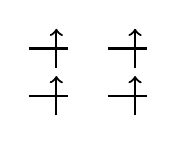
\begin{tikzpicture}
    % oberste MOs:
    \draw[thick] (0,0) -- (0.5,0); % erster Strich
    \draw[thick] (1,0) -- (1.5,0); % zweiter Strich
    % unterste MOs:
    \draw[thick] (0,-0.6) -- (0.5,-0.6); % dritter Strich
    \draw[thick] (1,-0.6) -- (1.5,-0.6); % vierter Strich
\draw[->, thick] (0.35, -0.25) -- (0.35, 0.25); 
\draw[->, thick] (1.35, -0.25) -- (1.35, 0.25); 
\draw[-> , thick] (0.35, -0.85) -- (0.35, -0.35); 
 \draw[-> , thick] (1.35, -0.85) -- (1.35, -0.35); 
\end{tikzpicture} \qquad 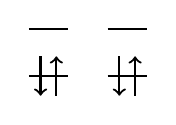
\begin{tikzpicture}
    % oberste MOs:
    \draw[thick] (0,0) -- (0.5,0); % erster Strich
    \draw[thick] (1,0) -- (1.5,0); % zweiter Strich
    % unterste MOs:
    \draw[thick] (0,-0.6) -- (0.5,-0.6); % dritter Strich
    \draw[thick] (1,-0.6) -- (1.5,-0.6); % vierter Strich
\draw[-> , thick] (0.35, -0.85) -- (0.35, -0.35); 
\draw[<- , thick] (0.15, -0.85) -- (0.15, -0.35); 
 \draw[-> , thick] (1.35, -0.85) -- (1.35, -0.35); 
\draw[<- , thick] (1.15, -0.85) -- (1.15, -0.35); 
\end{tikzpicture}\right)\]$$+\cdot \underbrace{(b_{1u}^{l})\cdot (a_{u}^{l})\cdot (b_{2g}^{l})\cdot (b_{3g}^{l})}_{\text{l: }a_{g}}\Rightarrow +\left|(b_{1u}^{l}) \cdot (b_{2g}^{l}) \cdot (b_{3g}^{l}) \cdot (a_{u}^{l})\right|$$$$=+\left|(+a_{g}+b_{1u}) \cdot (+b_{3u}+b_{2g}) \cdot (+b_{2u}+b_{3g}) \cdot (+b_{1g}+a_{u})\right|$$\begin{multline*}
=+\left|\underbrace{\overbrace{a_{g} b_{3u} b_{2u} b_{1g}}^{1 2 3 4}}_{a_{g}}\right|+\left|\underbrace{\overbrace{a_{g} b_{3u} b_{2u} a_{u}}^{1 2 3 8}}_{b_{1u}}\right|+\left|\underbrace{\overbrace{a_{g} b_{3u} b_{3g} b_{1g}}^{1 2 7 4}}_{b_{1u}}\right|+\left|\underbrace{\overbrace{a_{g} b_{3u} b_{3g} a_{u}}^{1 2 7 8}}_{a_{g}}\right|\\
+\left|\underbrace{\overbrace{a_{g} b_{2g} b_{2u} b_{1g}}^{1 6 3 4}}_{b_{1u}}\right|+\left|\underbrace{\overbrace{a_{g} b_{2g} b_{2u} a_{u}}^{1 6 3 8}}_{a_{g}}\right|+\left|\underbrace{\overbrace{a_{g} b_{2g} b_{3g} b_{1g}}^{1 6 7 4}}_{a_{g}}\right|+\left|\underbrace{\overbrace{a_{g} b_{2g} b_{3g} a_{u}}^{1 6 7 8}}_{b_{1u}}\right|\\
+\left|\underbrace{\overbrace{b_{1u} b_{3u} b_{2u} b_{1g}}^{5 2 3 4}}_{b_{1u}}\right|+\left|\underbrace{\overbrace{b_{1u} b_{3u} b_{2u} a_{u}}^{5 2 3 8}}_{a_{g}}\right|+\left|\underbrace{\overbrace{b_{1u} b_{3u} b_{3g} b_{1g}}^{5 2 7 4}}_{a_{g}}\right|+\left|\underbrace{\overbrace{b_{1u} b_{3u} b_{3g} a_{u}}^{5 2 7 8}}_{b_{1u}}\right|\\
+\left|\underbrace{\overbrace{b_{1u} b_{2g} b_{2u} b_{1g}}^{5 6 3 4}}_{a_{g}}\right|+\left|\underbrace{\overbrace{b_{1u} b_{2g} b_{2u} a_{u}}^{5 6 3 8}}_{b_{1u}}\right|+\left|\underbrace{\overbrace{b_{1u} b_{2g} b_{3g} b_{1g}}^{5 6 7 4}}_{b_{1u}}\right|+\left|\underbrace{\overbrace{b_{1u} b_{2g} b_{3g} a_{u}}^{5 6 7 8}}_{a_{g}}\right|
\end{multline*}\begin{multline*}
=+\left|\underbrace{\overbrace{a_{g} b_{3u} b_{2u} b_{1g}}^{1 2 3 4}}_{a_{g}}\right|+\left|\underbrace{\overbrace{a_{g} b_{3u} b_{2u} a_{u}}^{1 2 3 8}}_{b_{1u}}\right|-\left|\underbrace{\overbrace{a_{g} b_{3u} b_{1g} b_{3g}}^{1 2 4 7}}_{b_{1u}}\right|+\left|\underbrace{\overbrace{a_{g} b_{3u} b_{3g} a_{u}}^{1 2 7 8}}_{a_{g}}\right|\\
+\left|\underbrace{\overbrace{a_{g} b_{2u} b_{1g} b_{2g}}^{1 3 4 6}}_{b_{1u}}\right|-\left|\underbrace{\overbrace{a_{g} b_{2u} b_{2g} a_{u}}^{1 3 6 8}}_{a_{g}}\right|+\left|\underbrace{\overbrace{a_{g} b_{1g} b_{2g} b_{3g}}^{1 4 6 7}}_{a_{g}}\right|+\left|\underbrace{\overbrace{a_{g} b_{2g} b_{3g} a_{u}}^{1 6 7 8}}_{b_{1u}}\right|\\
-\left|\underbrace{\overbrace{b_{3u} b_{2u} b_{1g} b_{1u}}^{2 3 4 5}}_{b_{1u}}\right|+\left|\underbrace{\overbrace{b_{3u} b_{2u} b_{1u} a_{u}}^{2 3 5 8}}_{a_{g}}\right|-\left|\underbrace{\overbrace{b_{3u} b_{1g} b_{1u} b_{3g}}^{2 4 5 7}}_{a_{g}}\right|-\left|\underbrace{\overbrace{b_{3u} b_{1u} b_{3g} a_{u}}^{2 5 7 8}}_{b_{1u}}\right|\\
+\left|\underbrace{\overbrace{b_{2u} b_{1g} b_{1u} b_{2g}}^{3 4 5 6}}_{a_{g}}\right|+\left|\underbrace{\overbrace{b_{2u} b_{1u} b_{2g} a_{u}}^{3 5 6 8}}_{b_{1u}}\right|-\left|\underbrace{\overbrace{b_{1g} b_{1u} b_{2g} b_{3g}}^{4 5 6 7}}_{b_{1u}}\right|+\left|\underbrace{\overbrace{b_{1u} b_{2g} b_{3g} a_{u}}^{5 6 7 8}}_{a_{g}}\right|
\end{multline*}(nicht kürzbar)\\ \\
\vspace{0.5cm}

\[+\left(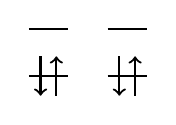
\begin{tikzpicture}
    % oberste MOs:
    \draw[thick] (0,0) -- (0.5,0); % erster Strich
    \draw[thick] (1,0) -- (1.5,0); % zweiter Strich
    % unterste MOs:
    \draw[thick] (0,-0.6) -- (0.5,-0.6); % dritter Strich
    \draw[thick] (1,-0.6) -- (1.5,-0.6); % vierter Strich
\draw[-> , thick] (0.35, -0.85) -- (0.35, -0.35); 
\draw[<- , thick] (0.15, -0.85) -- (0.15, -0.35); 
 \draw[-> , thick] (1.35, -0.85) -- (1.35, -0.35); 
\draw[<- , thick] (1.15, -0.85) -- (1.15, -0.35); 
\end{tikzpicture} \qquad 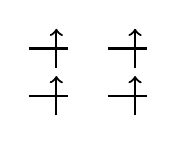
\begin{tikzpicture}
    % oberste MOs:
    \draw[thick] (0,0) -- (0.5,0); % erster Strich
    \draw[thick] (1,0) -- (1.5,0); % zweiter Strich
    % unterste MOs:
    \draw[thick] (0,-0.6) -- (0.5,-0.6); % dritter Strich
    \draw[thick] (1,-0.6) -- (1.5,-0.6); % vierter Strich
\draw[->, thick] (0.35, -0.25) -- (0.35, 0.25); 
\draw[->, thick] (1.35, -0.25) -- (1.35, 0.25); 
\draw[-> , thick] (0.35, -0.85) -- (0.35, -0.35); 
 \draw[-> , thick] (1.35, -0.85) -- (1.35, -0.35); 
\end{tikzpicture}\right)\]$$+\cdot \underbrace{(b_{1u}^{r})\cdot (a_{u}^{r})\cdot (b_{2g}^{r})\cdot (b_{3g}^{r})}_{\text{r: }a_{g}}\Rightarrow +\left|(b_{1u}^{r}) \cdot (b_{2g}^{r}) \cdot (b_{3g}^{r}) \cdot (a_{u}^{r})\right|$$$$=+\left|(-a_{g}+b_{1u}) \cdot (-b_{3u}+b_{2g}) \cdot (-b_{2u}+b_{3g}) \cdot (-b_{1g}+a_{u})\right|$$\begin{multline*}
=+\left|\underbrace{\overbrace{a_{g} b_{3u} b_{2u} b_{1g}}^{1 2 3 4}}_{a_{g}}\right|-\left|\underbrace{\overbrace{a_{g} b_{3u} b_{2u} a_{u}}^{1 2 3 8}}_{b_{1u}}\right|-\left|\underbrace{\overbrace{a_{g} b_{3u} b_{3g} b_{1g}}^{1 2 7 4}}_{b_{1u}}\right|+\left|\underbrace{\overbrace{a_{g} b_{3u} b_{3g} a_{u}}^{1 2 7 8}}_{a_{g}}\right|\\
-\left|\underbrace{\overbrace{a_{g} b_{2g} b_{2u} b_{1g}}^{1 6 3 4}}_{b_{1u}}\right|+\left|\underbrace{\overbrace{a_{g} b_{2g} b_{2u} a_{u}}^{1 6 3 8}}_{a_{g}}\right|+\left|\underbrace{\overbrace{a_{g} b_{2g} b_{3g} b_{1g}}^{1 6 7 4}}_{a_{g}}\right|-\left|\underbrace{\overbrace{a_{g} b_{2g} b_{3g} a_{u}}^{1 6 7 8}}_{b_{1u}}\right|\\
-\left|\underbrace{\overbrace{b_{1u} b_{3u} b_{2u} b_{1g}}^{5 2 3 4}}_{b_{1u}}\right|+\left|\underbrace{\overbrace{b_{1u} b_{3u} b_{2u} a_{u}}^{5 2 3 8}}_{a_{g}}\right|+\left|\underbrace{\overbrace{b_{1u} b_{3u} b_{3g} b_{1g}}^{5 2 7 4}}_{a_{g}}\right|-\left|\underbrace{\overbrace{b_{1u} b_{3u} b_{3g} a_{u}}^{5 2 7 8}}_{b_{1u}}\right|\\
+\left|\underbrace{\overbrace{b_{1u} b_{2g} b_{2u} b_{1g}}^{5 6 3 4}}_{a_{g}}\right|-\left|\underbrace{\overbrace{b_{1u} b_{2g} b_{2u} a_{u}}^{5 6 3 8}}_{b_{1u}}\right|-\left|\underbrace{\overbrace{b_{1u} b_{2g} b_{3g} b_{1g}}^{5 6 7 4}}_{b_{1u}}\right|+\left|\underbrace{\overbrace{b_{1u} b_{2g} b_{3g} a_{u}}^{5 6 7 8}}_{a_{g}}\right|
\end{multline*}\begin{multline*}
=+\left|\underbrace{\overbrace{a_{g} b_{3u} b_{2u} b_{1g}}^{1 2 3 4}}_{a_{g}}\right|-\left|\underbrace{\overbrace{a_{g} b_{3u} b_{2u} a_{u}}^{1 2 3 8}}_{b_{1u}}\right|+\left|\underbrace{\overbrace{a_{g} b_{3u} b_{1g} b_{3g}}^{1 2 4 7}}_{b_{1u}}\right|+\left|\underbrace{\overbrace{a_{g} b_{3u} b_{3g} a_{u}}^{1 2 7 8}}_{a_{g}}\right|\\
-\left|\underbrace{\overbrace{a_{g} b_{2u} b_{1g} b_{2g}}^{1 3 4 6}}_{b_{1u}}\right|-\left|\underbrace{\overbrace{a_{g} b_{2u} b_{2g} a_{u}}^{1 3 6 8}}_{a_{g}}\right|+\left|\underbrace{\overbrace{a_{g} b_{1g} b_{2g} b_{3g}}^{1 4 6 7}}_{a_{g}}\right|-\left|\underbrace{\overbrace{a_{g} b_{2g} b_{3g} a_{u}}^{1 6 7 8}}_{b_{1u}}\right|\\
+\left|\underbrace{\overbrace{b_{3u} b_{2u} b_{1g} b_{1u}}^{2 3 4 5}}_{b_{1u}}\right|+\left|\underbrace{\overbrace{b_{3u} b_{2u} b_{1u} a_{u}}^{2 3 5 8}}_{a_{g}}\right|-\left|\underbrace{\overbrace{b_{3u} b_{1g} b_{1u} b_{3g}}^{2 4 5 7}}_{a_{g}}\right|+\left|\underbrace{\overbrace{b_{3u} b_{1u} b_{3g} a_{u}}^{2 5 7 8}}_{b_{1u}}\right|\\
+\left|\underbrace{\overbrace{b_{2u} b_{1g} b_{1u} b_{2g}}^{3 4 5 6}}_{a_{g}}\right|-\left|\underbrace{\overbrace{b_{2u} b_{1u} b_{2g} a_{u}}^{3 5 6 8}}_{b_{1u}}\right|+\left|\underbrace{\overbrace{b_{1g} b_{1u} b_{2g} b_{3g}}^{4 5 6 7}}_{b_{1u}}\right|+\left|\underbrace{\overbrace{b_{1u} b_{2g} b_{3g} a_{u}}^{5 6 7 8}}_{a_{g}}\right|
\end{multline*}(nicht kürzbar)\\ \\
\hrule\newpage 


\[+\left(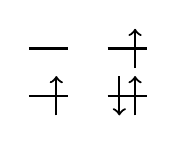
\begin{tikzpicture}
    % oberste MOs:
    \draw[thick] (0,0) -- (0.5,0); % erster Strich
    \draw[thick] (1,0) -- (1.5,0); % zweiter Strich
    % unterste MOs:
    \draw[thick] (0,-0.6) -- (0.5,-0.6); % dritter Strich
    \draw[thick] (1,-0.6) -- (1.5,-0.6); % vierter Strich
\draw[->, thick] (1.35, -0.25) -- (1.35, 0.25); 
\draw[-> , thick] (0.35, -0.85) -- (0.35, -0.35); 
 \draw[-> , thick] (1.35, -0.85) -- (1.35, -0.35); 
\draw[<- , thick] (1.15, -0.85) -- (1.15, -0.35); 
\end{tikzpicture} \qquad 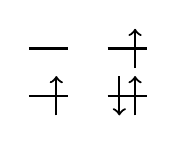
\begin{tikzpicture}
    % oberste MOs:
    \draw[thick] (0,0) -- (0.5,0); % erster Strich
    \draw[thick] (1,0) -- (1.5,0); % zweiter Strich
    % unterste MOs:
    \draw[thick] (0,-0.6) -- (0.5,-0.6); % dritter Strich
    \draw[thick] (1,-0.6) -- (1.5,-0.6); % vierter Strich
\draw[->, thick] (1.35, -0.25) -- (1.35, 0.25); 
\draw[-> , thick] (0.35, -0.85) -- (0.35, -0.35); 
 \draw[-> , thick] (1.35, -0.85) -- (1.35, -0.35); 
\draw[<- , thick] (1.15, -0.85) -- (1.15, -0.35); 
\end{tikzpicture}\right)\]$$+\cdot \underbrace{(a_{u}^{l})\cdot (b_{2g}^{l})}_{\text{l: }b_{2u}}\cdot \underbrace{(a_{u}^{r})\cdot (b_{2g}^{r})}_{\text{r: }b_{2u}}\Rightarrow +\left|(b_{2g}^{l}) \cdot (b_{2g}^{r}) \cdot (a_{u}^{l}) \cdot (a_{u}^{r})\right|$$$$=+\left|(+b_{3u}+b_{2g}) \cdot (-b_{3u}+b_{2g}) \cdot (+b_{1g}+a_{u}) \cdot (-b_{1g}+a_{u})\right|$$\begin{multline*}
=+\left|\underbrace{\overbrace{b_{3u} b_{2g} b_{1g} a_{u}}^{2 6 4 8}}_{a_{g}}\right|-\left|\underbrace{\overbrace{b_{3u} b_{2g} a_{u} b_{1g}}^{2 6 8 4}}_{a_{g}}\right|-\left|\underbrace{\overbrace{b_{2g} b_{3u} b_{1g} a_{u}}^{6 2 4 8}}_{a_{g}}\right|+\left|\underbrace{\overbrace{b_{2g} b_{3u} a_{u} b_{1g}}^{6 2 8 4}}_{a_{g}}\right|\\
\end{multline*}\begin{multline*}
=-\left|\underbrace{\overbrace{b_{3u} b_{1g} b_{2g} a_{u}}^{2 4 6 8}}_{a_{g}}\right|-\left|\underbrace{\overbrace{b_{3u} b_{1g} b_{2g} a_{u}}^{2 4 6 8}}_{a_{g}}\right|-\left|\underbrace{\overbrace{b_{3u} b_{1g} b_{2g} a_{u}}^{2 4 6 8}}_{a_{g}}\right|-\left|\underbrace{\overbrace{b_{3u} b_{1g} b_{2g} a_{u}}^{2 4 6 8}}_{a_{g}}\right|\\
\end{multline*}zusammengefasst:\begin{multline*}
=-4\left|\underbrace{\overbrace{b_{3u} b_{1g} b_{2g} a_{u}}^{2 4 6 8}}_{a_{g}}\right|
\end{multline*}\\ \\
\hrule\newpage 


\[+\left(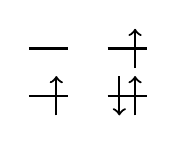
\begin{tikzpicture}
    % oberste MOs:
    \draw[thick] (0,0) -- (0.5,0); % erster Strich
    \draw[thick] (1,0) -- (1.5,0); % zweiter Strich
    % unterste MOs:
    \draw[thick] (0,-0.6) -- (0.5,-0.6); % dritter Strich
    \draw[thick] (1,-0.6) -- (1.5,-0.6); % vierter Strich
\draw[->, thick] (1.35, -0.25) -- (1.35, 0.25); 
\draw[-> , thick] (0.35, -0.85) -- (0.35, -0.35); 
 \draw[-> , thick] (1.35, -0.85) -- (1.35, -0.35); 
\draw[<- , thick] (1.15, -0.85) -- (1.15, -0.35); 
\end{tikzpicture} \qquad 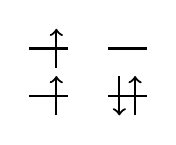
\begin{tikzpicture}
    % oberste MOs:
    \draw[thick] (0,0) -- (0.5,0); % erster Strich
    \draw[thick] (1,0) -- (1.5,0); % zweiter Strich
    % unterste MOs:
    \draw[thick] (0,-0.6) -- (0.5,-0.6); % dritter Strich
    \draw[thick] (1,-0.6) -- (1.5,-0.6); % vierter Strich
\draw[->, thick] (0.35, -0.25) -- (0.35, 0.25); 
\draw[-> , thick] (0.35, -0.85) -- (0.35, -0.35); 
 \draw[-> , thick] (1.35, -0.85) -- (1.35, -0.35); 
\draw[<- , thick] (1.15, -0.85) -- (1.15, -0.35); 
\end{tikzpicture}\right)\]$$+\cdot \underbrace{(a_{u}^{l})\cdot (b_{2g}^{l})}_{\text{l: }b_{2u}}\cdot \underbrace{(b_{1u}^{r})\cdot (b_{2g}^{r})}_{\text{r: }b_{3u}}\Rightarrow +\left|(b_{1u}^{r}) \cdot (b_{2g}^{l}) \cdot (b_{2g}^{r}) \cdot (a_{u}^{l})\right|$$$$=+\left|(-a_{g}+b_{1u}) \cdot (+b_{3u}+b_{2g}) \cdot (-b_{3u}+b_{2g}) \cdot (+b_{1g}+a_{u})\right|$$\begin{multline*}
=-\left|\underbrace{\overbrace{a_{g} b_{3u} b_{2g} b_{1g}}^{1 2 6 4}}_{a_{u}}\right|-\left|\underbrace{\overbrace{a_{g} b_{3u} b_{2g} a_{u}}^{1 2 6 8}}_{b_{1g}}\right|+\left|\underbrace{\overbrace{a_{g} b_{2g} b_{3u} b_{1g}}^{1 6 2 4}}_{a_{u}}\right|+\left|\underbrace{\overbrace{a_{g} b_{2g} b_{3u} a_{u}}^{1 6 2 8}}_{b_{1g}}\right|\\
+\left|\underbrace{\overbrace{b_{1u} b_{3u} b_{2g} b_{1g}}^{5 2 6 4}}_{b_{1g}}\right|+\left|\underbrace{\overbrace{b_{1u} b_{3u} b_{2g} a_{u}}^{5 2 6 8}}_{a_{u}}\right|-\left|\underbrace{\overbrace{b_{1u} b_{2g} b_{3u} b_{1g}}^{5 6 2 4}}_{b_{1g}}\right|-\left|\underbrace{\overbrace{b_{1u} b_{2g} b_{3u} a_{u}}^{5 6 2 8}}_{a_{u}}\right|\\
\end{multline*}\begin{multline*}
=+\left|\underbrace{\overbrace{a_{g} b_{3u} b_{1g} b_{2g}}^{1 2 4 6}}_{a_{u}}\right|-\left|\underbrace{\overbrace{a_{g} b_{3u} b_{2g} a_{u}}^{1 2 6 8}}_{b_{1g}}\right|+\left|\underbrace{\overbrace{a_{g} b_{3u} b_{1g} b_{2g}}^{1 2 4 6}}_{a_{u}}\right|-\left|\underbrace{\overbrace{a_{g} b_{3u} b_{2g} a_{u}}^{1 2 6 8}}_{b_{1g}}\right|\\
-\left|\underbrace{\overbrace{b_{3u} b_{1g} b_{1u} b_{2g}}^{2 4 5 6}}_{b_{1g}}\right|-\left|\underbrace{\overbrace{b_{3u} b_{1u} b_{2g} a_{u}}^{2 5 6 8}}_{a_{u}}\right|-\left|\underbrace{\overbrace{b_{3u} b_{1g} b_{1u} b_{2g}}^{2 4 5 6}}_{b_{1g}}\right|-\left|\underbrace{\overbrace{b_{3u} b_{1u} b_{2g} a_{u}}^{2 5 6 8}}_{a_{u}}\right|\\
\end{multline*}zusammengefasst:\begin{multline*}
=+2\left|\underbrace{\overbrace{a_{g} b_{3u} b_{1g} b_{2g}}^{1 2 4 6}}_{a_{u}}\right|-2\left|\underbrace{\overbrace{a_{g} b_{3u} b_{2g} a_{u}}^{1 2 6 8}}_{b_{1g}}\right|-2\left|\underbrace{\overbrace{b_{3u} b_{1g} b_{1u} b_{2g}}^{2 4 5 6}}_{b_{1g}}\right|-2\left|\underbrace{\overbrace{b_{3u} b_{1u} b_{2g} a_{u}}^{2 5 6 8}}_{a_{u}}\right|\\
\end{multline*}\\ \\
\vspace{0.5cm}

\[+\left(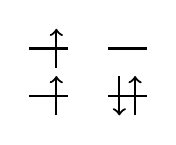
\begin{tikzpicture}
    % oberste MOs:
    \draw[thick] (0,0) -- (0.5,0); % erster Strich
    \draw[thick] (1,0) -- (1.5,0); % zweiter Strich
    % unterste MOs:
    \draw[thick] (0,-0.6) -- (0.5,-0.6); % dritter Strich
    \draw[thick] (1,-0.6) -- (1.5,-0.6); % vierter Strich
\draw[->, thick] (0.35, -0.25) -- (0.35, 0.25); 
\draw[-> , thick] (0.35, -0.85) -- (0.35, -0.35); 
 \draw[-> , thick] (1.35, -0.85) -- (1.35, -0.35); 
\draw[<- , thick] (1.15, -0.85) -- (1.15, -0.35); 
\end{tikzpicture} \qquad 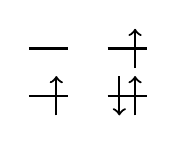
\begin{tikzpicture}
    % oberste MOs:
    \draw[thick] (0,0) -- (0.5,0); % erster Strich
    \draw[thick] (1,0) -- (1.5,0); % zweiter Strich
    % unterste MOs:
    \draw[thick] (0,-0.6) -- (0.5,-0.6); % dritter Strich
    \draw[thick] (1,-0.6) -- (1.5,-0.6); % vierter Strich
\draw[->, thick] (1.35, -0.25) -- (1.35, 0.25); 
\draw[-> , thick] (0.35, -0.85) -- (0.35, -0.35); 
 \draw[-> , thick] (1.35, -0.85) -- (1.35, -0.35); 
\draw[<- , thick] (1.15, -0.85) -- (1.15, -0.35); 
\end{tikzpicture}\right)\]$$+\cdot \underbrace{(b_{1u}^{l})\cdot (b_{2g}^{l})}_{\text{l: }b_{3u}}\cdot \underbrace{(a_{u}^{r})\cdot (b_{2g}^{r})}_{\text{r: }b_{2u}}\Rightarrow +\left|(b_{1u}^{l}) \cdot (b_{2g}^{l}) \cdot (b_{2g}^{r}) \cdot (a_{u}^{r})\right|$$$$=+\left|(+a_{g}+b_{1u}) \cdot (+b_{3u}+b_{2g}) \cdot (-b_{3u}+b_{2g}) \cdot (-b_{1g}+a_{u})\right|$$\begin{multline*}
=-\left|\underbrace{\overbrace{a_{g} b_{3u} b_{2g} b_{1g}}^{1 2 6 4}}_{a_{u}}\right|+\left|\underbrace{\overbrace{a_{g} b_{3u} b_{2g} a_{u}}^{1 2 6 8}}_{b_{1g}}\right|+\left|\underbrace{\overbrace{a_{g} b_{2g} b_{3u} b_{1g}}^{1 6 2 4}}_{a_{u}}\right|-\left|\underbrace{\overbrace{a_{g} b_{2g} b_{3u} a_{u}}^{1 6 2 8}}_{b_{1g}}\right|\\
-\left|\underbrace{\overbrace{b_{1u} b_{3u} b_{2g} b_{1g}}^{5 2 6 4}}_{b_{1g}}\right|+\left|\underbrace{\overbrace{b_{1u} b_{3u} b_{2g} a_{u}}^{5 2 6 8}}_{a_{u}}\right|+\left|\underbrace{\overbrace{b_{1u} b_{2g} b_{3u} b_{1g}}^{5 6 2 4}}_{b_{1g}}\right|-\left|\underbrace{\overbrace{b_{1u} b_{2g} b_{3u} a_{u}}^{5 6 2 8}}_{a_{u}}\right|\\
\end{multline*}\begin{multline*}
=+\left|\underbrace{\overbrace{a_{g} b_{3u} b_{1g} b_{2g}}^{1 2 4 6}}_{a_{u}}\right|+\left|\underbrace{\overbrace{a_{g} b_{3u} b_{2g} a_{u}}^{1 2 6 8}}_{b_{1g}}\right|+\left|\underbrace{\overbrace{a_{g} b_{3u} b_{1g} b_{2g}}^{1 2 4 6}}_{a_{u}}\right|+\left|\underbrace{\overbrace{a_{g} b_{3u} b_{2g} a_{u}}^{1 2 6 8}}_{b_{1g}}\right|\\
+\left|\underbrace{\overbrace{b_{3u} b_{1g} b_{1u} b_{2g}}^{2 4 5 6}}_{b_{1g}}\right|-\left|\underbrace{\overbrace{b_{3u} b_{1u} b_{2g} a_{u}}^{2 5 6 8}}_{a_{u}}\right|+\left|\underbrace{\overbrace{b_{3u} b_{1g} b_{1u} b_{2g}}^{2 4 5 6}}_{b_{1g}}\right|-\left|\underbrace{\overbrace{b_{3u} b_{1u} b_{2g} a_{u}}^{2 5 6 8}}_{a_{u}}\right|\\
\end{multline*}zusammengefasst:\begin{multline*}
=+2\left|\underbrace{\overbrace{a_{g} b_{3u} b_{1g} b_{2g}}^{1 2 4 6}}_{a_{u}}\right|+2\left|\underbrace{\overbrace{a_{g} b_{3u} b_{2g} a_{u}}^{1 2 6 8}}_{b_{1g}}\right|+2\left|\underbrace{\overbrace{b_{3u} b_{1g} b_{1u} b_{2g}}^{2 4 5 6}}_{b_{1g}}\right|-2\left|\underbrace{\overbrace{b_{3u} b_{1u} b_{2g} a_{u}}^{2 5 6 8}}_{a_{u}}\right|\\
\end{multline*}\\ \\
\hrule\newpage 


\[+\left(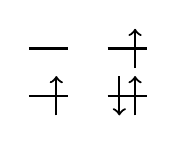
\begin{tikzpicture}
    % oberste MOs:
    \draw[thick] (0,0) -- (0.5,0); % erster Strich
    \draw[thick] (1,0) -- (1.5,0); % zweiter Strich
    % unterste MOs:
    \draw[thick] (0,-0.6) -- (0.5,-0.6); % dritter Strich
    \draw[thick] (1,-0.6) -- (1.5,-0.6); % vierter Strich
\draw[->, thick] (1.35, -0.25) -- (1.35, 0.25); 
\draw[-> , thick] (0.35, -0.85) -- (0.35, -0.35); 
 \draw[-> , thick] (1.35, -0.85) -- (1.35, -0.35); 
\draw[<- , thick] (1.15, -0.85) -- (1.15, -0.35); 
\end{tikzpicture} \qquad 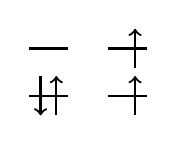
\begin{tikzpicture}
    % oberste MOs:
    \draw[thick] (0,0) -- (0.5,0); % erster Strich
    \draw[thick] (1,0) -- (1.5,0); % zweiter Strich
    % unterste MOs:
    \draw[thick] (0,-0.6) -- (0.5,-0.6); % dritter Strich
    \draw[thick] (1,-0.6) -- (1.5,-0.6); % vierter Strich
\draw[->, thick] (1.35, -0.25) -- (1.35, 0.25); 
\draw[-> , thick] (0.35, -0.85) -- (0.35, -0.35); 
\draw[<- , thick] (0.15, -0.85) -- (0.15, -0.35); 
 \draw[-> , thick] (1.35, -0.85) -- (1.35, -0.35); 
\end{tikzpicture}\right)\]$$+\cdot \underbrace{(a_{u}^{l})\cdot (b_{2g}^{l})}_{\text{l: }b_{2u}}\cdot \underbrace{(a_{u}^{r})\cdot (b_{3g}^{r})}_{\text{r: }b_{3u}}\Rightarrow +\left|(b_{2g}^{l}) \cdot (b_{3g}^{r}) \cdot (a_{u}^{l}) \cdot (a_{u}^{r})\right|$$$$=+\left|(+b_{3u}+b_{2g}) \cdot (-b_{2u}+b_{3g}) \cdot (+b_{1g}+a_{u}) \cdot (-b_{1g}+a_{u})\right|$$\begin{multline*}
=-\left|\underbrace{\overbrace{b_{3u} b_{2u} b_{1g} a_{u}}^{2 3 4 8}}_{a_{u}}\right|+\left|\underbrace{\overbrace{b_{3u} b_{2u} a_{u} b_{1g}}^{2 3 8 4}}_{a_{u}}\right|+\left|\underbrace{\overbrace{b_{3u} b_{3g} b_{1g} a_{u}}^{2 7 4 8}}_{b_{1g}}\right|-\left|\underbrace{\overbrace{b_{3u} b_{3g} a_{u} b_{1g}}^{2 7 8 4}}_{b_{1g}}\right|\\
-\left|\underbrace{\overbrace{b_{2g} b_{2u} b_{1g} a_{u}}^{6 3 4 8}}_{b_{1g}}\right|+\left|\underbrace{\overbrace{b_{2g} b_{2u} a_{u} b_{1g}}^{6 3 8 4}}_{b_{1g}}\right|+\left|\underbrace{\overbrace{b_{2g} b_{3g} b_{1g} a_{u}}^{6 7 4 8}}_{a_{u}}\right|-\left|\underbrace{\overbrace{b_{2g} b_{3g} a_{u} b_{1g}}^{6 7 8 4}}_{a_{u}}\right|\\
\end{multline*}\begin{multline*}
=-\left|\underbrace{\overbrace{b_{3u} b_{2u} b_{1g} a_{u}}^{2 3 4 8}}_{a_{u}}\right|-\left|\underbrace{\overbrace{b_{3u} b_{2u} b_{1g} a_{u}}^{2 3 4 8}}_{a_{u}}\right|-\left|\underbrace{\overbrace{b_{3u} b_{1g} b_{3g} a_{u}}^{2 4 7 8}}_{b_{1g}}\right|-\left|\underbrace{\overbrace{b_{3u} b_{1g} b_{3g} a_{u}}^{2 4 7 8}}_{b_{1g}}\right|\\
-\left|\underbrace{\overbrace{b_{2u} b_{1g} b_{2g} a_{u}}^{3 4 6 8}}_{b_{1g}}\right|-\left|\underbrace{\overbrace{b_{2u} b_{1g} b_{2g} a_{u}}^{3 4 6 8}}_{b_{1g}}\right|+\left|\underbrace{\overbrace{b_{1g} b_{2g} b_{3g} a_{u}}^{4 6 7 8}}_{a_{u}}\right|+\left|\underbrace{\overbrace{b_{1g} b_{2g} b_{3g} a_{u}}^{4 6 7 8}}_{a_{u}}\right|\\
\end{multline*}zusammengefasst:\begin{multline*}
=-2\left|\underbrace{\overbrace{b_{3u} b_{2u} b_{1g} a_{u}}^{2 3 4 8}}_{a_{u}}\right|-2\left|\underbrace{\overbrace{b_{3u} b_{1g} b_{3g} a_{u}}^{2 4 7 8}}_{b_{1g}}\right|-2\left|\underbrace{\overbrace{b_{2u} b_{1g} b_{2g} a_{u}}^{3 4 6 8}}_{b_{1g}}\right|+2\left|\underbrace{\overbrace{b_{1g} b_{2g} b_{3g} a_{u}}^{4 6 7 8}}_{a_{u}}\right|\\
\end{multline*}\\ \\
\vspace{0.5cm}

\[+\left(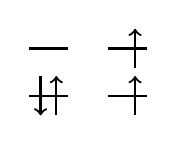
\begin{tikzpicture}
    % oberste MOs:
    \draw[thick] (0,0) -- (0.5,0); % erster Strich
    \draw[thick] (1,0) -- (1.5,0); % zweiter Strich
    % unterste MOs:
    \draw[thick] (0,-0.6) -- (0.5,-0.6); % dritter Strich
    \draw[thick] (1,-0.6) -- (1.5,-0.6); % vierter Strich
\draw[->, thick] (1.35, -0.25) -- (1.35, 0.25); 
\draw[-> , thick] (0.35, -0.85) -- (0.35, -0.35); 
\draw[<- , thick] (0.15, -0.85) -- (0.15, -0.35); 
 \draw[-> , thick] (1.35, -0.85) -- (1.35, -0.35); 
\end{tikzpicture} \qquad 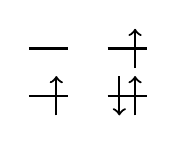
\begin{tikzpicture}
    % oberste MOs:
    \draw[thick] (0,0) -- (0.5,0); % erster Strich
    \draw[thick] (1,0) -- (1.5,0); % zweiter Strich
    % unterste MOs:
    \draw[thick] (0,-0.6) -- (0.5,-0.6); % dritter Strich
    \draw[thick] (1,-0.6) -- (1.5,-0.6); % vierter Strich
\draw[->, thick] (1.35, -0.25) -- (1.35, 0.25); 
\draw[-> , thick] (0.35, -0.85) -- (0.35, -0.35); 
 \draw[-> , thick] (1.35, -0.85) -- (1.35, -0.35); 
\draw[<- , thick] (1.15, -0.85) -- (1.15, -0.35); 
\end{tikzpicture}\right)\]$$+\cdot \underbrace{(a_{u}^{l})\cdot (b_{3g}^{l})}_{\text{l: }b_{3u}}\cdot \underbrace{(a_{u}^{r})\cdot (b_{2g}^{r})}_{\text{r: }b_{2u}}\Rightarrow +\left|(b_{2g}^{r}) \cdot (b_{3g}^{l}) \cdot (a_{u}^{l}) \cdot (a_{u}^{r})\right|$$$$=+\left|(-b_{3u}+b_{2g}) \cdot (+b_{2u}+b_{3g}) \cdot (+b_{1g}+a_{u}) \cdot (-b_{1g}+a_{u})\right|$$\begin{multline*}
=-\left|\underbrace{\overbrace{b_{3u} b_{2u} b_{1g} a_{u}}^{2 3 4 8}}_{a_{u}}\right|+\left|\underbrace{\overbrace{b_{3u} b_{2u} a_{u} b_{1g}}^{2 3 8 4}}_{a_{u}}\right|-\left|\underbrace{\overbrace{b_{3u} b_{3g} b_{1g} a_{u}}^{2 7 4 8}}_{b_{1g}}\right|+\left|\underbrace{\overbrace{b_{3u} b_{3g} a_{u} b_{1g}}^{2 7 8 4}}_{b_{1g}}\right|\\
+\left|\underbrace{\overbrace{b_{2g} b_{2u} b_{1g} a_{u}}^{6 3 4 8}}_{b_{1g}}\right|-\left|\underbrace{\overbrace{b_{2g} b_{2u} a_{u} b_{1g}}^{6 3 8 4}}_{b_{1g}}\right|+\left|\underbrace{\overbrace{b_{2g} b_{3g} b_{1g} a_{u}}^{6 7 4 8}}_{a_{u}}\right|-\left|\underbrace{\overbrace{b_{2g} b_{3g} a_{u} b_{1g}}^{6 7 8 4}}_{a_{u}}\right|\\
\end{multline*}\begin{multline*}
=-\left|\underbrace{\overbrace{b_{3u} b_{2u} b_{1g} a_{u}}^{2 3 4 8}}_{a_{u}}\right|-\left|\underbrace{\overbrace{b_{3u} b_{2u} b_{1g} a_{u}}^{2 3 4 8}}_{a_{u}}\right|+\left|\underbrace{\overbrace{b_{3u} b_{1g} b_{3g} a_{u}}^{2 4 7 8}}_{b_{1g}}\right|+\left|\underbrace{\overbrace{b_{3u} b_{1g} b_{3g} a_{u}}^{2 4 7 8}}_{b_{1g}}\right|\\
+\left|\underbrace{\overbrace{b_{2u} b_{1g} b_{2g} a_{u}}^{3 4 6 8}}_{b_{1g}}\right|+\left|\underbrace{\overbrace{b_{2u} b_{1g} b_{2g} a_{u}}^{3 4 6 8}}_{b_{1g}}\right|+\left|\underbrace{\overbrace{b_{1g} b_{2g} b_{3g} a_{u}}^{4 6 7 8}}_{a_{u}}\right|+\left|\underbrace{\overbrace{b_{1g} b_{2g} b_{3g} a_{u}}^{4 6 7 8}}_{a_{u}}\right|\\
\end{multline*}zusammengefasst:\begin{multline*}
=-2\left|\underbrace{\overbrace{b_{3u} b_{2u} b_{1g} a_{u}}^{2 3 4 8}}_{a_{u}}\right|+2\left|\underbrace{\overbrace{b_{3u} b_{1g} b_{3g} a_{u}}^{2 4 7 8}}_{b_{1g}}\right|+2\left|\underbrace{\overbrace{b_{2u} b_{1g} b_{2g} a_{u}}^{3 4 6 8}}_{b_{1g}}\right|+2\left|\underbrace{\overbrace{b_{1g} b_{2g} b_{3g} a_{u}}^{4 6 7 8}}_{a_{u}}\right|\\
\end{multline*}\\ \\
\hrule\newpage 


\[+\left(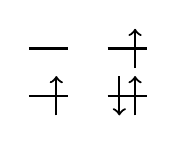
\begin{tikzpicture}
    % oberste MOs:
    \draw[thick] (0,0) -- (0.5,0); % erster Strich
    \draw[thick] (1,0) -- (1.5,0); % zweiter Strich
    % unterste MOs:
    \draw[thick] (0,-0.6) -- (0.5,-0.6); % dritter Strich
    \draw[thick] (1,-0.6) -- (1.5,-0.6); % vierter Strich
\draw[->, thick] (1.35, -0.25) -- (1.35, 0.25); 
\draw[-> , thick] (0.35, -0.85) -- (0.35, -0.35); 
 \draw[-> , thick] (1.35, -0.85) -- (1.35, -0.35); 
\draw[<- , thick] (1.15, -0.85) -- (1.15, -0.35); 
\end{tikzpicture} \qquad 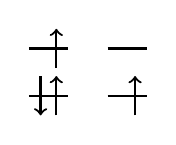
\begin{tikzpicture}
    % oberste MOs:
    \draw[thick] (0,0) -- (0.5,0); % erster Strich
    \draw[thick] (1,0) -- (1.5,0); % zweiter Strich
    % unterste MOs:
    \draw[thick] (0,-0.6) -- (0.5,-0.6); % dritter Strich
    \draw[thick] (1,-0.6) -- (1.5,-0.6); % vierter Strich
\draw[->, thick] (0.35, -0.25) -- (0.35, 0.25); 
\draw[-> , thick] (0.35, -0.85) -- (0.35, -0.35); 
\draw[<- , thick] (0.15, -0.85) -- (0.15, -0.35); 
 \draw[-> , thick] (1.35, -0.85) -- (1.35, -0.35); 
\end{tikzpicture}\right)\]$$+\cdot \underbrace{(a_{u}^{l})\cdot (b_{2g}^{l})}_{\text{l: }b_{2u}}\cdot \underbrace{(b_{1u}^{r})\cdot (b_{3g}^{r})}_{\text{r: }b_{2u}}\Rightarrow +\left|(b_{1u}^{r}) \cdot (b_{2g}^{l}) \cdot (b_{3g}^{r}) \cdot (a_{u}^{l})\right|$$$$=+\left|(-a_{g}+b_{1u}) \cdot (+b_{3u}+b_{2g}) \cdot (-b_{2u}+b_{3g}) \cdot (+b_{1g}+a_{u})\right|$$\begin{multline*}
=+\left|\underbrace{\overbrace{a_{g} b_{3u} b_{2u} b_{1g}}^{1 2 3 4}}_{a_{g}}\right|+\left|\underbrace{\overbrace{a_{g} b_{3u} b_{2u} a_{u}}^{1 2 3 8}}_{b_{1u}}\right|-\left|\underbrace{\overbrace{a_{g} b_{3u} b_{3g} b_{1g}}^{1 2 7 4}}_{b_{1u}}\right|-\left|\underbrace{\overbrace{a_{g} b_{3u} b_{3g} a_{u}}^{1 2 7 8}}_{a_{g}}\right|\\
+\left|\underbrace{\overbrace{a_{g} b_{2g} b_{2u} b_{1g}}^{1 6 3 4}}_{b_{1u}}\right|+\left|\underbrace{\overbrace{a_{g} b_{2g} b_{2u} a_{u}}^{1 6 3 8}}_{a_{g}}\right|-\left|\underbrace{\overbrace{a_{g} b_{2g} b_{3g} b_{1g}}^{1 6 7 4}}_{a_{g}}\right|-\left|\underbrace{\overbrace{a_{g} b_{2g} b_{3g} a_{u}}^{1 6 7 8}}_{b_{1u}}\right|\\
-\left|\underbrace{\overbrace{b_{1u} b_{3u} b_{2u} b_{1g}}^{5 2 3 4}}_{b_{1u}}\right|-\left|\underbrace{\overbrace{b_{1u} b_{3u} b_{2u} a_{u}}^{5 2 3 8}}_{a_{g}}\right|+\left|\underbrace{\overbrace{b_{1u} b_{3u} b_{3g} b_{1g}}^{5 2 7 4}}_{a_{g}}\right|+\left|\underbrace{\overbrace{b_{1u} b_{3u} b_{3g} a_{u}}^{5 2 7 8}}_{b_{1u}}\right|\\
-\left|\underbrace{\overbrace{b_{1u} b_{2g} b_{2u} b_{1g}}^{5 6 3 4}}_{a_{g}}\right|-\left|\underbrace{\overbrace{b_{1u} b_{2g} b_{2u} a_{u}}^{5 6 3 8}}_{b_{1u}}\right|+\left|\underbrace{\overbrace{b_{1u} b_{2g} b_{3g} b_{1g}}^{5 6 7 4}}_{b_{1u}}\right|+\left|\underbrace{\overbrace{b_{1u} b_{2g} b_{3g} a_{u}}^{5 6 7 8}}_{a_{g}}\right|
\end{multline*}\begin{multline*}
=+\left|\underbrace{\overbrace{a_{g} b_{3u} b_{2u} b_{1g}}^{1 2 3 4}}_{a_{g}}\right|+\left|\underbrace{\overbrace{a_{g} b_{3u} b_{2u} a_{u}}^{1 2 3 8}}_{b_{1u}}\right|+\left|\underbrace{\overbrace{a_{g} b_{3u} b_{1g} b_{3g}}^{1 2 4 7}}_{b_{1u}}\right|-\left|\underbrace{\overbrace{a_{g} b_{3u} b_{3g} a_{u}}^{1 2 7 8}}_{a_{g}}\right|\\
+\left|\underbrace{\overbrace{a_{g} b_{2u} b_{1g} b_{2g}}^{1 3 4 6}}_{b_{1u}}\right|-\left|\underbrace{\overbrace{a_{g} b_{2u} b_{2g} a_{u}}^{1 3 6 8}}_{a_{g}}\right|-\left|\underbrace{\overbrace{a_{g} b_{1g} b_{2g} b_{3g}}^{1 4 6 7}}_{a_{g}}\right|-\left|\underbrace{\overbrace{a_{g} b_{2g} b_{3g} a_{u}}^{1 6 7 8}}_{b_{1u}}\right|\\
+\left|\underbrace{\overbrace{b_{3u} b_{2u} b_{1g} b_{1u}}^{2 3 4 5}}_{b_{1u}}\right|-\left|\underbrace{\overbrace{b_{3u} b_{2u} b_{1u} a_{u}}^{2 3 5 8}}_{a_{g}}\right|-\left|\underbrace{\overbrace{b_{3u} b_{1g} b_{1u} b_{3g}}^{2 4 5 7}}_{a_{g}}\right|-\left|\underbrace{\overbrace{b_{3u} b_{1u} b_{3g} a_{u}}^{2 5 7 8}}_{b_{1u}}\right|\\
-\left|\underbrace{\overbrace{b_{2u} b_{1g} b_{1u} b_{2g}}^{3 4 5 6}}_{a_{g}}\right|-\left|\underbrace{\overbrace{b_{2u} b_{1u} b_{2g} a_{u}}^{3 5 6 8}}_{b_{1u}}\right|-\left|\underbrace{\overbrace{b_{1g} b_{1u} b_{2g} b_{3g}}^{4 5 6 7}}_{b_{1u}}\right|+\left|\underbrace{\overbrace{b_{1u} b_{2g} b_{3g} a_{u}}^{5 6 7 8}}_{a_{g}}\right|
\end{multline*}(nicht kürzbar)\\ \\
\vspace{0.5cm}

\[+\left(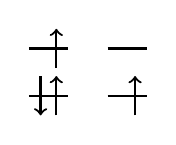
\begin{tikzpicture}
    % oberste MOs:
    \draw[thick] (0,0) -- (0.5,0); % erster Strich
    \draw[thick] (1,0) -- (1.5,0); % zweiter Strich
    % unterste MOs:
    \draw[thick] (0,-0.6) -- (0.5,-0.6); % dritter Strich
    \draw[thick] (1,-0.6) -- (1.5,-0.6); % vierter Strich
\draw[->, thick] (0.35, -0.25) -- (0.35, 0.25); 
\draw[-> , thick] (0.35, -0.85) -- (0.35, -0.35); 
\draw[<- , thick] (0.15, -0.85) -- (0.15, -0.35); 
 \draw[-> , thick] (1.35, -0.85) -- (1.35, -0.35); 
\end{tikzpicture} \qquad 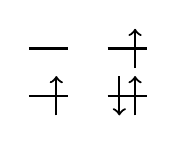
\begin{tikzpicture}
    % oberste MOs:
    \draw[thick] (0,0) -- (0.5,0); % erster Strich
    \draw[thick] (1,0) -- (1.5,0); % zweiter Strich
    % unterste MOs:
    \draw[thick] (0,-0.6) -- (0.5,-0.6); % dritter Strich
    \draw[thick] (1,-0.6) -- (1.5,-0.6); % vierter Strich
\draw[->, thick] (1.35, -0.25) -- (1.35, 0.25); 
\draw[-> , thick] (0.35, -0.85) -- (0.35, -0.35); 
 \draw[-> , thick] (1.35, -0.85) -- (1.35, -0.35); 
\draw[<- , thick] (1.15, -0.85) -- (1.15, -0.35); 
\end{tikzpicture}\right)\]$$+\cdot \underbrace{(b_{1u}^{l})\cdot (b_{3g}^{l})}_{\text{l: }b_{2u}}\cdot \underbrace{(a_{u}^{r})\cdot (b_{2g}^{r})}_{\text{r: }b_{2u}}\Rightarrow +\left|(b_{1u}^{l}) \cdot (b_{2g}^{r}) \cdot (b_{3g}^{l}) \cdot (a_{u}^{r})\right|$$$$=+\left|(+a_{g}+b_{1u}) \cdot (-b_{3u}+b_{2g}) \cdot (+b_{2u}+b_{3g}) \cdot (-b_{1g}+a_{u})\right|$$\begin{multline*}
=+\left|\underbrace{\overbrace{a_{g} b_{3u} b_{2u} b_{1g}}^{1 2 3 4}}_{a_{g}}\right|-\left|\underbrace{\overbrace{a_{g} b_{3u} b_{2u} a_{u}}^{1 2 3 8}}_{b_{1u}}\right|+\left|\underbrace{\overbrace{a_{g} b_{3u} b_{3g} b_{1g}}^{1 2 7 4}}_{b_{1u}}\right|-\left|\underbrace{\overbrace{a_{g} b_{3u} b_{3g} a_{u}}^{1 2 7 8}}_{a_{g}}\right|\\
-\left|\underbrace{\overbrace{a_{g} b_{2g} b_{2u} b_{1g}}^{1 6 3 4}}_{b_{1u}}\right|+\left|\underbrace{\overbrace{a_{g} b_{2g} b_{2u} a_{u}}^{1 6 3 8}}_{a_{g}}\right|-\left|\underbrace{\overbrace{a_{g} b_{2g} b_{3g} b_{1g}}^{1 6 7 4}}_{a_{g}}\right|+\left|\underbrace{\overbrace{a_{g} b_{2g} b_{3g} a_{u}}^{1 6 7 8}}_{b_{1u}}\right|\\
+\left|\underbrace{\overbrace{b_{1u} b_{3u} b_{2u} b_{1g}}^{5 2 3 4}}_{b_{1u}}\right|-\left|\underbrace{\overbrace{b_{1u} b_{3u} b_{2u} a_{u}}^{5 2 3 8}}_{a_{g}}\right|+\left|\underbrace{\overbrace{b_{1u} b_{3u} b_{3g} b_{1g}}^{5 2 7 4}}_{a_{g}}\right|-\left|\underbrace{\overbrace{b_{1u} b_{3u} b_{3g} a_{u}}^{5 2 7 8}}_{b_{1u}}\right|\\
-\left|\underbrace{\overbrace{b_{1u} b_{2g} b_{2u} b_{1g}}^{5 6 3 4}}_{a_{g}}\right|+\left|\underbrace{\overbrace{b_{1u} b_{2g} b_{2u} a_{u}}^{5 6 3 8}}_{b_{1u}}\right|-\left|\underbrace{\overbrace{b_{1u} b_{2g} b_{3g} b_{1g}}^{5 6 7 4}}_{b_{1u}}\right|+\left|\underbrace{\overbrace{b_{1u} b_{2g} b_{3g} a_{u}}^{5 6 7 8}}_{a_{g}}\right|
\end{multline*}\begin{multline*}
=+\left|\underbrace{\overbrace{a_{g} b_{3u} b_{2u} b_{1g}}^{1 2 3 4}}_{a_{g}}\right|-\left|\underbrace{\overbrace{a_{g} b_{3u} b_{2u} a_{u}}^{1 2 3 8}}_{b_{1u}}\right|-\left|\underbrace{\overbrace{a_{g} b_{3u} b_{1g} b_{3g}}^{1 2 4 7}}_{b_{1u}}\right|-\left|\underbrace{\overbrace{a_{g} b_{3u} b_{3g} a_{u}}^{1 2 7 8}}_{a_{g}}\right|\\
-\left|\underbrace{\overbrace{a_{g} b_{2u} b_{1g} b_{2g}}^{1 3 4 6}}_{b_{1u}}\right|-\left|\underbrace{\overbrace{a_{g} b_{2u} b_{2g} a_{u}}^{1 3 6 8}}_{a_{g}}\right|-\left|\underbrace{\overbrace{a_{g} b_{1g} b_{2g} b_{3g}}^{1 4 6 7}}_{a_{g}}\right|+\left|\underbrace{\overbrace{a_{g} b_{2g} b_{3g} a_{u}}^{1 6 7 8}}_{b_{1u}}\right|\\
-\left|\underbrace{\overbrace{b_{3u} b_{2u} b_{1g} b_{1u}}^{2 3 4 5}}_{b_{1u}}\right|-\left|\underbrace{\overbrace{b_{3u} b_{2u} b_{1u} a_{u}}^{2 3 5 8}}_{a_{g}}\right|-\left|\underbrace{\overbrace{b_{3u} b_{1g} b_{1u} b_{3g}}^{2 4 5 7}}_{a_{g}}\right|+\left|\underbrace{\overbrace{b_{3u} b_{1u} b_{3g} a_{u}}^{2 5 7 8}}_{b_{1u}}\right|\\
-\left|\underbrace{\overbrace{b_{2u} b_{1g} b_{1u} b_{2g}}^{3 4 5 6}}_{a_{g}}\right|+\left|\underbrace{\overbrace{b_{2u} b_{1u} b_{2g} a_{u}}^{3 5 6 8}}_{b_{1u}}\right|+\left|\underbrace{\overbrace{b_{1g} b_{1u} b_{2g} b_{3g}}^{4 5 6 7}}_{b_{1u}}\right|+\left|\underbrace{\overbrace{b_{1u} b_{2g} b_{3g} a_{u}}^{5 6 7 8}}_{a_{g}}\right|
\end{multline*}(nicht kürzbar)\\ \\
\hrule\newpage 


\[+\left(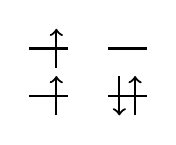
\begin{tikzpicture}
    % oberste MOs:
    \draw[thick] (0,0) -- (0.5,0); % erster Strich
    \draw[thick] (1,0) -- (1.5,0); % zweiter Strich
    % unterste MOs:
    \draw[thick] (0,-0.6) -- (0.5,-0.6); % dritter Strich
    \draw[thick] (1,-0.6) -- (1.5,-0.6); % vierter Strich
\draw[->, thick] (0.35, -0.25) -- (0.35, 0.25); 
\draw[-> , thick] (0.35, -0.85) -- (0.35, -0.35); 
 \draw[-> , thick] (1.35, -0.85) -- (1.35, -0.35); 
\draw[<- , thick] (1.15, -0.85) -- (1.15, -0.35); 
\end{tikzpicture} \qquad 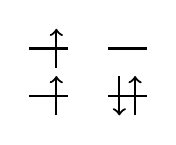
\begin{tikzpicture}
    % oberste MOs:
    \draw[thick] (0,0) -- (0.5,0); % erster Strich
    \draw[thick] (1,0) -- (1.5,0); % zweiter Strich
    % unterste MOs:
    \draw[thick] (0,-0.6) -- (0.5,-0.6); % dritter Strich
    \draw[thick] (1,-0.6) -- (1.5,-0.6); % vierter Strich
\draw[->, thick] (0.35, -0.25) -- (0.35, 0.25); 
\draw[-> , thick] (0.35, -0.85) -- (0.35, -0.35); 
 \draw[-> , thick] (1.35, -0.85) -- (1.35, -0.35); 
\draw[<- , thick] (1.15, -0.85) -- (1.15, -0.35); 
\end{tikzpicture}\right)\]$$+\cdot \underbrace{(b_{1u}^{l})\cdot (b_{2g}^{l})}_{\text{l: }b_{3u}}\cdot \underbrace{(b_{1u}^{r})\cdot (b_{2g}^{r})}_{\text{r: }b_{3u}}\Rightarrow +\left|(b_{1u}^{l}) \cdot (b_{1u}^{r}) \cdot (b_{2g}^{l}) \cdot (b_{2g}^{r})\right|$$$$=+\left|(+a_{g}+b_{1u}) \cdot (-a_{g}+b_{1u}) \cdot (+b_{3u}+b_{2g}) \cdot (-b_{3u}+b_{2g})\right|$$\begin{multline*}
=+\left|\underbrace{\overbrace{a_{g} b_{1u} b_{3u} b_{2g}}^{1 5 2 6}}_{a_{g}}\right|-\left|\underbrace{\overbrace{a_{g} b_{1u} b_{2g} b_{3u}}^{1 5 6 2}}_{a_{g}}\right|-\left|\underbrace{\overbrace{b_{1u} a_{g} b_{3u} b_{2g}}^{5 1 2 6}}_{a_{g}}\right|+\left|\underbrace{\overbrace{b_{1u} a_{g} b_{2g} b_{3u}}^{5 1 6 2}}_{a_{g}}\right|\\
\end{multline*}\begin{multline*}
=-\left|\underbrace{\overbrace{a_{g} b_{3u} b_{1u} b_{2g}}^{1 2 5 6}}_{a_{g}}\right|-\left|\underbrace{\overbrace{a_{g} b_{3u} b_{1u} b_{2g}}^{1 2 5 6}}_{a_{g}}\right|-\left|\underbrace{\overbrace{a_{g} b_{3u} b_{1u} b_{2g}}^{1 2 5 6}}_{a_{g}}\right|-\left|\underbrace{\overbrace{a_{g} b_{3u} b_{1u} b_{2g}}^{1 2 5 6}}_{a_{g}}\right|\\
\end{multline*}zusammengefasst:\begin{multline*}
=-4\left|\underbrace{\overbrace{a_{g} b_{3u} b_{1u} b_{2g}}^{1 2 5 6}}_{a_{g}}\right|
\end{multline*}\\ \\
\hrule\newpage 


\[+\left(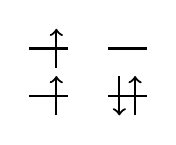
\begin{tikzpicture}
    % oberste MOs:
    \draw[thick] (0,0) -- (0.5,0); % erster Strich
    \draw[thick] (1,0) -- (1.5,0); % zweiter Strich
    % unterste MOs:
    \draw[thick] (0,-0.6) -- (0.5,-0.6); % dritter Strich
    \draw[thick] (1,-0.6) -- (1.5,-0.6); % vierter Strich
\draw[->, thick] (0.35, -0.25) -- (0.35, 0.25); 
\draw[-> , thick] (0.35, -0.85) -- (0.35, -0.35); 
 \draw[-> , thick] (1.35, -0.85) -- (1.35, -0.35); 
\draw[<- , thick] (1.15, -0.85) -- (1.15, -0.35); 
\end{tikzpicture} \qquad 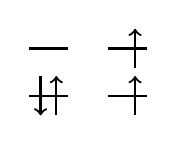
\begin{tikzpicture}
    % oberste MOs:
    \draw[thick] (0,0) -- (0.5,0); % erster Strich
    \draw[thick] (1,0) -- (1.5,0); % zweiter Strich
    % unterste MOs:
    \draw[thick] (0,-0.6) -- (0.5,-0.6); % dritter Strich
    \draw[thick] (1,-0.6) -- (1.5,-0.6); % vierter Strich
\draw[->, thick] (1.35, -0.25) -- (1.35, 0.25); 
\draw[-> , thick] (0.35, -0.85) -- (0.35, -0.35); 
\draw[<- , thick] (0.15, -0.85) -- (0.15, -0.35); 
 \draw[-> , thick] (1.35, -0.85) -- (1.35, -0.35); 
\end{tikzpicture}\right)\]$$+\cdot \underbrace{(b_{1u}^{l})\cdot (b_{2g}^{l})}_{\text{l: }b_{3u}}\cdot \underbrace{(a_{u}^{r})\cdot (b_{3g}^{r})}_{\text{r: }b_{3u}}\Rightarrow +\left|(b_{1u}^{l}) \cdot (b_{2g}^{l}) \cdot (b_{3g}^{r}) \cdot (a_{u}^{r})\right|$$$$=+\left|(+a_{g}+b_{1u}) \cdot (+b_{3u}+b_{2g}) \cdot (-b_{2u}+b_{3g}) \cdot (-b_{1g}+a_{u})\right|$$\begin{multline*}
=+\left|\underbrace{\overbrace{a_{g} b_{3u} b_{2u} b_{1g}}^{1 2 3 4}}_{a_{g}}\right|-\left|\underbrace{\overbrace{a_{g} b_{3u} b_{2u} a_{u}}^{1 2 3 8}}_{b_{1u}}\right|-\left|\underbrace{\overbrace{a_{g} b_{3u} b_{3g} b_{1g}}^{1 2 7 4}}_{b_{1u}}\right|+\left|\underbrace{\overbrace{a_{g} b_{3u} b_{3g} a_{u}}^{1 2 7 8}}_{a_{g}}\right|\\
+\left|\underbrace{\overbrace{a_{g} b_{2g} b_{2u} b_{1g}}^{1 6 3 4}}_{b_{1u}}\right|-\left|\underbrace{\overbrace{a_{g} b_{2g} b_{2u} a_{u}}^{1 6 3 8}}_{a_{g}}\right|-\left|\underbrace{\overbrace{a_{g} b_{2g} b_{3g} b_{1g}}^{1 6 7 4}}_{a_{g}}\right|+\left|\underbrace{\overbrace{a_{g} b_{2g} b_{3g} a_{u}}^{1 6 7 8}}_{b_{1u}}\right|\\
+\left|\underbrace{\overbrace{b_{1u} b_{3u} b_{2u} b_{1g}}^{5 2 3 4}}_{b_{1u}}\right|-\left|\underbrace{\overbrace{b_{1u} b_{3u} b_{2u} a_{u}}^{5 2 3 8}}_{a_{g}}\right|-\left|\underbrace{\overbrace{b_{1u} b_{3u} b_{3g} b_{1g}}^{5 2 7 4}}_{a_{g}}\right|+\left|\underbrace{\overbrace{b_{1u} b_{3u} b_{3g} a_{u}}^{5 2 7 8}}_{b_{1u}}\right|\\
+\left|\underbrace{\overbrace{b_{1u} b_{2g} b_{2u} b_{1g}}^{5 6 3 4}}_{a_{g}}\right|-\left|\underbrace{\overbrace{b_{1u} b_{2g} b_{2u} a_{u}}^{5 6 3 8}}_{b_{1u}}\right|-\left|\underbrace{\overbrace{b_{1u} b_{2g} b_{3g} b_{1g}}^{5 6 7 4}}_{b_{1u}}\right|+\left|\underbrace{\overbrace{b_{1u} b_{2g} b_{3g} a_{u}}^{5 6 7 8}}_{a_{g}}\right|
\end{multline*}\begin{multline*}
=+\left|\underbrace{\overbrace{a_{g} b_{3u} b_{2u} b_{1g}}^{1 2 3 4}}_{a_{g}}\right|-\left|\underbrace{\overbrace{a_{g} b_{3u} b_{2u} a_{u}}^{1 2 3 8}}_{b_{1u}}\right|+\left|\underbrace{\overbrace{a_{g} b_{3u} b_{1g} b_{3g}}^{1 2 4 7}}_{b_{1u}}\right|+\left|\underbrace{\overbrace{a_{g} b_{3u} b_{3g} a_{u}}^{1 2 7 8}}_{a_{g}}\right|\\
+\left|\underbrace{\overbrace{a_{g} b_{2u} b_{1g} b_{2g}}^{1 3 4 6}}_{b_{1u}}\right|+\left|\underbrace{\overbrace{a_{g} b_{2u} b_{2g} a_{u}}^{1 3 6 8}}_{a_{g}}\right|-\left|\underbrace{\overbrace{a_{g} b_{1g} b_{2g} b_{3g}}^{1 4 6 7}}_{a_{g}}\right|+\left|\underbrace{\overbrace{a_{g} b_{2g} b_{3g} a_{u}}^{1 6 7 8}}_{b_{1u}}\right|\\
-\left|\underbrace{\overbrace{b_{3u} b_{2u} b_{1g} b_{1u}}^{2 3 4 5}}_{b_{1u}}\right|-\left|\underbrace{\overbrace{b_{3u} b_{2u} b_{1u} a_{u}}^{2 3 5 8}}_{a_{g}}\right|+\left|\underbrace{\overbrace{b_{3u} b_{1g} b_{1u} b_{3g}}^{2 4 5 7}}_{a_{g}}\right|-\left|\underbrace{\overbrace{b_{3u} b_{1u} b_{3g} a_{u}}^{2 5 7 8}}_{b_{1u}}\right|\\
+\left|\underbrace{\overbrace{b_{2u} b_{1g} b_{1u} b_{2g}}^{3 4 5 6}}_{a_{g}}\right|-\left|\underbrace{\overbrace{b_{2u} b_{1u} b_{2g} a_{u}}^{3 5 6 8}}_{b_{1u}}\right|+\left|\underbrace{\overbrace{b_{1g} b_{1u} b_{2g} b_{3g}}^{4 5 6 7}}_{b_{1u}}\right|+\left|\underbrace{\overbrace{b_{1u} b_{2g} b_{3g} a_{u}}^{5 6 7 8}}_{a_{g}}\right|
\end{multline*}(nicht kürzbar)\\ \\
\vspace{0.5cm}

\[+\left(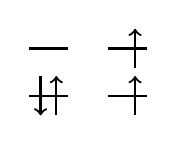
\begin{tikzpicture}
    % oberste MOs:
    \draw[thick] (0,0) -- (0.5,0); % erster Strich
    \draw[thick] (1,0) -- (1.5,0); % zweiter Strich
    % unterste MOs:
    \draw[thick] (0,-0.6) -- (0.5,-0.6); % dritter Strich
    \draw[thick] (1,-0.6) -- (1.5,-0.6); % vierter Strich
\draw[->, thick] (1.35, -0.25) -- (1.35, 0.25); 
\draw[-> , thick] (0.35, -0.85) -- (0.35, -0.35); 
\draw[<- , thick] (0.15, -0.85) -- (0.15, -0.35); 
 \draw[-> , thick] (1.35, -0.85) -- (1.35, -0.35); 
\end{tikzpicture} \qquad 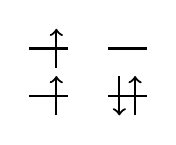
\begin{tikzpicture}
    % oberste MOs:
    \draw[thick] (0,0) -- (0.5,0); % erster Strich
    \draw[thick] (1,0) -- (1.5,0); % zweiter Strich
    % unterste MOs:
    \draw[thick] (0,-0.6) -- (0.5,-0.6); % dritter Strich
    \draw[thick] (1,-0.6) -- (1.5,-0.6); % vierter Strich
\draw[->, thick] (0.35, -0.25) -- (0.35, 0.25); 
\draw[-> , thick] (0.35, -0.85) -- (0.35, -0.35); 
 \draw[-> , thick] (1.35, -0.85) -- (1.35, -0.35); 
\draw[<- , thick] (1.15, -0.85) -- (1.15, -0.35); 
\end{tikzpicture}\right)\]$$+\cdot \underbrace{(a_{u}^{l})\cdot (b_{3g}^{l})}_{\text{l: }b_{3u}}\cdot \underbrace{(b_{1u}^{r})\cdot (b_{2g}^{r})}_{\text{r: }b_{3u}}\Rightarrow +\left|(b_{1u}^{r}) \cdot (b_{2g}^{r}) \cdot (b_{3g}^{l}) \cdot (a_{u}^{l})\right|$$$$=+\left|(-a_{g}+b_{1u}) \cdot (-b_{3u}+b_{2g}) \cdot (+b_{2u}+b_{3g}) \cdot (+b_{1g}+a_{u})\right|$$\begin{multline*}
=+\left|\underbrace{\overbrace{a_{g} b_{3u} b_{2u} b_{1g}}^{1 2 3 4}}_{a_{g}}\right|+\left|\underbrace{\overbrace{a_{g} b_{3u} b_{2u} a_{u}}^{1 2 3 8}}_{b_{1u}}\right|+\left|\underbrace{\overbrace{a_{g} b_{3u} b_{3g} b_{1g}}^{1 2 7 4}}_{b_{1u}}\right|+\left|\underbrace{\overbrace{a_{g} b_{3u} b_{3g} a_{u}}^{1 2 7 8}}_{a_{g}}\right|\\
-\left|\underbrace{\overbrace{a_{g} b_{2g} b_{2u} b_{1g}}^{1 6 3 4}}_{b_{1u}}\right|-\left|\underbrace{\overbrace{a_{g} b_{2g} b_{2u} a_{u}}^{1 6 3 8}}_{a_{g}}\right|-\left|\underbrace{\overbrace{a_{g} b_{2g} b_{3g} b_{1g}}^{1 6 7 4}}_{a_{g}}\right|-\left|\underbrace{\overbrace{a_{g} b_{2g} b_{3g} a_{u}}^{1 6 7 8}}_{b_{1u}}\right|\\
-\left|\underbrace{\overbrace{b_{1u} b_{3u} b_{2u} b_{1g}}^{5 2 3 4}}_{b_{1u}}\right|-\left|\underbrace{\overbrace{b_{1u} b_{3u} b_{2u} a_{u}}^{5 2 3 8}}_{a_{g}}\right|-\left|\underbrace{\overbrace{b_{1u} b_{3u} b_{3g} b_{1g}}^{5 2 7 4}}_{a_{g}}\right|-\left|\underbrace{\overbrace{b_{1u} b_{3u} b_{3g} a_{u}}^{5 2 7 8}}_{b_{1u}}\right|\\
+\left|\underbrace{\overbrace{b_{1u} b_{2g} b_{2u} b_{1g}}^{5 6 3 4}}_{a_{g}}\right|+\left|\underbrace{\overbrace{b_{1u} b_{2g} b_{2u} a_{u}}^{5 6 3 8}}_{b_{1u}}\right|+\left|\underbrace{\overbrace{b_{1u} b_{2g} b_{3g} b_{1g}}^{5 6 7 4}}_{b_{1u}}\right|+\left|\underbrace{\overbrace{b_{1u} b_{2g} b_{3g} a_{u}}^{5 6 7 8}}_{a_{g}}\right|
\end{multline*}\begin{multline*}
=+\left|\underbrace{\overbrace{a_{g} b_{3u} b_{2u} b_{1g}}^{1 2 3 4}}_{a_{g}}\right|+\left|\underbrace{\overbrace{a_{g} b_{3u} b_{2u} a_{u}}^{1 2 3 8}}_{b_{1u}}\right|-\left|\underbrace{\overbrace{a_{g} b_{3u} b_{1g} b_{3g}}^{1 2 4 7}}_{b_{1u}}\right|+\left|\underbrace{\overbrace{a_{g} b_{3u} b_{3g} a_{u}}^{1 2 7 8}}_{a_{g}}\right|\\
-\left|\underbrace{\overbrace{a_{g} b_{2u} b_{1g} b_{2g}}^{1 3 4 6}}_{b_{1u}}\right|+\left|\underbrace{\overbrace{a_{g} b_{2u} b_{2g} a_{u}}^{1 3 6 8}}_{a_{g}}\right|-\left|\underbrace{\overbrace{a_{g} b_{1g} b_{2g} b_{3g}}^{1 4 6 7}}_{a_{g}}\right|-\left|\underbrace{\overbrace{a_{g} b_{2g} b_{3g} a_{u}}^{1 6 7 8}}_{b_{1u}}\right|\\
+\left|\underbrace{\overbrace{b_{3u} b_{2u} b_{1g} b_{1u}}^{2 3 4 5}}_{b_{1u}}\right|-\left|\underbrace{\overbrace{b_{3u} b_{2u} b_{1u} a_{u}}^{2 3 5 8}}_{a_{g}}\right|+\left|\underbrace{\overbrace{b_{3u} b_{1g} b_{1u} b_{3g}}^{2 4 5 7}}_{a_{g}}\right|+\left|\underbrace{\overbrace{b_{3u} b_{1u} b_{3g} a_{u}}^{2 5 7 8}}_{b_{1u}}\right|\\
+\left|\underbrace{\overbrace{b_{2u} b_{1g} b_{1u} b_{2g}}^{3 4 5 6}}_{a_{g}}\right|+\left|\underbrace{\overbrace{b_{2u} b_{1u} b_{2g} a_{u}}^{3 5 6 8}}_{b_{1u}}\right|-\left|\underbrace{\overbrace{b_{1g} b_{1u} b_{2g} b_{3g}}^{4 5 6 7}}_{b_{1u}}\right|+\left|\underbrace{\overbrace{b_{1u} b_{2g} b_{3g} a_{u}}^{5 6 7 8}}_{a_{g}}\right|
\end{multline*}(nicht kürzbar)\\ \\
\hrule\newpage 


\[+\left(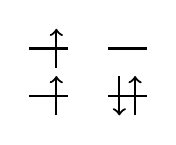
\begin{tikzpicture}
    % oberste MOs:
    \draw[thick] (0,0) -- (0.5,0); % erster Strich
    \draw[thick] (1,0) -- (1.5,0); % zweiter Strich
    % unterste MOs:
    \draw[thick] (0,-0.6) -- (0.5,-0.6); % dritter Strich
    \draw[thick] (1,-0.6) -- (1.5,-0.6); % vierter Strich
\draw[->, thick] (0.35, -0.25) -- (0.35, 0.25); 
\draw[-> , thick] (0.35, -0.85) -- (0.35, -0.35); 
 \draw[-> , thick] (1.35, -0.85) -- (1.35, -0.35); 
\draw[<- , thick] (1.15, -0.85) -- (1.15, -0.35); 
\end{tikzpicture} \qquad 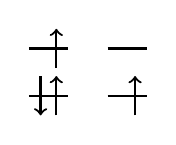
\begin{tikzpicture}
    % oberste MOs:
    \draw[thick] (0,0) -- (0.5,0); % erster Strich
    \draw[thick] (1,0) -- (1.5,0); % zweiter Strich
    % unterste MOs:
    \draw[thick] (0,-0.6) -- (0.5,-0.6); % dritter Strich
    \draw[thick] (1,-0.6) -- (1.5,-0.6); % vierter Strich
\draw[->, thick] (0.35, -0.25) -- (0.35, 0.25); 
\draw[-> , thick] (0.35, -0.85) -- (0.35, -0.35); 
\draw[<- , thick] (0.15, -0.85) -- (0.15, -0.35); 
 \draw[-> , thick] (1.35, -0.85) -- (1.35, -0.35); 
\end{tikzpicture}\right)\]$$+\cdot \underbrace{(b_{1u}^{l})\cdot (b_{2g}^{l})}_{\text{l: }b_{3u}}\cdot \underbrace{(b_{1u}^{r})\cdot (b_{3g}^{r})}_{\text{r: }b_{2u}}\Rightarrow +\left|(b_{1u}^{l}) \cdot (b_{1u}^{r}) \cdot (b_{2g}^{l}) \cdot (b_{3g}^{r})\right|$$$$=+\left|(+a_{g}+b_{1u}) \cdot (-a_{g}+b_{1u}) \cdot (+b_{3u}+b_{2g}) \cdot (-b_{2u}+b_{3g})\right|$$\begin{multline*}
=-\left|\underbrace{\overbrace{a_{g} b_{1u} b_{3u} b_{2u}}^{1 5 2 3}}_{a_{u}}\right|+\left|\underbrace{\overbrace{a_{g} b_{1u} b_{3u} b_{3g}}^{1 5 2 7}}_{b_{1g}}\right|-\left|\underbrace{\overbrace{a_{g} b_{1u} b_{2g} b_{2u}}^{1 5 6 3}}_{b_{1g}}\right|+\left|\underbrace{\overbrace{a_{g} b_{1u} b_{2g} b_{3g}}^{1 5 6 7}}_{a_{u}}\right|\\
+\left|\underbrace{\overbrace{b_{1u} a_{g} b_{3u} b_{2u}}^{5 1 2 3}}_{a_{u}}\right|-\left|\underbrace{\overbrace{b_{1u} a_{g} b_{3u} b_{3g}}^{5 1 2 7}}_{b_{1g}}\right|+\left|\underbrace{\overbrace{b_{1u} a_{g} b_{2g} b_{2u}}^{5 1 6 3}}_{b_{1g}}\right|-\left|\underbrace{\overbrace{b_{1u} a_{g} b_{2g} b_{3g}}^{5 1 6 7}}_{a_{u}}\right|\\
\end{multline*}\begin{multline*}
=-\left|\underbrace{\overbrace{a_{g} b_{3u} b_{2u} b_{1u}}^{1 2 3 5}}_{a_{u}}\right|-\left|\underbrace{\overbrace{a_{g} b_{3u} b_{1u} b_{3g}}^{1 2 5 7}}_{b_{1g}}\right|-\left|\underbrace{\overbrace{a_{g} b_{2u} b_{1u} b_{2g}}^{1 3 5 6}}_{b_{1g}}\right|+\left|\underbrace{\overbrace{a_{g} b_{1u} b_{2g} b_{3g}}^{1 5 6 7}}_{a_{u}}\right|\\
-\left|\underbrace{\overbrace{a_{g} b_{3u} b_{2u} b_{1u}}^{1 2 3 5}}_{a_{u}}\right|-\left|\underbrace{\overbrace{a_{g} b_{3u} b_{1u} b_{3g}}^{1 2 5 7}}_{b_{1g}}\right|-\left|\underbrace{\overbrace{a_{g} b_{2u} b_{1u} b_{2g}}^{1 3 5 6}}_{b_{1g}}\right|+\left|\underbrace{\overbrace{a_{g} b_{1u} b_{2g} b_{3g}}^{1 5 6 7}}_{a_{u}}\right|\\
\end{multline*}zusammengefasst:\begin{multline*}
=-2\left|\underbrace{\overbrace{a_{g} b_{3u} b_{2u} b_{1u}}^{1 2 3 5}}_{a_{u}}\right|-2\left|\underbrace{\overbrace{a_{g} b_{3u} b_{1u} b_{3g}}^{1 2 5 7}}_{b_{1g}}\right|-2\left|\underbrace{\overbrace{a_{g} b_{2u} b_{1u} b_{2g}}^{1 3 5 6}}_{b_{1g}}\right|+2\left|\underbrace{\overbrace{a_{g} b_{1u} b_{2g} b_{3g}}^{1 5 6 7}}_{a_{u}}\right|\\
\end{multline*}\\ \\
\vspace{0.5cm}

\[+\left(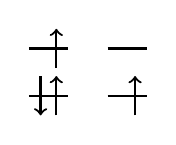
\begin{tikzpicture}
    % oberste MOs:
    \draw[thick] (0,0) -- (0.5,0); % erster Strich
    \draw[thick] (1,0) -- (1.5,0); % zweiter Strich
    % unterste MOs:
    \draw[thick] (0,-0.6) -- (0.5,-0.6); % dritter Strich
    \draw[thick] (1,-0.6) -- (1.5,-0.6); % vierter Strich
\draw[->, thick] (0.35, -0.25) -- (0.35, 0.25); 
\draw[-> , thick] (0.35, -0.85) -- (0.35, -0.35); 
\draw[<- , thick] (0.15, -0.85) -- (0.15, -0.35); 
 \draw[-> , thick] (1.35, -0.85) -- (1.35, -0.35); 
\end{tikzpicture} \qquad 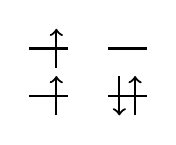
\begin{tikzpicture}
    % oberste MOs:
    \draw[thick] (0,0) -- (0.5,0); % erster Strich
    \draw[thick] (1,0) -- (1.5,0); % zweiter Strich
    % unterste MOs:
    \draw[thick] (0,-0.6) -- (0.5,-0.6); % dritter Strich
    \draw[thick] (1,-0.6) -- (1.5,-0.6); % vierter Strich
\draw[->, thick] (0.35, -0.25) -- (0.35, 0.25); 
\draw[-> , thick] (0.35, -0.85) -- (0.35, -0.35); 
 \draw[-> , thick] (1.35, -0.85) -- (1.35, -0.35); 
\draw[<- , thick] (1.15, -0.85) -- (1.15, -0.35); 
\end{tikzpicture}\right)\]$$+\cdot \underbrace{(b_{1u}^{l})\cdot (b_{3g}^{l})}_{\text{l: }b_{2u}}\cdot \underbrace{(b_{1u}^{r})\cdot (b_{2g}^{r})}_{\text{r: }b_{3u}}\Rightarrow +\left|(b_{1u}^{l}) \cdot (b_{1u}^{r}) \cdot (b_{2g}^{r}) \cdot (b_{3g}^{l})\right|$$$$=+\left|(+a_{g}+b_{1u}) \cdot (-a_{g}+b_{1u}) \cdot (-b_{3u}+b_{2g}) \cdot (+b_{2u}+b_{3g})\right|$$\begin{multline*}
=-\left|\underbrace{\overbrace{a_{g} b_{1u} b_{3u} b_{2u}}^{1 5 2 3}}_{a_{u}}\right|-\left|\underbrace{\overbrace{a_{g} b_{1u} b_{3u} b_{3g}}^{1 5 2 7}}_{b_{1g}}\right|+\left|\underbrace{\overbrace{a_{g} b_{1u} b_{2g} b_{2u}}^{1 5 6 3}}_{b_{1g}}\right|+\left|\underbrace{\overbrace{a_{g} b_{1u} b_{2g} b_{3g}}^{1 5 6 7}}_{a_{u}}\right|\\
+\left|\underbrace{\overbrace{b_{1u} a_{g} b_{3u} b_{2u}}^{5 1 2 3}}_{a_{u}}\right|+\left|\underbrace{\overbrace{b_{1u} a_{g} b_{3u} b_{3g}}^{5 1 2 7}}_{b_{1g}}\right|-\left|\underbrace{\overbrace{b_{1u} a_{g} b_{2g} b_{2u}}^{5 1 6 3}}_{b_{1g}}\right|-\left|\underbrace{\overbrace{b_{1u} a_{g} b_{2g} b_{3g}}^{5 1 6 7}}_{a_{u}}\right|\\
\end{multline*}\begin{multline*}
=-\left|\underbrace{\overbrace{a_{g} b_{3u} b_{2u} b_{1u}}^{1 2 3 5}}_{a_{u}}\right|+\left|\underbrace{\overbrace{a_{g} b_{3u} b_{1u} b_{3g}}^{1 2 5 7}}_{b_{1g}}\right|+\left|\underbrace{\overbrace{a_{g} b_{2u} b_{1u} b_{2g}}^{1 3 5 6}}_{b_{1g}}\right|+\left|\underbrace{\overbrace{a_{g} b_{1u} b_{2g} b_{3g}}^{1 5 6 7}}_{a_{u}}\right|\\
-\left|\underbrace{\overbrace{a_{g} b_{3u} b_{2u} b_{1u}}^{1 2 3 5}}_{a_{u}}\right|+\left|\underbrace{\overbrace{a_{g} b_{3u} b_{1u} b_{3g}}^{1 2 5 7}}_{b_{1g}}\right|+\left|\underbrace{\overbrace{a_{g} b_{2u} b_{1u} b_{2g}}^{1 3 5 6}}_{b_{1g}}\right|+\left|\underbrace{\overbrace{a_{g} b_{1u} b_{2g} b_{3g}}^{1 5 6 7}}_{a_{u}}\right|\\
\end{multline*}zusammengefasst:\begin{multline*}
=-2\left|\underbrace{\overbrace{a_{g} b_{3u} b_{2u} b_{1u}}^{1 2 3 5}}_{a_{u}}\right|+2\left|\underbrace{\overbrace{a_{g} b_{3u} b_{1u} b_{3g}}^{1 2 5 7}}_{b_{1g}}\right|+2\left|\underbrace{\overbrace{a_{g} b_{2u} b_{1u} b_{2g}}^{1 3 5 6}}_{b_{1g}}\right|+2\left|\underbrace{\overbrace{a_{g} b_{1u} b_{2g} b_{3g}}^{1 5 6 7}}_{a_{u}}\right|\\
\end{multline*}\\ \\
\hrule\newpage 


\[+\left(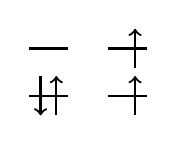
\begin{tikzpicture}
    % oberste MOs:
    \draw[thick] (0,0) -- (0.5,0); % erster Strich
    \draw[thick] (1,0) -- (1.5,0); % zweiter Strich
    % unterste MOs:
    \draw[thick] (0,-0.6) -- (0.5,-0.6); % dritter Strich
    \draw[thick] (1,-0.6) -- (1.5,-0.6); % vierter Strich
\draw[->, thick] (1.35, -0.25) -- (1.35, 0.25); 
\draw[-> , thick] (0.35, -0.85) -- (0.35, -0.35); 
\draw[<- , thick] (0.15, -0.85) -- (0.15, -0.35); 
 \draw[-> , thick] (1.35, -0.85) -- (1.35, -0.35); 
\end{tikzpicture} \qquad 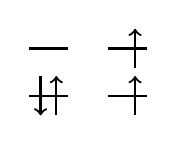
\begin{tikzpicture}
    % oberste MOs:
    \draw[thick] (0,0) -- (0.5,0); % erster Strich
    \draw[thick] (1,0) -- (1.5,0); % zweiter Strich
    % unterste MOs:
    \draw[thick] (0,-0.6) -- (0.5,-0.6); % dritter Strich
    \draw[thick] (1,-0.6) -- (1.5,-0.6); % vierter Strich
\draw[->, thick] (1.35, -0.25) -- (1.35, 0.25); 
\draw[-> , thick] (0.35, -0.85) -- (0.35, -0.35); 
\draw[<- , thick] (0.15, -0.85) -- (0.15, -0.35); 
 \draw[-> , thick] (1.35, -0.85) -- (1.35, -0.35); 
\end{tikzpicture}\right)\]$$+\cdot \underbrace{(a_{u}^{l})\cdot (b_{3g}^{l})}_{\text{l: }b_{3u}}\cdot \underbrace{(a_{u}^{r})\cdot (b_{3g}^{r})}_{\text{r: }b_{3u}}\Rightarrow +\left|(b_{3g}^{l}) \cdot (b_{3g}^{r}) \cdot (a_{u}^{l}) \cdot (a_{u}^{r})\right|$$$$=+\left|(+b_{2u}+b_{3g}) \cdot (-b_{2u}+b_{3g}) \cdot (+b_{1g}+a_{u}) \cdot (-b_{1g}+a_{u})\right|$$\begin{multline*}
=+\left|\underbrace{\overbrace{b_{2u} b_{3g} b_{1g} a_{u}}^{3 7 4 8}}_{a_{g}}\right|-\left|\underbrace{\overbrace{b_{2u} b_{3g} a_{u} b_{1g}}^{3 7 8 4}}_{a_{g}}\right|-\left|\underbrace{\overbrace{b_{3g} b_{2u} b_{1g} a_{u}}^{7 3 4 8}}_{a_{g}}\right|+\left|\underbrace{\overbrace{b_{3g} b_{2u} a_{u} b_{1g}}^{7 3 8 4}}_{a_{g}}\right|\\
\end{multline*}\begin{multline*}
=-\left|\underbrace{\overbrace{b_{2u} b_{1g} b_{3g} a_{u}}^{3 4 7 8}}_{a_{g}}\right|-\left|\underbrace{\overbrace{b_{2u} b_{1g} b_{3g} a_{u}}^{3 4 7 8}}_{a_{g}}\right|-\left|\underbrace{\overbrace{b_{2u} b_{1g} b_{3g} a_{u}}^{3 4 7 8}}_{a_{g}}\right|-\left|\underbrace{\overbrace{b_{2u} b_{1g} b_{3g} a_{u}}^{3 4 7 8}}_{a_{g}}\right|\\
\end{multline*}zusammengefasst:\begin{multline*}
=-4\left|\underbrace{\overbrace{b_{2u} b_{1g} b_{3g} a_{u}}^{3 4 7 8}}_{a_{g}}\right|
\end{multline*}\\ \\
\hrule\newpage 


\[+\left(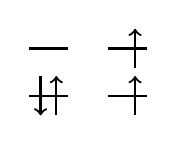
\begin{tikzpicture}
    % oberste MOs:
    \draw[thick] (0,0) -- (0.5,0); % erster Strich
    \draw[thick] (1,0) -- (1.5,0); % zweiter Strich
    % unterste MOs:
    \draw[thick] (0,-0.6) -- (0.5,-0.6); % dritter Strich
    \draw[thick] (1,-0.6) -- (1.5,-0.6); % vierter Strich
\draw[->, thick] (1.35, -0.25) -- (1.35, 0.25); 
\draw[-> , thick] (0.35, -0.85) -- (0.35, -0.35); 
\draw[<- , thick] (0.15, -0.85) -- (0.15, -0.35); 
 \draw[-> , thick] (1.35, -0.85) -- (1.35, -0.35); 
\end{tikzpicture} \qquad 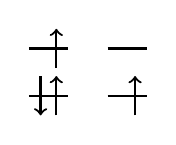
\begin{tikzpicture}
    % oberste MOs:
    \draw[thick] (0,0) -- (0.5,0); % erster Strich
    \draw[thick] (1,0) -- (1.5,0); % zweiter Strich
    % unterste MOs:
    \draw[thick] (0,-0.6) -- (0.5,-0.6); % dritter Strich
    \draw[thick] (1,-0.6) -- (1.5,-0.6); % vierter Strich
\draw[->, thick] (0.35, -0.25) -- (0.35, 0.25); 
\draw[-> , thick] (0.35, -0.85) -- (0.35, -0.35); 
\draw[<- , thick] (0.15, -0.85) -- (0.15, -0.35); 
 \draw[-> , thick] (1.35, -0.85) -- (1.35, -0.35); 
\end{tikzpicture}\right)\]$$+\cdot \underbrace{(a_{u}^{l})\cdot (b_{3g}^{l})}_{\text{l: }b_{3u}}\cdot \underbrace{(b_{1u}^{r})\cdot (b_{3g}^{r})}_{\text{r: }b_{2u}}\Rightarrow +\left|(b_{1u}^{r}) \cdot (b_{3g}^{l}) \cdot (b_{3g}^{r}) \cdot (a_{u}^{l})\right|$$$$=+\left|(-a_{g}+b_{1u}) \cdot (+b_{2u}+b_{3g}) \cdot (-b_{2u}+b_{3g}) \cdot (+b_{1g}+a_{u})\right|$$\begin{multline*}
=-\left|\underbrace{\overbrace{a_{g} b_{2u} b_{3g} b_{1g}}^{1 3 7 4}}_{a_{u}}\right|-\left|\underbrace{\overbrace{a_{g} b_{2u} b_{3g} a_{u}}^{1 3 7 8}}_{b_{1g}}\right|+\left|\underbrace{\overbrace{a_{g} b_{3g} b_{2u} b_{1g}}^{1 7 3 4}}_{a_{u}}\right|+\left|\underbrace{\overbrace{a_{g} b_{3g} b_{2u} a_{u}}^{1 7 3 8}}_{b_{1g}}\right|\\
+\left|\underbrace{\overbrace{b_{1u} b_{2u} b_{3g} b_{1g}}^{5 3 7 4}}_{b_{1g}}\right|+\left|\underbrace{\overbrace{b_{1u} b_{2u} b_{3g} a_{u}}^{5 3 7 8}}_{a_{u}}\right|-\left|\underbrace{\overbrace{b_{1u} b_{3g} b_{2u} b_{1g}}^{5 7 3 4}}_{b_{1g}}\right|-\left|\underbrace{\overbrace{b_{1u} b_{3g} b_{2u} a_{u}}^{5 7 3 8}}_{a_{u}}\right|\\
\end{multline*}\begin{multline*}
=+\left|\underbrace{\overbrace{a_{g} b_{2u} b_{1g} b_{3g}}^{1 3 4 7}}_{a_{u}}\right|-\left|\underbrace{\overbrace{a_{g} b_{2u} b_{3g} a_{u}}^{1 3 7 8}}_{b_{1g}}\right|+\left|\underbrace{\overbrace{a_{g} b_{2u} b_{1g} b_{3g}}^{1 3 4 7}}_{a_{u}}\right|-\left|\underbrace{\overbrace{a_{g} b_{2u} b_{3g} a_{u}}^{1 3 7 8}}_{b_{1g}}\right|\\
-\left|\underbrace{\overbrace{b_{2u} b_{1g} b_{1u} b_{3g}}^{3 4 5 7}}_{b_{1g}}\right|-\left|\underbrace{\overbrace{b_{2u} b_{1u} b_{3g} a_{u}}^{3 5 7 8}}_{a_{u}}\right|-\left|\underbrace{\overbrace{b_{2u} b_{1g} b_{1u} b_{3g}}^{3 4 5 7}}_{b_{1g}}\right|-\left|\underbrace{\overbrace{b_{2u} b_{1u} b_{3g} a_{u}}^{3 5 7 8}}_{a_{u}}\right|\\
\end{multline*}zusammengefasst:\begin{multline*}
=+2\left|\underbrace{\overbrace{a_{g} b_{2u} b_{1g} b_{3g}}^{1 3 4 7}}_{a_{u}}\right|-2\left|\underbrace{\overbrace{a_{g} b_{2u} b_{3g} a_{u}}^{1 3 7 8}}_{b_{1g}}\right|-2\left|\underbrace{\overbrace{b_{2u} b_{1g} b_{1u} b_{3g}}^{3 4 5 7}}_{b_{1g}}\right|-2\left|\underbrace{\overbrace{b_{2u} b_{1u} b_{3g} a_{u}}^{3 5 7 8}}_{a_{u}}\right|\\
\end{multline*}\\ \\
\vspace{0.5cm}

\[+\left(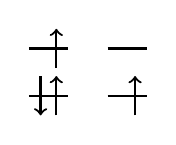
\begin{tikzpicture}
    % oberste MOs:
    \draw[thick] (0,0) -- (0.5,0); % erster Strich
    \draw[thick] (1,0) -- (1.5,0); % zweiter Strich
    % unterste MOs:
    \draw[thick] (0,-0.6) -- (0.5,-0.6); % dritter Strich
    \draw[thick] (1,-0.6) -- (1.5,-0.6); % vierter Strich
\draw[->, thick] (0.35, -0.25) -- (0.35, 0.25); 
\draw[-> , thick] (0.35, -0.85) -- (0.35, -0.35); 
\draw[<- , thick] (0.15, -0.85) -- (0.15, -0.35); 
 \draw[-> , thick] (1.35, -0.85) -- (1.35, -0.35); 
\end{tikzpicture} \qquad 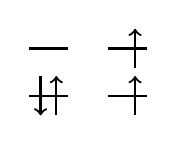
\begin{tikzpicture}
    % oberste MOs:
    \draw[thick] (0,0) -- (0.5,0); % erster Strich
    \draw[thick] (1,0) -- (1.5,0); % zweiter Strich
    % unterste MOs:
    \draw[thick] (0,-0.6) -- (0.5,-0.6); % dritter Strich
    \draw[thick] (1,-0.6) -- (1.5,-0.6); % vierter Strich
\draw[->, thick] (1.35, -0.25) -- (1.35, 0.25); 
\draw[-> , thick] (0.35, -0.85) -- (0.35, -0.35); 
\draw[<- , thick] (0.15, -0.85) -- (0.15, -0.35); 
 \draw[-> , thick] (1.35, -0.85) -- (1.35, -0.35); 
\end{tikzpicture}\right)\]$$+\cdot \underbrace{(b_{1u}^{l})\cdot (b_{3g}^{l})}_{\text{l: }b_{2u}}\cdot \underbrace{(a_{u}^{r})\cdot (b_{3g}^{r})}_{\text{r: }b_{3u}}\Rightarrow +\left|(b_{1u}^{l}) \cdot (b_{3g}^{l}) \cdot (b_{3g}^{r}) \cdot (a_{u}^{r})\right|$$$$=+\left|(+a_{g}+b_{1u}) \cdot (+b_{2u}+b_{3g}) \cdot (-b_{2u}+b_{3g}) \cdot (-b_{1g}+a_{u})\right|$$\begin{multline*}
=-\left|\underbrace{\overbrace{a_{g} b_{2u} b_{3g} b_{1g}}^{1 3 7 4}}_{a_{u}}\right|+\left|\underbrace{\overbrace{a_{g} b_{2u} b_{3g} a_{u}}^{1 3 7 8}}_{b_{1g}}\right|+\left|\underbrace{\overbrace{a_{g} b_{3g} b_{2u} b_{1g}}^{1 7 3 4}}_{a_{u}}\right|-\left|\underbrace{\overbrace{a_{g} b_{3g} b_{2u} a_{u}}^{1 7 3 8}}_{b_{1g}}\right|\\
-\left|\underbrace{\overbrace{b_{1u} b_{2u} b_{3g} b_{1g}}^{5 3 7 4}}_{b_{1g}}\right|+\left|\underbrace{\overbrace{b_{1u} b_{2u} b_{3g} a_{u}}^{5 3 7 8}}_{a_{u}}\right|+\left|\underbrace{\overbrace{b_{1u} b_{3g} b_{2u} b_{1g}}^{5 7 3 4}}_{b_{1g}}\right|-\left|\underbrace{\overbrace{b_{1u} b_{3g} b_{2u} a_{u}}^{5 7 3 8}}_{a_{u}}\right|\\
\end{multline*}\begin{multline*}
=+\left|\underbrace{\overbrace{a_{g} b_{2u} b_{1g} b_{3g}}^{1 3 4 7}}_{a_{u}}\right|+\left|\underbrace{\overbrace{a_{g} b_{2u} b_{3g} a_{u}}^{1 3 7 8}}_{b_{1g}}\right|+\left|\underbrace{\overbrace{a_{g} b_{2u} b_{1g} b_{3g}}^{1 3 4 7}}_{a_{u}}\right|+\left|\underbrace{\overbrace{a_{g} b_{2u} b_{3g} a_{u}}^{1 3 7 8}}_{b_{1g}}\right|\\
+\left|\underbrace{\overbrace{b_{2u} b_{1g} b_{1u} b_{3g}}^{3 4 5 7}}_{b_{1g}}\right|-\left|\underbrace{\overbrace{b_{2u} b_{1u} b_{3g} a_{u}}^{3 5 7 8}}_{a_{u}}\right|+\left|\underbrace{\overbrace{b_{2u} b_{1g} b_{1u} b_{3g}}^{3 4 5 7}}_{b_{1g}}\right|-\left|\underbrace{\overbrace{b_{2u} b_{1u} b_{3g} a_{u}}^{3 5 7 8}}_{a_{u}}\right|\\
\end{multline*}zusammengefasst:\begin{multline*}
=+2\left|\underbrace{\overbrace{a_{g} b_{2u} b_{1g} b_{3g}}^{1 3 4 7}}_{a_{u}}\right|+2\left|\underbrace{\overbrace{a_{g} b_{2u} b_{3g} a_{u}}^{1 3 7 8}}_{b_{1g}}\right|+2\left|\underbrace{\overbrace{b_{2u} b_{1g} b_{1u} b_{3g}}^{3 4 5 7}}_{b_{1g}}\right|-2\left|\underbrace{\overbrace{b_{2u} b_{1u} b_{3g} a_{u}}^{3 5 7 8}}_{a_{u}}\right|\\
\end{multline*}\\ \\
\hrule\newpage 


\[+\left(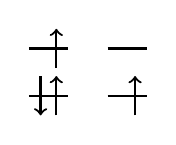
\begin{tikzpicture}
    % oberste MOs:
    \draw[thick] (0,0) -- (0.5,0); % erster Strich
    \draw[thick] (1,0) -- (1.5,0); % zweiter Strich
    % unterste MOs:
    \draw[thick] (0,-0.6) -- (0.5,-0.6); % dritter Strich
    \draw[thick] (1,-0.6) -- (1.5,-0.6); % vierter Strich
\draw[->, thick] (0.35, -0.25) -- (0.35, 0.25); 
\draw[-> , thick] (0.35, -0.85) -- (0.35, -0.35); 
\draw[<- , thick] (0.15, -0.85) -- (0.15, -0.35); 
 \draw[-> , thick] (1.35, -0.85) -- (1.35, -0.35); 
\end{tikzpicture} \qquad 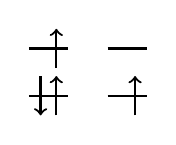
\begin{tikzpicture}
    % oberste MOs:
    \draw[thick] (0,0) -- (0.5,0); % erster Strich
    \draw[thick] (1,0) -- (1.5,0); % zweiter Strich
    % unterste MOs:
    \draw[thick] (0,-0.6) -- (0.5,-0.6); % dritter Strich
    \draw[thick] (1,-0.6) -- (1.5,-0.6); % vierter Strich
\draw[->, thick] (0.35, -0.25) -- (0.35, 0.25); 
\draw[-> , thick] (0.35, -0.85) -- (0.35, -0.35); 
\draw[<- , thick] (0.15, -0.85) -- (0.15, -0.35); 
 \draw[-> , thick] (1.35, -0.85) -- (1.35, -0.35); 
\end{tikzpicture}\right)\]$$+\cdot \underbrace{(b_{1u}^{l})\cdot (b_{3g}^{l})}_{\text{l: }b_{2u}}\cdot \underbrace{(b_{1u}^{r})\cdot (b_{3g}^{r})}_{\text{r: }b_{2u}}\Rightarrow +\left|(b_{1u}^{l}) \cdot (b_{1u}^{r}) \cdot (b_{3g}^{l}) \cdot (b_{3g}^{r})\right|$$$$=+\left|(+a_{g}+b_{1u}) \cdot (-a_{g}+b_{1u}) \cdot (+b_{2u}+b_{3g}) \cdot (-b_{2u}+b_{3g})\right|$$\begin{multline*}
=+\left|\underbrace{\overbrace{a_{g} b_{1u} b_{2u} b_{3g}}^{1 5 3 7}}_{a_{g}}\right|-\left|\underbrace{\overbrace{a_{g} b_{1u} b_{3g} b_{2u}}^{1 5 7 3}}_{a_{g}}\right|-\left|\underbrace{\overbrace{b_{1u} a_{g} b_{2u} b_{3g}}^{5 1 3 7}}_{a_{g}}\right|+\left|\underbrace{\overbrace{b_{1u} a_{g} b_{3g} b_{2u}}^{5 1 7 3}}_{a_{g}}\right|\\
\end{multline*}\begin{multline*}
=-\left|\underbrace{\overbrace{a_{g} b_{2u} b_{1u} b_{3g}}^{1 3 5 7}}_{a_{g}}\right|-\left|\underbrace{\overbrace{a_{g} b_{2u} b_{1u} b_{3g}}^{1 3 5 7}}_{a_{g}}\right|-\left|\underbrace{\overbrace{a_{g} b_{2u} b_{1u} b_{3g}}^{1 3 5 7}}_{a_{g}}\right|-\left|\underbrace{\overbrace{a_{g} b_{2u} b_{1u} b_{3g}}^{1 3 5 7}}_{a_{g}}\right|\\
\end{multline*}zusammengefasst:\begin{multline*}
=-4\left|\underbrace{\overbrace{a_{g} b_{2u} b_{1u} b_{3g}}^{1 3 5 7}}_{a_{g}}\right|
\end{multline*}\\ \\
\hrule\newpage 

\newpage \section{Linearkombinationen: 4 Monomer- / 2 Dimer-Zustände}
\[ +\left(\text{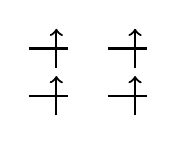
\begin{tikzpicture}
    % oberste MOs:
    \draw[thick] (0,0) -- (0.5,0); % erster Strich
    \draw[thick] (1,0) -- (1.5,0); % zweiter Strich
    % unterste MOs:
    \draw[thick] (0,-0.6) -- (0.5,-0.6); % dritter Strich
    \draw[thick] (1,-0.6) -- (1.5,-0.6); % vierter Strich
\draw[->, thick] (0.35, -0.25) -- (0.35, 0.25); 
\draw[->, thick] (1.35, -0.25) -- (1.35, 0.25); 
\draw[-> , thick] (0.35, -0.85) -- (0.35, -0.35); 
 \draw[-> , thick] (1.35, -0.85) -- (1.35, -0.35); 
\end{tikzpicture} \qquad 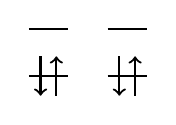
\begin{tikzpicture}
    % oberste MOs:
    \draw[thick] (0,0) -- (0.5,0); % erster Strich
    \draw[thick] (1,0) -- (1.5,0); % zweiter Strich
    % unterste MOs:
    \draw[thick] (0,-0.6) -- (0.5,-0.6); % dritter Strich
    \draw[thick] (1,-0.6) -- (1.5,-0.6); % vierter Strich
\draw[-> , thick] (0.35, -0.85) -- (0.35, -0.35); 
\draw[<- , thick] (0.15, -0.85) -- (0.15, -0.35); 
 \draw[-> , thick] (1.35, -0.85) -- (1.35, -0.35); 
\draw[<- , thick] (1.15, -0.85) -- (1.15, -0.35); 
\end{tikzpicture}}\right)+\left(\text{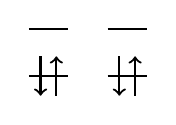
\begin{tikzpicture}
    % oberste MOs:
    \draw[thick] (0,0) -- (0.5,0); % erster Strich
    \draw[thick] (1,0) -- (1.5,0); % zweiter Strich
    % unterste MOs:
    \draw[thick] (0,-0.6) -- (0.5,-0.6); % dritter Strich
    \draw[thick] (1,-0.6) -- (1.5,-0.6); % vierter Strich
\draw[-> , thick] (0.35, -0.85) -- (0.35, -0.35); 
\draw[<- , thick] (0.15, -0.85) -- (0.15, -0.35); 
 \draw[-> , thick] (1.35, -0.85) -- (1.35, -0.35); 
\draw[<- , thick] (1.15, -0.85) -- (1.15, -0.35); 
\end{tikzpicture} \qquad 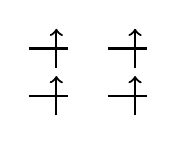
\begin{tikzpicture}
    % oberste MOs:
    \draw[thick] (0,0) -- (0.5,0); % erster Strich
    \draw[thick] (1,0) -- (1.5,0); % zweiter Strich
    % unterste MOs:
    \draw[thick] (0,-0.6) -- (0.5,-0.6); % dritter Strich
    \draw[thick] (1,-0.6) -- (1.5,-0.6); % vierter Strich
\draw[->, thick] (0.35, -0.25) -- (0.35, 0.25); 
\draw[->, thick] (1.35, -0.25) -- (1.35, 0.25); 
\draw[-> , thick] (0.35, -0.85) -- (0.35, -0.35); 
 \draw[-> , thick] (1.35, -0.85) -- (1.35, -0.35); 
\end{tikzpicture}}\right)\]enthaltene Monomer-Symmetrien = $a_{g}$\begin{multline*}=+\left(\left|(b_{1u}^{l}) \cdot (b_{2g}^{l}) \cdot (b_{3g}^{l}) \cdot (a_{u}^{l})\right|\right)+\left(\left|(b_{1u}^{r}) \cdot (b_{2g}^{r}) \cdot (b_{3g}^{r}) \cdot (a_{u}^{r})\right|\right)\end{multline*}
\begin{multline*}
=+2\left|\underbrace{\overbrace{a_{g} b_{3u} b_{2u} b_{1g}}^{1 2 3 4}}_{a_{g}}\right|+2\left|\underbrace{\overbrace{a_{g} b_{3u} b_{3g} a_{u}}^{1 2 7 8}}_{a_{g}}\right|-2\left|\underbrace{\overbrace{a_{g} b_{2u} b_{2g} a_{u}}^{1 3 6 8}}_{a_{g}}\right|+2\left|\underbrace{\overbrace{a_{g} b_{1g} b_{2g} b_{3g}}^{1 4 6 7}}_{a_{g}}\right|\\
+2\left|\underbrace{\overbrace{b_{3u} b_{2u} b_{1u} a_{u}}^{2 3 5 8}}_{a_{g}}\right|-2\left|\underbrace{\overbrace{b_{3u} b_{1g} b_{1u} b_{3g}}^{2 4 5 7}}_{a_{g}}\right|+2\left|\underbrace{\overbrace{b_{2u} b_{1g} b_{1u} b_{2g}}^{3 4 5 6}}_{a_{g}}\right|+2\left|\underbrace{\overbrace{b_{1u} b_{2g} b_{3g} a_{u}}^{5 6 7 8}}_{a_{g}}\right|
\end{multline*}
\\\\


\vspace{0.5cm}
\[ +\left(\text{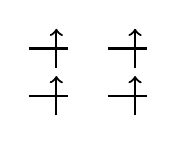
\begin{tikzpicture}
    % oberste MOs:
    \draw[thick] (0,0) -- (0.5,0); % erster Strich
    \draw[thick] (1,0) -- (1.5,0); % zweiter Strich
    % unterste MOs:
    \draw[thick] (0,-0.6) -- (0.5,-0.6); % dritter Strich
    \draw[thick] (1,-0.6) -- (1.5,-0.6); % vierter Strich
\draw[->, thick] (0.35, -0.25) -- (0.35, 0.25); 
\draw[->, thick] (1.35, -0.25) -- (1.35, 0.25); 
\draw[-> , thick] (0.35, -0.85) -- (0.35, -0.35); 
 \draw[-> , thick] (1.35, -0.85) -- (1.35, -0.35); 
\end{tikzpicture} \qquad 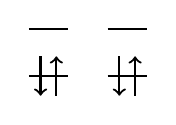
\begin{tikzpicture}
    % oberste MOs:
    \draw[thick] (0,0) -- (0.5,0); % erster Strich
    \draw[thick] (1,0) -- (1.5,0); % zweiter Strich
    % unterste MOs:
    \draw[thick] (0,-0.6) -- (0.5,-0.6); % dritter Strich
    \draw[thick] (1,-0.6) -- (1.5,-0.6); % vierter Strich
\draw[-> , thick] (0.35, -0.85) -- (0.35, -0.35); 
\draw[<- , thick] (0.15, -0.85) -- (0.15, -0.35); 
 \draw[-> , thick] (1.35, -0.85) -- (1.35, -0.35); 
\draw[<- , thick] (1.15, -0.85) -- (1.15, -0.35); 
\end{tikzpicture}}\right)-\left(\text{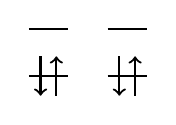
\begin{tikzpicture}
    % oberste MOs:
    \draw[thick] (0,0) -- (0.5,0); % erster Strich
    \draw[thick] (1,0) -- (1.5,0); % zweiter Strich
    % unterste MOs:
    \draw[thick] (0,-0.6) -- (0.5,-0.6); % dritter Strich
    \draw[thick] (1,-0.6) -- (1.5,-0.6); % vierter Strich
\draw[-> , thick] (0.35, -0.85) -- (0.35, -0.35); 
\draw[<- , thick] (0.15, -0.85) -- (0.15, -0.35); 
 \draw[-> , thick] (1.35, -0.85) -- (1.35, -0.35); 
\draw[<- , thick] (1.15, -0.85) -- (1.15, -0.35); 
\end{tikzpicture} \qquad 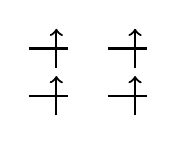
\begin{tikzpicture}
    % oberste MOs:
    \draw[thick] (0,0) -- (0.5,0); % erster Strich
    \draw[thick] (1,0) -- (1.5,0); % zweiter Strich
    % unterste MOs:
    \draw[thick] (0,-0.6) -- (0.5,-0.6); % dritter Strich
    \draw[thick] (1,-0.6) -- (1.5,-0.6); % vierter Strich
\draw[->, thick] (0.35, -0.25) -- (0.35, 0.25); 
\draw[->, thick] (1.35, -0.25) -- (1.35, 0.25); 
\draw[-> , thick] (0.35, -0.85) -- (0.35, -0.35); 
 \draw[-> , thick] (1.35, -0.85) -- (1.35, -0.35); 
\end{tikzpicture}}\right)\]enthaltene Monomer-Symmetrien = $a_{g}$\begin{multline*}=+\left(\left|(b_{1u}^{l}) \cdot (b_{2g}^{l}) \cdot (b_{3g}^{l}) \cdot (a_{u}^{l})\right|\right)-\left(\left|(b_{1u}^{r}) \cdot (b_{2g}^{r}) \cdot (b_{3g}^{r}) \cdot (a_{u}^{r})\right|\right)\end{multline*}
\begin{multline*}
=+2\left|\underbrace{\overbrace{a_{g} b_{3u} b_{2u} a_{u}}^{1 2 3 8}}_{b_{1u}}\right|-2\left|\underbrace{\overbrace{a_{g} b_{3u} b_{1g} b_{3g}}^{1 2 4 7}}_{b_{1u}}\right|+2\left|\underbrace{\overbrace{a_{g} b_{2u} b_{1g} b_{2g}}^{1 3 4 6}}_{b_{1u}}\right|+2\left|\underbrace{\overbrace{a_{g} b_{2g} b_{3g} a_{u}}^{1 6 7 8}}_{b_{1u}}\right|\\
-2\left|\underbrace{\overbrace{b_{3u} b_{2u} b_{1g} b_{1u}}^{2 3 4 5}}_{b_{1u}}\right|-2\left|\underbrace{\overbrace{b_{3u} b_{1u} b_{3g} a_{u}}^{2 5 7 8}}_{b_{1u}}\right|+2\left|\underbrace{\overbrace{b_{2u} b_{1u} b_{2g} a_{u}}^{3 5 6 8}}_{b_{1u}}\right|-2\left|\underbrace{\overbrace{b_{1g} b_{1u} b_{2g} b_{3g}}^{4 5 6 7}}_{b_{1u}}\right|
\end{multline*}
\\\\


\hrule\newpage 
\[ +\left(\text{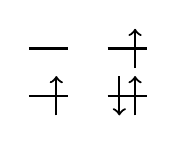
\begin{tikzpicture}
    % oberste MOs:
    \draw[thick] (0,0) -- (0.5,0); % erster Strich
    \draw[thick] (1,0) -- (1.5,0); % zweiter Strich
    % unterste MOs:
    \draw[thick] (0,-0.6) -- (0.5,-0.6); % dritter Strich
    \draw[thick] (1,-0.6) -- (1.5,-0.6); % vierter Strich
\draw[->, thick] (1.35, -0.25) -- (1.35, 0.25); 
\draw[-> , thick] (0.35, -0.85) -- (0.35, -0.35); 
 \draw[-> , thick] (1.35, -0.85) -- (1.35, -0.35); 
\draw[<- , thick] (1.15, -0.85) -- (1.15, -0.35); 
\end{tikzpicture} \qquad 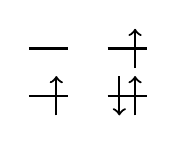
\begin{tikzpicture}
    % oberste MOs:
    \draw[thick] (0,0) -- (0.5,0); % erster Strich
    \draw[thick] (1,0) -- (1.5,0); % zweiter Strich
    % unterste MOs:
    \draw[thick] (0,-0.6) -- (0.5,-0.6); % dritter Strich
    \draw[thick] (1,-0.6) -- (1.5,-0.6); % vierter Strich
\draw[->, thick] (1.35, -0.25) -- (1.35, 0.25); 
\draw[-> , thick] (0.35, -0.85) -- (0.35, -0.35); 
 \draw[-> , thick] (1.35, -0.85) -- (1.35, -0.35); 
\draw[<- , thick] (1.15, -0.85) -- (1.15, -0.35); 
\end{tikzpicture}}\right)+\left(\text{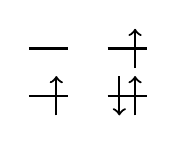
\begin{tikzpicture}
    % oberste MOs:
    \draw[thick] (0,0) -- (0.5,0); % erster Strich
    \draw[thick] (1,0) -- (1.5,0); % zweiter Strich
    % unterste MOs:
    \draw[thick] (0,-0.6) -- (0.5,-0.6); % dritter Strich
    \draw[thick] (1,-0.6) -- (1.5,-0.6); % vierter Strich
\draw[->, thick] (1.35, -0.25) -- (1.35, 0.25); 
\draw[-> , thick] (0.35, -0.85) -- (0.35, -0.35); 
 \draw[-> , thick] (1.35, -0.85) -- (1.35, -0.35); 
\draw[<- , thick] (1.15, -0.85) -- (1.15, -0.35); 
\end{tikzpicture} \qquad 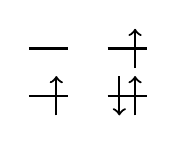
\begin{tikzpicture}
    % oberste MOs:
    \draw[thick] (0,0) -- (0.5,0); % erster Strich
    \draw[thick] (1,0) -- (1.5,0); % zweiter Strich
    % unterste MOs:
    \draw[thick] (0,-0.6) -- (0.5,-0.6); % dritter Strich
    \draw[thick] (1,-0.6) -- (1.5,-0.6); % vierter Strich
\draw[->, thick] (1.35, -0.25) -- (1.35, 0.25); 
\draw[-> , thick] (0.35, -0.85) -- (0.35, -0.35); 
 \draw[-> , thick] (1.35, -0.85) -- (1.35, -0.35); 
\draw[<- , thick] (1.15, -0.85) -- (1.15, -0.35); 
\end{tikzpicture}}\right)\]enthaltene Monomer-Symmetrien = $b_{2u}$\begin{multline*}=+\left(\left|(b_{2g}^{l}) \cdot (b_{2g}^{r}) \cdot (a_{u}^{l}) \cdot (a_{u}^{r})\right|\right)+\left(\left|(b_{2g}^{l}) \cdot (b_{2g}^{r}) \cdot (a_{u}^{l}) \cdot (a_{u}^{r})\right|\right)\end{multline*}
\begin{multline*}
=-8\left|\underbrace{\overbrace{b_{3u} b_{1g} b_{2g} a_{u}}^{2 4 6 8}}_{a_{g}}\right|
\end{multline*}
\\\\


\hrule\newpage 
\[ +\left(\text{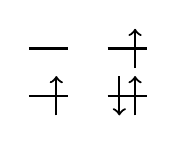
\begin{tikzpicture}
    % oberste MOs:
    \draw[thick] (0,0) -- (0.5,0); % erster Strich
    \draw[thick] (1,0) -- (1.5,0); % zweiter Strich
    % unterste MOs:
    \draw[thick] (0,-0.6) -- (0.5,-0.6); % dritter Strich
    \draw[thick] (1,-0.6) -- (1.5,-0.6); % vierter Strich
\draw[->, thick] (1.35, -0.25) -- (1.35, 0.25); 
\draw[-> , thick] (0.35, -0.85) -- (0.35, -0.35); 
 \draw[-> , thick] (1.35, -0.85) -- (1.35, -0.35); 
\draw[<- , thick] (1.15, -0.85) -- (1.15, -0.35); 
\end{tikzpicture} \qquad 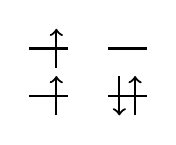
\begin{tikzpicture}
    % oberste MOs:
    \draw[thick] (0,0) -- (0.5,0); % erster Strich
    \draw[thick] (1,0) -- (1.5,0); % zweiter Strich
    % unterste MOs:
    \draw[thick] (0,-0.6) -- (0.5,-0.6); % dritter Strich
    \draw[thick] (1,-0.6) -- (1.5,-0.6); % vierter Strich
\draw[->, thick] (0.35, -0.25) -- (0.35, 0.25); 
\draw[-> , thick] (0.35, -0.85) -- (0.35, -0.35); 
 \draw[-> , thick] (1.35, -0.85) -- (1.35, -0.35); 
\draw[<- , thick] (1.15, -0.85) -- (1.15, -0.35); 
\end{tikzpicture}}\right)+\left(\text{\begin{tikzpicture}
    % oberste MOs:
    \draw[thick] (0,0) -- (0.5,0); % erster Strich
    \draw[thick] (1,0) -- (1.5,0); % zweiter Strich
    % unterste MOs:
    \draw[thick] (0,-0.6) -- (0.5,-0.6); % dritter Strich
    \draw[thick] (1,-0.6) -- (1.5,-0.6); % vierter Strich
\draw[->, thick] (0.35, -0.25) -- (0.35, 0.25); 
\draw[-> , thick] (0.35, -0.85) -- (0.35, -0.35); 
 \draw[-> , thick] (1.35, -0.85) -- (1.35, -0.35); 
\draw[<- , thick] (1.15, -0.85) -- (1.15, -0.35); 
\end{tikzpicture} \qquad \begin{tikzpicture}
    % oberste MOs:
    \draw[thick] (0,0) -- (0.5,0); % erster Strich
    \draw[thick] (1,0) -- (1.5,0); % zweiter Strich
    % unterste MOs:
    \draw[thick] (0,-0.6) -- (0.5,-0.6); % dritter Strich
    \draw[thick] (1,-0.6) -- (1.5,-0.6); % vierter Strich
\draw[->, thick] (1.35, -0.25) -- (1.35, 0.25); 
\draw[-> , thick] (0.35, -0.85) -- (0.35, -0.35); 
 \draw[-> , thick] (1.35, -0.85) -- (1.35, -0.35); 
\draw[<- , thick] (1.15, -0.85) -- (1.15, -0.35); 
\end{tikzpicture}}\right)\]enthaltene Monomer-Symmetrien = $b_{3u},b_{2u}$\begin{multline*}=+\left(\left|(b_{1u}^{r}) \cdot (b_{2g}^{l}) \cdot (b_{2g}^{r}) \cdot (a_{u}^{l})\right|\right)+\left(\left|(b_{1u}^{l}) \cdot (b_{2g}^{l}) \cdot (b_{2g}^{r}) \cdot (a_{u}^{r})\right|\right)\end{multline*}
\begin{multline*}
=+4\left|\underbrace{\overbrace{a_{g} b_{3u} b_{1g} b_{2g}}^{1 2 4 6}}_{a_{u}}\right|-4\left|\underbrace{\overbrace{b_{3u} b_{1u} b_{2g} a_{u}}^{2 5 6 8}}_{a_{u}}\right|
\end{multline*}
\\\\


\vspace{0.5cm}
\[ +\left(\text{\begin{tikzpicture}
    % oberste MOs:
    \draw[thick] (0,0) -- (0.5,0); % erster Strich
    \draw[thick] (1,0) -- (1.5,0); % zweiter Strich
    % unterste MOs:
    \draw[thick] (0,-0.6) -- (0.5,-0.6); % dritter Strich
    \draw[thick] (1,-0.6) -- (1.5,-0.6); % vierter Strich
\draw[->, thick] (1.35, -0.25) -- (1.35, 0.25); 
\draw[-> , thick] (0.35, -0.85) -- (0.35, -0.35); 
 \draw[-> , thick] (1.35, -0.85) -- (1.35, -0.35); 
\draw[<- , thick] (1.15, -0.85) -- (1.15, -0.35); 
\end{tikzpicture} \qquad \begin{tikzpicture}
    % oberste MOs:
    \draw[thick] (0,0) -- (0.5,0); % erster Strich
    \draw[thick] (1,0) -- (1.5,0); % zweiter Strich
    % unterste MOs:
    \draw[thick] (0,-0.6) -- (0.5,-0.6); % dritter Strich
    \draw[thick] (1,-0.6) -- (1.5,-0.6); % vierter Strich
\draw[->, thick] (0.35, -0.25) -- (0.35, 0.25); 
\draw[-> , thick] (0.35, -0.85) -- (0.35, -0.35); 
 \draw[-> , thick] (1.35, -0.85) -- (1.35, -0.35); 
\draw[<- , thick] (1.15, -0.85) -- (1.15, -0.35); 
\end{tikzpicture}}\right)-\left(\text{\begin{tikzpicture}
    % oberste MOs:
    \draw[thick] (0,0) -- (0.5,0); % erster Strich
    \draw[thick] (1,0) -- (1.5,0); % zweiter Strich
    % unterste MOs:
    \draw[thick] (0,-0.6) -- (0.5,-0.6); % dritter Strich
    \draw[thick] (1,-0.6) -- (1.5,-0.6); % vierter Strich
\draw[->, thick] (0.35, -0.25) -- (0.35, 0.25); 
\draw[-> , thick] (0.35, -0.85) -- (0.35, -0.35); 
 \draw[-> , thick] (1.35, -0.85) -- (1.35, -0.35); 
\draw[<- , thick] (1.15, -0.85) -- (1.15, -0.35); 
\end{tikzpicture} \qquad \begin{tikzpicture}
    % oberste MOs:
    \draw[thick] (0,0) -- (0.5,0); % erster Strich
    \draw[thick] (1,0) -- (1.5,0); % zweiter Strich
    % unterste MOs:
    \draw[thick] (0,-0.6) -- (0.5,-0.6); % dritter Strich
    \draw[thick] (1,-0.6) -- (1.5,-0.6); % vierter Strich
\draw[->, thick] (1.35, -0.25) -- (1.35, 0.25); 
\draw[-> , thick] (0.35, -0.85) -- (0.35, -0.35); 
 \draw[-> , thick] (1.35, -0.85) -- (1.35, -0.35); 
\draw[<- , thick] (1.15, -0.85) -- (1.15, -0.35); 
\end{tikzpicture}}\right)\]enthaltene Monomer-Symmetrien = $b_{3u},b_{2u}$\begin{multline*}=+\left(\left|(b_{1u}^{r}) \cdot (b_{2g}^{l}) \cdot (b_{2g}^{r}) \cdot (a_{u}^{l})\right|\right)-\left(\left|(b_{1u}^{l}) \cdot (b_{2g}^{l}) \cdot (b_{2g}^{r}) \cdot (a_{u}^{r})\right|\right)\end{multline*}
\begin{multline*}
=-4\left|\underbrace{\overbrace{a_{g} b_{3u} b_{2g} a_{u}}^{1 2 6 8}}_{b_{1g}}\right|-4\left|\underbrace{\overbrace{b_{3u} b_{1g} b_{1u} b_{2g}}^{2 4 5 6}}_{b_{1g}}\right|
\end{multline*}
\\\\


\hrule\newpage 
\[ +\left(\text{\begin{tikzpicture}
    % oberste MOs:
    \draw[thick] (0,0) -- (0.5,0); % erster Strich
    \draw[thick] (1,0) -- (1.5,0); % zweiter Strich
    % unterste MOs:
    \draw[thick] (0,-0.6) -- (0.5,-0.6); % dritter Strich
    \draw[thick] (1,-0.6) -- (1.5,-0.6); % vierter Strich
\draw[->, thick] (1.35, -0.25) -- (1.35, 0.25); 
\draw[-> , thick] (0.35, -0.85) -- (0.35, -0.35); 
 \draw[-> , thick] (1.35, -0.85) -- (1.35, -0.35); 
\draw[<- , thick] (1.15, -0.85) -- (1.15, -0.35); 
\end{tikzpicture} \qquad \begin{tikzpicture}
    % oberste MOs:
    \draw[thick] (0,0) -- (0.5,0); % erster Strich
    \draw[thick] (1,0) -- (1.5,0); % zweiter Strich
    % unterste MOs:
    \draw[thick] (0,-0.6) -- (0.5,-0.6); % dritter Strich
    \draw[thick] (1,-0.6) -- (1.5,-0.6); % vierter Strich
\draw[->, thick] (1.35, -0.25) -- (1.35, 0.25); 
\draw[-> , thick] (0.35, -0.85) -- (0.35, -0.35); 
\draw[<- , thick] (0.15, -0.85) -- (0.15, -0.35); 
 \draw[-> , thick] (1.35, -0.85) -- (1.35, -0.35); 
\end{tikzpicture}}\right)+\left(\text{\begin{tikzpicture}
    % oberste MOs:
    \draw[thick] (0,0) -- (0.5,0); % erster Strich
    \draw[thick] (1,0) -- (1.5,0); % zweiter Strich
    % unterste MOs:
    \draw[thick] (0,-0.6) -- (0.5,-0.6); % dritter Strich
    \draw[thick] (1,-0.6) -- (1.5,-0.6); % vierter Strich
\draw[->, thick] (1.35, -0.25) -- (1.35, 0.25); 
\draw[-> , thick] (0.35, -0.85) -- (0.35, -0.35); 
\draw[<- , thick] (0.15, -0.85) -- (0.15, -0.35); 
 \draw[-> , thick] (1.35, -0.85) -- (1.35, -0.35); 
\end{tikzpicture} \qquad \begin{tikzpicture}
    % oberste MOs:
    \draw[thick] (0,0) -- (0.5,0); % erster Strich
    \draw[thick] (1,0) -- (1.5,0); % zweiter Strich
    % unterste MOs:
    \draw[thick] (0,-0.6) -- (0.5,-0.6); % dritter Strich
    \draw[thick] (1,-0.6) -- (1.5,-0.6); % vierter Strich
\draw[->, thick] (1.35, -0.25) -- (1.35, 0.25); 
\draw[-> , thick] (0.35, -0.85) -- (0.35, -0.35); 
 \draw[-> , thick] (1.35, -0.85) -- (1.35, -0.35); 
\draw[<- , thick] (1.15, -0.85) -- (1.15, -0.35); 
\end{tikzpicture}}\right)\]enthaltene Monomer-Symmetrien = $b_{3u},b_{2u}$\begin{multline*}=+\left(\left|(b_{2g}^{l}) \cdot (b_{3g}^{r}) \cdot (a_{u}^{l}) \cdot (a_{u}^{r})\right|\right)+\left(\left|(b_{2g}^{r}) \cdot (b_{3g}^{l}) \cdot (a_{u}^{l}) \cdot (a_{u}^{r})\right|\right)\end{multline*}
\begin{multline*}
=-4\left|\underbrace{\overbrace{b_{3u} b_{2u} b_{1g} a_{u}}^{2 3 4 8}}_{a_{u}}\right|+4\left|\underbrace{\overbrace{b_{1g} b_{2g} b_{3g} a_{u}}^{4 6 7 8}}_{a_{u}}\right|
\end{multline*}
\\\\


\vspace{0.5cm}
\[ +\left(\text{\begin{tikzpicture}
    % oberste MOs:
    \draw[thick] (0,0) -- (0.5,0); % erster Strich
    \draw[thick] (1,0) -- (1.5,0); % zweiter Strich
    % unterste MOs:
    \draw[thick] (0,-0.6) -- (0.5,-0.6); % dritter Strich
    \draw[thick] (1,-0.6) -- (1.5,-0.6); % vierter Strich
\draw[->, thick] (1.35, -0.25) -- (1.35, 0.25); 
\draw[-> , thick] (0.35, -0.85) -- (0.35, -0.35); 
 \draw[-> , thick] (1.35, -0.85) -- (1.35, -0.35); 
\draw[<- , thick] (1.15, -0.85) -- (1.15, -0.35); 
\end{tikzpicture} \qquad \begin{tikzpicture}
    % oberste MOs:
    \draw[thick] (0,0) -- (0.5,0); % erster Strich
    \draw[thick] (1,0) -- (1.5,0); % zweiter Strich
    % unterste MOs:
    \draw[thick] (0,-0.6) -- (0.5,-0.6); % dritter Strich
    \draw[thick] (1,-0.6) -- (1.5,-0.6); % vierter Strich
\draw[->, thick] (1.35, -0.25) -- (1.35, 0.25); 
\draw[-> , thick] (0.35, -0.85) -- (0.35, -0.35); 
\draw[<- , thick] (0.15, -0.85) -- (0.15, -0.35); 
 \draw[-> , thick] (1.35, -0.85) -- (1.35, -0.35); 
\end{tikzpicture}}\right)-\left(\text{\begin{tikzpicture}
    % oberste MOs:
    \draw[thick] (0,0) -- (0.5,0); % erster Strich
    \draw[thick] (1,0) -- (1.5,0); % zweiter Strich
    % unterste MOs:
    \draw[thick] (0,-0.6) -- (0.5,-0.6); % dritter Strich
    \draw[thick] (1,-0.6) -- (1.5,-0.6); % vierter Strich
\draw[->, thick] (1.35, -0.25) -- (1.35, 0.25); 
\draw[-> , thick] (0.35, -0.85) -- (0.35, -0.35); 
\draw[<- , thick] (0.15, -0.85) -- (0.15, -0.35); 
 \draw[-> , thick] (1.35, -0.85) -- (1.35, -0.35); 
\end{tikzpicture} \qquad \begin{tikzpicture}
    % oberste MOs:
    \draw[thick] (0,0) -- (0.5,0); % erster Strich
    \draw[thick] (1,0) -- (1.5,0); % zweiter Strich
    % unterste MOs:
    \draw[thick] (0,-0.6) -- (0.5,-0.6); % dritter Strich
    \draw[thick] (1,-0.6) -- (1.5,-0.6); % vierter Strich
\draw[->, thick] (1.35, -0.25) -- (1.35, 0.25); 
\draw[-> , thick] (0.35, -0.85) -- (0.35, -0.35); 
 \draw[-> , thick] (1.35, -0.85) -- (1.35, -0.35); 
\draw[<- , thick] (1.15, -0.85) -- (1.15, -0.35); 
\end{tikzpicture}}\right)\]enthaltene Monomer-Symmetrien = $b_{3u},b_{2u}$\begin{multline*}=+\left(\left|(b_{2g}^{l}) \cdot (b_{3g}^{r}) \cdot (a_{u}^{l}) \cdot (a_{u}^{r})\right|\right)-\left(\left|(b_{2g}^{r}) \cdot (b_{3g}^{l}) \cdot (a_{u}^{l}) \cdot (a_{u}^{r})\right|\right)\end{multline*}
\begin{multline*}
=-4\left|\underbrace{\overbrace{b_{3u} b_{1g} b_{3g} a_{u}}^{2 4 7 8}}_{b_{1g}}\right|-4\left|\underbrace{\overbrace{b_{2u} b_{1g} b_{2g} a_{u}}^{3 4 6 8}}_{b_{1g}}\right|
\end{multline*}
\\\\


\hrule\newpage 
\[ +\left(\text{\begin{tikzpicture}
    % oberste MOs:
    \draw[thick] (0,0) -- (0.5,0); % erster Strich
    \draw[thick] (1,0) -- (1.5,0); % zweiter Strich
    % unterste MOs:
    \draw[thick] (0,-0.6) -- (0.5,-0.6); % dritter Strich
    \draw[thick] (1,-0.6) -- (1.5,-0.6); % vierter Strich
\draw[->, thick] (1.35, -0.25) -- (1.35, 0.25); 
\draw[-> , thick] (0.35, -0.85) -- (0.35, -0.35); 
 \draw[-> , thick] (1.35, -0.85) -- (1.35, -0.35); 
\draw[<- , thick] (1.15, -0.85) -- (1.15, -0.35); 
\end{tikzpicture} \qquad \begin{tikzpicture}
    % oberste MOs:
    \draw[thick] (0,0) -- (0.5,0); % erster Strich
    \draw[thick] (1,0) -- (1.5,0); % zweiter Strich
    % unterste MOs:
    \draw[thick] (0,-0.6) -- (0.5,-0.6); % dritter Strich
    \draw[thick] (1,-0.6) -- (1.5,-0.6); % vierter Strich
\draw[->, thick] (0.35, -0.25) -- (0.35, 0.25); 
\draw[-> , thick] (0.35, -0.85) -- (0.35, -0.35); 
\draw[<- , thick] (0.15, -0.85) -- (0.15, -0.35); 
 \draw[-> , thick] (1.35, -0.85) -- (1.35, -0.35); 
\end{tikzpicture}}\right)+\left(\text{\begin{tikzpicture}
    % oberste MOs:
    \draw[thick] (0,0) -- (0.5,0); % erster Strich
    \draw[thick] (1,0) -- (1.5,0); % zweiter Strich
    % unterste MOs:
    \draw[thick] (0,-0.6) -- (0.5,-0.6); % dritter Strich
    \draw[thick] (1,-0.6) -- (1.5,-0.6); % vierter Strich
\draw[->, thick] (0.35, -0.25) -- (0.35, 0.25); 
\draw[-> , thick] (0.35, -0.85) -- (0.35, -0.35); 
\draw[<- , thick] (0.15, -0.85) -- (0.15, -0.35); 
 \draw[-> , thick] (1.35, -0.85) -- (1.35, -0.35); 
\end{tikzpicture} \qquad \begin{tikzpicture}
    % oberste MOs:
    \draw[thick] (0,0) -- (0.5,0); % erster Strich
    \draw[thick] (1,0) -- (1.5,0); % zweiter Strich
    % unterste MOs:
    \draw[thick] (0,-0.6) -- (0.5,-0.6); % dritter Strich
    \draw[thick] (1,-0.6) -- (1.5,-0.6); % vierter Strich
\draw[->, thick] (1.35, -0.25) -- (1.35, 0.25); 
\draw[-> , thick] (0.35, -0.85) -- (0.35, -0.35); 
 \draw[-> , thick] (1.35, -0.85) -- (1.35, -0.35); 
\draw[<- , thick] (1.15, -0.85) -- (1.15, -0.35); 
\end{tikzpicture}}\right)\]enthaltene Monomer-Symmetrien = $b_{2u}$\begin{multline*}=+\left(\left|(b_{1u}^{r}) \cdot (b_{2g}^{l}) \cdot (b_{3g}^{r}) \cdot (a_{u}^{l})\right|\right)+\left(\left|(b_{1u}^{l}) \cdot (b_{2g}^{r}) \cdot (b_{3g}^{l}) \cdot (a_{u}^{r})\right|\right)\end{multline*}
\begin{multline*}
=+2\left|\underbrace{\overbrace{a_{g} b_{3u} b_{2u} b_{1g}}^{1 2 3 4}}_{a_{g}}\right|-2\left|\underbrace{\overbrace{a_{g} b_{3u} b_{3g} a_{u}}^{1 2 7 8}}_{a_{g}}\right|-2\left|\underbrace{\overbrace{a_{g} b_{2u} b_{2g} a_{u}}^{1 3 6 8}}_{a_{g}}\right|-2\left|\underbrace{\overbrace{a_{g} b_{1g} b_{2g} b_{3g}}^{1 4 6 7}}_{a_{g}}\right|\\
-2\left|\underbrace{\overbrace{b_{3u} b_{2u} b_{1u} a_{u}}^{2 3 5 8}}_{a_{g}}\right|-2\left|\underbrace{\overbrace{b_{3u} b_{1g} b_{1u} b_{3g}}^{2 4 5 7}}_{a_{g}}\right|-2\left|\underbrace{\overbrace{b_{2u} b_{1g} b_{1u} b_{2g}}^{3 4 5 6}}_{a_{g}}\right|+2\left|\underbrace{\overbrace{b_{1u} b_{2g} b_{3g} a_{u}}^{5 6 7 8}}_{a_{g}}\right|
\end{multline*}
\\\\


\vspace{0.5cm}
\[ +\left(\text{\begin{tikzpicture}
    % oberste MOs:
    \draw[thick] (0,0) -- (0.5,0); % erster Strich
    \draw[thick] (1,0) -- (1.5,0); % zweiter Strich
    % unterste MOs:
    \draw[thick] (0,-0.6) -- (0.5,-0.6); % dritter Strich
    \draw[thick] (1,-0.6) -- (1.5,-0.6); % vierter Strich
\draw[->, thick] (1.35, -0.25) -- (1.35, 0.25); 
\draw[-> , thick] (0.35, -0.85) -- (0.35, -0.35); 
 \draw[-> , thick] (1.35, -0.85) -- (1.35, -0.35); 
\draw[<- , thick] (1.15, -0.85) -- (1.15, -0.35); 
\end{tikzpicture} \qquad \begin{tikzpicture}
    % oberste MOs:
    \draw[thick] (0,0) -- (0.5,0); % erster Strich
    \draw[thick] (1,0) -- (1.5,0); % zweiter Strich
    % unterste MOs:
    \draw[thick] (0,-0.6) -- (0.5,-0.6); % dritter Strich
    \draw[thick] (1,-0.6) -- (1.5,-0.6); % vierter Strich
\draw[->, thick] (0.35, -0.25) -- (0.35, 0.25); 
\draw[-> , thick] (0.35, -0.85) -- (0.35, -0.35); 
\draw[<- , thick] (0.15, -0.85) -- (0.15, -0.35); 
 \draw[-> , thick] (1.35, -0.85) -- (1.35, -0.35); 
\end{tikzpicture}}\right)-\left(\text{\begin{tikzpicture}
    % oberste MOs:
    \draw[thick] (0,0) -- (0.5,0); % erster Strich
    \draw[thick] (1,0) -- (1.5,0); % zweiter Strich
    % unterste MOs:
    \draw[thick] (0,-0.6) -- (0.5,-0.6); % dritter Strich
    \draw[thick] (1,-0.6) -- (1.5,-0.6); % vierter Strich
\draw[->, thick] (0.35, -0.25) -- (0.35, 0.25); 
\draw[-> , thick] (0.35, -0.85) -- (0.35, -0.35); 
\draw[<- , thick] (0.15, -0.85) -- (0.15, -0.35); 
 \draw[-> , thick] (1.35, -0.85) -- (1.35, -0.35); 
\end{tikzpicture} \qquad \begin{tikzpicture}
    % oberste MOs:
    \draw[thick] (0,0) -- (0.5,0); % erster Strich
    \draw[thick] (1,0) -- (1.5,0); % zweiter Strich
    % unterste MOs:
    \draw[thick] (0,-0.6) -- (0.5,-0.6); % dritter Strich
    \draw[thick] (1,-0.6) -- (1.5,-0.6); % vierter Strich
\draw[->, thick] (1.35, -0.25) -- (1.35, 0.25); 
\draw[-> , thick] (0.35, -0.85) -- (0.35, -0.35); 
 \draw[-> , thick] (1.35, -0.85) -- (1.35, -0.35); 
\draw[<- , thick] (1.15, -0.85) -- (1.15, -0.35); 
\end{tikzpicture}}\right)\]enthaltene Monomer-Symmetrien = $b_{2u}$\begin{multline*}=+\left(\left|(b_{1u}^{r}) \cdot (b_{2g}^{l}) \cdot (b_{3g}^{r}) \cdot (a_{u}^{l})\right|\right)-\left(\left|(b_{1u}^{l}) \cdot (b_{2g}^{r}) \cdot (b_{3g}^{l}) \cdot (a_{u}^{r})\right|\right)\end{multline*}
\begin{multline*}
=+2\left|\underbrace{\overbrace{a_{g} b_{3u} b_{2u} a_{u}}^{1 2 3 8}}_{b_{1u}}\right|+2\left|\underbrace{\overbrace{a_{g} b_{3u} b_{1g} b_{3g}}^{1 2 4 7}}_{b_{1u}}\right|+2\left|\underbrace{\overbrace{a_{g} b_{2u} b_{1g} b_{2g}}^{1 3 4 6}}_{b_{1u}}\right|-2\left|\underbrace{\overbrace{a_{g} b_{2g} b_{3g} a_{u}}^{1 6 7 8}}_{b_{1u}}\right|\\
+2\left|\underbrace{\overbrace{b_{3u} b_{2u} b_{1g} b_{1u}}^{2 3 4 5}}_{b_{1u}}\right|-2\left|\underbrace{\overbrace{b_{3u} b_{1u} b_{3g} a_{u}}^{2 5 7 8}}_{b_{1u}}\right|-2\left|\underbrace{\overbrace{b_{2u} b_{1u} b_{2g} a_{u}}^{3 5 6 8}}_{b_{1u}}\right|-2\left|\underbrace{\overbrace{b_{1g} b_{1u} b_{2g} b_{3g}}^{4 5 6 7}}_{b_{1u}}\right|
\end{multline*}
\\\\


\hrule\newpage 
\[ +\left(\text{\begin{tikzpicture}
    % oberste MOs:
    \draw[thick] (0,0) -- (0.5,0); % erster Strich
    \draw[thick] (1,0) -- (1.5,0); % zweiter Strich
    % unterste MOs:
    \draw[thick] (0,-0.6) -- (0.5,-0.6); % dritter Strich
    \draw[thick] (1,-0.6) -- (1.5,-0.6); % vierter Strich
\draw[->, thick] (0.35, -0.25) -- (0.35, 0.25); 
\draw[-> , thick] (0.35, -0.85) -- (0.35, -0.35); 
 \draw[-> , thick] (1.35, -0.85) -- (1.35, -0.35); 
\draw[<- , thick] (1.15, -0.85) -- (1.15, -0.35); 
\end{tikzpicture} \qquad \begin{tikzpicture}
    % oberste MOs:
    \draw[thick] (0,0) -- (0.5,0); % erster Strich
    \draw[thick] (1,0) -- (1.5,0); % zweiter Strich
    % unterste MOs:
    \draw[thick] (0,-0.6) -- (0.5,-0.6); % dritter Strich
    \draw[thick] (1,-0.6) -- (1.5,-0.6); % vierter Strich
\draw[->, thick] (0.35, -0.25) -- (0.35, 0.25); 
\draw[-> , thick] (0.35, -0.85) -- (0.35, -0.35); 
 \draw[-> , thick] (1.35, -0.85) -- (1.35, -0.35); 
\draw[<- , thick] (1.15, -0.85) -- (1.15, -0.35); 
\end{tikzpicture}}\right)+\left(\text{\begin{tikzpicture}
    % oberste MOs:
    \draw[thick] (0,0) -- (0.5,0); % erster Strich
    \draw[thick] (1,0) -- (1.5,0); % zweiter Strich
    % unterste MOs:
    \draw[thick] (0,-0.6) -- (0.5,-0.6); % dritter Strich
    \draw[thick] (1,-0.6) -- (1.5,-0.6); % vierter Strich
\draw[->, thick] (0.35, -0.25) -- (0.35, 0.25); 
\draw[-> , thick] (0.35, -0.85) -- (0.35, -0.35); 
 \draw[-> , thick] (1.35, -0.85) -- (1.35, -0.35); 
\draw[<- , thick] (1.15, -0.85) -- (1.15, -0.35); 
\end{tikzpicture} \qquad \begin{tikzpicture}
    % oberste MOs:
    \draw[thick] (0,0) -- (0.5,0); % erster Strich
    \draw[thick] (1,0) -- (1.5,0); % zweiter Strich
    % unterste MOs:
    \draw[thick] (0,-0.6) -- (0.5,-0.6); % dritter Strich
    \draw[thick] (1,-0.6) -- (1.5,-0.6); % vierter Strich
\draw[->, thick] (0.35, -0.25) -- (0.35, 0.25); 
\draw[-> , thick] (0.35, -0.85) -- (0.35, -0.35); 
 \draw[-> , thick] (1.35, -0.85) -- (1.35, -0.35); 
\draw[<- , thick] (1.15, -0.85) -- (1.15, -0.35); 
\end{tikzpicture}}\right)\]enthaltene Monomer-Symmetrien = $b_{3u}$\begin{multline*}=+\left(\left|(b_{1u}^{l}) \cdot (b_{1u}^{r}) \cdot (b_{2g}^{l}) \cdot (b_{2g}^{r})\right|\right)+\left(\left|(b_{1u}^{l}) \cdot (b_{1u}^{r}) \cdot (b_{2g}^{l}) \cdot (b_{2g}^{r})\right|\right)\end{multline*}
\begin{multline*}
=-8\left|\underbrace{\overbrace{a_{g} b_{3u} b_{1u} b_{2g}}^{1 2 5 6}}_{a_{g}}\right|
\end{multline*}
\\\\


\hrule\newpage 
\[ +\left(\text{\begin{tikzpicture}
    % oberste MOs:
    \draw[thick] (0,0) -- (0.5,0); % erster Strich
    \draw[thick] (1,0) -- (1.5,0); % zweiter Strich
    % unterste MOs:
    \draw[thick] (0,-0.6) -- (0.5,-0.6); % dritter Strich
    \draw[thick] (1,-0.6) -- (1.5,-0.6); % vierter Strich
\draw[->, thick] (0.35, -0.25) -- (0.35, 0.25); 
\draw[-> , thick] (0.35, -0.85) -- (0.35, -0.35); 
 \draw[-> , thick] (1.35, -0.85) -- (1.35, -0.35); 
\draw[<- , thick] (1.15, -0.85) -- (1.15, -0.35); 
\end{tikzpicture} \qquad \begin{tikzpicture}
    % oberste MOs:
    \draw[thick] (0,0) -- (0.5,0); % erster Strich
    \draw[thick] (1,0) -- (1.5,0); % zweiter Strich
    % unterste MOs:
    \draw[thick] (0,-0.6) -- (0.5,-0.6); % dritter Strich
    \draw[thick] (1,-0.6) -- (1.5,-0.6); % vierter Strich
\draw[->, thick] (1.35, -0.25) -- (1.35, 0.25); 
\draw[-> , thick] (0.35, -0.85) -- (0.35, -0.35); 
\draw[<- , thick] (0.15, -0.85) -- (0.15, -0.35); 
 \draw[-> , thick] (1.35, -0.85) -- (1.35, -0.35); 
\end{tikzpicture}}\right)+\left(\text{\begin{tikzpicture}
    % oberste MOs:
    \draw[thick] (0,0) -- (0.5,0); % erster Strich
    \draw[thick] (1,0) -- (1.5,0); % zweiter Strich
    % unterste MOs:
    \draw[thick] (0,-0.6) -- (0.5,-0.6); % dritter Strich
    \draw[thick] (1,-0.6) -- (1.5,-0.6); % vierter Strich
\draw[->, thick] (1.35, -0.25) -- (1.35, 0.25); 
\draw[-> , thick] (0.35, -0.85) -- (0.35, -0.35); 
\draw[<- , thick] (0.15, -0.85) -- (0.15, -0.35); 
 \draw[-> , thick] (1.35, -0.85) -- (1.35, -0.35); 
\end{tikzpicture} \qquad \begin{tikzpicture}
    % oberste MOs:
    \draw[thick] (0,0) -- (0.5,0); % erster Strich
    \draw[thick] (1,0) -- (1.5,0); % zweiter Strich
    % unterste MOs:
    \draw[thick] (0,-0.6) -- (0.5,-0.6); % dritter Strich
    \draw[thick] (1,-0.6) -- (1.5,-0.6); % vierter Strich
\draw[->, thick] (0.35, -0.25) -- (0.35, 0.25); 
\draw[-> , thick] (0.35, -0.85) -- (0.35, -0.35); 
 \draw[-> , thick] (1.35, -0.85) -- (1.35, -0.35); 
\draw[<- , thick] (1.15, -0.85) -- (1.15, -0.35); 
\end{tikzpicture}}\right)\]enthaltene Monomer-Symmetrien = $b_{3u}$\begin{multline*}=+\left(\left|(b_{1u}^{l}) \cdot (b_{2g}^{l}) \cdot (b_{3g}^{r}) \cdot (a_{u}^{r})\right|\right)+\left(\left|(b_{1u}^{r}) \cdot (b_{2g}^{r}) \cdot (b_{3g}^{l}) \cdot (a_{u}^{l})\right|\right)\end{multline*}
\begin{multline*}
=+2\left|\underbrace{\overbrace{a_{g} b_{3u} b_{2u} b_{1g}}^{1 2 3 4}}_{a_{g}}\right|+2\left|\underbrace{\overbrace{a_{g} b_{3u} b_{3g} a_{u}}^{1 2 7 8}}_{a_{g}}\right|+2\left|\underbrace{\overbrace{a_{g} b_{2u} b_{2g} a_{u}}^{1 3 6 8}}_{a_{g}}\right|-2\left|\underbrace{\overbrace{a_{g} b_{1g} b_{2g} b_{3g}}^{1 4 6 7}}_{a_{g}}\right|\\
-2\left|\underbrace{\overbrace{b_{3u} b_{2u} b_{1u} a_{u}}^{2 3 5 8}}_{a_{g}}\right|+2\left|\underbrace{\overbrace{b_{3u} b_{1g} b_{1u} b_{3g}}^{2 4 5 7}}_{a_{g}}\right|+2\left|\underbrace{\overbrace{b_{2u} b_{1g} b_{1u} b_{2g}}^{3 4 5 6}}_{a_{g}}\right|+2\left|\underbrace{\overbrace{b_{1u} b_{2g} b_{3g} a_{u}}^{5 6 7 8}}_{a_{g}}\right|
\end{multline*}
\\\\


\vspace{0.5cm}
\[ +\left(\text{\begin{tikzpicture}
    % oberste MOs:
    \draw[thick] (0,0) -- (0.5,0); % erster Strich
    \draw[thick] (1,0) -- (1.5,0); % zweiter Strich
    % unterste MOs:
    \draw[thick] (0,-0.6) -- (0.5,-0.6); % dritter Strich
    \draw[thick] (1,-0.6) -- (1.5,-0.6); % vierter Strich
\draw[->, thick] (0.35, -0.25) -- (0.35, 0.25); 
\draw[-> , thick] (0.35, -0.85) -- (0.35, -0.35); 
 \draw[-> , thick] (1.35, -0.85) -- (1.35, -0.35); 
\draw[<- , thick] (1.15, -0.85) -- (1.15, -0.35); 
\end{tikzpicture} \qquad \begin{tikzpicture}
    % oberste MOs:
    \draw[thick] (0,0) -- (0.5,0); % erster Strich
    \draw[thick] (1,0) -- (1.5,0); % zweiter Strich
    % unterste MOs:
    \draw[thick] (0,-0.6) -- (0.5,-0.6); % dritter Strich
    \draw[thick] (1,-0.6) -- (1.5,-0.6); % vierter Strich
\draw[->, thick] (1.35, -0.25) -- (1.35, 0.25); 
\draw[-> , thick] (0.35, -0.85) -- (0.35, -0.35); 
\draw[<- , thick] (0.15, -0.85) -- (0.15, -0.35); 
 \draw[-> , thick] (1.35, -0.85) -- (1.35, -0.35); 
\end{tikzpicture}}\right)-\left(\text{\begin{tikzpicture}
    % oberste MOs:
    \draw[thick] (0,0) -- (0.5,0); % erster Strich
    \draw[thick] (1,0) -- (1.5,0); % zweiter Strich
    % unterste MOs:
    \draw[thick] (0,-0.6) -- (0.5,-0.6); % dritter Strich
    \draw[thick] (1,-0.6) -- (1.5,-0.6); % vierter Strich
\draw[->, thick] (1.35, -0.25) -- (1.35, 0.25); 
\draw[-> , thick] (0.35, -0.85) -- (0.35, -0.35); 
\draw[<- , thick] (0.15, -0.85) -- (0.15, -0.35); 
 \draw[-> , thick] (1.35, -0.85) -- (1.35, -0.35); 
\end{tikzpicture} \qquad \begin{tikzpicture}
    % oberste MOs:
    \draw[thick] (0,0) -- (0.5,0); % erster Strich
    \draw[thick] (1,0) -- (1.5,0); % zweiter Strich
    % unterste MOs:
    \draw[thick] (0,-0.6) -- (0.5,-0.6); % dritter Strich
    \draw[thick] (1,-0.6) -- (1.5,-0.6); % vierter Strich
\draw[->, thick] (0.35, -0.25) -- (0.35, 0.25); 
\draw[-> , thick] (0.35, -0.85) -- (0.35, -0.35); 
 \draw[-> , thick] (1.35, -0.85) -- (1.35, -0.35); 
\draw[<- , thick] (1.15, -0.85) -- (1.15, -0.35); 
\end{tikzpicture}}\right)\]enthaltene Monomer-Symmetrien = $b_{3u}$\begin{multline*}=+\left(\left|(b_{1u}^{l}) \cdot (b_{2g}^{l}) \cdot (b_{3g}^{r}) \cdot (a_{u}^{r})\right|\right)-\left(\left|(b_{1u}^{r}) \cdot (b_{2g}^{r}) \cdot (b_{3g}^{l}) \cdot (a_{u}^{l})\right|\right)\end{multline*}
\begin{multline*}
=-2\left|\underbrace{\overbrace{a_{g} b_{3u} b_{2u} a_{u}}^{1 2 3 8}}_{b_{1u}}\right|+2\left|\underbrace{\overbrace{a_{g} b_{3u} b_{1g} b_{3g}}^{1 2 4 7}}_{b_{1u}}\right|+2\left|\underbrace{\overbrace{a_{g} b_{2u} b_{1g} b_{2g}}^{1 3 4 6}}_{b_{1u}}\right|+2\left|\underbrace{\overbrace{a_{g} b_{2g} b_{3g} a_{u}}^{1 6 7 8}}_{b_{1u}}\right|\\
-2\left|\underbrace{\overbrace{b_{3u} b_{2u} b_{1g} b_{1u}}^{2 3 4 5}}_{b_{1u}}\right|-2\left|\underbrace{\overbrace{b_{3u} b_{1u} b_{3g} a_{u}}^{2 5 7 8}}_{b_{1u}}\right|-2\left|\underbrace{\overbrace{b_{2u} b_{1u} b_{2g} a_{u}}^{3 5 6 8}}_{b_{1u}}\right|+2\left|\underbrace{\overbrace{b_{1g} b_{1u} b_{2g} b_{3g}}^{4 5 6 7}}_{b_{1u}}\right|
\end{multline*}
\\\\


\hrule\newpage 
\[ +\left(\text{\begin{tikzpicture}
    % oberste MOs:
    \draw[thick] (0,0) -- (0.5,0); % erster Strich
    \draw[thick] (1,0) -- (1.5,0); % zweiter Strich
    % unterste MOs:
    \draw[thick] (0,-0.6) -- (0.5,-0.6); % dritter Strich
    \draw[thick] (1,-0.6) -- (1.5,-0.6); % vierter Strich
\draw[->, thick] (0.35, -0.25) -- (0.35, 0.25); 
\draw[-> , thick] (0.35, -0.85) -- (0.35, -0.35); 
 \draw[-> , thick] (1.35, -0.85) -- (1.35, -0.35); 
\draw[<- , thick] (1.15, -0.85) -- (1.15, -0.35); 
\end{tikzpicture} \qquad \begin{tikzpicture}
    % oberste MOs:
    \draw[thick] (0,0) -- (0.5,0); % erster Strich
    \draw[thick] (1,0) -- (1.5,0); % zweiter Strich
    % unterste MOs:
    \draw[thick] (0,-0.6) -- (0.5,-0.6); % dritter Strich
    \draw[thick] (1,-0.6) -- (1.5,-0.6); % vierter Strich
\draw[->, thick] (0.35, -0.25) -- (0.35, 0.25); 
\draw[-> , thick] (0.35, -0.85) -- (0.35, -0.35); 
\draw[<- , thick] (0.15, -0.85) -- (0.15, -0.35); 
 \draw[-> , thick] (1.35, -0.85) -- (1.35, -0.35); 
\end{tikzpicture}}\right)+\left(\text{\begin{tikzpicture}
    % oberste MOs:
    \draw[thick] (0,0) -- (0.5,0); % erster Strich
    \draw[thick] (1,0) -- (1.5,0); % zweiter Strich
    % unterste MOs:
    \draw[thick] (0,-0.6) -- (0.5,-0.6); % dritter Strich
    \draw[thick] (1,-0.6) -- (1.5,-0.6); % vierter Strich
\draw[->, thick] (0.35, -0.25) -- (0.35, 0.25); 
\draw[-> , thick] (0.35, -0.85) -- (0.35, -0.35); 
\draw[<- , thick] (0.15, -0.85) -- (0.15, -0.35); 
 \draw[-> , thick] (1.35, -0.85) -- (1.35, -0.35); 
\end{tikzpicture} \qquad \begin{tikzpicture}
    % oberste MOs:
    \draw[thick] (0,0) -- (0.5,0); % erster Strich
    \draw[thick] (1,0) -- (1.5,0); % zweiter Strich
    % unterste MOs:
    \draw[thick] (0,-0.6) -- (0.5,-0.6); % dritter Strich
    \draw[thick] (1,-0.6) -- (1.5,-0.6); % vierter Strich
\draw[->, thick] (0.35, -0.25) -- (0.35, 0.25); 
\draw[-> , thick] (0.35, -0.85) -- (0.35, -0.35); 
 \draw[-> , thick] (1.35, -0.85) -- (1.35, -0.35); 
\draw[<- , thick] (1.15, -0.85) -- (1.15, -0.35); 
\end{tikzpicture}}\right)\]enthaltene Monomer-Symmetrien = $b_{3u},b_{2u}$\begin{multline*}=+\left(\left|(b_{1u}^{l}) \cdot (b_{1u}^{r}) \cdot (b_{2g}^{l}) \cdot (b_{3g}^{r})\right|\right)+\left(\left|(b_{1u}^{l}) \cdot (b_{1u}^{r}) \cdot (b_{2g}^{r}) \cdot (b_{3g}^{l})\right|\right)\end{multline*}
\begin{multline*}
=-4\left|\underbrace{\overbrace{a_{g} b_{3u} b_{2u} b_{1u}}^{1 2 3 5}}_{a_{u}}\right|+4\left|\underbrace{\overbrace{a_{g} b_{1u} b_{2g} b_{3g}}^{1 5 6 7}}_{a_{u}}\right|
\end{multline*}
\\\\


\vspace{0.5cm}
\[ +\left(\text{\begin{tikzpicture}
    % oberste MOs:
    \draw[thick] (0,0) -- (0.5,0); % erster Strich
    \draw[thick] (1,0) -- (1.5,0); % zweiter Strich
    % unterste MOs:
    \draw[thick] (0,-0.6) -- (0.5,-0.6); % dritter Strich
    \draw[thick] (1,-0.6) -- (1.5,-0.6); % vierter Strich
\draw[->, thick] (0.35, -0.25) -- (0.35, 0.25); 
\draw[-> , thick] (0.35, -0.85) -- (0.35, -0.35); 
 \draw[-> , thick] (1.35, -0.85) -- (1.35, -0.35); 
\draw[<- , thick] (1.15, -0.85) -- (1.15, -0.35); 
\end{tikzpicture} \qquad \begin{tikzpicture}
    % oberste MOs:
    \draw[thick] (0,0) -- (0.5,0); % erster Strich
    \draw[thick] (1,0) -- (1.5,0); % zweiter Strich
    % unterste MOs:
    \draw[thick] (0,-0.6) -- (0.5,-0.6); % dritter Strich
    \draw[thick] (1,-0.6) -- (1.5,-0.6); % vierter Strich
\draw[->, thick] (0.35, -0.25) -- (0.35, 0.25); 
\draw[-> , thick] (0.35, -0.85) -- (0.35, -0.35); 
\draw[<- , thick] (0.15, -0.85) -- (0.15, -0.35); 
 \draw[-> , thick] (1.35, -0.85) -- (1.35, -0.35); 
\end{tikzpicture}}\right)-\left(\text{\begin{tikzpicture}
    % oberste MOs:
    \draw[thick] (0,0) -- (0.5,0); % erster Strich
    \draw[thick] (1,0) -- (1.5,0); % zweiter Strich
    % unterste MOs:
    \draw[thick] (0,-0.6) -- (0.5,-0.6); % dritter Strich
    \draw[thick] (1,-0.6) -- (1.5,-0.6); % vierter Strich
\draw[->, thick] (0.35, -0.25) -- (0.35, 0.25); 
\draw[-> , thick] (0.35, -0.85) -- (0.35, -0.35); 
\draw[<- , thick] (0.15, -0.85) -- (0.15, -0.35); 
 \draw[-> , thick] (1.35, -0.85) -- (1.35, -0.35); 
\end{tikzpicture} \qquad \begin{tikzpicture}
    % oberste MOs:
    \draw[thick] (0,0) -- (0.5,0); % erster Strich
    \draw[thick] (1,0) -- (1.5,0); % zweiter Strich
    % unterste MOs:
    \draw[thick] (0,-0.6) -- (0.5,-0.6); % dritter Strich
    \draw[thick] (1,-0.6) -- (1.5,-0.6); % vierter Strich
\draw[->, thick] (0.35, -0.25) -- (0.35, 0.25); 
\draw[-> , thick] (0.35, -0.85) -- (0.35, -0.35); 
 \draw[-> , thick] (1.35, -0.85) -- (1.35, -0.35); 
\draw[<- , thick] (1.15, -0.85) -- (1.15, -0.35); 
\end{tikzpicture}}\right)\]enthaltene Monomer-Symmetrien = $b_{3u},b_{2u}$\begin{multline*}=+\left(\left|(b_{1u}^{l}) \cdot (b_{1u}^{r}) \cdot (b_{2g}^{l}) \cdot (b_{3g}^{r})\right|\right)-\left(\left|(b_{1u}^{l}) \cdot (b_{1u}^{r}) \cdot (b_{2g}^{r}) \cdot (b_{3g}^{l})\right|\right)\end{multline*}
\begin{multline*}
=-4\left|\underbrace{\overbrace{a_{g} b_{3u} b_{1u} b_{3g}}^{1 2 5 7}}_{b_{1g}}\right|-4\left|\underbrace{\overbrace{a_{g} b_{2u} b_{1u} b_{2g}}^{1 3 5 6}}_{b_{1g}}\right|
\end{multline*}
\\\\


\hrule\newpage 
\[ +\left(\text{\begin{tikzpicture}
    % oberste MOs:
    \draw[thick] (0,0) -- (0.5,0); % erster Strich
    \draw[thick] (1,0) -- (1.5,0); % zweiter Strich
    % unterste MOs:
    \draw[thick] (0,-0.6) -- (0.5,-0.6); % dritter Strich
    \draw[thick] (1,-0.6) -- (1.5,-0.6); % vierter Strich
\draw[->, thick] (1.35, -0.25) -- (1.35, 0.25); 
\draw[-> , thick] (0.35, -0.85) -- (0.35, -0.35); 
\draw[<- , thick] (0.15, -0.85) -- (0.15, -0.35); 
 \draw[-> , thick] (1.35, -0.85) -- (1.35, -0.35); 
\end{tikzpicture} \qquad \begin{tikzpicture}
    % oberste MOs:
    \draw[thick] (0,0) -- (0.5,0); % erster Strich
    \draw[thick] (1,0) -- (1.5,0); % zweiter Strich
    % unterste MOs:
    \draw[thick] (0,-0.6) -- (0.5,-0.6); % dritter Strich
    \draw[thick] (1,-0.6) -- (1.5,-0.6); % vierter Strich
\draw[->, thick] (1.35, -0.25) -- (1.35, 0.25); 
\draw[-> , thick] (0.35, -0.85) -- (0.35, -0.35); 
\draw[<- , thick] (0.15, -0.85) -- (0.15, -0.35); 
 \draw[-> , thick] (1.35, -0.85) -- (1.35, -0.35); 
\end{tikzpicture}}\right)+\left(\text{\begin{tikzpicture}
    % oberste MOs:
    \draw[thick] (0,0) -- (0.5,0); % erster Strich
    \draw[thick] (1,0) -- (1.5,0); % zweiter Strich
    % unterste MOs:
    \draw[thick] (0,-0.6) -- (0.5,-0.6); % dritter Strich
    \draw[thick] (1,-0.6) -- (1.5,-0.6); % vierter Strich
\draw[->, thick] (1.35, -0.25) -- (1.35, 0.25); 
\draw[-> , thick] (0.35, -0.85) -- (0.35, -0.35); 
\draw[<- , thick] (0.15, -0.85) -- (0.15, -0.35); 
 \draw[-> , thick] (1.35, -0.85) -- (1.35, -0.35); 
\end{tikzpicture} \qquad \begin{tikzpicture}
    % oberste MOs:
    \draw[thick] (0,0) -- (0.5,0); % erster Strich
    \draw[thick] (1,0) -- (1.5,0); % zweiter Strich
    % unterste MOs:
    \draw[thick] (0,-0.6) -- (0.5,-0.6); % dritter Strich
    \draw[thick] (1,-0.6) -- (1.5,-0.6); % vierter Strich
\draw[->, thick] (1.35, -0.25) -- (1.35, 0.25); 
\draw[-> , thick] (0.35, -0.85) -- (0.35, -0.35); 
\draw[<- , thick] (0.15, -0.85) -- (0.15, -0.35); 
 \draw[-> , thick] (1.35, -0.85) -- (1.35, -0.35); 
\end{tikzpicture}}\right)\]enthaltene Monomer-Symmetrien = $b_{3u}$\begin{multline*}=+\left(\left|(b_{3g}^{l}) \cdot (b_{3g}^{r}) \cdot (a_{u}^{l}) \cdot (a_{u}^{r})\right|\right)+\left(\left|(b_{3g}^{l}) \cdot (b_{3g}^{r}) \cdot (a_{u}^{l}) \cdot (a_{u}^{r})\right|\right)\end{multline*}
\begin{multline*}
=-8\left|\underbrace{\overbrace{b_{2u} b_{1g} b_{3g} a_{u}}^{3 4 7 8}}_{a_{g}}\right|
\end{multline*}
\\\\


\hrule\newpage 
\[ +\left(\text{\begin{tikzpicture}
    % oberste MOs:
    \draw[thick] (0,0) -- (0.5,0); % erster Strich
    \draw[thick] (1,0) -- (1.5,0); % zweiter Strich
    % unterste MOs:
    \draw[thick] (0,-0.6) -- (0.5,-0.6); % dritter Strich
    \draw[thick] (1,-0.6) -- (1.5,-0.6); % vierter Strich
\draw[->, thick] (1.35, -0.25) -- (1.35, 0.25); 
\draw[-> , thick] (0.35, -0.85) -- (0.35, -0.35); 
\draw[<- , thick] (0.15, -0.85) -- (0.15, -0.35); 
 \draw[-> , thick] (1.35, -0.85) -- (1.35, -0.35); 
\end{tikzpicture} \qquad \begin{tikzpicture}
    % oberste MOs:
    \draw[thick] (0,0) -- (0.5,0); % erster Strich
    \draw[thick] (1,0) -- (1.5,0); % zweiter Strich
    % unterste MOs:
    \draw[thick] (0,-0.6) -- (0.5,-0.6); % dritter Strich
    \draw[thick] (1,-0.6) -- (1.5,-0.6); % vierter Strich
\draw[->, thick] (0.35, -0.25) -- (0.35, 0.25); 
\draw[-> , thick] (0.35, -0.85) -- (0.35, -0.35); 
\draw[<- , thick] (0.15, -0.85) -- (0.15, -0.35); 
 \draw[-> , thick] (1.35, -0.85) -- (1.35, -0.35); 
\end{tikzpicture}}\right)+\left(\text{\begin{tikzpicture}
    % oberste MOs:
    \draw[thick] (0,0) -- (0.5,0); % erster Strich
    \draw[thick] (1,0) -- (1.5,0); % zweiter Strich
    % unterste MOs:
    \draw[thick] (0,-0.6) -- (0.5,-0.6); % dritter Strich
    \draw[thick] (1,-0.6) -- (1.5,-0.6); % vierter Strich
\draw[->, thick] (0.35, -0.25) -- (0.35, 0.25); 
\draw[-> , thick] (0.35, -0.85) -- (0.35, -0.35); 
\draw[<- , thick] (0.15, -0.85) -- (0.15, -0.35); 
 \draw[-> , thick] (1.35, -0.85) -- (1.35, -0.35); 
\end{tikzpicture} \qquad \begin{tikzpicture}
    % oberste MOs:
    \draw[thick] (0,0) -- (0.5,0); % erster Strich
    \draw[thick] (1,0) -- (1.5,0); % zweiter Strich
    % unterste MOs:
    \draw[thick] (0,-0.6) -- (0.5,-0.6); % dritter Strich
    \draw[thick] (1,-0.6) -- (1.5,-0.6); % vierter Strich
\draw[->, thick] (1.35, -0.25) -- (1.35, 0.25); 
\draw[-> , thick] (0.35, -0.85) -- (0.35, -0.35); 
\draw[<- , thick] (0.15, -0.85) -- (0.15, -0.35); 
 \draw[-> , thick] (1.35, -0.85) -- (1.35, -0.35); 
\end{tikzpicture}}\right)\]enthaltene Monomer-Symmetrien = $b_{3u},b_{2u}$\begin{multline*}=+\left(\left|(b_{1u}^{r}) \cdot (b_{3g}^{l}) \cdot (b_{3g}^{r}) \cdot (a_{u}^{l})\right|\right)+\left(\left|(b_{1u}^{l}) \cdot (b_{3g}^{l}) \cdot (b_{3g}^{r}) \cdot (a_{u}^{r})\right|\right)\end{multline*}
\begin{multline*}
=+4\left|\underbrace{\overbrace{a_{g} b_{2u} b_{1g} b_{3g}}^{1 3 4 7}}_{a_{u}}\right|-4\left|\underbrace{\overbrace{b_{2u} b_{1u} b_{3g} a_{u}}^{3 5 7 8}}_{a_{u}}\right|
\end{multline*}
\\\\


\vspace{0.5cm}
\[ +\left(\text{\begin{tikzpicture}
    % oberste MOs:
    \draw[thick] (0,0) -- (0.5,0); % erster Strich
    \draw[thick] (1,0) -- (1.5,0); % zweiter Strich
    % unterste MOs:
    \draw[thick] (0,-0.6) -- (0.5,-0.6); % dritter Strich
    \draw[thick] (1,-0.6) -- (1.5,-0.6); % vierter Strich
\draw[->, thick] (1.35, -0.25) -- (1.35, 0.25); 
\draw[-> , thick] (0.35, -0.85) -- (0.35, -0.35); 
\draw[<- , thick] (0.15, -0.85) -- (0.15, -0.35); 
 \draw[-> , thick] (1.35, -0.85) -- (1.35, -0.35); 
\end{tikzpicture} \qquad \begin{tikzpicture}
    % oberste MOs:
    \draw[thick] (0,0) -- (0.5,0); % erster Strich
    \draw[thick] (1,0) -- (1.5,0); % zweiter Strich
    % unterste MOs:
    \draw[thick] (0,-0.6) -- (0.5,-0.6); % dritter Strich
    \draw[thick] (1,-0.6) -- (1.5,-0.6); % vierter Strich
\draw[->, thick] (0.35, -0.25) -- (0.35, 0.25); 
\draw[-> , thick] (0.35, -0.85) -- (0.35, -0.35); 
\draw[<- , thick] (0.15, -0.85) -- (0.15, -0.35); 
 \draw[-> , thick] (1.35, -0.85) -- (1.35, -0.35); 
\end{tikzpicture}}\right)-\left(\text{\begin{tikzpicture}
    % oberste MOs:
    \draw[thick] (0,0) -- (0.5,0); % erster Strich
    \draw[thick] (1,0) -- (1.5,0); % zweiter Strich
    % unterste MOs:
    \draw[thick] (0,-0.6) -- (0.5,-0.6); % dritter Strich
    \draw[thick] (1,-0.6) -- (1.5,-0.6); % vierter Strich
\draw[->, thick] (0.35, -0.25) -- (0.35, 0.25); 
\draw[-> , thick] (0.35, -0.85) -- (0.35, -0.35); 
\draw[<- , thick] (0.15, -0.85) -- (0.15, -0.35); 
 \draw[-> , thick] (1.35, -0.85) -- (1.35, -0.35); 
\end{tikzpicture} \qquad \begin{tikzpicture}
    % oberste MOs:
    \draw[thick] (0,0) -- (0.5,0); % erster Strich
    \draw[thick] (1,0) -- (1.5,0); % zweiter Strich
    % unterste MOs:
    \draw[thick] (0,-0.6) -- (0.5,-0.6); % dritter Strich
    \draw[thick] (1,-0.6) -- (1.5,-0.6); % vierter Strich
\draw[->, thick] (1.35, -0.25) -- (1.35, 0.25); 
\draw[-> , thick] (0.35, -0.85) -- (0.35, -0.35); 
\draw[<- , thick] (0.15, -0.85) -- (0.15, -0.35); 
 \draw[-> , thick] (1.35, -0.85) -- (1.35, -0.35); 
\end{tikzpicture}}\right)\]enthaltene Monomer-Symmetrien = $b_{3u},b_{2u}$\begin{multline*}=+\left(\left|(b_{1u}^{r}) \cdot (b_{3g}^{l}) \cdot (b_{3g}^{r}) \cdot (a_{u}^{l})\right|\right)-\left(\left|(b_{1u}^{l}) \cdot (b_{3g}^{l}) \cdot (b_{3g}^{r}) \cdot (a_{u}^{r})\right|\right)\end{multline*}
\begin{multline*}
=-4\left|\underbrace{\overbrace{a_{g} b_{2u} b_{3g} a_{u}}^{1 3 7 8}}_{b_{1g}}\right|-4\left|\underbrace{\overbrace{b_{2u} b_{1g} b_{1u} b_{3g}}^{3 4 5 7}}_{b_{1g}}\right|
\end{multline*}
\\\\


\hrule\newpage 
\[ +\left(\text{\begin{tikzpicture}
    % oberste MOs:
    \draw[thick] (0,0) -- (0.5,0); % erster Strich
    \draw[thick] (1,0) -- (1.5,0); % zweiter Strich
    % unterste MOs:
    \draw[thick] (0,-0.6) -- (0.5,-0.6); % dritter Strich
    \draw[thick] (1,-0.6) -- (1.5,-0.6); % vierter Strich
\draw[->, thick] (0.35, -0.25) -- (0.35, 0.25); 
\draw[-> , thick] (0.35, -0.85) -- (0.35, -0.35); 
\draw[<- , thick] (0.15, -0.85) -- (0.15, -0.35); 
 \draw[-> , thick] (1.35, -0.85) -- (1.35, -0.35); 
\end{tikzpicture} \qquad \begin{tikzpicture}
    % oberste MOs:
    \draw[thick] (0,0) -- (0.5,0); % erster Strich
    \draw[thick] (1,0) -- (1.5,0); % zweiter Strich
    % unterste MOs:
    \draw[thick] (0,-0.6) -- (0.5,-0.6); % dritter Strich
    \draw[thick] (1,-0.6) -- (1.5,-0.6); % vierter Strich
\draw[->, thick] (0.35, -0.25) -- (0.35, 0.25); 
\draw[-> , thick] (0.35, -0.85) -- (0.35, -0.35); 
\draw[<- , thick] (0.15, -0.85) -- (0.15, -0.35); 
 \draw[-> , thick] (1.35, -0.85) -- (1.35, -0.35); 
\end{tikzpicture}}\right)+\left(\text{\begin{tikzpicture}
    % oberste MOs:
    \draw[thick] (0,0) -- (0.5,0); % erster Strich
    \draw[thick] (1,0) -- (1.5,0); % zweiter Strich
    % unterste MOs:
    \draw[thick] (0,-0.6) -- (0.5,-0.6); % dritter Strich
    \draw[thick] (1,-0.6) -- (1.5,-0.6); % vierter Strich
\draw[->, thick] (0.35, -0.25) -- (0.35, 0.25); 
\draw[-> , thick] (0.35, -0.85) -- (0.35, -0.35); 
\draw[<- , thick] (0.15, -0.85) -- (0.15, -0.35); 
 \draw[-> , thick] (1.35, -0.85) -- (1.35, -0.35); 
\end{tikzpicture} \qquad \begin{tikzpicture}
    % oberste MOs:
    \draw[thick] (0,0) -- (0.5,0); % erster Strich
    \draw[thick] (1,0) -- (1.5,0); % zweiter Strich
    % unterste MOs:
    \draw[thick] (0,-0.6) -- (0.5,-0.6); % dritter Strich
    \draw[thick] (1,-0.6) -- (1.5,-0.6); % vierter Strich
\draw[->, thick] (0.35, -0.25) -- (0.35, 0.25); 
\draw[-> , thick] (0.35, -0.85) -- (0.35, -0.35); 
\draw[<- , thick] (0.15, -0.85) -- (0.15, -0.35); 
 \draw[-> , thick] (1.35, -0.85) -- (1.35, -0.35); 
\end{tikzpicture}}\right)\]enthaltene Monomer-Symmetrien = $b_{2u}$\begin{multline*}=+\left(\left|(b_{1u}^{l}) \cdot (b_{1u}^{r}) \cdot (b_{3g}^{l}) \cdot (b_{3g}^{r})\right|\right)+\left(\left|(b_{1u}^{l}) \cdot (b_{1u}^{r}) \cdot (b_{3g}^{l}) \cdot (b_{3g}^{r})\right|\right)\end{multline*}
\begin{multline*}
=-8\left|\underbrace{\overbrace{a_{g} b_{2u} b_{1u} b_{3g}}^{1 3 5 7}}_{a_{g}}\right|
\end{multline*}
\\\\


\hrule\newpage 

\section{Linearkombinationen: 8 Monomer- / 4 Dimer-Zustände}
$i^3 b_{2u}$ * $i^3 b_{2u}$:

\[ +\left(\text{\begin{tikzpicture}
    % oberste MOs:
    \draw[thick] (0,0) -- (0.5,0); % erster Strich
    \draw[thick] (1,0) -- (1.5,0); % zweiter Strich
    % unterste MOs:
    \draw[thick] (0,-0.6) -- (0.5,-0.6); % dritter Strich
    \draw[thick] (1,-0.6) -- (1.5,-0.6); % vierter Strich
\draw[->, thick] (0.35, -0.25) -- (0.35, 0.25); 
\draw[-> , thick] (0.35, -0.85) -- (0.35, -0.35); 
\draw[<- , thick] (0.15, -0.85) -- (0.15, -0.35); 
 \draw[-> , thick] (1.35, -0.85) -- (1.35, -0.35); 
\end{tikzpicture} \qquad \begin{tikzpicture}
    % oberste MOs:
    \draw[thick] (0,0) -- (0.5,0); % erster Strich
    \draw[thick] (1,0) -- (1.5,0); % zweiter Strich
    % unterste MOs:
    \draw[thick] (0,-0.6) -- (0.5,-0.6); % dritter Strich
    \draw[thick] (1,-0.6) -- (1.5,-0.6); % vierter Strich
\draw[->, thick] (0.35, -0.25) -- (0.35, 0.25); 
\draw[-> , thick] (0.35, -0.85) -- (0.35, -0.35); 
\draw[<- , thick] (0.15, -0.85) -- (0.15, -0.35); 
 \draw[-> , thick] (1.35, -0.85) -- (1.35, -0.35); 
\end{tikzpicture}}\right)-\left(\text{\begin{tikzpicture}
    % oberste MOs:
    \draw[thick] (0,0) -- (0.5,0); % erster Strich
    \draw[thick] (1,0) -- (1.5,0); % zweiter Strich
    % unterste MOs:
    \draw[thick] (0,-0.6) -- (0.5,-0.6); % dritter Strich
    \draw[thick] (1,-0.6) -- (1.5,-0.6); % vierter Strich
\draw[->, thick] (1.35, -0.25) -- (1.35, 0.25); 
\draw[-> , thick] (0.35, -0.85) -- (0.35, -0.35); 
 \draw[-> , thick] (1.35, -0.85) -- (1.35, -0.35); 
\draw[<- , thick] (1.15, -0.85) -- (1.15, -0.35); 
\end{tikzpicture} \qquad \begin{tikzpicture}
    % oberste MOs:
    \draw[thick] (0,0) -- (0.5,0); % erster Strich
    \draw[thick] (1,0) -- (1.5,0); % zweiter Strich
    % unterste MOs:
    \draw[thick] (0,-0.6) -- (0.5,-0.6); % dritter Strich
    \draw[thick] (1,-0.6) -- (1.5,-0.6); % vierter Strich
\draw[->, thick] (0.35, -0.25) -- (0.35, 0.25); 
\draw[-> , thick] (0.35, -0.85) -- (0.35, -0.35); 
\draw[<- , thick] (0.15, -0.85) -- (0.15, -0.35); 
 \draw[-> , thick] (1.35, -0.85) -- (1.35, -0.35); 
\end{tikzpicture}}\right)-\left(\text{\begin{tikzpicture}
    % oberste MOs:
    \draw[thick] (0,0) -- (0.5,0); % erster Strich
    \draw[thick] (1,0) -- (1.5,0); % zweiter Strich
    % unterste MOs:
    \draw[thick] (0,-0.6) -- (0.5,-0.6); % dritter Strich
    \draw[thick] (1,-0.6) -- (1.5,-0.6); % vierter Strich
\draw[->, thick] (0.35, -0.25) -- (0.35, 0.25); 
\draw[-> , thick] (0.35, -0.85) -- (0.35, -0.35); 
\draw[<- , thick] (0.15, -0.85) -- (0.15, -0.35); 
 \draw[-> , thick] (1.35, -0.85) -- (1.35, -0.35); 
\end{tikzpicture} \qquad \begin{tikzpicture}
    % oberste MOs:
    \draw[thick] (0,0) -- (0.5,0); % erster Strich
    \draw[thick] (1,0) -- (1.5,0); % zweiter Strich
    % unterste MOs:
    \draw[thick] (0,-0.6) -- (0.5,-0.6); % dritter Strich
    \draw[thick] (1,-0.6) -- (1.5,-0.6); % vierter Strich
\draw[->, thick] (1.35, -0.25) -- (1.35, 0.25); 
\draw[-> , thick] (0.35, -0.85) -- (0.35, -0.35); 
 \draw[-> , thick] (1.35, -0.85) -- (1.35, -0.35); 
\draw[<- , thick] (1.15, -0.85) -- (1.15, -0.35); 
\end{tikzpicture}}\right)+\left(\text{\begin{tikzpicture}
    % oberste MOs:
    \draw[thick] (0,0) -- (0.5,0); % erster Strich
    \draw[thick] (1,0) -- (1.5,0); % zweiter Strich
    % unterste MOs:
    \draw[thick] (0,-0.6) -- (0.5,-0.6); % dritter Strich
    \draw[thick] (1,-0.6) -- (1.5,-0.6); % vierter Strich
\draw[->, thick] (1.35, -0.25) -- (1.35, 0.25); 
\draw[-> , thick] (0.35, -0.85) -- (0.35, -0.35); 
 \draw[-> , thick] (1.35, -0.85) -- (1.35, -0.35); 
\draw[<- , thick] (1.15, -0.85) -- (1.15, -0.35); 
\end{tikzpicture} \qquad \begin{tikzpicture}
    % oberste MOs:
    \draw[thick] (0,0) -- (0.5,0); % erster Strich
    \draw[thick] (1,0) -- (1.5,0); % zweiter Strich
    % unterste MOs:
    \draw[thick] (0,-0.6) -- (0.5,-0.6); % dritter Strich
    \draw[thick] (1,-0.6) -- (1.5,-0.6); % vierter Strich
\draw[->, thick] (1.35, -0.25) -- (1.35, 0.25); 
\draw[-> , thick] (0.35, -0.85) -- (0.35, -0.35); 
 \draw[-> , thick] (1.35, -0.85) -- (1.35, -0.35); 
\draw[<- , thick] (1.15, -0.85) -- (1.15, -0.35); 
\end{tikzpicture}}\right)\\\\\]
$$
\begin{array}{l}
+\left( \begin{array}{c} 

-4\left|\underbrace{\overbrace{a_{g} b_{2u} b_{1u} b_{3g}}^{1 3 5 7}}_{a_{g}}\right|

\end{array}\right)\\
-\left( \begin{array}{c} 

-\left|\underbrace{\overbrace{a_{g} b_{3u} b_{2u} b_{1g}}^{1 2 3 4}}_{a_{g}}\right|-\left|\underbrace{\overbrace{a_{g} b_{3u} b_{2u} a_{u}}^{1 2 3 8}}_{b_{1u}}\right|-\left|\underbrace{\overbrace{a_{g} b_{3u} b_{1g} b_{3g}}^{1 2 4 7}}_{b_{1u}}\right|+\left|\underbrace{\overbrace{a_{g} b_{3u} b_{3g} a_{u}}^{1 2 7 8}}_{a_{g}}\right|\\
-\left|\underbrace{\overbrace{a_{g} b_{2u} b_{1g} b_{2g}}^{1 3 4 6}}_{b_{1u}}\right|+\left|\underbrace{\overbrace{a_{g} b_{2u} b_{2g} a_{u}}^{1 3 6 8}}_{a_{g}}\right|+\left|\underbrace{\overbrace{a_{g} b_{1g} b_{2g} b_{3g}}^{1 4 6 7}}_{a_{g}}\right|+\left|\underbrace{\overbrace{a_{g} b_{2g} b_{3g} a_{u}}^{1 6 7 8}}_{b_{1u}}\right|\\
-\left|\underbrace{\overbrace{b_{3u} b_{2u} b_{1g} b_{1u}}^{2 3 4 5}}_{b_{1u}}\right|+\left|\underbrace{\overbrace{b_{3u} b_{2u} b_{1u} a_{u}}^{2 3 5 8}}_{a_{g}}\right|+\left|\underbrace{\overbrace{b_{3u} b_{1g} b_{1u} b_{3g}}^{2 4 5 7}}_{a_{g}}\right|+\left|\underbrace{\overbrace{b_{3u} b_{1u} b_{3g} a_{u}}^{2 5 7 8}}_{b_{1u}}\right|\\
+\left|\underbrace{\overbrace{b_{2u} b_{1g} b_{1u} b_{2g}}^{3 4 5 6}}_{a_{g}}\right|+\left|\underbrace{\overbrace{b_{2u} b_{1u} b_{2g} a_{u}}^{3 5 6 8}}_{b_{1u}}\right|+\left|\underbrace{\overbrace{b_{1g} b_{1u} b_{2g} b_{3g}}^{4 5 6 7}}_{b_{1u}}\right|-\left|\underbrace{\overbrace{b_{1u} b_{2g} b_{3g} a_{u}}^{5 6 7 8}}_{a_{g}}\right|

\end{array}\right)\\
-\left( \begin{array}{c} 

-\left|\underbrace{\overbrace{a_{g} b_{3u} b_{2u} b_{1g}}^{1 2 3 4}}_{a_{g}}\right|+\left|\underbrace{\overbrace{a_{g} b_{3u} b_{2u} a_{u}}^{1 2 3 8}}_{b_{1u}}\right|+\left|\underbrace{\overbrace{a_{g} b_{3u} b_{1g} b_{3g}}^{1 2 4 7}}_{b_{1u}}\right|+\left|\underbrace{\overbrace{a_{g} b_{3u} b_{3g} a_{u}}^{1 2 7 8}}_{a_{g}}\right|\\
+\left|\underbrace{\overbrace{a_{g} b_{2u} b_{1g} b_{2g}}^{1 3 4 6}}_{b_{1u}}\right|+\left|\underbrace{\overbrace{a_{g} b_{2u} b_{2g} a_{u}}^{1 3 6 8}}_{a_{g}}\right|+\left|\underbrace{\overbrace{a_{g} b_{1g} b_{2g} b_{3g}}^{1 4 6 7}}_{a_{g}}\right|-\left|\underbrace{\overbrace{a_{g} b_{2g} b_{3g} a_{u}}^{1 6 7 8}}_{b_{1u}}\right|\\
+\left|\underbrace{\overbrace{b_{3u} b_{2u} b_{1g} b_{1u}}^{2 3 4 5}}_{b_{1u}}\right|+\left|\underbrace{\overbrace{b_{3u} b_{2u} b_{1u} a_{u}}^{2 3 5 8}}_{a_{g}}\right|+\left|\underbrace{\overbrace{b_{3u} b_{1g} b_{1u} b_{3g}}^{2 4 5 7}}_{a_{g}}\right|-\left|\underbrace{\overbrace{b_{3u} b_{1u} b_{3g} a_{u}}^{2 5 7 8}}_{b_{1u}}\right|\\
+\left|\underbrace{\overbrace{b_{2u} b_{1g} b_{1u} b_{2g}}^{3 4 5 6}}_{a_{g}}\right|-\left|\underbrace{\overbrace{b_{2u} b_{1u} b_{2g} a_{u}}^{3 5 6 8}}_{b_{1u}}\right|-\left|\underbrace{\overbrace{b_{1g} b_{1u} b_{2g} b_{3g}}^{4 5 6 7}}_{b_{1u}}\right|-\left|\underbrace{\overbrace{b_{1u} b_{2g} b_{3g} a_{u}}^{5 6 7 8}}_{a_{g}}\right|

\end{array}\right)\\
+\left( \begin{array}{c} 

-4\left|\underbrace{\overbrace{b_{3u} b_{1g} b_{2g} a_{u}}^{2 4 6 8}}_{a_{g}}\right|

\end{array}\right)\\
\end{array}
$$
\begin{multline*}
=-4\left|\underbrace{\overbrace{a_{g} b_{2u} b_{1u} b_{3g}}^{1 3 5 7}}_{a_{g}}\right|-2\left|\underbrace{\overbrace{a_{g} b_{3u} b_{2u} b_{1g}}^{1 2 3 4}}_{a_{g}}\right|+2\left|\underbrace{\overbrace{a_{g} b_{3u} b_{3g} a_{u}}^{1 2 7 8}}_{a_{g}}\right|+2\left|\underbrace{\overbrace{a_{g} b_{2u} b_{2g} a_{u}}^{1 3 6 8}}_{a_{g}}\right|\\
+2\left|\underbrace{\overbrace{a_{g} b_{1g} b_{2g} b_{3g}}^{1 4 6 7}}_{a_{g}}\right|+2\left|\underbrace{\overbrace{b_{3u} b_{2u} b_{1u} a_{u}}^{2 3 5 8}}_{a_{g}}\right|+2\left|\underbrace{\overbrace{b_{3u} b_{1g} b_{1u} b_{3g}}^{2 4 5 7}}_{a_{g}}\right|+2\left|\underbrace{\overbrace{b_{2u} b_{1g} b_{1u} b_{2g}}^{3 4 5 6}}_{a_{g}}\right|\\
-2\left|\underbrace{\overbrace{b_{1u} b_{2g} b_{3g} a_{u}}^{5 6 7 8}}_{a_{g}}\right|-4\left|\underbrace{\overbrace{b_{3u} b_{1g} b_{2g} a_{u}}^{2 4 6 8}}_{a_{g}}\right|
\end{multline*}
\\\\


\vspace{1cm}

$i^3 b_{2u}$ * $e^3 b_{2u}$:

\[ +\left(\text{\begin{tikzpicture}
    % oberste MOs:
    \draw[thick] (0,0) -- (0.5,0); % erster Strich
    \draw[thick] (1,0) -- (1.5,0); % zweiter Strich
    % unterste MOs:
    \draw[thick] (0,-0.6) -- (0.5,-0.6); % dritter Strich
    \draw[thick] (1,-0.6) -- (1.5,-0.6); % vierter Strich
\draw[->, thick] (0.35, -0.25) -- (0.35, 0.25); 
\draw[-> , thick] (0.35, -0.85) -- (0.35, -0.35); 
\draw[<- , thick] (0.15, -0.85) -- (0.15, -0.35); 
 \draw[-> , thick] (1.35, -0.85) -- (1.35, -0.35); 
\end{tikzpicture} \qquad \begin{tikzpicture}
    % oberste MOs:
    \draw[thick] (0,0) -- (0.5,0); % erster Strich
    \draw[thick] (1,0) -- (1.5,0); % zweiter Strich
    % unterste MOs:
    \draw[thick] (0,-0.6) -- (0.5,-0.6); % dritter Strich
    \draw[thick] (1,-0.6) -- (1.5,-0.6); % vierter Strich
\draw[->, thick] (0.35, -0.25) -- (0.35, 0.25); 
\draw[-> , thick] (0.35, -0.85) -- (0.35, -0.35); 
\draw[<- , thick] (0.15, -0.85) -- (0.15, -0.35); 
 \draw[-> , thick] (1.35, -0.85) -- (1.35, -0.35); 
\end{tikzpicture}}\right)-\left(\text{\begin{tikzpicture}
    % oberste MOs:
    \draw[thick] (0,0) -- (0.5,0); % erster Strich
    \draw[thick] (1,0) -- (1.5,0); % zweiter Strich
    % unterste MOs:
    \draw[thick] (0,-0.6) -- (0.5,-0.6); % dritter Strich
    \draw[thick] (1,-0.6) -- (1.5,-0.6); % vierter Strich
\draw[->, thick] (1.35, -0.25) -- (1.35, 0.25); 
\draw[-> , thick] (0.35, -0.85) -- (0.35, -0.35); 
 \draw[-> , thick] (1.35, -0.85) -- (1.35, -0.35); 
\draw[<- , thick] (1.15, -0.85) -- (1.15, -0.35); 
\end{tikzpicture} \qquad \begin{tikzpicture}
    % oberste MOs:
    \draw[thick] (0,0) -- (0.5,0); % erster Strich
    \draw[thick] (1,0) -- (1.5,0); % zweiter Strich
    % unterste MOs:
    \draw[thick] (0,-0.6) -- (0.5,-0.6); % dritter Strich
    \draw[thick] (1,-0.6) -- (1.5,-0.6); % vierter Strich
\draw[->, thick] (0.35, -0.25) -- (0.35, 0.25); 
\draw[-> , thick] (0.35, -0.85) -- (0.35, -0.35); 
\draw[<- , thick] (0.15, -0.85) -- (0.15, -0.35); 
 \draw[-> , thick] (1.35, -0.85) -- (1.35, -0.35); 
\end{tikzpicture}}\right)+\left(\text{\begin{tikzpicture}
    % oberste MOs:
    \draw[thick] (0,0) -- (0.5,0); % erster Strich
    \draw[thick] (1,0) -- (1.5,0); % zweiter Strich
    % unterste MOs:
    \draw[thick] (0,-0.6) -- (0.5,-0.6); % dritter Strich
    \draw[thick] (1,-0.6) -- (1.5,-0.6); % vierter Strich
\draw[->, thick] (0.35, -0.25) -- (0.35, 0.25); 
\draw[-> , thick] (0.35, -0.85) -- (0.35, -0.35); 
\draw[<- , thick] (0.15, -0.85) -- (0.15, -0.35); 
 \draw[-> , thick] (1.35, -0.85) -- (1.35, -0.35); 
\end{tikzpicture} \qquad \begin{tikzpicture}
    % oberste MOs:
    \draw[thick] (0,0) -- (0.5,0); % erster Strich
    \draw[thick] (1,0) -- (1.5,0); % zweiter Strich
    % unterste MOs:
    \draw[thick] (0,-0.6) -- (0.5,-0.6); % dritter Strich
    \draw[thick] (1,-0.6) -- (1.5,-0.6); % vierter Strich
\draw[->, thick] (1.35, -0.25) -- (1.35, 0.25); 
\draw[-> , thick] (0.35, -0.85) -- (0.35, -0.35); 
 \draw[-> , thick] (1.35, -0.85) -- (1.35, -0.35); 
\draw[<- , thick] (1.15, -0.85) -- (1.15, -0.35); 
\end{tikzpicture}}\right)-\left(\text{\begin{tikzpicture}
    % oberste MOs:
    \draw[thick] (0,0) -- (0.5,0); % erster Strich
    \draw[thick] (1,0) -- (1.5,0); % zweiter Strich
    % unterste MOs:
    \draw[thick] (0,-0.6) -- (0.5,-0.6); % dritter Strich
    \draw[thick] (1,-0.6) -- (1.5,-0.6); % vierter Strich
\draw[->, thick] (1.35, -0.25) -- (1.35, 0.25); 
\draw[-> , thick] (0.35, -0.85) -- (0.35, -0.35); 
 \draw[-> , thick] (1.35, -0.85) -- (1.35, -0.35); 
\draw[<- , thick] (1.15, -0.85) -- (1.15, -0.35); 
\end{tikzpicture} \qquad \begin{tikzpicture}
    % oberste MOs:
    \draw[thick] (0,0) -- (0.5,0); % erster Strich
    \draw[thick] (1,0) -- (1.5,0); % zweiter Strich
    % unterste MOs:
    \draw[thick] (0,-0.6) -- (0.5,-0.6); % dritter Strich
    \draw[thick] (1,-0.6) -- (1.5,-0.6); % vierter Strich
\draw[->, thick] (1.35, -0.25) -- (1.35, 0.25); 
\draw[-> , thick] (0.35, -0.85) -- (0.35, -0.35); 
 \draw[-> , thick] (1.35, -0.85) -- (1.35, -0.35); 
\draw[<- , thick] (1.15, -0.85) -- (1.15, -0.35); 
\end{tikzpicture}}\right)\\\\\]
$$
\begin{array}{l}
+\left( \begin{array}{c} 

-4\left|\underbrace{\overbrace{a_{g} b_{2u} b_{1u} b_{3g}}^{1 3 5 7}}_{a_{g}}\right|

\end{array}\right)\\
-\left( \begin{array}{c} 

-\left|\underbrace{\overbrace{a_{g} b_{3u} b_{2u} b_{1g}}^{1 2 3 4}}_{a_{g}}\right|-\left|\underbrace{\overbrace{a_{g} b_{3u} b_{2u} a_{u}}^{1 2 3 8}}_{b_{1u}}\right|-\left|\underbrace{\overbrace{a_{g} b_{3u} b_{1g} b_{3g}}^{1 2 4 7}}_{b_{1u}}\right|+\left|\underbrace{\overbrace{a_{g} b_{3u} b_{3g} a_{u}}^{1 2 7 8}}_{a_{g}}\right|\\
-\left|\underbrace{\overbrace{a_{g} b_{2u} b_{1g} b_{2g}}^{1 3 4 6}}_{b_{1u}}\right|+\left|\underbrace{\overbrace{a_{g} b_{2u} b_{2g} a_{u}}^{1 3 6 8}}_{a_{g}}\right|+\left|\underbrace{\overbrace{a_{g} b_{1g} b_{2g} b_{3g}}^{1 4 6 7}}_{a_{g}}\right|+\left|\underbrace{\overbrace{a_{g} b_{2g} b_{3g} a_{u}}^{1 6 7 8}}_{b_{1u}}\right|\\
-\left|\underbrace{\overbrace{b_{3u} b_{2u} b_{1g} b_{1u}}^{2 3 4 5}}_{b_{1u}}\right|+\left|\underbrace{\overbrace{b_{3u} b_{2u} b_{1u} a_{u}}^{2 3 5 8}}_{a_{g}}\right|+\left|\underbrace{\overbrace{b_{3u} b_{1g} b_{1u} b_{3g}}^{2 4 5 7}}_{a_{g}}\right|+\left|\underbrace{\overbrace{b_{3u} b_{1u} b_{3g} a_{u}}^{2 5 7 8}}_{b_{1u}}\right|\\
+\left|\underbrace{\overbrace{b_{2u} b_{1g} b_{1u} b_{2g}}^{3 4 5 6}}_{a_{g}}\right|+\left|\underbrace{\overbrace{b_{2u} b_{1u} b_{2g} a_{u}}^{3 5 6 8}}_{b_{1u}}\right|+\left|\underbrace{\overbrace{b_{1g} b_{1u} b_{2g} b_{3g}}^{4 5 6 7}}_{b_{1u}}\right|-\left|\underbrace{\overbrace{b_{1u} b_{2g} b_{3g} a_{u}}^{5 6 7 8}}_{a_{g}}\right|

\end{array}\right)\\
+\left( \begin{array}{c} 

+\left|\underbrace{\overbrace{a_{g} b_{3u} b_{2u} b_{1g}}^{1 2 3 4}}_{a_{g}}\right|-\left|\underbrace{\overbrace{a_{g} b_{3u} b_{2u} a_{u}}^{1 2 3 8}}_{b_{1u}}\right|-\left|\underbrace{\overbrace{a_{g} b_{3u} b_{1g} b_{3g}}^{1 2 4 7}}_{b_{1u}}\right|-\left|\underbrace{\overbrace{a_{g} b_{3u} b_{3g} a_{u}}^{1 2 7 8}}_{a_{g}}\right|\\
-\left|\underbrace{\overbrace{a_{g} b_{2u} b_{1g} b_{2g}}^{1 3 4 6}}_{b_{1u}}\right|-\left|\underbrace{\overbrace{a_{g} b_{2u} b_{2g} a_{u}}^{1 3 6 8}}_{a_{g}}\right|-\left|\underbrace{\overbrace{a_{g} b_{1g} b_{2g} b_{3g}}^{1 4 6 7}}_{a_{g}}\right|+\left|\underbrace{\overbrace{a_{g} b_{2g} b_{3g} a_{u}}^{1 6 7 8}}_{b_{1u}}\right|\\
-\left|\underbrace{\overbrace{b_{3u} b_{2u} b_{1g} b_{1u}}^{2 3 4 5}}_{b_{1u}}\right|-\left|\underbrace{\overbrace{b_{3u} b_{2u} b_{1u} a_{u}}^{2 3 5 8}}_{a_{g}}\right|-\left|\underbrace{\overbrace{b_{3u} b_{1g} b_{1u} b_{3g}}^{2 4 5 7}}_{a_{g}}\right|+\left|\underbrace{\overbrace{b_{3u} b_{1u} b_{3g} a_{u}}^{2 5 7 8}}_{b_{1u}}\right|\\
-\left|\underbrace{\overbrace{b_{2u} b_{1g} b_{1u} b_{2g}}^{3 4 5 6}}_{a_{g}}\right|+\left|\underbrace{\overbrace{b_{2u} b_{1u} b_{2g} a_{u}}^{3 5 6 8}}_{b_{1u}}\right|+\left|\underbrace{\overbrace{b_{1g} b_{1u} b_{2g} b_{3g}}^{4 5 6 7}}_{b_{1u}}\right|+\left|\underbrace{\overbrace{b_{1u} b_{2g} b_{3g} a_{u}}^{5 6 7 8}}_{a_{g}}\right|

\end{array}\right)\\
-\left( \begin{array}{c} 

+4\left|\underbrace{\overbrace{b_{3u} b_{1g} b_{2g} a_{u}}^{2 4 6 8}}_{a_{g}}\right|

\end{array}\right)\\
\end{array}
$$
\begin{multline*}
=-4\left|\underbrace{\overbrace{a_{g} b_{2u} b_{1u} b_{3g}}^{1 3 5 7}}_{a_{g}}\right|-2\left|\underbrace{\overbrace{a_{g} b_{3u} b_{2u} a_{u}}^{1 2 3 8}}_{b_{1u}}\right|-2\left|\underbrace{\overbrace{a_{g} b_{3u} b_{1g} b_{3g}}^{1 2 4 7}}_{b_{1u}}\right|-2\left|\underbrace{\overbrace{a_{g} b_{2u} b_{1g} b_{2g}}^{1 3 4 6}}_{b_{1u}}\right|\\
+2\left|\underbrace{\overbrace{a_{g} b_{2g} b_{3g} a_{u}}^{1 6 7 8}}_{b_{1u}}\right|-2\left|\underbrace{\overbrace{b_{3u} b_{2u} b_{1g} b_{1u}}^{2 3 4 5}}_{b_{1u}}\right|+2\left|\underbrace{\overbrace{b_{3u} b_{1u} b_{3g} a_{u}}^{2 5 7 8}}_{b_{1u}}\right|+2\left|\underbrace{\overbrace{b_{2u} b_{1u} b_{2g} a_{u}}^{3 5 6 8}}_{b_{1u}}\right|\\
+2\left|\underbrace{\overbrace{b_{1g} b_{1u} b_{2g} b_{3g}}^{4 5 6 7}}_{b_{1u}}\right|+4\left|\underbrace{\overbrace{b_{3u} b_{1g} b_{2g} a_{u}}^{2 4 6 8}}_{a_{g}}\right|
\end{multline*}
\\\\


\newpage

$i^3 b_{2u}$ * $e^3 b_{3u}$:

\[ +\left(\text{\begin{tikzpicture}
    % oberste MOs:
    \draw[thick] (0,0) -- (0.5,0); % erster Strich
    \draw[thick] (1,0) -- (1.5,0); % zweiter Strich
    % unterste MOs:
    \draw[thick] (0,-0.6) -- (0.5,-0.6); % dritter Strich
    \draw[thick] (1,-0.6) -- (1.5,-0.6); % vierter Strich
\draw[->, thick] (0.35, -0.25) -- (0.35, 0.25); 
\draw[-> , thick] (0.35, -0.85) -- (0.35, -0.35); 
\draw[<- , thick] (0.15, -0.85) -- (0.15, -0.35); 
 \draw[-> , thick] (1.35, -0.85) -- (1.35, -0.35); 
\end{tikzpicture} \qquad \begin{tikzpicture}
    % oberste MOs:
    \draw[thick] (0,0) -- (0.5,0); % erster Strich
    \draw[thick] (1,0) -- (1.5,0); % zweiter Strich
    % unterste MOs:
    \draw[thick] (0,-0.6) -- (0.5,-0.6); % dritter Strich
    \draw[thick] (1,-0.6) -- (1.5,-0.6); % vierter Strich
\draw[->, thick] (0.35, -0.25) -- (0.35, 0.25); 
\draw[-> , thick] (0.35, -0.85) -- (0.35, -0.35); 
 \draw[-> , thick] (1.35, -0.85) -- (1.35, -0.35); 
\draw[<- , thick] (1.15, -0.85) -- (1.15, -0.35); 
\end{tikzpicture}}\right)-\left(\text{\begin{tikzpicture}
    % oberste MOs:
    \draw[thick] (0,0) -- (0.5,0); % erster Strich
    \draw[thick] (1,0) -- (1.5,0); % zweiter Strich
    % unterste MOs:
    \draw[thick] (0,-0.6) -- (0.5,-0.6); % dritter Strich
    \draw[thick] (1,-0.6) -- (1.5,-0.6); % vierter Strich
\draw[->, thick] (1.35, -0.25) -- (1.35, 0.25); 
\draw[-> , thick] (0.35, -0.85) -- (0.35, -0.35); 
 \draw[-> , thick] (1.35, -0.85) -- (1.35, -0.35); 
\draw[<- , thick] (1.15, -0.85) -- (1.15, -0.35); 
\end{tikzpicture} \qquad \begin{tikzpicture}
    % oberste MOs:
    \draw[thick] (0,0) -- (0.5,0); % erster Strich
    \draw[thick] (1,0) -- (1.5,0); % zweiter Strich
    % unterste MOs:
    \draw[thick] (0,-0.6) -- (0.5,-0.6); % dritter Strich
    \draw[thick] (1,-0.6) -- (1.5,-0.6); % vierter Strich
\draw[->, thick] (0.35, -0.25) -- (0.35, 0.25); 
\draw[-> , thick] (0.35, -0.85) -- (0.35, -0.35); 
 \draw[-> , thick] (1.35, -0.85) -- (1.35, -0.35); 
\draw[<- , thick] (1.15, -0.85) -- (1.15, -0.35); 
\end{tikzpicture}}\right)-\left(\text{\begin{tikzpicture}
    % oberste MOs:
    \draw[thick] (0,0) -- (0.5,0); % erster Strich
    \draw[thick] (1,0) -- (1.5,0); % zweiter Strich
    % unterste MOs:
    \draw[thick] (0,-0.6) -- (0.5,-0.6); % dritter Strich
    \draw[thick] (1,-0.6) -- (1.5,-0.6); % vierter Strich
\draw[->, thick] (0.35, -0.25) -- (0.35, 0.25); 
\draw[-> , thick] (0.35, -0.85) -- (0.35, -0.35); 
\draw[<- , thick] (0.15, -0.85) -- (0.15, -0.35); 
 \draw[-> , thick] (1.35, -0.85) -- (1.35, -0.35); 
\end{tikzpicture} \qquad \begin{tikzpicture}
    % oberste MOs:
    \draw[thick] (0,0) -- (0.5,0); % erster Strich
    \draw[thick] (1,0) -- (1.5,0); % zweiter Strich
    % unterste MOs:
    \draw[thick] (0,-0.6) -- (0.5,-0.6); % dritter Strich
    \draw[thick] (1,-0.6) -- (1.5,-0.6); % vierter Strich
\draw[->, thick] (1.35, -0.25) -- (1.35, 0.25); 
\draw[-> , thick] (0.35, -0.85) -- (0.35, -0.35); 
\draw[<- , thick] (0.15, -0.85) -- (0.15, -0.35); 
 \draw[-> , thick] (1.35, -0.85) -- (1.35, -0.35); 
\end{tikzpicture}}\right)+\left(\text{\begin{tikzpicture}
    % oberste MOs:
    \draw[thick] (0,0) -- (0.5,0); % erster Strich
    \draw[thick] (1,0) -- (1.5,0); % zweiter Strich
    % unterste MOs:
    \draw[thick] (0,-0.6) -- (0.5,-0.6); % dritter Strich
    \draw[thick] (1,-0.6) -- (1.5,-0.6); % vierter Strich
\draw[->, thick] (1.35, -0.25) -- (1.35, 0.25); 
\draw[-> , thick] (0.35, -0.85) -- (0.35, -0.35); 
 \draw[-> , thick] (1.35, -0.85) -- (1.35, -0.35); 
\draw[<- , thick] (1.15, -0.85) -- (1.15, -0.35); 
\end{tikzpicture} \qquad \begin{tikzpicture}
    % oberste MOs:
    \draw[thick] (0,0) -- (0.5,0); % erster Strich
    \draw[thick] (1,0) -- (1.5,0); % zweiter Strich
    % unterste MOs:
    \draw[thick] (0,-0.6) -- (0.5,-0.6); % dritter Strich
    \draw[thick] (1,-0.6) -- (1.5,-0.6); % vierter Strich
\draw[->, thick] (1.35, -0.25) -- (1.35, 0.25); 
\draw[-> , thick] (0.35, -0.85) -- (0.35, -0.35); 
\draw[<- , thick] (0.15, -0.85) -- (0.15, -0.35); 
 \draw[-> , thick] (1.35, -0.85) -- (1.35, -0.35); 
\end{tikzpicture}}\right)\\\\\]
$$
\begin{array}{l}
+\left( \begin{array}{c} 

-2\left|\underbrace{\overbrace{a_{g} b_{3u} b_{2u} b_{1u}}^{1 2 3 5}}_{a_{u}}\right|+2\left|\underbrace{\overbrace{a_{g} b_{3u} b_{1u} b_{3g}}^{1 2 5 7}}_{b_{1g}}\right|+2\left|\underbrace{\overbrace{a_{g} b_{2u} b_{1u} b_{2g}}^{1 3 5 6}}_{b_{1g}}\right|+2\left|\underbrace{\overbrace{a_{g} b_{1u} b_{2g} b_{3g}}^{1 5 6 7}}_{a_{u}}\right|\\

\end{array}\right)\\
-\left( \begin{array}{c} 

-2\left|\underbrace{\overbrace{a_{g} b_{3u} b_{1g} b_{2g}}^{1 2 4 6}}_{a_{u}}\right|+2\left|\underbrace{\overbrace{a_{g} b_{3u} b_{2g} a_{u}}^{1 2 6 8}}_{b_{1g}}\right|+2\left|\underbrace{\overbrace{b_{3u} b_{1g} b_{1u} b_{2g}}^{2 4 5 6}}_{b_{1g}}\right|+2\left|\underbrace{\overbrace{b_{3u} b_{1u} b_{2g} a_{u}}^{2 5 6 8}}_{a_{u}}\right|\\

\end{array}\right)\\
-\left( \begin{array}{c} 

-2\left|\underbrace{\overbrace{a_{g} b_{2u} b_{1g} b_{3g}}^{1 3 4 7}}_{a_{u}}\right|-2\left|\underbrace{\overbrace{a_{g} b_{2u} b_{3g} a_{u}}^{1 3 7 8}}_{b_{1g}}\right|-2\left|\underbrace{\overbrace{b_{2u} b_{1g} b_{1u} b_{3g}}^{3 4 5 7}}_{b_{1g}}\right|+2\left|\underbrace{\overbrace{b_{2u} b_{1u} b_{3g} a_{u}}^{3 5 7 8}}_{a_{u}}\right|\\

\end{array}\right)\\
+\left( \begin{array}{c} 

-2\left|\underbrace{\overbrace{b_{3u} b_{2u} b_{1g} a_{u}}^{2 3 4 8}}_{a_{u}}\right|-2\left|\underbrace{\overbrace{b_{3u} b_{1g} b_{3g} a_{u}}^{2 4 7 8}}_{b_{1g}}\right|-2\left|\underbrace{\overbrace{b_{2u} b_{1g} b_{2g} a_{u}}^{3 4 6 8}}_{b_{1g}}\right|+2\left|\underbrace{\overbrace{b_{1g} b_{2g} b_{3g} a_{u}}^{4 6 7 8}}_{a_{u}}\right|\\

\end{array}\right)\\
\end{array}
$$
\begin{multline*}
=-2\left|\underbrace{\overbrace{a_{g} b_{3u} b_{2u} b_{1u}}^{1 2 3 5}}_{a_{u}}\right|+2\left|\underbrace{\overbrace{a_{g} b_{3u} b_{1u} b_{3g}}^{1 2 5 7}}_{b_{1g}}\right|+2\left|\underbrace{\overbrace{a_{g} b_{2u} b_{1u} b_{2g}}^{1 3 5 6}}_{b_{1g}}\right|+2\left|\underbrace{\overbrace{a_{g} b_{1u} b_{2g} b_{3g}}^{1 5 6 7}}_{a_{u}}\right|\\
-2\left|\underbrace{\overbrace{a_{g} b_{3u} b_{1g} b_{2g}}^{1 2 4 6}}_{a_{u}}\right|+2\left|\underbrace{\overbrace{a_{g} b_{3u} b_{2g} a_{u}}^{1 2 6 8}}_{b_{1g}}\right|+2\left|\underbrace{\overbrace{b_{3u} b_{1g} b_{1u} b_{2g}}^{2 4 5 6}}_{b_{1g}}\right|+2\left|\underbrace{\overbrace{b_{3u} b_{1u} b_{2g} a_{u}}^{2 5 6 8}}_{a_{u}}\right|\\
-2\left|\underbrace{\overbrace{a_{g} b_{2u} b_{1g} b_{3g}}^{1 3 4 7}}_{a_{u}}\right|-2\left|\underbrace{\overbrace{a_{g} b_{2u} b_{3g} a_{u}}^{1 3 7 8}}_{b_{1g}}\right|-2\left|\underbrace{\overbrace{b_{2u} b_{1g} b_{1u} b_{3g}}^{3 4 5 7}}_{b_{1g}}\right|+2\left|\underbrace{\overbrace{b_{2u} b_{1u} b_{3g} a_{u}}^{3 5 7 8}}_{a_{u}}\right|\\
-2\left|\underbrace{\overbrace{b_{3u} b_{2u} b_{1g} a_{u}}^{2 3 4 8}}_{a_{u}}\right|-2\left|\underbrace{\overbrace{b_{3u} b_{1g} b_{3g} a_{u}}^{2 4 7 8}}_{b_{1g}}\right|-2\left|\underbrace{\overbrace{b_{2u} b_{1g} b_{2g} a_{u}}^{3 4 6 8}}_{b_{1g}}\right|+2\left|\underbrace{\overbrace{b_{1g} b_{2g} b_{3g} a_{u}}^{4 6 7 8}}_{a_{u}}\right|
\end{multline*}
\\\\


\vspace{1cm}

$i^3 b_{2u}$ * $i^3 b_{3u}$:

\[ +\left(\text{\begin{tikzpicture}
    % oberste MOs:
    \draw[thick] (0,0) -- (0.5,0); % erster Strich
    \draw[thick] (1,0) -- (1.5,0); % zweiter Strich
    % unterste MOs:
    \draw[thick] (0,-0.6) -- (0.5,-0.6); % dritter Strich
    \draw[thick] (1,-0.6) -- (1.5,-0.6); % vierter Strich
\draw[->, thick] (0.35, -0.25) -- (0.35, 0.25); 
\draw[-> , thick] (0.35, -0.85) -- (0.35, -0.35); 
\draw[<- , thick] (0.15, -0.85) -- (0.15, -0.35); 
 \draw[-> , thick] (1.35, -0.85) -- (1.35, -0.35); 
\end{tikzpicture} \qquad \begin{tikzpicture}
    % oberste MOs:
    \draw[thick] (0,0) -- (0.5,0); % erster Strich
    \draw[thick] (1,0) -- (1.5,0); % zweiter Strich
    % unterste MOs:
    \draw[thick] (0,-0.6) -- (0.5,-0.6); % dritter Strich
    \draw[thick] (1,-0.6) -- (1.5,-0.6); % vierter Strich
\draw[->, thick] (0.35, -0.25) -- (0.35, 0.25); 
\draw[-> , thick] (0.35, -0.85) -- (0.35, -0.35); 
 \draw[-> , thick] (1.35, -0.85) -- (1.35, -0.35); 
\draw[<- , thick] (1.15, -0.85) -- (1.15, -0.35); 
\end{tikzpicture}}\right)-\left(\text{\begin{tikzpicture}
    % oberste MOs:
    \draw[thick] (0,0) -- (0.5,0); % erster Strich
    \draw[thick] (1,0) -- (1.5,0); % zweiter Strich
    % unterste MOs:
    \draw[thick] (0,-0.6) -- (0.5,-0.6); % dritter Strich
    \draw[thick] (1,-0.6) -- (1.5,-0.6); % vierter Strich
\draw[->, thick] (1.35, -0.25) -- (1.35, 0.25); 
\draw[-> , thick] (0.35, -0.85) -- (0.35, -0.35); 
 \draw[-> , thick] (1.35, -0.85) -- (1.35, -0.35); 
\draw[<- , thick] (1.15, -0.85) -- (1.15, -0.35); 
\end{tikzpicture} \qquad \begin{tikzpicture}
    % oberste MOs:
    \draw[thick] (0,0) -- (0.5,0); % erster Strich
    \draw[thick] (1,0) -- (1.5,0); % zweiter Strich
    % unterste MOs:
    \draw[thick] (0,-0.6) -- (0.5,-0.6); % dritter Strich
    \draw[thick] (1,-0.6) -- (1.5,-0.6); % vierter Strich
\draw[->, thick] (0.35, -0.25) -- (0.35, 0.25); 
\draw[-> , thick] (0.35, -0.85) -- (0.35, -0.35); 
 \draw[-> , thick] (1.35, -0.85) -- (1.35, -0.35); 
\draw[<- , thick] (1.15, -0.85) -- (1.15, -0.35); 
\end{tikzpicture}}\right)+\left(\text{\begin{tikzpicture}
    % oberste MOs:
    \draw[thick] (0,0) -- (0.5,0); % erster Strich
    \draw[thick] (1,0) -- (1.5,0); % zweiter Strich
    % unterste MOs:
    \draw[thick] (0,-0.6) -- (0.5,-0.6); % dritter Strich
    \draw[thick] (1,-0.6) -- (1.5,-0.6); % vierter Strich
\draw[->, thick] (0.35, -0.25) -- (0.35, 0.25); 
\draw[-> , thick] (0.35, -0.85) -- (0.35, -0.35); 
\draw[<- , thick] (0.15, -0.85) -- (0.15, -0.35); 
 \draw[-> , thick] (1.35, -0.85) -- (1.35, -0.35); 
\end{tikzpicture} \qquad \begin{tikzpicture}
    % oberste MOs:
    \draw[thick] (0,0) -- (0.5,0); % erster Strich
    \draw[thick] (1,0) -- (1.5,0); % zweiter Strich
    % unterste MOs:
    \draw[thick] (0,-0.6) -- (0.5,-0.6); % dritter Strich
    \draw[thick] (1,-0.6) -- (1.5,-0.6); % vierter Strich
\draw[->, thick] (1.35, -0.25) -- (1.35, 0.25); 
\draw[-> , thick] (0.35, -0.85) -- (0.35, -0.35); 
\draw[<- , thick] (0.15, -0.85) -- (0.15, -0.35); 
 \draw[-> , thick] (1.35, -0.85) -- (1.35, -0.35); 
\end{tikzpicture}}\right)-\left(\text{\begin{tikzpicture}
    % oberste MOs:
    \draw[thick] (0,0) -- (0.5,0); % erster Strich
    \draw[thick] (1,0) -- (1.5,0); % zweiter Strich
    % unterste MOs:
    \draw[thick] (0,-0.6) -- (0.5,-0.6); % dritter Strich
    \draw[thick] (1,-0.6) -- (1.5,-0.6); % vierter Strich
\draw[->, thick] (1.35, -0.25) -- (1.35, 0.25); 
\draw[-> , thick] (0.35, -0.85) -- (0.35, -0.35); 
 \draw[-> , thick] (1.35, -0.85) -- (1.35, -0.35); 
\draw[<- , thick] (1.15, -0.85) -- (1.15, -0.35); 
\end{tikzpicture} \qquad \begin{tikzpicture}
    % oberste MOs:
    \draw[thick] (0,0) -- (0.5,0); % erster Strich
    \draw[thick] (1,0) -- (1.5,0); % zweiter Strich
    % unterste MOs:
    \draw[thick] (0,-0.6) -- (0.5,-0.6); % dritter Strich
    \draw[thick] (1,-0.6) -- (1.5,-0.6); % vierter Strich
\draw[->, thick] (1.35, -0.25) -- (1.35, 0.25); 
\draw[-> , thick] (0.35, -0.85) -- (0.35, -0.35); 
\draw[<- , thick] (0.15, -0.85) -- (0.15, -0.35); 
 \draw[-> , thick] (1.35, -0.85) -- (1.35, -0.35); 
\end{tikzpicture}}\right)\\\\\]
$$
\begin{array}{l}
+\left( \begin{array}{c} 

-2\left|\underbrace{\overbrace{a_{g} b_{3u} b_{2u} b_{1u}}^{1 2 3 5}}_{a_{u}}\right|+2\left|\underbrace{\overbrace{a_{g} b_{3u} b_{1u} b_{3g}}^{1 2 5 7}}_{b_{1g}}\right|+2\left|\underbrace{\overbrace{a_{g} b_{2u} b_{1u} b_{2g}}^{1 3 5 6}}_{b_{1g}}\right|+2\left|\underbrace{\overbrace{a_{g} b_{1u} b_{2g} b_{3g}}^{1 5 6 7}}_{a_{u}}\right|\\

\end{array}\right)\\
-\left( \begin{array}{c} 

-2\left|\underbrace{\overbrace{a_{g} b_{3u} b_{1g} b_{2g}}^{1 2 4 6}}_{a_{u}}\right|+2\left|\underbrace{\overbrace{a_{g} b_{3u} b_{2g} a_{u}}^{1 2 6 8}}_{b_{1g}}\right|+2\left|\underbrace{\overbrace{b_{3u} b_{1g} b_{1u} b_{2g}}^{2 4 5 6}}_{b_{1g}}\right|+2\left|\underbrace{\overbrace{b_{3u} b_{1u} b_{2g} a_{u}}^{2 5 6 8}}_{a_{u}}\right|\\

\end{array}\right)\\
+\left( \begin{array}{c} 

+2\left|\underbrace{\overbrace{a_{g} b_{2u} b_{1g} b_{3g}}^{1 3 4 7}}_{a_{u}}\right|+2\left|\underbrace{\overbrace{a_{g} b_{2u} b_{3g} a_{u}}^{1 3 7 8}}_{b_{1g}}\right|+2\left|\underbrace{\overbrace{b_{2u} b_{1g} b_{1u} b_{3g}}^{3 4 5 7}}_{b_{1g}}\right|-2\left|\underbrace{\overbrace{b_{2u} b_{1u} b_{3g} a_{u}}^{3 5 7 8}}_{a_{u}}\right|\\

\end{array}\right)\\
-\left( \begin{array}{c} 

+2\left|\underbrace{\overbrace{b_{3u} b_{2u} b_{1g} a_{u}}^{2 3 4 8}}_{a_{u}}\right|+2\left|\underbrace{\overbrace{b_{3u} b_{1g} b_{3g} a_{u}}^{2 4 7 8}}_{b_{1g}}\right|+2\left|\underbrace{\overbrace{b_{2u} b_{1g} b_{2g} a_{u}}^{3 4 6 8}}_{b_{1g}}\right|-2\left|\underbrace{\overbrace{b_{1g} b_{2g} b_{3g} a_{u}}^{4 6 7 8}}_{a_{u}}\right|\\

\end{array}\right)\\
\end{array}
$$
\begin{multline*}
=-2\left|\underbrace{\overbrace{a_{g} b_{3u} b_{2u} b_{1u}}^{1 2 3 5}}_{a_{u}}\right|+2\left|\underbrace{\overbrace{a_{g} b_{3u} b_{1u} b_{3g}}^{1 2 5 7}}_{b_{1g}}\right|+2\left|\underbrace{\overbrace{a_{g} b_{2u} b_{1u} b_{2g}}^{1 3 5 6}}_{b_{1g}}\right|+2\left|\underbrace{\overbrace{a_{g} b_{1u} b_{2g} b_{3g}}^{1 5 6 7}}_{a_{u}}\right|\\
-2\left|\underbrace{\overbrace{a_{g} b_{3u} b_{1g} b_{2g}}^{1 2 4 6}}_{a_{u}}\right|+2\left|\underbrace{\overbrace{a_{g} b_{3u} b_{2g} a_{u}}^{1 2 6 8}}_{b_{1g}}\right|+2\left|\underbrace{\overbrace{b_{3u} b_{1g} b_{1u} b_{2g}}^{2 4 5 6}}_{b_{1g}}\right|+2\left|\underbrace{\overbrace{b_{3u} b_{1u} b_{2g} a_{u}}^{2 5 6 8}}_{a_{u}}\right|\\
+2\left|\underbrace{\overbrace{a_{g} b_{2u} b_{1g} b_{3g}}^{1 3 4 7}}_{a_{u}}\right|+2\left|\underbrace{\overbrace{a_{g} b_{2u} b_{3g} a_{u}}^{1 3 7 8}}_{b_{1g}}\right|+2\left|\underbrace{\overbrace{b_{2u} b_{1g} b_{1u} b_{3g}}^{3 4 5 7}}_{b_{1g}}\right|-2\left|\underbrace{\overbrace{b_{2u} b_{1u} b_{3g} a_{u}}^{3 5 7 8}}_{a_{u}}\right|\\
+2\left|\underbrace{\overbrace{b_{3u} b_{2u} b_{1g} a_{u}}^{2 3 4 8}}_{a_{u}}\right|+2\left|\underbrace{\overbrace{b_{3u} b_{1g} b_{3g} a_{u}}^{2 4 7 8}}_{b_{1g}}\right|+2\left|\underbrace{\overbrace{b_{2u} b_{1g} b_{2g} a_{u}}^{3 4 6 8}}_{b_{1g}}\right|-2\left|\underbrace{\overbrace{b_{1g} b_{2g} b_{3g} a_{u}}^{4 6 7 8}}_{a_{u}}\right|
\end{multline*}
\\\\


\newpage

$e^3 b_{2u}$ * $i^3 b_{2u}$:

\[ +\left(\text{\begin{tikzpicture}
    % oberste MOs:
    \draw[thick] (0,0) -- (0.5,0); % erster Strich
    \draw[thick] (1,0) -- (1.5,0); % zweiter Strich
    % unterste MOs:
    \draw[thick] (0,-0.6) -- (0.5,-0.6); % dritter Strich
    \draw[thick] (1,-0.6) -- (1.5,-0.6); % vierter Strich
\draw[->, thick] (0.35, -0.25) -- (0.35, 0.25); 
\draw[-> , thick] (0.35, -0.85) -- (0.35, -0.35); 
\draw[<- , thick] (0.15, -0.85) -- (0.15, -0.35); 
 \draw[-> , thick] (1.35, -0.85) -- (1.35, -0.35); 
\end{tikzpicture} \qquad \begin{tikzpicture}
    % oberste MOs:
    \draw[thick] (0,0) -- (0.5,0); % erster Strich
    \draw[thick] (1,0) -- (1.5,0); % zweiter Strich
    % unterste MOs:
    \draw[thick] (0,-0.6) -- (0.5,-0.6); % dritter Strich
    \draw[thick] (1,-0.6) -- (1.5,-0.6); % vierter Strich
\draw[->, thick] (0.35, -0.25) -- (0.35, 0.25); 
\draw[-> , thick] (0.35, -0.85) -- (0.35, -0.35); 
\draw[<- , thick] (0.15, -0.85) -- (0.15, -0.35); 
 \draw[-> , thick] (1.35, -0.85) -- (1.35, -0.35); 
\end{tikzpicture}}\right)+\left(\text{\begin{tikzpicture}
    % oberste MOs:
    \draw[thick] (0,0) -- (0.5,0); % erster Strich
    \draw[thick] (1,0) -- (1.5,0); % zweiter Strich
    % unterste MOs:
    \draw[thick] (0,-0.6) -- (0.5,-0.6); % dritter Strich
    \draw[thick] (1,-0.6) -- (1.5,-0.6); % vierter Strich
\draw[->, thick] (1.35, -0.25) -- (1.35, 0.25); 
\draw[-> , thick] (0.35, -0.85) -- (0.35, -0.35); 
 \draw[-> , thick] (1.35, -0.85) -- (1.35, -0.35); 
\draw[<- , thick] (1.15, -0.85) -- (1.15, -0.35); 
\end{tikzpicture} \qquad \begin{tikzpicture}
    % oberste MOs:
    \draw[thick] (0,0) -- (0.5,0); % erster Strich
    \draw[thick] (1,0) -- (1.5,0); % zweiter Strich
    % unterste MOs:
    \draw[thick] (0,-0.6) -- (0.5,-0.6); % dritter Strich
    \draw[thick] (1,-0.6) -- (1.5,-0.6); % vierter Strich
\draw[->, thick] (0.35, -0.25) -- (0.35, 0.25); 
\draw[-> , thick] (0.35, -0.85) -- (0.35, -0.35); 
\draw[<- , thick] (0.15, -0.85) -- (0.15, -0.35); 
 \draw[-> , thick] (1.35, -0.85) -- (1.35, -0.35); 
\end{tikzpicture}}\right)-\left(\text{\begin{tikzpicture}
    % oberste MOs:
    \draw[thick] (0,0) -- (0.5,0); % erster Strich
    \draw[thick] (1,0) -- (1.5,0); % zweiter Strich
    % unterste MOs:
    \draw[thick] (0,-0.6) -- (0.5,-0.6); % dritter Strich
    \draw[thick] (1,-0.6) -- (1.5,-0.6); % vierter Strich
\draw[->, thick] (0.35, -0.25) -- (0.35, 0.25); 
\draw[-> , thick] (0.35, -0.85) -- (0.35, -0.35); 
\draw[<- , thick] (0.15, -0.85) -- (0.15, -0.35); 
 \draw[-> , thick] (1.35, -0.85) -- (1.35, -0.35); 
\end{tikzpicture} \qquad \begin{tikzpicture}
    % oberste MOs:
    \draw[thick] (0,0) -- (0.5,0); % erster Strich
    \draw[thick] (1,0) -- (1.5,0); % zweiter Strich
    % unterste MOs:
    \draw[thick] (0,-0.6) -- (0.5,-0.6); % dritter Strich
    \draw[thick] (1,-0.6) -- (1.5,-0.6); % vierter Strich
\draw[->, thick] (1.35, -0.25) -- (1.35, 0.25); 
\draw[-> , thick] (0.35, -0.85) -- (0.35, -0.35); 
 \draw[-> , thick] (1.35, -0.85) -- (1.35, -0.35); 
\draw[<- , thick] (1.15, -0.85) -- (1.15, -0.35); 
\end{tikzpicture}}\right)-\left(\text{\begin{tikzpicture}
    % oberste MOs:
    \draw[thick] (0,0) -- (0.5,0); % erster Strich
    \draw[thick] (1,0) -- (1.5,0); % zweiter Strich
    % unterste MOs:
    \draw[thick] (0,-0.6) -- (0.5,-0.6); % dritter Strich
    \draw[thick] (1,-0.6) -- (1.5,-0.6); % vierter Strich
\draw[->, thick] (1.35, -0.25) -- (1.35, 0.25); 
\draw[-> , thick] (0.35, -0.85) -- (0.35, -0.35); 
 \draw[-> , thick] (1.35, -0.85) -- (1.35, -0.35); 
\draw[<- , thick] (1.15, -0.85) -- (1.15, -0.35); 
\end{tikzpicture} \qquad \begin{tikzpicture}
    % oberste MOs:
    \draw[thick] (0,0) -- (0.5,0); % erster Strich
    \draw[thick] (1,0) -- (1.5,0); % zweiter Strich
    % unterste MOs:
    \draw[thick] (0,-0.6) -- (0.5,-0.6); % dritter Strich
    \draw[thick] (1,-0.6) -- (1.5,-0.6); % vierter Strich
\draw[->, thick] (1.35, -0.25) -- (1.35, 0.25); 
\draw[-> , thick] (0.35, -0.85) -- (0.35, -0.35); 
 \draw[-> , thick] (1.35, -0.85) -- (1.35, -0.35); 
\draw[<- , thick] (1.15, -0.85) -- (1.15, -0.35); 
\end{tikzpicture}}\right)\\\\\]
$$
\begin{array}{l}
+\left( \begin{array}{c} 

-4\left|\underbrace{\overbrace{a_{g} b_{2u} b_{1u} b_{3g}}^{1 3 5 7}}_{a_{g}}\right|

\end{array}\right)\\
+\left( \begin{array}{c} 

+\left|\underbrace{\overbrace{a_{g} b_{3u} b_{2u} b_{1g}}^{1 2 3 4}}_{a_{g}}\right|+\left|\underbrace{\overbrace{a_{g} b_{3u} b_{2u} a_{u}}^{1 2 3 8}}_{b_{1u}}\right|+\left|\underbrace{\overbrace{a_{g} b_{3u} b_{1g} b_{3g}}^{1 2 4 7}}_{b_{1u}}\right|-\left|\underbrace{\overbrace{a_{g} b_{3u} b_{3g} a_{u}}^{1 2 7 8}}_{a_{g}}\right|\\
+\left|\underbrace{\overbrace{a_{g} b_{2u} b_{1g} b_{2g}}^{1 3 4 6}}_{b_{1u}}\right|-\left|\underbrace{\overbrace{a_{g} b_{2u} b_{2g} a_{u}}^{1 3 6 8}}_{a_{g}}\right|-\left|\underbrace{\overbrace{a_{g} b_{1g} b_{2g} b_{3g}}^{1 4 6 7}}_{a_{g}}\right|-\left|\underbrace{\overbrace{a_{g} b_{2g} b_{3g} a_{u}}^{1 6 7 8}}_{b_{1u}}\right|\\
+\left|\underbrace{\overbrace{b_{3u} b_{2u} b_{1g} b_{1u}}^{2 3 4 5}}_{b_{1u}}\right|-\left|\underbrace{\overbrace{b_{3u} b_{2u} b_{1u} a_{u}}^{2 3 5 8}}_{a_{g}}\right|-\left|\underbrace{\overbrace{b_{3u} b_{1g} b_{1u} b_{3g}}^{2 4 5 7}}_{a_{g}}\right|-\left|\underbrace{\overbrace{b_{3u} b_{1u} b_{3g} a_{u}}^{2 5 7 8}}_{b_{1u}}\right|\\
-\left|\underbrace{\overbrace{b_{2u} b_{1g} b_{1u} b_{2g}}^{3 4 5 6}}_{a_{g}}\right|-\left|\underbrace{\overbrace{b_{2u} b_{1u} b_{2g} a_{u}}^{3 5 6 8}}_{b_{1u}}\right|-\left|\underbrace{\overbrace{b_{1g} b_{1u} b_{2g} b_{3g}}^{4 5 6 7}}_{b_{1u}}\right|+\left|\underbrace{\overbrace{b_{1u} b_{2g} b_{3g} a_{u}}^{5 6 7 8}}_{a_{g}}\right|

\end{array}\right)\\
-\left( \begin{array}{c} 

-\left|\underbrace{\overbrace{a_{g} b_{3u} b_{2u} b_{1g}}^{1 2 3 4}}_{a_{g}}\right|+\left|\underbrace{\overbrace{a_{g} b_{3u} b_{2u} a_{u}}^{1 2 3 8}}_{b_{1u}}\right|+\left|\underbrace{\overbrace{a_{g} b_{3u} b_{1g} b_{3g}}^{1 2 4 7}}_{b_{1u}}\right|+\left|\underbrace{\overbrace{a_{g} b_{3u} b_{3g} a_{u}}^{1 2 7 8}}_{a_{g}}\right|\\
+\left|\underbrace{\overbrace{a_{g} b_{2u} b_{1g} b_{2g}}^{1 3 4 6}}_{b_{1u}}\right|+\left|\underbrace{\overbrace{a_{g} b_{2u} b_{2g} a_{u}}^{1 3 6 8}}_{a_{g}}\right|+\left|\underbrace{\overbrace{a_{g} b_{1g} b_{2g} b_{3g}}^{1 4 6 7}}_{a_{g}}\right|-\left|\underbrace{\overbrace{a_{g} b_{2g} b_{3g} a_{u}}^{1 6 7 8}}_{b_{1u}}\right|\\
+\left|\underbrace{\overbrace{b_{3u} b_{2u} b_{1g} b_{1u}}^{2 3 4 5}}_{b_{1u}}\right|+\left|\underbrace{\overbrace{b_{3u} b_{2u} b_{1u} a_{u}}^{2 3 5 8}}_{a_{g}}\right|+\left|\underbrace{\overbrace{b_{3u} b_{1g} b_{1u} b_{3g}}^{2 4 5 7}}_{a_{g}}\right|-\left|\underbrace{\overbrace{b_{3u} b_{1u} b_{3g} a_{u}}^{2 5 7 8}}_{b_{1u}}\right|\\
+\left|\underbrace{\overbrace{b_{2u} b_{1g} b_{1u} b_{2g}}^{3 4 5 6}}_{a_{g}}\right|-\left|\underbrace{\overbrace{b_{2u} b_{1u} b_{2g} a_{u}}^{3 5 6 8}}_{b_{1u}}\right|-\left|\underbrace{\overbrace{b_{1g} b_{1u} b_{2g} b_{3g}}^{4 5 6 7}}_{b_{1u}}\right|-\left|\underbrace{\overbrace{b_{1u} b_{2g} b_{3g} a_{u}}^{5 6 7 8}}_{a_{g}}\right|

\end{array}\right)\\
-\left( \begin{array}{c} 

+4\left|\underbrace{\overbrace{b_{3u} b_{1g} b_{2g} a_{u}}^{2 4 6 8}}_{a_{g}}\right|

\end{array}\right)\\
\end{array}
$$
\begin{multline*}
=-4\left|\underbrace{\overbrace{a_{g} b_{2u} b_{1u} b_{3g}}^{1 3 5 7}}_{a_{g}}\right|+2\left|\underbrace{\overbrace{a_{g} b_{3u} b_{2u} a_{u}}^{1 2 3 8}}_{b_{1u}}\right|+2\left|\underbrace{\overbrace{a_{g} b_{3u} b_{1g} b_{3g}}^{1 2 4 7}}_{b_{1u}}\right|+2\left|\underbrace{\overbrace{a_{g} b_{2u} b_{1g} b_{2g}}^{1 3 4 6}}_{b_{1u}}\right|\\
-2\left|\underbrace{\overbrace{a_{g} b_{2g} b_{3g} a_{u}}^{1 6 7 8}}_{b_{1u}}\right|+2\left|\underbrace{\overbrace{b_{3u} b_{2u} b_{1g} b_{1u}}^{2 3 4 5}}_{b_{1u}}\right|-2\left|\underbrace{\overbrace{b_{3u} b_{1u} b_{3g} a_{u}}^{2 5 7 8}}_{b_{1u}}\right|-2\left|\underbrace{\overbrace{b_{2u} b_{1u} b_{2g} a_{u}}^{3 5 6 8}}_{b_{1u}}\right|\\
-2\left|\underbrace{\overbrace{b_{1g} b_{1u} b_{2g} b_{3g}}^{4 5 6 7}}_{b_{1u}}\right|+4\left|\underbrace{\overbrace{b_{3u} b_{1g} b_{2g} a_{u}}^{2 4 6 8}}_{a_{g}}\right|
\end{multline*}
\\\\


\vspace{1cm}

$e^3 b_{2u}$ * $e^3 b_{2u}$:

\[ +\left(\text{\begin{tikzpicture}
    % oberste MOs:
    \draw[thick] (0,0) -- (0.5,0); % erster Strich
    \draw[thick] (1,0) -- (1.5,0); % zweiter Strich
    % unterste MOs:
    \draw[thick] (0,-0.6) -- (0.5,-0.6); % dritter Strich
    \draw[thick] (1,-0.6) -- (1.5,-0.6); % vierter Strich
\draw[->, thick] (0.35, -0.25) -- (0.35, 0.25); 
\draw[-> , thick] (0.35, -0.85) -- (0.35, -0.35); 
\draw[<- , thick] (0.15, -0.85) -- (0.15, -0.35); 
 \draw[-> , thick] (1.35, -0.85) -- (1.35, -0.35); 
\end{tikzpicture} \qquad \begin{tikzpicture}
    % oberste MOs:
    \draw[thick] (0,0) -- (0.5,0); % erster Strich
    \draw[thick] (1,0) -- (1.5,0); % zweiter Strich
    % unterste MOs:
    \draw[thick] (0,-0.6) -- (0.5,-0.6); % dritter Strich
    \draw[thick] (1,-0.6) -- (1.5,-0.6); % vierter Strich
\draw[->, thick] (0.35, -0.25) -- (0.35, 0.25); 
\draw[-> , thick] (0.35, -0.85) -- (0.35, -0.35); 
\draw[<- , thick] (0.15, -0.85) -- (0.15, -0.35); 
 \draw[-> , thick] (1.35, -0.85) -- (1.35, -0.35); 
\end{tikzpicture}}\right)+\left(\text{\begin{tikzpicture}
    % oberste MOs:
    \draw[thick] (0,0) -- (0.5,0); % erster Strich
    \draw[thick] (1,0) -- (1.5,0); % zweiter Strich
    % unterste MOs:
    \draw[thick] (0,-0.6) -- (0.5,-0.6); % dritter Strich
    \draw[thick] (1,-0.6) -- (1.5,-0.6); % vierter Strich
\draw[->, thick] (1.35, -0.25) -- (1.35, 0.25); 
\draw[-> , thick] (0.35, -0.85) -- (0.35, -0.35); 
 \draw[-> , thick] (1.35, -0.85) -- (1.35, -0.35); 
\draw[<- , thick] (1.15, -0.85) -- (1.15, -0.35); 
\end{tikzpicture} \qquad \begin{tikzpicture}
    % oberste MOs:
    \draw[thick] (0,0) -- (0.5,0); % erster Strich
    \draw[thick] (1,0) -- (1.5,0); % zweiter Strich
    % unterste MOs:
    \draw[thick] (0,-0.6) -- (0.5,-0.6); % dritter Strich
    \draw[thick] (1,-0.6) -- (1.5,-0.6); % vierter Strich
\draw[->, thick] (0.35, -0.25) -- (0.35, 0.25); 
\draw[-> , thick] (0.35, -0.85) -- (0.35, -0.35); 
\draw[<- , thick] (0.15, -0.85) -- (0.15, -0.35); 
 \draw[-> , thick] (1.35, -0.85) -- (1.35, -0.35); 
\end{tikzpicture}}\right)+\left(\text{\begin{tikzpicture}
    % oberste MOs:
    \draw[thick] (0,0) -- (0.5,0); % erster Strich
    \draw[thick] (1,0) -- (1.5,0); % zweiter Strich
    % unterste MOs:
    \draw[thick] (0,-0.6) -- (0.5,-0.6); % dritter Strich
    \draw[thick] (1,-0.6) -- (1.5,-0.6); % vierter Strich
\draw[->, thick] (0.35, -0.25) -- (0.35, 0.25); 
\draw[-> , thick] (0.35, -0.85) -- (0.35, -0.35); 
\draw[<- , thick] (0.15, -0.85) -- (0.15, -0.35); 
 \draw[-> , thick] (1.35, -0.85) -- (1.35, -0.35); 
\end{tikzpicture} \qquad \begin{tikzpicture}
    % oberste MOs:
    \draw[thick] (0,0) -- (0.5,0); % erster Strich
    \draw[thick] (1,0) -- (1.5,0); % zweiter Strich
    % unterste MOs:
    \draw[thick] (0,-0.6) -- (0.5,-0.6); % dritter Strich
    \draw[thick] (1,-0.6) -- (1.5,-0.6); % vierter Strich
\draw[->, thick] (1.35, -0.25) -- (1.35, 0.25); 
\draw[-> , thick] (0.35, -0.85) -- (0.35, -0.35); 
 \draw[-> , thick] (1.35, -0.85) -- (1.35, -0.35); 
\draw[<- , thick] (1.15, -0.85) -- (1.15, -0.35); 
\end{tikzpicture}}\right)+\left(\text{\begin{tikzpicture}
    % oberste MOs:
    \draw[thick] (0,0) -- (0.5,0); % erster Strich
    \draw[thick] (1,0) -- (1.5,0); % zweiter Strich
    % unterste MOs:
    \draw[thick] (0,-0.6) -- (0.5,-0.6); % dritter Strich
    \draw[thick] (1,-0.6) -- (1.5,-0.6); % vierter Strich
\draw[->, thick] (1.35, -0.25) -- (1.35, 0.25); 
\draw[-> , thick] (0.35, -0.85) -- (0.35, -0.35); 
 \draw[-> , thick] (1.35, -0.85) -- (1.35, -0.35); 
\draw[<- , thick] (1.15, -0.85) -- (1.15, -0.35); 
\end{tikzpicture} \qquad \begin{tikzpicture}
    % oberste MOs:
    \draw[thick] (0,0) -- (0.5,0); % erster Strich
    \draw[thick] (1,0) -- (1.5,0); % zweiter Strich
    % unterste MOs:
    \draw[thick] (0,-0.6) -- (0.5,-0.6); % dritter Strich
    \draw[thick] (1,-0.6) -- (1.5,-0.6); % vierter Strich
\draw[->, thick] (1.35, -0.25) -- (1.35, 0.25); 
\draw[-> , thick] (0.35, -0.85) -- (0.35, -0.35); 
 \draw[-> , thick] (1.35, -0.85) -- (1.35, -0.35); 
\draw[<- , thick] (1.15, -0.85) -- (1.15, -0.35); 
\end{tikzpicture}}\right)\\\\\]
$$
\begin{array}{l}
+\left( \begin{array}{c} 

-4\left|\underbrace{\overbrace{a_{g} b_{2u} b_{1u} b_{3g}}^{1 3 5 7}}_{a_{g}}\right|

\end{array}\right)\\
+\left( \begin{array}{c} 

+\left|\underbrace{\overbrace{a_{g} b_{3u} b_{2u} b_{1g}}^{1 2 3 4}}_{a_{g}}\right|+\left|\underbrace{\overbrace{a_{g} b_{3u} b_{2u} a_{u}}^{1 2 3 8}}_{b_{1u}}\right|+\left|\underbrace{\overbrace{a_{g} b_{3u} b_{1g} b_{3g}}^{1 2 4 7}}_{b_{1u}}\right|-\left|\underbrace{\overbrace{a_{g} b_{3u} b_{3g} a_{u}}^{1 2 7 8}}_{a_{g}}\right|\\
+\left|\underbrace{\overbrace{a_{g} b_{2u} b_{1g} b_{2g}}^{1 3 4 6}}_{b_{1u}}\right|-\left|\underbrace{\overbrace{a_{g} b_{2u} b_{2g} a_{u}}^{1 3 6 8}}_{a_{g}}\right|-\left|\underbrace{\overbrace{a_{g} b_{1g} b_{2g} b_{3g}}^{1 4 6 7}}_{a_{g}}\right|-\left|\underbrace{\overbrace{a_{g} b_{2g} b_{3g} a_{u}}^{1 6 7 8}}_{b_{1u}}\right|\\
+\left|\underbrace{\overbrace{b_{3u} b_{2u} b_{1g} b_{1u}}^{2 3 4 5}}_{b_{1u}}\right|-\left|\underbrace{\overbrace{b_{3u} b_{2u} b_{1u} a_{u}}^{2 3 5 8}}_{a_{g}}\right|-\left|\underbrace{\overbrace{b_{3u} b_{1g} b_{1u} b_{3g}}^{2 4 5 7}}_{a_{g}}\right|-\left|\underbrace{\overbrace{b_{3u} b_{1u} b_{3g} a_{u}}^{2 5 7 8}}_{b_{1u}}\right|\\
-\left|\underbrace{\overbrace{b_{2u} b_{1g} b_{1u} b_{2g}}^{3 4 5 6}}_{a_{g}}\right|-\left|\underbrace{\overbrace{b_{2u} b_{1u} b_{2g} a_{u}}^{3 5 6 8}}_{b_{1u}}\right|-\left|\underbrace{\overbrace{b_{1g} b_{1u} b_{2g} b_{3g}}^{4 5 6 7}}_{b_{1u}}\right|+\left|\underbrace{\overbrace{b_{1u} b_{2g} b_{3g} a_{u}}^{5 6 7 8}}_{a_{g}}\right|

\end{array}\right)\\
+\left( \begin{array}{c} 

+\left|\underbrace{\overbrace{a_{g} b_{3u} b_{2u} b_{1g}}^{1 2 3 4}}_{a_{g}}\right|-\left|\underbrace{\overbrace{a_{g} b_{3u} b_{2u} a_{u}}^{1 2 3 8}}_{b_{1u}}\right|-\left|\underbrace{\overbrace{a_{g} b_{3u} b_{1g} b_{3g}}^{1 2 4 7}}_{b_{1u}}\right|-\left|\underbrace{\overbrace{a_{g} b_{3u} b_{3g} a_{u}}^{1 2 7 8}}_{a_{g}}\right|\\
-\left|\underbrace{\overbrace{a_{g} b_{2u} b_{1g} b_{2g}}^{1 3 4 6}}_{b_{1u}}\right|-\left|\underbrace{\overbrace{a_{g} b_{2u} b_{2g} a_{u}}^{1 3 6 8}}_{a_{g}}\right|-\left|\underbrace{\overbrace{a_{g} b_{1g} b_{2g} b_{3g}}^{1 4 6 7}}_{a_{g}}\right|+\left|\underbrace{\overbrace{a_{g} b_{2g} b_{3g} a_{u}}^{1 6 7 8}}_{b_{1u}}\right|\\
-\left|\underbrace{\overbrace{b_{3u} b_{2u} b_{1g} b_{1u}}^{2 3 4 5}}_{b_{1u}}\right|-\left|\underbrace{\overbrace{b_{3u} b_{2u} b_{1u} a_{u}}^{2 3 5 8}}_{a_{g}}\right|-\left|\underbrace{\overbrace{b_{3u} b_{1g} b_{1u} b_{3g}}^{2 4 5 7}}_{a_{g}}\right|+\left|\underbrace{\overbrace{b_{3u} b_{1u} b_{3g} a_{u}}^{2 5 7 8}}_{b_{1u}}\right|\\
-\left|\underbrace{\overbrace{b_{2u} b_{1g} b_{1u} b_{2g}}^{3 4 5 6}}_{a_{g}}\right|+\left|\underbrace{\overbrace{b_{2u} b_{1u} b_{2g} a_{u}}^{3 5 6 8}}_{b_{1u}}\right|+\left|\underbrace{\overbrace{b_{1g} b_{1u} b_{2g} b_{3g}}^{4 5 6 7}}_{b_{1u}}\right|+\left|\underbrace{\overbrace{b_{1u} b_{2g} b_{3g} a_{u}}^{5 6 7 8}}_{a_{g}}\right|

\end{array}\right)\\
+\left( \begin{array}{c} 

-4\left|\underbrace{\overbrace{b_{3u} b_{1g} b_{2g} a_{u}}^{2 4 6 8}}_{a_{g}}\right|

\end{array}\right)\\
\end{array}
$$
\begin{multline*}
=-4\left|\underbrace{\overbrace{a_{g} b_{2u} b_{1u} b_{3g}}^{1 3 5 7}}_{a_{g}}\right|+2\left|\underbrace{\overbrace{a_{g} b_{3u} b_{2u} b_{1g}}^{1 2 3 4}}_{a_{g}}\right|-2\left|\underbrace{\overbrace{a_{g} b_{3u} b_{3g} a_{u}}^{1 2 7 8}}_{a_{g}}\right|-2\left|\underbrace{\overbrace{a_{g} b_{2u} b_{2g} a_{u}}^{1 3 6 8}}_{a_{g}}\right|\\
-2\left|\underbrace{\overbrace{a_{g} b_{1g} b_{2g} b_{3g}}^{1 4 6 7}}_{a_{g}}\right|-2\left|\underbrace{\overbrace{b_{3u} b_{2u} b_{1u} a_{u}}^{2 3 5 8}}_{a_{g}}\right|-2\left|\underbrace{\overbrace{b_{3u} b_{1g} b_{1u} b_{3g}}^{2 4 5 7}}_{a_{g}}\right|-2\left|\underbrace{\overbrace{b_{2u} b_{1g} b_{1u} b_{2g}}^{3 4 5 6}}_{a_{g}}\right|\\
+2\left|\underbrace{\overbrace{b_{1u} b_{2g} b_{3g} a_{u}}^{5 6 7 8}}_{a_{g}}\right|-4\left|\underbrace{\overbrace{b_{3u} b_{1g} b_{2g} a_{u}}^{2 4 6 8}}_{a_{g}}\right|
\end{multline*}
\\\\


\newpage

$e^3 b_{2u}$ * $e^3 b_{3u}$:

\[ +\left(\text{\begin{tikzpicture}
    % oberste MOs:
    \draw[thick] (0,0) -- (0.5,0); % erster Strich
    \draw[thick] (1,0) -- (1.5,0); % zweiter Strich
    % unterste MOs:
    \draw[thick] (0,-0.6) -- (0.5,-0.6); % dritter Strich
    \draw[thick] (1,-0.6) -- (1.5,-0.6); % vierter Strich
\draw[->, thick] (0.35, -0.25) -- (0.35, 0.25); 
\draw[-> , thick] (0.35, -0.85) -- (0.35, -0.35); 
\draw[<- , thick] (0.15, -0.85) -- (0.15, -0.35); 
 \draw[-> , thick] (1.35, -0.85) -- (1.35, -0.35); 
\end{tikzpicture} \qquad \begin{tikzpicture}
    % oberste MOs:
    \draw[thick] (0,0) -- (0.5,0); % erster Strich
    \draw[thick] (1,0) -- (1.5,0); % zweiter Strich
    % unterste MOs:
    \draw[thick] (0,-0.6) -- (0.5,-0.6); % dritter Strich
    \draw[thick] (1,-0.6) -- (1.5,-0.6); % vierter Strich
\draw[->, thick] (0.35, -0.25) -- (0.35, 0.25); 
\draw[-> , thick] (0.35, -0.85) -- (0.35, -0.35); 
 \draw[-> , thick] (1.35, -0.85) -- (1.35, -0.35); 
\draw[<- , thick] (1.15, -0.85) -- (1.15, -0.35); 
\end{tikzpicture}}\right)+\left(\text{\begin{tikzpicture}
    % oberste MOs:
    \draw[thick] (0,0) -- (0.5,0); % erster Strich
    \draw[thick] (1,0) -- (1.5,0); % zweiter Strich
    % unterste MOs:
    \draw[thick] (0,-0.6) -- (0.5,-0.6); % dritter Strich
    \draw[thick] (1,-0.6) -- (1.5,-0.6); % vierter Strich
\draw[->, thick] (1.35, -0.25) -- (1.35, 0.25); 
\draw[-> , thick] (0.35, -0.85) -- (0.35, -0.35); 
 \draw[-> , thick] (1.35, -0.85) -- (1.35, -0.35); 
\draw[<- , thick] (1.15, -0.85) -- (1.15, -0.35); 
\end{tikzpicture} \qquad \begin{tikzpicture}
    % oberste MOs:
    \draw[thick] (0,0) -- (0.5,0); % erster Strich
    \draw[thick] (1,0) -- (1.5,0); % zweiter Strich
    % unterste MOs:
    \draw[thick] (0,-0.6) -- (0.5,-0.6); % dritter Strich
    \draw[thick] (1,-0.6) -- (1.5,-0.6); % vierter Strich
\draw[->, thick] (0.35, -0.25) -- (0.35, 0.25); 
\draw[-> , thick] (0.35, -0.85) -- (0.35, -0.35); 
 \draw[-> , thick] (1.35, -0.85) -- (1.35, -0.35); 
\draw[<- , thick] (1.15, -0.85) -- (1.15, -0.35); 
\end{tikzpicture}}\right)-\left(\text{\begin{tikzpicture}
    % oberste MOs:
    \draw[thick] (0,0) -- (0.5,0); % erster Strich
    \draw[thick] (1,0) -- (1.5,0); % zweiter Strich
    % unterste MOs:
    \draw[thick] (0,-0.6) -- (0.5,-0.6); % dritter Strich
    \draw[thick] (1,-0.6) -- (1.5,-0.6); % vierter Strich
\draw[->, thick] (0.35, -0.25) -- (0.35, 0.25); 
\draw[-> , thick] (0.35, -0.85) -- (0.35, -0.35); 
\draw[<- , thick] (0.15, -0.85) -- (0.15, -0.35); 
 \draw[-> , thick] (1.35, -0.85) -- (1.35, -0.35); 
\end{tikzpicture} \qquad \begin{tikzpicture}
    % oberste MOs:
    \draw[thick] (0,0) -- (0.5,0); % erster Strich
    \draw[thick] (1,0) -- (1.5,0); % zweiter Strich
    % unterste MOs:
    \draw[thick] (0,-0.6) -- (0.5,-0.6); % dritter Strich
    \draw[thick] (1,-0.6) -- (1.5,-0.6); % vierter Strich
\draw[->, thick] (1.35, -0.25) -- (1.35, 0.25); 
\draw[-> , thick] (0.35, -0.85) -- (0.35, -0.35); 
\draw[<- , thick] (0.15, -0.85) -- (0.15, -0.35); 
 \draw[-> , thick] (1.35, -0.85) -- (1.35, -0.35); 
\end{tikzpicture}}\right)-\left(\text{\begin{tikzpicture}
    % oberste MOs:
    \draw[thick] (0,0) -- (0.5,0); % erster Strich
    \draw[thick] (1,0) -- (1.5,0); % zweiter Strich
    % unterste MOs:
    \draw[thick] (0,-0.6) -- (0.5,-0.6); % dritter Strich
    \draw[thick] (1,-0.6) -- (1.5,-0.6); % vierter Strich
\draw[->, thick] (1.35, -0.25) -- (1.35, 0.25); 
\draw[-> , thick] (0.35, -0.85) -- (0.35, -0.35); 
 \draw[-> , thick] (1.35, -0.85) -- (1.35, -0.35); 
\draw[<- , thick] (1.15, -0.85) -- (1.15, -0.35); 
\end{tikzpicture} \qquad \begin{tikzpicture}
    % oberste MOs:
    \draw[thick] (0,0) -- (0.5,0); % erster Strich
    \draw[thick] (1,0) -- (1.5,0); % zweiter Strich
    % unterste MOs:
    \draw[thick] (0,-0.6) -- (0.5,-0.6); % dritter Strich
    \draw[thick] (1,-0.6) -- (1.5,-0.6); % vierter Strich
\draw[->, thick] (1.35, -0.25) -- (1.35, 0.25); 
\draw[-> , thick] (0.35, -0.85) -- (0.35, -0.35); 
\draw[<- , thick] (0.15, -0.85) -- (0.15, -0.35); 
 \draw[-> , thick] (1.35, -0.85) -- (1.35, -0.35); 
\end{tikzpicture}}\right)\\\\\]
$$
\begin{array}{l}
+\left( \begin{array}{c} 

-2\left|\underbrace{\overbrace{a_{g} b_{3u} b_{2u} b_{1u}}^{1 2 3 5}}_{a_{u}}\right|+2\left|\underbrace{\overbrace{a_{g} b_{3u} b_{1u} b_{3g}}^{1 2 5 7}}_{b_{1g}}\right|+2\left|\underbrace{\overbrace{a_{g} b_{2u} b_{1u} b_{2g}}^{1 3 5 6}}_{b_{1g}}\right|+2\left|\underbrace{\overbrace{a_{g} b_{1u} b_{2g} b_{3g}}^{1 5 6 7}}_{a_{u}}\right|\\

\end{array}\right)\\
+\left( \begin{array}{c} 

+2\left|\underbrace{\overbrace{a_{g} b_{3u} b_{1g} b_{2g}}^{1 2 4 6}}_{a_{u}}\right|-2\left|\underbrace{\overbrace{a_{g} b_{3u} b_{2g} a_{u}}^{1 2 6 8}}_{b_{1g}}\right|-2\left|\underbrace{\overbrace{b_{3u} b_{1g} b_{1u} b_{2g}}^{2 4 5 6}}_{b_{1g}}\right|-2\left|\underbrace{\overbrace{b_{3u} b_{1u} b_{2g} a_{u}}^{2 5 6 8}}_{a_{u}}\right|\\

\end{array}\right)\\
-\left( \begin{array}{c} 

-2\left|\underbrace{\overbrace{a_{g} b_{2u} b_{1g} b_{3g}}^{1 3 4 7}}_{a_{u}}\right|-2\left|\underbrace{\overbrace{a_{g} b_{2u} b_{3g} a_{u}}^{1 3 7 8}}_{b_{1g}}\right|-2\left|\underbrace{\overbrace{b_{2u} b_{1g} b_{1u} b_{3g}}^{3 4 5 7}}_{b_{1g}}\right|+2\left|\underbrace{\overbrace{b_{2u} b_{1u} b_{3g} a_{u}}^{3 5 7 8}}_{a_{u}}\right|\\

\end{array}\right)\\
-\left( \begin{array}{c} 

+2\left|\underbrace{\overbrace{b_{3u} b_{2u} b_{1g} a_{u}}^{2 3 4 8}}_{a_{u}}\right|+2\left|\underbrace{\overbrace{b_{3u} b_{1g} b_{3g} a_{u}}^{2 4 7 8}}_{b_{1g}}\right|+2\left|\underbrace{\overbrace{b_{2u} b_{1g} b_{2g} a_{u}}^{3 4 6 8}}_{b_{1g}}\right|-2\left|\underbrace{\overbrace{b_{1g} b_{2g} b_{3g} a_{u}}^{4 6 7 8}}_{a_{u}}\right|\\

\end{array}\right)\\
\end{array}
$$
\begin{multline*}
=-2\left|\underbrace{\overbrace{a_{g} b_{3u} b_{2u} b_{1u}}^{1 2 3 5}}_{a_{u}}\right|+2\left|\underbrace{\overbrace{a_{g} b_{3u} b_{1u} b_{3g}}^{1 2 5 7}}_{b_{1g}}\right|+2\left|\underbrace{\overbrace{a_{g} b_{2u} b_{1u} b_{2g}}^{1 3 5 6}}_{b_{1g}}\right|+2\left|\underbrace{\overbrace{a_{g} b_{1u} b_{2g} b_{3g}}^{1 5 6 7}}_{a_{u}}\right|\\
+2\left|\underbrace{\overbrace{a_{g} b_{3u} b_{1g} b_{2g}}^{1 2 4 6}}_{a_{u}}\right|-2\left|\underbrace{\overbrace{a_{g} b_{3u} b_{2g} a_{u}}^{1 2 6 8}}_{b_{1g}}\right|-2\left|\underbrace{\overbrace{b_{3u} b_{1g} b_{1u} b_{2g}}^{2 4 5 6}}_{b_{1g}}\right|-2\left|\underbrace{\overbrace{b_{3u} b_{1u} b_{2g} a_{u}}^{2 5 6 8}}_{a_{u}}\right|\\
-2\left|\underbrace{\overbrace{a_{g} b_{2u} b_{1g} b_{3g}}^{1 3 4 7}}_{a_{u}}\right|-2\left|\underbrace{\overbrace{a_{g} b_{2u} b_{3g} a_{u}}^{1 3 7 8}}_{b_{1g}}\right|-2\left|\underbrace{\overbrace{b_{2u} b_{1g} b_{1u} b_{3g}}^{3 4 5 7}}_{b_{1g}}\right|+2\left|\underbrace{\overbrace{b_{2u} b_{1u} b_{3g} a_{u}}^{3 5 7 8}}_{a_{u}}\right|\\
+2\left|\underbrace{\overbrace{b_{3u} b_{2u} b_{1g} a_{u}}^{2 3 4 8}}_{a_{u}}\right|+2\left|\underbrace{\overbrace{b_{3u} b_{1g} b_{3g} a_{u}}^{2 4 7 8}}_{b_{1g}}\right|+2\left|\underbrace{\overbrace{b_{2u} b_{1g} b_{2g} a_{u}}^{3 4 6 8}}_{b_{1g}}\right|-2\left|\underbrace{\overbrace{b_{1g} b_{2g} b_{3g} a_{u}}^{4 6 7 8}}_{a_{u}}\right|
\end{multline*}
\\\\


\vspace{1cm}

$e^3 b_{2u}$ * $i^3 b_{3u}$:

\[ +\left(\text{\begin{tikzpicture}
    % oberste MOs:
    \draw[thick] (0,0) -- (0.5,0); % erster Strich
    \draw[thick] (1,0) -- (1.5,0); % zweiter Strich
    % unterste MOs:
    \draw[thick] (0,-0.6) -- (0.5,-0.6); % dritter Strich
    \draw[thick] (1,-0.6) -- (1.5,-0.6); % vierter Strich
\draw[->, thick] (0.35, -0.25) -- (0.35, 0.25); 
\draw[-> , thick] (0.35, -0.85) -- (0.35, -0.35); 
\draw[<- , thick] (0.15, -0.85) -- (0.15, -0.35); 
 \draw[-> , thick] (1.35, -0.85) -- (1.35, -0.35); 
\end{tikzpicture} \qquad \begin{tikzpicture}
    % oberste MOs:
    \draw[thick] (0,0) -- (0.5,0); % erster Strich
    \draw[thick] (1,0) -- (1.5,0); % zweiter Strich
    % unterste MOs:
    \draw[thick] (0,-0.6) -- (0.5,-0.6); % dritter Strich
    \draw[thick] (1,-0.6) -- (1.5,-0.6); % vierter Strich
\draw[->, thick] (0.35, -0.25) -- (0.35, 0.25); 
\draw[-> , thick] (0.35, -0.85) -- (0.35, -0.35); 
 \draw[-> , thick] (1.35, -0.85) -- (1.35, -0.35); 
\draw[<- , thick] (1.15, -0.85) -- (1.15, -0.35); 
\end{tikzpicture}}\right)+\left(\text{\begin{tikzpicture}
    % oberste MOs:
    \draw[thick] (0,0) -- (0.5,0); % erster Strich
    \draw[thick] (1,0) -- (1.5,0); % zweiter Strich
    % unterste MOs:
    \draw[thick] (0,-0.6) -- (0.5,-0.6); % dritter Strich
    \draw[thick] (1,-0.6) -- (1.5,-0.6); % vierter Strich
\draw[->, thick] (1.35, -0.25) -- (1.35, 0.25); 
\draw[-> , thick] (0.35, -0.85) -- (0.35, -0.35); 
 \draw[-> , thick] (1.35, -0.85) -- (1.35, -0.35); 
\draw[<- , thick] (1.15, -0.85) -- (1.15, -0.35); 
\end{tikzpicture} \qquad \begin{tikzpicture}
    % oberste MOs:
    \draw[thick] (0,0) -- (0.5,0); % erster Strich
    \draw[thick] (1,0) -- (1.5,0); % zweiter Strich
    % unterste MOs:
    \draw[thick] (0,-0.6) -- (0.5,-0.6); % dritter Strich
    \draw[thick] (1,-0.6) -- (1.5,-0.6); % vierter Strich
\draw[->, thick] (0.35, -0.25) -- (0.35, 0.25); 
\draw[-> , thick] (0.35, -0.85) -- (0.35, -0.35); 
 \draw[-> , thick] (1.35, -0.85) -- (1.35, -0.35); 
\draw[<- , thick] (1.15, -0.85) -- (1.15, -0.35); 
\end{tikzpicture}}\right)+\left(\text{\begin{tikzpicture}
    % oberste MOs:
    \draw[thick] (0,0) -- (0.5,0); % erster Strich
    \draw[thick] (1,0) -- (1.5,0); % zweiter Strich
    % unterste MOs:
    \draw[thick] (0,-0.6) -- (0.5,-0.6); % dritter Strich
    \draw[thick] (1,-0.6) -- (1.5,-0.6); % vierter Strich
\draw[->, thick] (0.35, -0.25) -- (0.35, 0.25); 
\draw[-> , thick] (0.35, -0.85) -- (0.35, -0.35); 
\draw[<- , thick] (0.15, -0.85) -- (0.15, -0.35); 
 \draw[-> , thick] (1.35, -0.85) -- (1.35, -0.35); 
\end{tikzpicture} \qquad \begin{tikzpicture}
    % oberste MOs:
    \draw[thick] (0,0) -- (0.5,0); % erster Strich
    \draw[thick] (1,0) -- (1.5,0); % zweiter Strich
    % unterste MOs:
    \draw[thick] (0,-0.6) -- (0.5,-0.6); % dritter Strich
    \draw[thick] (1,-0.6) -- (1.5,-0.6); % vierter Strich
\draw[->, thick] (1.35, -0.25) -- (1.35, 0.25); 
\draw[-> , thick] (0.35, -0.85) -- (0.35, -0.35); 
\draw[<- , thick] (0.15, -0.85) -- (0.15, -0.35); 
 \draw[-> , thick] (1.35, -0.85) -- (1.35, -0.35); 
\end{tikzpicture}}\right)+\left(\text{\begin{tikzpicture}
    % oberste MOs:
    \draw[thick] (0,0) -- (0.5,0); % erster Strich
    \draw[thick] (1,0) -- (1.5,0); % zweiter Strich
    % unterste MOs:
    \draw[thick] (0,-0.6) -- (0.5,-0.6); % dritter Strich
    \draw[thick] (1,-0.6) -- (1.5,-0.6); % vierter Strich
\draw[->, thick] (1.35, -0.25) -- (1.35, 0.25); 
\draw[-> , thick] (0.35, -0.85) -- (0.35, -0.35); 
 \draw[-> , thick] (1.35, -0.85) -- (1.35, -0.35); 
\draw[<- , thick] (1.15, -0.85) -- (1.15, -0.35); 
\end{tikzpicture} \qquad \begin{tikzpicture}
    % oberste MOs:
    \draw[thick] (0,0) -- (0.5,0); % erster Strich
    \draw[thick] (1,0) -- (1.5,0); % zweiter Strich
    % unterste MOs:
    \draw[thick] (0,-0.6) -- (0.5,-0.6); % dritter Strich
    \draw[thick] (1,-0.6) -- (1.5,-0.6); % vierter Strich
\draw[->, thick] (1.35, -0.25) -- (1.35, 0.25); 
\draw[-> , thick] (0.35, -0.85) -- (0.35, -0.35); 
\draw[<- , thick] (0.15, -0.85) -- (0.15, -0.35); 
 \draw[-> , thick] (1.35, -0.85) -- (1.35, -0.35); 
\end{tikzpicture}}\right)\\\\\]
$$
\begin{array}{l}
+\left( \begin{array}{c} 

-2\left|\underbrace{\overbrace{a_{g} b_{3u} b_{2u} b_{1u}}^{1 2 3 5}}_{a_{u}}\right|+2\left|\underbrace{\overbrace{a_{g} b_{3u} b_{1u} b_{3g}}^{1 2 5 7}}_{b_{1g}}\right|+2\left|\underbrace{\overbrace{a_{g} b_{2u} b_{1u} b_{2g}}^{1 3 5 6}}_{b_{1g}}\right|+2\left|\underbrace{\overbrace{a_{g} b_{1u} b_{2g} b_{3g}}^{1 5 6 7}}_{a_{u}}\right|\\

\end{array}\right)\\
+\left( \begin{array}{c} 

+2\left|\underbrace{\overbrace{a_{g} b_{3u} b_{1g} b_{2g}}^{1 2 4 6}}_{a_{u}}\right|-2\left|\underbrace{\overbrace{a_{g} b_{3u} b_{2g} a_{u}}^{1 2 6 8}}_{b_{1g}}\right|-2\left|\underbrace{\overbrace{b_{3u} b_{1g} b_{1u} b_{2g}}^{2 4 5 6}}_{b_{1g}}\right|-2\left|\underbrace{\overbrace{b_{3u} b_{1u} b_{2g} a_{u}}^{2 5 6 8}}_{a_{u}}\right|\\

\end{array}\right)\\
+\left( \begin{array}{c} 

+2\left|\underbrace{\overbrace{a_{g} b_{2u} b_{1g} b_{3g}}^{1 3 4 7}}_{a_{u}}\right|+2\left|\underbrace{\overbrace{a_{g} b_{2u} b_{3g} a_{u}}^{1 3 7 8}}_{b_{1g}}\right|+2\left|\underbrace{\overbrace{b_{2u} b_{1g} b_{1u} b_{3g}}^{3 4 5 7}}_{b_{1g}}\right|-2\left|\underbrace{\overbrace{b_{2u} b_{1u} b_{3g} a_{u}}^{3 5 7 8}}_{a_{u}}\right|\\

\end{array}\right)\\
+\left( \begin{array}{c} 

-2\left|\underbrace{\overbrace{b_{3u} b_{2u} b_{1g} a_{u}}^{2 3 4 8}}_{a_{u}}\right|-2\left|\underbrace{\overbrace{b_{3u} b_{1g} b_{3g} a_{u}}^{2 4 7 8}}_{b_{1g}}\right|-2\left|\underbrace{\overbrace{b_{2u} b_{1g} b_{2g} a_{u}}^{3 4 6 8}}_{b_{1g}}\right|+2\left|\underbrace{\overbrace{b_{1g} b_{2g} b_{3g} a_{u}}^{4 6 7 8}}_{a_{u}}\right|\\

\end{array}\right)\\
\end{array}
$$
\begin{multline*}
=-2\left|\underbrace{\overbrace{a_{g} b_{3u} b_{2u} b_{1u}}^{1 2 3 5}}_{a_{u}}\right|+2\left|\underbrace{\overbrace{a_{g} b_{3u} b_{1u} b_{3g}}^{1 2 5 7}}_{b_{1g}}\right|+2\left|\underbrace{\overbrace{a_{g} b_{2u} b_{1u} b_{2g}}^{1 3 5 6}}_{b_{1g}}\right|+2\left|\underbrace{\overbrace{a_{g} b_{1u} b_{2g} b_{3g}}^{1 5 6 7}}_{a_{u}}\right|\\
+2\left|\underbrace{\overbrace{a_{g} b_{3u} b_{1g} b_{2g}}^{1 2 4 6}}_{a_{u}}\right|-2\left|\underbrace{\overbrace{a_{g} b_{3u} b_{2g} a_{u}}^{1 2 6 8}}_{b_{1g}}\right|-2\left|\underbrace{\overbrace{b_{3u} b_{1g} b_{1u} b_{2g}}^{2 4 5 6}}_{b_{1g}}\right|-2\left|\underbrace{\overbrace{b_{3u} b_{1u} b_{2g} a_{u}}^{2 5 6 8}}_{a_{u}}\right|\\
+2\left|\underbrace{\overbrace{a_{g} b_{2u} b_{1g} b_{3g}}^{1 3 4 7}}_{a_{u}}\right|+2\left|\underbrace{\overbrace{a_{g} b_{2u} b_{3g} a_{u}}^{1 3 7 8}}_{b_{1g}}\right|+2\left|\underbrace{\overbrace{b_{2u} b_{1g} b_{1u} b_{3g}}^{3 4 5 7}}_{b_{1g}}\right|-2\left|\underbrace{\overbrace{b_{2u} b_{1u} b_{3g} a_{u}}^{3 5 7 8}}_{a_{u}}\right|\\
-2\left|\underbrace{\overbrace{b_{3u} b_{2u} b_{1g} a_{u}}^{2 3 4 8}}_{a_{u}}\right|-2\left|\underbrace{\overbrace{b_{3u} b_{1g} b_{3g} a_{u}}^{2 4 7 8}}_{b_{1g}}\right|-2\left|\underbrace{\overbrace{b_{2u} b_{1g} b_{2g} a_{u}}^{3 4 6 8}}_{b_{1g}}\right|+2\left|\underbrace{\overbrace{b_{1g} b_{2g} b_{3g} a_{u}}^{4 6 7 8}}_{a_{u}}\right|
\end{multline*}
\\\\


\newpage

$e^3 b_{3u}$ * $i^3 b_{2u}$:

\[ +\left(\text{\begin{tikzpicture}
    % oberste MOs:
    \draw[thick] (0,0) -- (0.5,0); % erster Strich
    \draw[thick] (1,0) -- (1.5,0); % zweiter Strich
    % unterste MOs:
    \draw[thick] (0,-0.6) -- (0.5,-0.6); % dritter Strich
    \draw[thick] (1,-0.6) -- (1.5,-0.6); % vierter Strich
\draw[->, thick] (0.35, -0.25) -- (0.35, 0.25); 
\draw[-> , thick] (0.35, -0.85) -- (0.35, -0.35); 
 \draw[-> , thick] (1.35, -0.85) -- (1.35, -0.35); 
\draw[<- , thick] (1.15, -0.85) -- (1.15, -0.35); 
\end{tikzpicture} \qquad \begin{tikzpicture}
    % oberste MOs:
    \draw[thick] (0,0) -- (0.5,0); % erster Strich
    \draw[thick] (1,0) -- (1.5,0); % zweiter Strich
    % unterste MOs:
    \draw[thick] (0,-0.6) -- (0.5,-0.6); % dritter Strich
    \draw[thick] (1,-0.6) -- (1.5,-0.6); % vierter Strich
\draw[->, thick] (0.35, -0.25) -- (0.35, 0.25); 
\draw[-> , thick] (0.35, -0.85) -- (0.35, -0.35); 
\draw[<- , thick] (0.15, -0.85) -- (0.15, -0.35); 
 \draw[-> , thick] (1.35, -0.85) -- (1.35, -0.35); 
\end{tikzpicture}}\right)-\left(\text{\begin{tikzpicture}
    % oberste MOs:
    \draw[thick] (0,0) -- (0.5,0); % erster Strich
    \draw[thick] (1,0) -- (1.5,0); % zweiter Strich
    % unterste MOs:
    \draw[thick] (0,-0.6) -- (0.5,-0.6); % dritter Strich
    \draw[thick] (1,-0.6) -- (1.5,-0.6); % vierter Strich
\draw[->, thick] (1.35, -0.25) -- (1.35, 0.25); 
\draw[-> , thick] (0.35, -0.85) -- (0.35, -0.35); 
\draw[<- , thick] (0.15, -0.85) -- (0.15, -0.35); 
 \draw[-> , thick] (1.35, -0.85) -- (1.35, -0.35); 
\end{tikzpicture} \qquad \begin{tikzpicture}
    % oberste MOs:
    \draw[thick] (0,0) -- (0.5,0); % erster Strich
    \draw[thick] (1,0) -- (1.5,0); % zweiter Strich
    % unterste MOs:
    \draw[thick] (0,-0.6) -- (0.5,-0.6); % dritter Strich
    \draw[thick] (1,-0.6) -- (1.5,-0.6); % vierter Strich
\draw[->, thick] (0.35, -0.25) -- (0.35, 0.25); 
\draw[-> , thick] (0.35, -0.85) -- (0.35, -0.35); 
\draw[<- , thick] (0.15, -0.85) -- (0.15, -0.35); 
 \draw[-> , thick] (1.35, -0.85) -- (1.35, -0.35); 
\end{tikzpicture}}\right)-\left(\text{\begin{tikzpicture}
    % oberste MOs:
    \draw[thick] (0,0) -- (0.5,0); % erster Strich
    \draw[thick] (1,0) -- (1.5,0); % zweiter Strich
    % unterste MOs:
    \draw[thick] (0,-0.6) -- (0.5,-0.6); % dritter Strich
    \draw[thick] (1,-0.6) -- (1.5,-0.6); % vierter Strich
\draw[->, thick] (0.35, -0.25) -- (0.35, 0.25); 
\draw[-> , thick] (0.35, -0.85) -- (0.35, -0.35); 
 \draw[-> , thick] (1.35, -0.85) -- (1.35, -0.35); 
\draw[<- , thick] (1.15, -0.85) -- (1.15, -0.35); 
\end{tikzpicture} \qquad \begin{tikzpicture}
    % oberste MOs:
    \draw[thick] (0,0) -- (0.5,0); % erster Strich
    \draw[thick] (1,0) -- (1.5,0); % zweiter Strich
    % unterste MOs:
    \draw[thick] (0,-0.6) -- (0.5,-0.6); % dritter Strich
    \draw[thick] (1,-0.6) -- (1.5,-0.6); % vierter Strich
\draw[->, thick] (1.35, -0.25) -- (1.35, 0.25); 
\draw[-> , thick] (0.35, -0.85) -- (0.35, -0.35); 
 \draw[-> , thick] (1.35, -0.85) -- (1.35, -0.35); 
\draw[<- , thick] (1.15, -0.85) -- (1.15, -0.35); 
\end{tikzpicture}}\right)+\left(\text{\begin{tikzpicture}
    % oberste MOs:
    \draw[thick] (0,0) -- (0.5,0); % erster Strich
    \draw[thick] (1,0) -- (1.5,0); % zweiter Strich
    % unterste MOs:
    \draw[thick] (0,-0.6) -- (0.5,-0.6); % dritter Strich
    \draw[thick] (1,-0.6) -- (1.5,-0.6); % vierter Strich
\draw[->, thick] (1.35, -0.25) -- (1.35, 0.25); 
\draw[-> , thick] (0.35, -0.85) -- (0.35, -0.35); 
\draw[<- , thick] (0.15, -0.85) -- (0.15, -0.35); 
 \draw[-> , thick] (1.35, -0.85) -- (1.35, -0.35); 
\end{tikzpicture} \qquad \begin{tikzpicture}
    % oberste MOs:
    \draw[thick] (0,0) -- (0.5,0); % erster Strich
    \draw[thick] (1,0) -- (1.5,0); % zweiter Strich
    % unterste MOs:
    \draw[thick] (0,-0.6) -- (0.5,-0.6); % dritter Strich
    \draw[thick] (1,-0.6) -- (1.5,-0.6); % vierter Strich
\draw[->, thick] (1.35, -0.25) -- (1.35, 0.25); 
\draw[-> , thick] (0.35, -0.85) -- (0.35, -0.35); 
 \draw[-> , thick] (1.35, -0.85) -- (1.35, -0.35); 
\draw[<- , thick] (1.15, -0.85) -- (1.15, -0.35); 
\end{tikzpicture}}\right)\\\\\]
$$
\begin{array}{l}
+\left( \begin{array}{c} 

-2\left|\underbrace{\overbrace{a_{g} b_{3u} b_{2u} b_{1u}}^{1 2 3 5}}_{a_{u}}\right|-2\left|\underbrace{\overbrace{a_{g} b_{3u} b_{1u} b_{3g}}^{1 2 5 7}}_{b_{1g}}\right|-2\left|\underbrace{\overbrace{a_{g} b_{2u} b_{1u} b_{2g}}^{1 3 5 6}}_{b_{1g}}\right|+2\left|\underbrace{\overbrace{a_{g} b_{1u} b_{2g} b_{3g}}^{1 5 6 7}}_{a_{u}}\right|\\

\end{array}\right)\\
-\left( \begin{array}{c} 

-2\left|\underbrace{\overbrace{a_{g} b_{2u} b_{1g} b_{3g}}^{1 3 4 7}}_{a_{u}}\right|+2\left|\underbrace{\overbrace{a_{g} b_{2u} b_{3g} a_{u}}^{1 3 7 8}}_{b_{1g}}\right|+2\left|\underbrace{\overbrace{b_{2u} b_{1g} b_{1u} b_{3g}}^{3 4 5 7}}_{b_{1g}}\right|+2\left|\underbrace{\overbrace{b_{2u} b_{1u} b_{3g} a_{u}}^{3 5 7 8}}_{a_{u}}\right|\\

\end{array}\right)\\
-\left( \begin{array}{c} 

-2\left|\underbrace{\overbrace{a_{g} b_{3u} b_{1g} b_{2g}}^{1 2 4 6}}_{a_{u}}\right|-2\left|\underbrace{\overbrace{a_{g} b_{3u} b_{2g} a_{u}}^{1 2 6 8}}_{b_{1g}}\right|-2\left|\underbrace{\overbrace{b_{3u} b_{1g} b_{1u} b_{2g}}^{2 4 5 6}}_{b_{1g}}\right|+2\left|\underbrace{\overbrace{b_{3u} b_{1u} b_{2g} a_{u}}^{2 5 6 8}}_{a_{u}}\right|\\

\end{array}\right)\\
+\left( \begin{array}{c} 

-2\left|\underbrace{\overbrace{b_{3u} b_{2u} b_{1g} a_{u}}^{2 3 4 8}}_{a_{u}}\right|+2\left|\underbrace{\overbrace{b_{3u} b_{1g} b_{3g} a_{u}}^{2 4 7 8}}_{b_{1g}}\right|+2\left|\underbrace{\overbrace{b_{2u} b_{1g} b_{2g} a_{u}}^{3 4 6 8}}_{b_{1g}}\right|+2\left|\underbrace{\overbrace{b_{1g} b_{2g} b_{3g} a_{u}}^{4 6 7 8}}_{a_{u}}\right|\\

\end{array}\right)\\
\end{array}
$$
\begin{multline*}
=-2\left|\underbrace{\overbrace{a_{g} b_{3u} b_{2u} b_{1u}}^{1 2 3 5}}_{a_{u}}\right|-2\left|\underbrace{\overbrace{a_{g} b_{3u} b_{1u} b_{3g}}^{1 2 5 7}}_{b_{1g}}\right|-2\left|\underbrace{\overbrace{a_{g} b_{2u} b_{1u} b_{2g}}^{1 3 5 6}}_{b_{1g}}\right|+2\left|\underbrace{\overbrace{a_{g} b_{1u} b_{2g} b_{3g}}^{1 5 6 7}}_{a_{u}}\right|\\
-2\left|\underbrace{\overbrace{a_{g} b_{2u} b_{1g} b_{3g}}^{1 3 4 7}}_{a_{u}}\right|+2\left|\underbrace{\overbrace{a_{g} b_{2u} b_{3g} a_{u}}^{1 3 7 8}}_{b_{1g}}\right|+2\left|\underbrace{\overbrace{b_{2u} b_{1g} b_{1u} b_{3g}}^{3 4 5 7}}_{b_{1g}}\right|+2\left|\underbrace{\overbrace{b_{2u} b_{1u} b_{3g} a_{u}}^{3 5 7 8}}_{a_{u}}\right|\\
-2\left|\underbrace{\overbrace{a_{g} b_{3u} b_{1g} b_{2g}}^{1 2 4 6}}_{a_{u}}\right|-2\left|\underbrace{\overbrace{a_{g} b_{3u} b_{2g} a_{u}}^{1 2 6 8}}_{b_{1g}}\right|-2\left|\underbrace{\overbrace{b_{3u} b_{1g} b_{1u} b_{2g}}^{2 4 5 6}}_{b_{1g}}\right|+2\left|\underbrace{\overbrace{b_{3u} b_{1u} b_{2g} a_{u}}^{2 5 6 8}}_{a_{u}}\right|\\
-2\left|\underbrace{\overbrace{b_{3u} b_{2u} b_{1g} a_{u}}^{2 3 4 8}}_{a_{u}}\right|+2\left|\underbrace{\overbrace{b_{3u} b_{1g} b_{3g} a_{u}}^{2 4 7 8}}_{b_{1g}}\right|+2\left|\underbrace{\overbrace{b_{2u} b_{1g} b_{2g} a_{u}}^{3 4 6 8}}_{b_{1g}}\right|+2\left|\underbrace{\overbrace{b_{1g} b_{2g} b_{3g} a_{u}}^{4 6 7 8}}_{a_{u}}\right|
\end{multline*}
\\\\


\vspace{1cm}

$e^3 b_{3u}$ * $e^3 b_{2u}$:

\[ +\left(\text{\begin{tikzpicture}
    % oberste MOs:
    \draw[thick] (0,0) -- (0.5,0); % erster Strich
    \draw[thick] (1,0) -- (1.5,0); % zweiter Strich
    % unterste MOs:
    \draw[thick] (0,-0.6) -- (0.5,-0.6); % dritter Strich
    \draw[thick] (1,-0.6) -- (1.5,-0.6); % vierter Strich
\draw[->, thick] (0.35, -0.25) -- (0.35, 0.25); 
\draw[-> , thick] (0.35, -0.85) -- (0.35, -0.35); 
 \draw[-> , thick] (1.35, -0.85) -- (1.35, -0.35); 
\draw[<- , thick] (1.15, -0.85) -- (1.15, -0.35); 
\end{tikzpicture} \qquad \begin{tikzpicture}
    % oberste MOs:
    \draw[thick] (0,0) -- (0.5,0); % erster Strich
    \draw[thick] (1,0) -- (1.5,0); % zweiter Strich
    % unterste MOs:
    \draw[thick] (0,-0.6) -- (0.5,-0.6); % dritter Strich
    \draw[thick] (1,-0.6) -- (1.5,-0.6); % vierter Strich
\draw[->, thick] (0.35, -0.25) -- (0.35, 0.25); 
\draw[-> , thick] (0.35, -0.85) -- (0.35, -0.35); 
\draw[<- , thick] (0.15, -0.85) -- (0.15, -0.35); 
 \draw[-> , thick] (1.35, -0.85) -- (1.35, -0.35); 
\end{tikzpicture}}\right)-\left(\text{\begin{tikzpicture}
    % oberste MOs:
    \draw[thick] (0,0) -- (0.5,0); % erster Strich
    \draw[thick] (1,0) -- (1.5,0); % zweiter Strich
    % unterste MOs:
    \draw[thick] (0,-0.6) -- (0.5,-0.6); % dritter Strich
    \draw[thick] (1,-0.6) -- (1.5,-0.6); % vierter Strich
\draw[->, thick] (1.35, -0.25) -- (1.35, 0.25); 
\draw[-> , thick] (0.35, -0.85) -- (0.35, -0.35); 
\draw[<- , thick] (0.15, -0.85) -- (0.15, -0.35); 
 \draw[-> , thick] (1.35, -0.85) -- (1.35, -0.35); 
\end{tikzpicture} \qquad \begin{tikzpicture}
    % oberste MOs:
    \draw[thick] (0,0) -- (0.5,0); % erster Strich
    \draw[thick] (1,0) -- (1.5,0); % zweiter Strich
    % unterste MOs:
    \draw[thick] (0,-0.6) -- (0.5,-0.6); % dritter Strich
    \draw[thick] (1,-0.6) -- (1.5,-0.6); % vierter Strich
\draw[->, thick] (0.35, -0.25) -- (0.35, 0.25); 
\draw[-> , thick] (0.35, -0.85) -- (0.35, -0.35); 
\draw[<- , thick] (0.15, -0.85) -- (0.15, -0.35); 
 \draw[-> , thick] (1.35, -0.85) -- (1.35, -0.35); 
\end{tikzpicture}}\right)+\left(\text{\begin{tikzpicture}
    % oberste MOs:
    \draw[thick] (0,0) -- (0.5,0); % erster Strich
    \draw[thick] (1,0) -- (1.5,0); % zweiter Strich
    % unterste MOs:
    \draw[thick] (0,-0.6) -- (0.5,-0.6); % dritter Strich
    \draw[thick] (1,-0.6) -- (1.5,-0.6); % vierter Strich
\draw[->, thick] (0.35, -0.25) -- (0.35, 0.25); 
\draw[-> , thick] (0.35, -0.85) -- (0.35, -0.35); 
 \draw[-> , thick] (1.35, -0.85) -- (1.35, -0.35); 
\draw[<- , thick] (1.15, -0.85) -- (1.15, -0.35); 
\end{tikzpicture} \qquad \begin{tikzpicture}
    % oberste MOs:
    \draw[thick] (0,0) -- (0.5,0); % erster Strich
    \draw[thick] (1,0) -- (1.5,0); % zweiter Strich
    % unterste MOs:
    \draw[thick] (0,-0.6) -- (0.5,-0.6); % dritter Strich
    \draw[thick] (1,-0.6) -- (1.5,-0.6); % vierter Strich
\draw[->, thick] (1.35, -0.25) -- (1.35, 0.25); 
\draw[-> , thick] (0.35, -0.85) -- (0.35, -0.35); 
 \draw[-> , thick] (1.35, -0.85) -- (1.35, -0.35); 
\draw[<- , thick] (1.15, -0.85) -- (1.15, -0.35); 
\end{tikzpicture}}\right)-\left(\text{\begin{tikzpicture}
    % oberste MOs:
    \draw[thick] (0,0) -- (0.5,0); % erster Strich
    \draw[thick] (1,0) -- (1.5,0); % zweiter Strich
    % unterste MOs:
    \draw[thick] (0,-0.6) -- (0.5,-0.6); % dritter Strich
    \draw[thick] (1,-0.6) -- (1.5,-0.6); % vierter Strich
\draw[->, thick] (1.35, -0.25) -- (1.35, 0.25); 
\draw[-> , thick] (0.35, -0.85) -- (0.35, -0.35); 
\draw[<- , thick] (0.15, -0.85) -- (0.15, -0.35); 
 \draw[-> , thick] (1.35, -0.85) -- (1.35, -0.35); 
\end{tikzpicture} \qquad \begin{tikzpicture}
    % oberste MOs:
    \draw[thick] (0,0) -- (0.5,0); % erster Strich
    \draw[thick] (1,0) -- (1.5,0); % zweiter Strich
    % unterste MOs:
    \draw[thick] (0,-0.6) -- (0.5,-0.6); % dritter Strich
    \draw[thick] (1,-0.6) -- (1.5,-0.6); % vierter Strich
\draw[->, thick] (1.35, -0.25) -- (1.35, 0.25); 
\draw[-> , thick] (0.35, -0.85) -- (0.35, -0.35); 
 \draw[-> , thick] (1.35, -0.85) -- (1.35, -0.35); 
\draw[<- , thick] (1.15, -0.85) -- (1.15, -0.35); 
\end{tikzpicture}}\right)\\\\\]
$$
\begin{array}{l}
+\left( \begin{array}{c} 

-2\left|\underbrace{\overbrace{a_{g} b_{3u} b_{2u} b_{1u}}^{1 2 3 5}}_{a_{u}}\right|-2\left|\underbrace{\overbrace{a_{g} b_{3u} b_{1u} b_{3g}}^{1 2 5 7}}_{b_{1g}}\right|-2\left|\underbrace{\overbrace{a_{g} b_{2u} b_{1u} b_{2g}}^{1 3 5 6}}_{b_{1g}}\right|+2\left|\underbrace{\overbrace{a_{g} b_{1u} b_{2g} b_{3g}}^{1 5 6 7}}_{a_{u}}\right|\\

\end{array}\right)\\
-\left( \begin{array}{c} 

-2\left|\underbrace{\overbrace{a_{g} b_{2u} b_{1g} b_{3g}}^{1 3 4 7}}_{a_{u}}\right|+2\left|\underbrace{\overbrace{a_{g} b_{2u} b_{3g} a_{u}}^{1 3 7 8}}_{b_{1g}}\right|+2\left|\underbrace{\overbrace{b_{2u} b_{1g} b_{1u} b_{3g}}^{3 4 5 7}}_{b_{1g}}\right|+2\left|\underbrace{\overbrace{b_{2u} b_{1u} b_{3g} a_{u}}^{3 5 7 8}}_{a_{u}}\right|\\

\end{array}\right)\\
+\left( \begin{array}{c} 

+2\left|\underbrace{\overbrace{a_{g} b_{3u} b_{1g} b_{2g}}^{1 2 4 6}}_{a_{u}}\right|+2\left|\underbrace{\overbrace{a_{g} b_{3u} b_{2g} a_{u}}^{1 2 6 8}}_{b_{1g}}\right|+2\left|\underbrace{\overbrace{b_{3u} b_{1g} b_{1u} b_{2g}}^{2 4 5 6}}_{b_{1g}}\right|-2\left|\underbrace{\overbrace{b_{3u} b_{1u} b_{2g} a_{u}}^{2 5 6 8}}_{a_{u}}\right|\\

\end{array}\right)\\
-\left( \begin{array}{c} 

+2\left|\underbrace{\overbrace{b_{3u} b_{2u} b_{1g} a_{u}}^{2 3 4 8}}_{a_{u}}\right|-2\left|\underbrace{\overbrace{b_{3u} b_{1g} b_{3g} a_{u}}^{2 4 7 8}}_{b_{1g}}\right|-2\left|\underbrace{\overbrace{b_{2u} b_{1g} b_{2g} a_{u}}^{3 4 6 8}}_{b_{1g}}\right|-2\left|\underbrace{\overbrace{b_{1g} b_{2g} b_{3g} a_{u}}^{4 6 7 8}}_{a_{u}}\right|\\

\end{array}\right)\\
\end{array}
$$
\begin{multline*}
=-2\left|\underbrace{\overbrace{a_{g} b_{3u} b_{2u} b_{1u}}^{1 2 3 5}}_{a_{u}}\right|-2\left|\underbrace{\overbrace{a_{g} b_{3u} b_{1u} b_{3g}}^{1 2 5 7}}_{b_{1g}}\right|-2\left|\underbrace{\overbrace{a_{g} b_{2u} b_{1u} b_{2g}}^{1 3 5 6}}_{b_{1g}}\right|+2\left|\underbrace{\overbrace{a_{g} b_{1u} b_{2g} b_{3g}}^{1 5 6 7}}_{a_{u}}\right|\\
-2\left|\underbrace{\overbrace{a_{g} b_{2u} b_{1g} b_{3g}}^{1 3 4 7}}_{a_{u}}\right|+2\left|\underbrace{\overbrace{a_{g} b_{2u} b_{3g} a_{u}}^{1 3 7 8}}_{b_{1g}}\right|+2\left|\underbrace{\overbrace{b_{2u} b_{1g} b_{1u} b_{3g}}^{3 4 5 7}}_{b_{1g}}\right|+2\left|\underbrace{\overbrace{b_{2u} b_{1u} b_{3g} a_{u}}^{3 5 7 8}}_{a_{u}}\right|\\
+2\left|\underbrace{\overbrace{a_{g} b_{3u} b_{1g} b_{2g}}^{1 2 4 6}}_{a_{u}}\right|+2\left|\underbrace{\overbrace{a_{g} b_{3u} b_{2g} a_{u}}^{1 2 6 8}}_{b_{1g}}\right|+2\left|\underbrace{\overbrace{b_{3u} b_{1g} b_{1u} b_{2g}}^{2 4 5 6}}_{b_{1g}}\right|-2\left|\underbrace{\overbrace{b_{3u} b_{1u} b_{2g} a_{u}}^{2 5 6 8}}_{a_{u}}\right|\\
+2\left|\underbrace{\overbrace{b_{3u} b_{2u} b_{1g} a_{u}}^{2 3 4 8}}_{a_{u}}\right|-2\left|\underbrace{\overbrace{b_{3u} b_{1g} b_{3g} a_{u}}^{2 4 7 8}}_{b_{1g}}\right|-2\left|\underbrace{\overbrace{b_{2u} b_{1g} b_{2g} a_{u}}^{3 4 6 8}}_{b_{1g}}\right|-2\left|\underbrace{\overbrace{b_{1g} b_{2g} b_{3g} a_{u}}^{4 6 7 8}}_{a_{u}}\right|
\end{multline*}
\\\\


\newpage

$e^3 b_{3u}$ * $e^3 b_{3u}$:

\[ +\left(\text{\begin{tikzpicture}
    % oberste MOs:
    \draw[thick] (0,0) -- (0.5,0); % erster Strich
    \draw[thick] (1,0) -- (1.5,0); % zweiter Strich
    % unterste MOs:
    \draw[thick] (0,-0.6) -- (0.5,-0.6); % dritter Strich
    \draw[thick] (1,-0.6) -- (1.5,-0.6); % vierter Strich
\draw[->, thick] (0.35, -0.25) -- (0.35, 0.25); 
\draw[-> , thick] (0.35, -0.85) -- (0.35, -0.35); 
 \draw[-> , thick] (1.35, -0.85) -- (1.35, -0.35); 
\draw[<- , thick] (1.15, -0.85) -- (1.15, -0.35); 
\end{tikzpicture} \qquad \begin{tikzpicture}
    % oberste MOs:
    \draw[thick] (0,0) -- (0.5,0); % erster Strich
    \draw[thick] (1,0) -- (1.5,0); % zweiter Strich
    % unterste MOs:
    \draw[thick] (0,-0.6) -- (0.5,-0.6); % dritter Strich
    \draw[thick] (1,-0.6) -- (1.5,-0.6); % vierter Strich
\draw[->, thick] (0.35, -0.25) -- (0.35, 0.25); 
\draw[-> , thick] (0.35, -0.85) -- (0.35, -0.35); 
 \draw[-> , thick] (1.35, -0.85) -- (1.35, -0.35); 
\draw[<- , thick] (1.15, -0.85) -- (1.15, -0.35); 
\end{tikzpicture}}\right)-\left(\text{\begin{tikzpicture}
    % oberste MOs:
    \draw[thick] (0,0) -- (0.5,0); % erster Strich
    \draw[thick] (1,0) -- (1.5,0); % zweiter Strich
    % unterste MOs:
    \draw[thick] (0,-0.6) -- (0.5,-0.6); % dritter Strich
    \draw[thick] (1,-0.6) -- (1.5,-0.6); % vierter Strich
\draw[->, thick] (1.35, -0.25) -- (1.35, 0.25); 
\draw[-> , thick] (0.35, -0.85) -- (0.35, -0.35); 
\draw[<- , thick] (0.15, -0.85) -- (0.15, -0.35); 
 \draw[-> , thick] (1.35, -0.85) -- (1.35, -0.35); 
\end{tikzpicture} \qquad \begin{tikzpicture}
    % oberste MOs:
    \draw[thick] (0,0) -- (0.5,0); % erster Strich
    \draw[thick] (1,0) -- (1.5,0); % zweiter Strich
    % unterste MOs:
    \draw[thick] (0,-0.6) -- (0.5,-0.6); % dritter Strich
    \draw[thick] (1,-0.6) -- (1.5,-0.6); % vierter Strich
\draw[->, thick] (0.35, -0.25) -- (0.35, 0.25); 
\draw[-> , thick] (0.35, -0.85) -- (0.35, -0.35); 
 \draw[-> , thick] (1.35, -0.85) -- (1.35, -0.35); 
\draw[<- , thick] (1.15, -0.85) -- (1.15, -0.35); 
\end{tikzpicture}}\right)-\left(\text{\begin{tikzpicture}
    % oberste MOs:
    \draw[thick] (0,0) -- (0.5,0); % erster Strich
    \draw[thick] (1,0) -- (1.5,0); % zweiter Strich
    % unterste MOs:
    \draw[thick] (0,-0.6) -- (0.5,-0.6); % dritter Strich
    \draw[thick] (1,-0.6) -- (1.5,-0.6); % vierter Strich
\draw[->, thick] (0.35, -0.25) -- (0.35, 0.25); 
\draw[-> , thick] (0.35, -0.85) -- (0.35, -0.35); 
 \draw[-> , thick] (1.35, -0.85) -- (1.35, -0.35); 
\draw[<- , thick] (1.15, -0.85) -- (1.15, -0.35); 
\end{tikzpicture} \qquad \begin{tikzpicture}
    % oberste MOs:
    \draw[thick] (0,0) -- (0.5,0); % erster Strich
    \draw[thick] (1,0) -- (1.5,0); % zweiter Strich
    % unterste MOs:
    \draw[thick] (0,-0.6) -- (0.5,-0.6); % dritter Strich
    \draw[thick] (1,-0.6) -- (1.5,-0.6); % vierter Strich
\draw[->, thick] (1.35, -0.25) -- (1.35, 0.25); 
\draw[-> , thick] (0.35, -0.85) -- (0.35, -0.35); 
\draw[<- , thick] (0.15, -0.85) -- (0.15, -0.35); 
 \draw[-> , thick] (1.35, -0.85) -- (1.35, -0.35); 
\end{tikzpicture}}\right)+\left(\text{\begin{tikzpicture}
    % oberste MOs:
    \draw[thick] (0,0) -- (0.5,0); % erster Strich
    \draw[thick] (1,0) -- (1.5,0); % zweiter Strich
    % unterste MOs:
    \draw[thick] (0,-0.6) -- (0.5,-0.6); % dritter Strich
    \draw[thick] (1,-0.6) -- (1.5,-0.6); % vierter Strich
\draw[->, thick] (1.35, -0.25) -- (1.35, 0.25); 
\draw[-> , thick] (0.35, -0.85) -- (0.35, -0.35); 
\draw[<- , thick] (0.15, -0.85) -- (0.15, -0.35); 
 \draw[-> , thick] (1.35, -0.85) -- (1.35, -0.35); 
\end{tikzpicture} \qquad \begin{tikzpicture}
    % oberste MOs:
    \draw[thick] (0,0) -- (0.5,0); % erster Strich
    \draw[thick] (1,0) -- (1.5,0); % zweiter Strich
    % unterste MOs:
    \draw[thick] (0,-0.6) -- (0.5,-0.6); % dritter Strich
    \draw[thick] (1,-0.6) -- (1.5,-0.6); % vierter Strich
\draw[->, thick] (1.35, -0.25) -- (1.35, 0.25); 
\draw[-> , thick] (0.35, -0.85) -- (0.35, -0.35); 
\draw[<- , thick] (0.15, -0.85) -- (0.15, -0.35); 
 \draw[-> , thick] (1.35, -0.85) -- (1.35, -0.35); 
\end{tikzpicture}}\right)\\\\\]
$$
\begin{array}{l}
+\left( \begin{array}{c} 

-4\left|\underbrace{\overbrace{a_{g} b_{3u} b_{1u} b_{2g}}^{1 2 5 6}}_{a_{g}}\right|

\end{array}\right)\\
-\left( \begin{array}{c} 

-\left|\underbrace{\overbrace{a_{g} b_{3u} b_{2u} b_{1g}}^{1 2 3 4}}_{a_{g}}\right|-\left|\underbrace{\overbrace{a_{g} b_{3u} b_{2u} a_{u}}^{1 2 3 8}}_{b_{1u}}\right|+\left|\underbrace{\overbrace{a_{g} b_{3u} b_{1g} b_{3g}}^{1 2 4 7}}_{b_{1u}}\right|-\left|\underbrace{\overbrace{a_{g} b_{3u} b_{3g} a_{u}}^{1 2 7 8}}_{a_{g}}\right|\\
+\left|\underbrace{\overbrace{a_{g} b_{2u} b_{1g} b_{2g}}^{1 3 4 6}}_{b_{1u}}\right|-\left|\underbrace{\overbrace{a_{g} b_{2u} b_{2g} a_{u}}^{1 3 6 8}}_{a_{g}}\right|+\left|\underbrace{\overbrace{a_{g} b_{1g} b_{2g} b_{3g}}^{1 4 6 7}}_{a_{g}}\right|+\left|\underbrace{\overbrace{a_{g} b_{2g} b_{3g} a_{u}}^{1 6 7 8}}_{b_{1u}}\right|\\
-\left|\underbrace{\overbrace{b_{3u} b_{2u} b_{1g} b_{1u}}^{2 3 4 5}}_{b_{1u}}\right|+\left|\underbrace{\overbrace{b_{3u} b_{2u} b_{1u} a_{u}}^{2 3 5 8}}_{a_{g}}\right|-\left|\underbrace{\overbrace{b_{3u} b_{1g} b_{1u} b_{3g}}^{2 4 5 7}}_{a_{g}}\right|-\left|\underbrace{\overbrace{b_{3u} b_{1u} b_{3g} a_{u}}^{2 5 7 8}}_{b_{1u}}\right|\\
-\left|\underbrace{\overbrace{b_{2u} b_{1g} b_{1u} b_{2g}}^{3 4 5 6}}_{a_{g}}\right|-\left|\underbrace{\overbrace{b_{2u} b_{1u} b_{2g} a_{u}}^{3 5 6 8}}_{b_{1u}}\right|+\left|\underbrace{\overbrace{b_{1g} b_{1u} b_{2g} b_{3g}}^{4 5 6 7}}_{b_{1u}}\right|-\left|\underbrace{\overbrace{b_{1u} b_{2g} b_{3g} a_{u}}^{5 6 7 8}}_{a_{g}}\right|

\end{array}\right)\\
-\left( \begin{array}{c} 

-\left|\underbrace{\overbrace{a_{g} b_{3u} b_{2u} b_{1g}}^{1 2 3 4}}_{a_{g}}\right|+\left|\underbrace{\overbrace{a_{g} b_{3u} b_{2u} a_{u}}^{1 2 3 8}}_{b_{1u}}\right|-\left|\underbrace{\overbrace{a_{g} b_{3u} b_{1g} b_{3g}}^{1 2 4 7}}_{b_{1u}}\right|-\left|\underbrace{\overbrace{a_{g} b_{3u} b_{3g} a_{u}}^{1 2 7 8}}_{a_{g}}\right|\\
-\left|\underbrace{\overbrace{a_{g} b_{2u} b_{1g} b_{2g}}^{1 3 4 6}}_{b_{1u}}\right|-\left|\underbrace{\overbrace{a_{g} b_{2u} b_{2g} a_{u}}^{1 3 6 8}}_{a_{g}}\right|+\left|\underbrace{\overbrace{a_{g} b_{1g} b_{2g} b_{3g}}^{1 4 6 7}}_{a_{g}}\right|-\left|\underbrace{\overbrace{a_{g} b_{2g} b_{3g} a_{u}}^{1 6 7 8}}_{b_{1u}}\right|\\
+\left|\underbrace{\overbrace{b_{3u} b_{2u} b_{1g} b_{1u}}^{2 3 4 5}}_{b_{1u}}\right|+\left|\underbrace{\overbrace{b_{3u} b_{2u} b_{1u} a_{u}}^{2 3 5 8}}_{a_{g}}\right|-\left|\underbrace{\overbrace{b_{3u} b_{1g} b_{1u} b_{3g}}^{2 4 5 7}}_{a_{g}}\right|+\left|\underbrace{\overbrace{b_{3u} b_{1u} b_{3g} a_{u}}^{2 5 7 8}}_{b_{1u}}\right|\\
-\left|\underbrace{\overbrace{b_{2u} b_{1g} b_{1u} b_{2g}}^{3 4 5 6}}_{a_{g}}\right|+\left|\underbrace{\overbrace{b_{2u} b_{1u} b_{2g} a_{u}}^{3 5 6 8}}_{b_{1u}}\right|-\left|\underbrace{\overbrace{b_{1g} b_{1u} b_{2g} b_{3g}}^{4 5 6 7}}_{b_{1u}}\right|-\left|\underbrace{\overbrace{b_{1u} b_{2g} b_{3g} a_{u}}^{5 6 7 8}}_{a_{g}}\right|

\end{array}\right)\\
+\left( \begin{array}{c} 

-4\left|\underbrace{\overbrace{b_{2u} b_{1g} b_{3g} a_{u}}^{3 4 7 8}}_{a_{g}}\right|

\end{array}\right)\\
\end{array}
$$
\begin{multline*}
=-4\left|\underbrace{\overbrace{a_{g} b_{3u} b_{1u} b_{2g}}^{1 2 5 6}}_{a_{g}}\right|-2\left|\underbrace{\overbrace{a_{g} b_{3u} b_{2u} b_{1g}}^{1 2 3 4}}_{a_{g}}\right|-2\left|\underbrace{\overbrace{a_{g} b_{3u} b_{3g} a_{u}}^{1 2 7 8}}_{a_{g}}\right|-2\left|\underbrace{\overbrace{a_{g} b_{2u} b_{2g} a_{u}}^{1 3 6 8}}_{a_{g}}\right|\\
+2\left|\underbrace{\overbrace{a_{g} b_{1g} b_{2g} b_{3g}}^{1 4 6 7}}_{a_{g}}\right|+2\left|\underbrace{\overbrace{b_{3u} b_{2u} b_{1u} a_{u}}^{2 3 5 8}}_{a_{g}}\right|-2\left|\underbrace{\overbrace{b_{3u} b_{1g} b_{1u} b_{3g}}^{2 4 5 7}}_{a_{g}}\right|-2\left|\underbrace{\overbrace{b_{2u} b_{1g} b_{1u} b_{2g}}^{3 4 5 6}}_{a_{g}}\right|\\
-2\left|\underbrace{\overbrace{b_{1u} b_{2g} b_{3g} a_{u}}^{5 6 7 8}}_{a_{g}}\right|-4\left|\underbrace{\overbrace{b_{2u} b_{1g} b_{3g} a_{u}}^{3 4 7 8}}_{a_{g}}\right|
\end{multline*}
\\\\


\vspace{1cm}

$e^3 b_{3u}$ * $i^3 b_{3u}$:

\[ +\left(\text{\begin{tikzpicture}
    % oberste MOs:
    \draw[thick] (0,0) -- (0.5,0); % erster Strich
    \draw[thick] (1,0) -- (1.5,0); % zweiter Strich
    % unterste MOs:
    \draw[thick] (0,-0.6) -- (0.5,-0.6); % dritter Strich
    \draw[thick] (1,-0.6) -- (1.5,-0.6); % vierter Strich
\draw[->, thick] (0.35, -0.25) -- (0.35, 0.25); 
\draw[-> , thick] (0.35, -0.85) -- (0.35, -0.35); 
 \draw[-> , thick] (1.35, -0.85) -- (1.35, -0.35); 
\draw[<- , thick] (1.15, -0.85) -- (1.15, -0.35); 
\end{tikzpicture} \qquad \begin{tikzpicture}
    % oberste MOs:
    \draw[thick] (0,0) -- (0.5,0); % erster Strich
    \draw[thick] (1,0) -- (1.5,0); % zweiter Strich
    % unterste MOs:
    \draw[thick] (0,-0.6) -- (0.5,-0.6); % dritter Strich
    \draw[thick] (1,-0.6) -- (1.5,-0.6); % vierter Strich
\draw[->, thick] (0.35, -0.25) -- (0.35, 0.25); 
\draw[-> , thick] (0.35, -0.85) -- (0.35, -0.35); 
 \draw[-> , thick] (1.35, -0.85) -- (1.35, -0.35); 
\draw[<- , thick] (1.15, -0.85) -- (1.15, -0.35); 
\end{tikzpicture}}\right)-\left(\text{\begin{tikzpicture}
    % oberste MOs:
    \draw[thick] (0,0) -- (0.5,0); % erster Strich
    \draw[thick] (1,0) -- (1.5,0); % zweiter Strich
    % unterste MOs:
    \draw[thick] (0,-0.6) -- (0.5,-0.6); % dritter Strich
    \draw[thick] (1,-0.6) -- (1.5,-0.6); % vierter Strich
\draw[->, thick] (1.35, -0.25) -- (1.35, 0.25); 
\draw[-> , thick] (0.35, -0.85) -- (0.35, -0.35); 
\draw[<- , thick] (0.15, -0.85) -- (0.15, -0.35); 
 \draw[-> , thick] (1.35, -0.85) -- (1.35, -0.35); 
\end{tikzpicture} \qquad \begin{tikzpicture}
    % oberste MOs:
    \draw[thick] (0,0) -- (0.5,0); % erster Strich
    \draw[thick] (1,0) -- (1.5,0); % zweiter Strich
    % unterste MOs:
    \draw[thick] (0,-0.6) -- (0.5,-0.6); % dritter Strich
    \draw[thick] (1,-0.6) -- (1.5,-0.6); % vierter Strich
\draw[->, thick] (0.35, -0.25) -- (0.35, 0.25); 
\draw[-> , thick] (0.35, -0.85) -- (0.35, -0.35); 
 \draw[-> , thick] (1.35, -0.85) -- (1.35, -0.35); 
\draw[<- , thick] (1.15, -0.85) -- (1.15, -0.35); 
\end{tikzpicture}}\right)+\left(\text{\begin{tikzpicture}
    % oberste MOs:
    \draw[thick] (0,0) -- (0.5,0); % erster Strich
    \draw[thick] (1,0) -- (1.5,0); % zweiter Strich
    % unterste MOs:
    \draw[thick] (0,-0.6) -- (0.5,-0.6); % dritter Strich
    \draw[thick] (1,-0.6) -- (1.5,-0.6); % vierter Strich
\draw[->, thick] (0.35, -0.25) -- (0.35, 0.25); 
\draw[-> , thick] (0.35, -0.85) -- (0.35, -0.35); 
 \draw[-> , thick] (1.35, -0.85) -- (1.35, -0.35); 
\draw[<- , thick] (1.15, -0.85) -- (1.15, -0.35); 
\end{tikzpicture} \qquad \begin{tikzpicture}
    % oberste MOs:
    \draw[thick] (0,0) -- (0.5,0); % erster Strich
    \draw[thick] (1,0) -- (1.5,0); % zweiter Strich
    % unterste MOs:
    \draw[thick] (0,-0.6) -- (0.5,-0.6); % dritter Strich
    \draw[thick] (1,-0.6) -- (1.5,-0.6); % vierter Strich
\draw[->, thick] (1.35, -0.25) -- (1.35, 0.25); 
\draw[-> , thick] (0.35, -0.85) -- (0.35, -0.35); 
\draw[<- , thick] (0.15, -0.85) -- (0.15, -0.35); 
 \draw[-> , thick] (1.35, -0.85) -- (1.35, -0.35); 
\end{tikzpicture}}\right)-\left(\text{\begin{tikzpicture}
    % oberste MOs:
    \draw[thick] (0,0) -- (0.5,0); % erster Strich
    \draw[thick] (1,0) -- (1.5,0); % zweiter Strich
    % unterste MOs:
    \draw[thick] (0,-0.6) -- (0.5,-0.6); % dritter Strich
    \draw[thick] (1,-0.6) -- (1.5,-0.6); % vierter Strich
\draw[->, thick] (1.35, -0.25) -- (1.35, 0.25); 
\draw[-> , thick] (0.35, -0.85) -- (0.35, -0.35); 
\draw[<- , thick] (0.15, -0.85) -- (0.15, -0.35); 
 \draw[-> , thick] (1.35, -0.85) -- (1.35, -0.35); 
\end{tikzpicture} \qquad \begin{tikzpicture}
    % oberste MOs:
    \draw[thick] (0,0) -- (0.5,0); % erster Strich
    \draw[thick] (1,0) -- (1.5,0); % zweiter Strich
    % unterste MOs:
    \draw[thick] (0,-0.6) -- (0.5,-0.6); % dritter Strich
    \draw[thick] (1,-0.6) -- (1.5,-0.6); % vierter Strich
\draw[->, thick] (1.35, -0.25) -- (1.35, 0.25); 
\draw[-> , thick] (0.35, -0.85) -- (0.35, -0.35); 
\draw[<- , thick] (0.15, -0.85) -- (0.15, -0.35); 
 \draw[-> , thick] (1.35, -0.85) -- (1.35, -0.35); 
\end{tikzpicture}}\right)\\\\\]
$$
\begin{array}{l}
+\left( \begin{array}{c} 

-4\left|\underbrace{\overbrace{a_{g} b_{3u} b_{1u} b_{2g}}^{1 2 5 6}}_{a_{g}}\right|

\end{array}\right)\\
-\left( \begin{array}{c} 

-\left|\underbrace{\overbrace{a_{g} b_{3u} b_{2u} b_{1g}}^{1 2 3 4}}_{a_{g}}\right|-\left|\underbrace{\overbrace{a_{g} b_{3u} b_{2u} a_{u}}^{1 2 3 8}}_{b_{1u}}\right|+\left|\underbrace{\overbrace{a_{g} b_{3u} b_{1g} b_{3g}}^{1 2 4 7}}_{b_{1u}}\right|-\left|\underbrace{\overbrace{a_{g} b_{3u} b_{3g} a_{u}}^{1 2 7 8}}_{a_{g}}\right|\\
+\left|\underbrace{\overbrace{a_{g} b_{2u} b_{1g} b_{2g}}^{1 3 4 6}}_{b_{1u}}\right|-\left|\underbrace{\overbrace{a_{g} b_{2u} b_{2g} a_{u}}^{1 3 6 8}}_{a_{g}}\right|+\left|\underbrace{\overbrace{a_{g} b_{1g} b_{2g} b_{3g}}^{1 4 6 7}}_{a_{g}}\right|+\left|\underbrace{\overbrace{a_{g} b_{2g} b_{3g} a_{u}}^{1 6 7 8}}_{b_{1u}}\right|\\
-\left|\underbrace{\overbrace{b_{3u} b_{2u} b_{1g} b_{1u}}^{2 3 4 5}}_{b_{1u}}\right|+\left|\underbrace{\overbrace{b_{3u} b_{2u} b_{1u} a_{u}}^{2 3 5 8}}_{a_{g}}\right|-\left|\underbrace{\overbrace{b_{3u} b_{1g} b_{1u} b_{3g}}^{2 4 5 7}}_{a_{g}}\right|-\left|\underbrace{\overbrace{b_{3u} b_{1u} b_{3g} a_{u}}^{2 5 7 8}}_{b_{1u}}\right|\\
-\left|\underbrace{\overbrace{b_{2u} b_{1g} b_{1u} b_{2g}}^{3 4 5 6}}_{a_{g}}\right|-\left|\underbrace{\overbrace{b_{2u} b_{1u} b_{2g} a_{u}}^{3 5 6 8}}_{b_{1u}}\right|+\left|\underbrace{\overbrace{b_{1g} b_{1u} b_{2g} b_{3g}}^{4 5 6 7}}_{b_{1u}}\right|-\left|\underbrace{\overbrace{b_{1u} b_{2g} b_{3g} a_{u}}^{5 6 7 8}}_{a_{g}}\right|

\end{array}\right)\\
+\left( \begin{array}{c} 

+\left|\underbrace{\overbrace{a_{g} b_{3u} b_{2u} b_{1g}}^{1 2 3 4}}_{a_{g}}\right|-\left|\underbrace{\overbrace{a_{g} b_{3u} b_{2u} a_{u}}^{1 2 3 8}}_{b_{1u}}\right|+\left|\underbrace{\overbrace{a_{g} b_{3u} b_{1g} b_{3g}}^{1 2 4 7}}_{b_{1u}}\right|+\left|\underbrace{\overbrace{a_{g} b_{3u} b_{3g} a_{u}}^{1 2 7 8}}_{a_{g}}\right|\\
+\left|\underbrace{\overbrace{a_{g} b_{2u} b_{1g} b_{2g}}^{1 3 4 6}}_{b_{1u}}\right|+\left|\underbrace{\overbrace{a_{g} b_{2u} b_{2g} a_{u}}^{1 3 6 8}}_{a_{g}}\right|-\left|\underbrace{\overbrace{a_{g} b_{1g} b_{2g} b_{3g}}^{1 4 6 7}}_{a_{g}}\right|+\left|\underbrace{\overbrace{a_{g} b_{2g} b_{3g} a_{u}}^{1 6 7 8}}_{b_{1u}}\right|\\
-\left|\underbrace{\overbrace{b_{3u} b_{2u} b_{1g} b_{1u}}^{2 3 4 5}}_{b_{1u}}\right|-\left|\underbrace{\overbrace{b_{3u} b_{2u} b_{1u} a_{u}}^{2 3 5 8}}_{a_{g}}\right|+\left|\underbrace{\overbrace{b_{3u} b_{1g} b_{1u} b_{3g}}^{2 4 5 7}}_{a_{g}}\right|-\left|\underbrace{\overbrace{b_{3u} b_{1u} b_{3g} a_{u}}^{2 5 7 8}}_{b_{1u}}\right|\\
+\left|\underbrace{\overbrace{b_{2u} b_{1g} b_{1u} b_{2g}}^{3 4 5 6}}_{a_{g}}\right|-\left|\underbrace{\overbrace{b_{2u} b_{1u} b_{2g} a_{u}}^{3 5 6 8}}_{b_{1u}}\right|+\left|\underbrace{\overbrace{b_{1g} b_{1u} b_{2g} b_{3g}}^{4 5 6 7}}_{b_{1u}}\right|+\left|\underbrace{\overbrace{b_{1u} b_{2g} b_{3g} a_{u}}^{5 6 7 8}}_{a_{g}}\right|

\end{array}\right)\\
-\left( \begin{array}{c} 

+4\left|\underbrace{\overbrace{b_{2u} b_{1g} b_{3g} a_{u}}^{3 4 7 8}}_{a_{g}}\right|

\end{array}\right)\\
\end{array}
$$
\begin{multline*}
=-4\left|\underbrace{\overbrace{a_{g} b_{3u} b_{1u} b_{2g}}^{1 2 5 6}}_{a_{g}}\right|-2\left|\underbrace{\overbrace{a_{g} b_{3u} b_{2u} a_{u}}^{1 2 3 8}}_{b_{1u}}\right|+2\left|\underbrace{\overbrace{a_{g} b_{3u} b_{1g} b_{3g}}^{1 2 4 7}}_{b_{1u}}\right|+2\left|\underbrace{\overbrace{a_{g} b_{2u} b_{1g} b_{2g}}^{1 3 4 6}}_{b_{1u}}\right|\\
+2\left|\underbrace{\overbrace{a_{g} b_{2g} b_{3g} a_{u}}^{1 6 7 8}}_{b_{1u}}\right|-2\left|\underbrace{\overbrace{b_{3u} b_{2u} b_{1g} b_{1u}}^{2 3 4 5}}_{b_{1u}}\right|-2\left|\underbrace{\overbrace{b_{3u} b_{1u} b_{3g} a_{u}}^{2 5 7 8}}_{b_{1u}}\right|-2\left|\underbrace{\overbrace{b_{2u} b_{1u} b_{2g} a_{u}}^{3 5 6 8}}_{b_{1u}}\right|\\
+2\left|\underbrace{\overbrace{b_{1g} b_{1u} b_{2g} b_{3g}}^{4 5 6 7}}_{b_{1u}}\right|+4\left|\underbrace{\overbrace{b_{2u} b_{1g} b_{3g} a_{u}}^{3 4 7 8}}_{a_{g}}\right|
\end{multline*}
\\\\


\newpage

$i^3 b_{3u}$ * $i^3 b_{2u}$:

\[ +\left(\text{\begin{tikzpicture}
    % oberste MOs:
    \draw[thick] (0,0) -- (0.5,0); % erster Strich
    \draw[thick] (1,0) -- (1.5,0); % zweiter Strich
    % unterste MOs:
    \draw[thick] (0,-0.6) -- (0.5,-0.6); % dritter Strich
    \draw[thick] (1,-0.6) -- (1.5,-0.6); % vierter Strich
\draw[->, thick] (0.35, -0.25) -- (0.35, 0.25); 
\draw[-> , thick] (0.35, -0.85) -- (0.35, -0.35); 
 \draw[-> , thick] (1.35, -0.85) -- (1.35, -0.35); 
\draw[<- , thick] (1.15, -0.85) -- (1.15, -0.35); 
\end{tikzpicture} \qquad \begin{tikzpicture}
    % oberste MOs:
    \draw[thick] (0,0) -- (0.5,0); % erster Strich
    \draw[thick] (1,0) -- (1.5,0); % zweiter Strich
    % unterste MOs:
    \draw[thick] (0,-0.6) -- (0.5,-0.6); % dritter Strich
    \draw[thick] (1,-0.6) -- (1.5,-0.6); % vierter Strich
\draw[->, thick] (0.35, -0.25) -- (0.35, 0.25); 
\draw[-> , thick] (0.35, -0.85) -- (0.35, -0.35); 
\draw[<- , thick] (0.15, -0.85) -- (0.15, -0.35); 
 \draw[-> , thick] (1.35, -0.85) -- (1.35, -0.35); 
\end{tikzpicture}}\right)+\left(\text{\begin{tikzpicture}
    % oberste MOs:
    \draw[thick] (0,0) -- (0.5,0); % erster Strich
    \draw[thick] (1,0) -- (1.5,0); % zweiter Strich
    % unterste MOs:
    \draw[thick] (0,-0.6) -- (0.5,-0.6); % dritter Strich
    \draw[thick] (1,-0.6) -- (1.5,-0.6); % vierter Strich
\draw[->, thick] (1.35, -0.25) -- (1.35, 0.25); 
\draw[-> , thick] (0.35, -0.85) -- (0.35, -0.35); 
\draw[<- , thick] (0.15, -0.85) -- (0.15, -0.35); 
 \draw[-> , thick] (1.35, -0.85) -- (1.35, -0.35); 
\end{tikzpicture} \qquad \begin{tikzpicture}
    % oberste MOs:
    \draw[thick] (0,0) -- (0.5,0); % erster Strich
    \draw[thick] (1,0) -- (1.5,0); % zweiter Strich
    % unterste MOs:
    \draw[thick] (0,-0.6) -- (0.5,-0.6); % dritter Strich
    \draw[thick] (1,-0.6) -- (1.5,-0.6); % vierter Strich
\draw[->, thick] (0.35, -0.25) -- (0.35, 0.25); 
\draw[-> , thick] (0.35, -0.85) -- (0.35, -0.35); 
\draw[<- , thick] (0.15, -0.85) -- (0.15, -0.35); 
 \draw[-> , thick] (1.35, -0.85) -- (1.35, -0.35); 
\end{tikzpicture}}\right)-\left(\text{\begin{tikzpicture}
    % oberste MOs:
    \draw[thick] (0,0) -- (0.5,0); % erster Strich
    \draw[thick] (1,0) -- (1.5,0); % zweiter Strich
    % unterste MOs:
    \draw[thick] (0,-0.6) -- (0.5,-0.6); % dritter Strich
    \draw[thick] (1,-0.6) -- (1.5,-0.6); % vierter Strich
\draw[->, thick] (0.35, -0.25) -- (0.35, 0.25); 
\draw[-> , thick] (0.35, -0.85) -- (0.35, -0.35); 
 \draw[-> , thick] (1.35, -0.85) -- (1.35, -0.35); 
\draw[<- , thick] (1.15, -0.85) -- (1.15, -0.35); 
\end{tikzpicture} \qquad \begin{tikzpicture}
    % oberste MOs:
    \draw[thick] (0,0) -- (0.5,0); % erster Strich
    \draw[thick] (1,0) -- (1.5,0); % zweiter Strich
    % unterste MOs:
    \draw[thick] (0,-0.6) -- (0.5,-0.6); % dritter Strich
    \draw[thick] (1,-0.6) -- (1.5,-0.6); % vierter Strich
\draw[->, thick] (1.35, -0.25) -- (1.35, 0.25); 
\draw[-> , thick] (0.35, -0.85) -- (0.35, -0.35); 
 \draw[-> , thick] (1.35, -0.85) -- (1.35, -0.35); 
\draw[<- , thick] (1.15, -0.85) -- (1.15, -0.35); 
\end{tikzpicture}}\right)-\left(\text{\begin{tikzpicture}
    % oberste MOs:
    \draw[thick] (0,0) -- (0.5,0); % erster Strich
    \draw[thick] (1,0) -- (1.5,0); % zweiter Strich
    % unterste MOs:
    \draw[thick] (0,-0.6) -- (0.5,-0.6); % dritter Strich
    \draw[thick] (1,-0.6) -- (1.5,-0.6); % vierter Strich
\draw[->, thick] (1.35, -0.25) -- (1.35, 0.25); 
\draw[-> , thick] (0.35, -0.85) -- (0.35, -0.35); 
\draw[<- , thick] (0.15, -0.85) -- (0.15, -0.35); 
 \draw[-> , thick] (1.35, -0.85) -- (1.35, -0.35); 
\end{tikzpicture} \qquad \begin{tikzpicture}
    % oberste MOs:
    \draw[thick] (0,0) -- (0.5,0); % erster Strich
    \draw[thick] (1,0) -- (1.5,0); % zweiter Strich
    % unterste MOs:
    \draw[thick] (0,-0.6) -- (0.5,-0.6); % dritter Strich
    \draw[thick] (1,-0.6) -- (1.5,-0.6); % vierter Strich
\draw[->, thick] (1.35, -0.25) -- (1.35, 0.25); 
\draw[-> , thick] (0.35, -0.85) -- (0.35, -0.35); 
 \draw[-> , thick] (1.35, -0.85) -- (1.35, -0.35); 
\draw[<- , thick] (1.15, -0.85) -- (1.15, -0.35); 
\end{tikzpicture}}\right)\\\\\]
$$
\begin{array}{l}
+\left( \begin{array}{c} 

-2\left|\underbrace{\overbrace{a_{g} b_{3u} b_{2u} b_{1u}}^{1 2 3 5}}_{a_{u}}\right|-2\left|\underbrace{\overbrace{a_{g} b_{3u} b_{1u} b_{3g}}^{1 2 5 7}}_{b_{1g}}\right|-2\left|\underbrace{\overbrace{a_{g} b_{2u} b_{1u} b_{2g}}^{1 3 5 6}}_{b_{1g}}\right|+2\left|\underbrace{\overbrace{a_{g} b_{1u} b_{2g} b_{3g}}^{1 5 6 7}}_{a_{u}}\right|\\

\end{array}\right)\\
+\left( \begin{array}{c} 

+2\left|\underbrace{\overbrace{a_{g} b_{2u} b_{1g} b_{3g}}^{1 3 4 7}}_{a_{u}}\right|-2\left|\underbrace{\overbrace{a_{g} b_{2u} b_{3g} a_{u}}^{1 3 7 8}}_{b_{1g}}\right|-2\left|\underbrace{\overbrace{b_{2u} b_{1g} b_{1u} b_{3g}}^{3 4 5 7}}_{b_{1g}}\right|-2\left|\underbrace{\overbrace{b_{2u} b_{1u} b_{3g} a_{u}}^{3 5 7 8}}_{a_{u}}\right|\\

\end{array}\right)\\
-\left( \begin{array}{c} 

-2\left|\underbrace{\overbrace{a_{g} b_{3u} b_{1g} b_{2g}}^{1 2 4 6}}_{a_{u}}\right|-2\left|\underbrace{\overbrace{a_{g} b_{3u} b_{2g} a_{u}}^{1 2 6 8}}_{b_{1g}}\right|-2\left|\underbrace{\overbrace{b_{3u} b_{1g} b_{1u} b_{2g}}^{2 4 5 6}}_{b_{1g}}\right|+2\left|\underbrace{\overbrace{b_{3u} b_{1u} b_{2g} a_{u}}^{2 5 6 8}}_{a_{u}}\right|\\

\end{array}\right)\\
-\left( \begin{array}{c} 

+2\left|\underbrace{\overbrace{b_{3u} b_{2u} b_{1g} a_{u}}^{2 3 4 8}}_{a_{u}}\right|-2\left|\underbrace{\overbrace{b_{3u} b_{1g} b_{3g} a_{u}}^{2 4 7 8}}_{b_{1g}}\right|-2\left|\underbrace{\overbrace{b_{2u} b_{1g} b_{2g} a_{u}}^{3 4 6 8}}_{b_{1g}}\right|-2\left|\underbrace{\overbrace{b_{1g} b_{2g} b_{3g} a_{u}}^{4 6 7 8}}_{a_{u}}\right|\\

\end{array}\right)\\
\end{array}
$$
\begin{multline*}
=-2\left|\underbrace{\overbrace{a_{g} b_{3u} b_{2u} b_{1u}}^{1 2 3 5}}_{a_{u}}\right|-2\left|\underbrace{\overbrace{a_{g} b_{3u} b_{1u} b_{3g}}^{1 2 5 7}}_{b_{1g}}\right|-2\left|\underbrace{\overbrace{a_{g} b_{2u} b_{1u} b_{2g}}^{1 3 5 6}}_{b_{1g}}\right|+2\left|\underbrace{\overbrace{a_{g} b_{1u} b_{2g} b_{3g}}^{1 5 6 7}}_{a_{u}}\right|\\
+2\left|\underbrace{\overbrace{a_{g} b_{2u} b_{1g} b_{3g}}^{1 3 4 7}}_{a_{u}}\right|-2\left|\underbrace{\overbrace{a_{g} b_{2u} b_{3g} a_{u}}^{1 3 7 8}}_{b_{1g}}\right|-2\left|\underbrace{\overbrace{b_{2u} b_{1g} b_{1u} b_{3g}}^{3 4 5 7}}_{b_{1g}}\right|-2\left|\underbrace{\overbrace{b_{2u} b_{1u} b_{3g} a_{u}}^{3 5 7 8}}_{a_{u}}\right|\\
-2\left|\underbrace{\overbrace{a_{g} b_{3u} b_{1g} b_{2g}}^{1 2 4 6}}_{a_{u}}\right|-2\left|\underbrace{\overbrace{a_{g} b_{3u} b_{2g} a_{u}}^{1 2 6 8}}_{b_{1g}}\right|-2\left|\underbrace{\overbrace{b_{3u} b_{1g} b_{1u} b_{2g}}^{2 4 5 6}}_{b_{1g}}\right|+2\left|\underbrace{\overbrace{b_{3u} b_{1u} b_{2g} a_{u}}^{2 5 6 8}}_{a_{u}}\right|\\
+2\left|\underbrace{\overbrace{b_{3u} b_{2u} b_{1g} a_{u}}^{2 3 4 8}}_{a_{u}}\right|-2\left|\underbrace{\overbrace{b_{3u} b_{1g} b_{3g} a_{u}}^{2 4 7 8}}_{b_{1g}}\right|-2\left|\underbrace{\overbrace{b_{2u} b_{1g} b_{2g} a_{u}}^{3 4 6 8}}_{b_{1g}}\right|-2\left|\underbrace{\overbrace{b_{1g} b_{2g} b_{3g} a_{u}}^{4 6 7 8}}_{a_{u}}\right|
\end{multline*}
\\\\


\vspace{1cm}

$i^3 b_{3u}$ * $e^3 b_{2u}$:

\[ +\left(\text{\begin{tikzpicture}
    % oberste MOs:
    \draw[thick] (0,0) -- (0.5,0); % erster Strich
    \draw[thick] (1,0) -- (1.5,0); % zweiter Strich
    % unterste MOs:
    \draw[thick] (0,-0.6) -- (0.5,-0.6); % dritter Strich
    \draw[thick] (1,-0.6) -- (1.5,-0.6); % vierter Strich
\draw[->, thick] (0.35, -0.25) -- (0.35, 0.25); 
\draw[-> , thick] (0.35, -0.85) -- (0.35, -0.35); 
 \draw[-> , thick] (1.35, -0.85) -- (1.35, -0.35); 
\draw[<- , thick] (1.15, -0.85) -- (1.15, -0.35); 
\end{tikzpicture} \qquad \begin{tikzpicture}
    % oberste MOs:
    \draw[thick] (0,0) -- (0.5,0); % erster Strich
    \draw[thick] (1,0) -- (1.5,0); % zweiter Strich
    % unterste MOs:
    \draw[thick] (0,-0.6) -- (0.5,-0.6); % dritter Strich
    \draw[thick] (1,-0.6) -- (1.5,-0.6); % vierter Strich
\draw[->, thick] (0.35, -0.25) -- (0.35, 0.25); 
\draw[-> , thick] (0.35, -0.85) -- (0.35, -0.35); 
\draw[<- , thick] (0.15, -0.85) -- (0.15, -0.35); 
 \draw[-> , thick] (1.35, -0.85) -- (1.35, -0.35); 
\end{tikzpicture}}\right)+\left(\text{\begin{tikzpicture}
    % oberste MOs:
    \draw[thick] (0,0) -- (0.5,0); % erster Strich
    \draw[thick] (1,0) -- (1.5,0); % zweiter Strich
    % unterste MOs:
    \draw[thick] (0,-0.6) -- (0.5,-0.6); % dritter Strich
    \draw[thick] (1,-0.6) -- (1.5,-0.6); % vierter Strich
\draw[->, thick] (1.35, -0.25) -- (1.35, 0.25); 
\draw[-> , thick] (0.35, -0.85) -- (0.35, -0.35); 
\draw[<- , thick] (0.15, -0.85) -- (0.15, -0.35); 
 \draw[-> , thick] (1.35, -0.85) -- (1.35, -0.35); 
\end{tikzpicture} \qquad \begin{tikzpicture}
    % oberste MOs:
    \draw[thick] (0,0) -- (0.5,0); % erster Strich
    \draw[thick] (1,0) -- (1.5,0); % zweiter Strich
    % unterste MOs:
    \draw[thick] (0,-0.6) -- (0.5,-0.6); % dritter Strich
    \draw[thick] (1,-0.6) -- (1.5,-0.6); % vierter Strich
\draw[->, thick] (0.35, -0.25) -- (0.35, 0.25); 
\draw[-> , thick] (0.35, -0.85) -- (0.35, -0.35); 
\draw[<- , thick] (0.15, -0.85) -- (0.15, -0.35); 
 \draw[-> , thick] (1.35, -0.85) -- (1.35, -0.35); 
\end{tikzpicture}}\right)+\left(\text{\begin{tikzpicture}
    % oberste MOs:
    \draw[thick] (0,0) -- (0.5,0); % erster Strich
    \draw[thick] (1,0) -- (1.5,0); % zweiter Strich
    % unterste MOs:
    \draw[thick] (0,-0.6) -- (0.5,-0.6); % dritter Strich
    \draw[thick] (1,-0.6) -- (1.5,-0.6); % vierter Strich
\draw[->, thick] (0.35, -0.25) -- (0.35, 0.25); 
\draw[-> , thick] (0.35, -0.85) -- (0.35, -0.35); 
 \draw[-> , thick] (1.35, -0.85) -- (1.35, -0.35); 
\draw[<- , thick] (1.15, -0.85) -- (1.15, -0.35); 
\end{tikzpicture} \qquad \begin{tikzpicture}
    % oberste MOs:
    \draw[thick] (0,0) -- (0.5,0); % erster Strich
    \draw[thick] (1,0) -- (1.5,0); % zweiter Strich
    % unterste MOs:
    \draw[thick] (0,-0.6) -- (0.5,-0.6); % dritter Strich
    \draw[thick] (1,-0.6) -- (1.5,-0.6); % vierter Strich
\draw[->, thick] (1.35, -0.25) -- (1.35, 0.25); 
\draw[-> , thick] (0.35, -0.85) -- (0.35, -0.35); 
 \draw[-> , thick] (1.35, -0.85) -- (1.35, -0.35); 
\draw[<- , thick] (1.15, -0.85) -- (1.15, -0.35); 
\end{tikzpicture}}\right)+\left(\text{\begin{tikzpicture}
    % oberste MOs:
    \draw[thick] (0,0) -- (0.5,0); % erster Strich
    \draw[thick] (1,0) -- (1.5,0); % zweiter Strich
    % unterste MOs:
    \draw[thick] (0,-0.6) -- (0.5,-0.6); % dritter Strich
    \draw[thick] (1,-0.6) -- (1.5,-0.6); % vierter Strich
\draw[->, thick] (1.35, -0.25) -- (1.35, 0.25); 
\draw[-> , thick] (0.35, -0.85) -- (0.35, -0.35); 
\draw[<- , thick] (0.15, -0.85) -- (0.15, -0.35); 
 \draw[-> , thick] (1.35, -0.85) -- (1.35, -0.35); 
\end{tikzpicture} \qquad \begin{tikzpicture}
    % oberste MOs:
    \draw[thick] (0,0) -- (0.5,0); % erster Strich
    \draw[thick] (1,0) -- (1.5,0); % zweiter Strich
    % unterste MOs:
    \draw[thick] (0,-0.6) -- (0.5,-0.6); % dritter Strich
    \draw[thick] (1,-0.6) -- (1.5,-0.6); % vierter Strich
\draw[->, thick] (1.35, -0.25) -- (1.35, 0.25); 
\draw[-> , thick] (0.35, -0.85) -- (0.35, -0.35); 
 \draw[-> , thick] (1.35, -0.85) -- (1.35, -0.35); 
\draw[<- , thick] (1.15, -0.85) -- (1.15, -0.35); 
\end{tikzpicture}}\right)\\\\\]
$$
\begin{array}{l}
+\left( \begin{array}{c} 

-2\left|\underbrace{\overbrace{a_{g} b_{3u} b_{2u} b_{1u}}^{1 2 3 5}}_{a_{u}}\right|-2\left|\underbrace{\overbrace{a_{g} b_{3u} b_{1u} b_{3g}}^{1 2 5 7}}_{b_{1g}}\right|-2\left|\underbrace{\overbrace{a_{g} b_{2u} b_{1u} b_{2g}}^{1 3 5 6}}_{b_{1g}}\right|+2\left|\underbrace{\overbrace{a_{g} b_{1u} b_{2g} b_{3g}}^{1 5 6 7}}_{a_{u}}\right|\\

\end{array}\right)\\
+\left( \begin{array}{c} 

+2\left|\underbrace{\overbrace{a_{g} b_{2u} b_{1g} b_{3g}}^{1 3 4 7}}_{a_{u}}\right|-2\left|\underbrace{\overbrace{a_{g} b_{2u} b_{3g} a_{u}}^{1 3 7 8}}_{b_{1g}}\right|-2\left|\underbrace{\overbrace{b_{2u} b_{1g} b_{1u} b_{3g}}^{3 4 5 7}}_{b_{1g}}\right|-2\left|\underbrace{\overbrace{b_{2u} b_{1u} b_{3g} a_{u}}^{3 5 7 8}}_{a_{u}}\right|\\

\end{array}\right)\\
+\left( \begin{array}{c} 

+2\left|\underbrace{\overbrace{a_{g} b_{3u} b_{1g} b_{2g}}^{1 2 4 6}}_{a_{u}}\right|+2\left|\underbrace{\overbrace{a_{g} b_{3u} b_{2g} a_{u}}^{1 2 6 8}}_{b_{1g}}\right|+2\left|\underbrace{\overbrace{b_{3u} b_{1g} b_{1u} b_{2g}}^{2 4 5 6}}_{b_{1g}}\right|-2\left|\underbrace{\overbrace{b_{3u} b_{1u} b_{2g} a_{u}}^{2 5 6 8}}_{a_{u}}\right|\\

\end{array}\right)\\
+\left( \begin{array}{c} 

-2\left|\underbrace{\overbrace{b_{3u} b_{2u} b_{1g} a_{u}}^{2 3 4 8}}_{a_{u}}\right|+2\left|\underbrace{\overbrace{b_{3u} b_{1g} b_{3g} a_{u}}^{2 4 7 8}}_{b_{1g}}\right|+2\left|\underbrace{\overbrace{b_{2u} b_{1g} b_{2g} a_{u}}^{3 4 6 8}}_{b_{1g}}\right|+2\left|\underbrace{\overbrace{b_{1g} b_{2g} b_{3g} a_{u}}^{4 6 7 8}}_{a_{u}}\right|\\

\end{array}\right)\\
\end{array}
$$
\begin{multline*}
=-2\left|\underbrace{\overbrace{a_{g} b_{3u} b_{2u} b_{1u}}^{1 2 3 5}}_{a_{u}}\right|-2\left|\underbrace{\overbrace{a_{g} b_{3u} b_{1u} b_{3g}}^{1 2 5 7}}_{b_{1g}}\right|-2\left|\underbrace{\overbrace{a_{g} b_{2u} b_{1u} b_{2g}}^{1 3 5 6}}_{b_{1g}}\right|+2\left|\underbrace{\overbrace{a_{g} b_{1u} b_{2g} b_{3g}}^{1 5 6 7}}_{a_{u}}\right|\\
+2\left|\underbrace{\overbrace{a_{g} b_{2u} b_{1g} b_{3g}}^{1 3 4 7}}_{a_{u}}\right|-2\left|\underbrace{\overbrace{a_{g} b_{2u} b_{3g} a_{u}}^{1 3 7 8}}_{b_{1g}}\right|-2\left|\underbrace{\overbrace{b_{2u} b_{1g} b_{1u} b_{3g}}^{3 4 5 7}}_{b_{1g}}\right|-2\left|\underbrace{\overbrace{b_{2u} b_{1u} b_{3g} a_{u}}^{3 5 7 8}}_{a_{u}}\right|\\
+2\left|\underbrace{\overbrace{a_{g} b_{3u} b_{1g} b_{2g}}^{1 2 4 6}}_{a_{u}}\right|+2\left|\underbrace{\overbrace{a_{g} b_{3u} b_{2g} a_{u}}^{1 2 6 8}}_{b_{1g}}\right|+2\left|\underbrace{\overbrace{b_{3u} b_{1g} b_{1u} b_{2g}}^{2 4 5 6}}_{b_{1g}}\right|-2\left|\underbrace{\overbrace{b_{3u} b_{1u} b_{2g} a_{u}}^{2 5 6 8}}_{a_{u}}\right|\\
-2\left|\underbrace{\overbrace{b_{3u} b_{2u} b_{1g} a_{u}}^{2 3 4 8}}_{a_{u}}\right|+2\left|\underbrace{\overbrace{b_{3u} b_{1g} b_{3g} a_{u}}^{2 4 7 8}}_{b_{1g}}\right|+2\left|\underbrace{\overbrace{b_{2u} b_{1g} b_{2g} a_{u}}^{3 4 6 8}}_{b_{1g}}\right|+2\left|\underbrace{\overbrace{b_{1g} b_{2g} b_{3g} a_{u}}^{4 6 7 8}}_{a_{u}}\right|
\end{multline*}
\\\\


\newpage

$i^3 b_{3u}$ * $e^3 b_{3u}$:

\[ +\left(\text{\begin{tikzpicture}
    % oberste MOs:
    \draw[thick] (0,0) -- (0.5,0); % erster Strich
    \draw[thick] (1,0) -- (1.5,0); % zweiter Strich
    % unterste MOs:
    \draw[thick] (0,-0.6) -- (0.5,-0.6); % dritter Strich
    \draw[thick] (1,-0.6) -- (1.5,-0.6); % vierter Strich
\draw[->, thick] (0.35, -0.25) -- (0.35, 0.25); 
\draw[-> , thick] (0.35, -0.85) -- (0.35, -0.35); 
 \draw[-> , thick] (1.35, -0.85) -- (1.35, -0.35); 
\draw[<- , thick] (1.15, -0.85) -- (1.15, -0.35); 
\end{tikzpicture} \qquad \begin{tikzpicture}
    % oberste MOs:
    \draw[thick] (0,0) -- (0.5,0); % erster Strich
    \draw[thick] (1,0) -- (1.5,0); % zweiter Strich
    % unterste MOs:
    \draw[thick] (0,-0.6) -- (0.5,-0.6); % dritter Strich
    \draw[thick] (1,-0.6) -- (1.5,-0.6); % vierter Strich
\draw[->, thick] (0.35, -0.25) -- (0.35, 0.25); 
\draw[-> , thick] (0.35, -0.85) -- (0.35, -0.35); 
 \draw[-> , thick] (1.35, -0.85) -- (1.35, -0.35); 
\draw[<- , thick] (1.15, -0.85) -- (1.15, -0.35); 
\end{tikzpicture}}\right)+\left(\text{\begin{tikzpicture}
    % oberste MOs:
    \draw[thick] (0,0) -- (0.5,0); % erster Strich
    \draw[thick] (1,0) -- (1.5,0); % zweiter Strich
    % unterste MOs:
    \draw[thick] (0,-0.6) -- (0.5,-0.6); % dritter Strich
    \draw[thick] (1,-0.6) -- (1.5,-0.6); % vierter Strich
\draw[->, thick] (1.35, -0.25) -- (1.35, 0.25); 
\draw[-> , thick] (0.35, -0.85) -- (0.35, -0.35); 
\draw[<- , thick] (0.15, -0.85) -- (0.15, -0.35); 
 \draw[-> , thick] (1.35, -0.85) -- (1.35, -0.35); 
\end{tikzpicture} \qquad \begin{tikzpicture}
    % oberste MOs:
    \draw[thick] (0,0) -- (0.5,0); % erster Strich
    \draw[thick] (1,0) -- (1.5,0); % zweiter Strich
    % unterste MOs:
    \draw[thick] (0,-0.6) -- (0.5,-0.6); % dritter Strich
    \draw[thick] (1,-0.6) -- (1.5,-0.6); % vierter Strich
\draw[->, thick] (0.35, -0.25) -- (0.35, 0.25); 
\draw[-> , thick] (0.35, -0.85) -- (0.35, -0.35); 
 \draw[-> , thick] (1.35, -0.85) -- (1.35, -0.35); 
\draw[<- , thick] (1.15, -0.85) -- (1.15, -0.35); 
\end{tikzpicture}}\right)-\left(\text{\begin{tikzpicture}
    % oberste MOs:
    \draw[thick] (0,0) -- (0.5,0); % erster Strich
    \draw[thick] (1,0) -- (1.5,0); % zweiter Strich
    % unterste MOs:
    \draw[thick] (0,-0.6) -- (0.5,-0.6); % dritter Strich
    \draw[thick] (1,-0.6) -- (1.5,-0.6); % vierter Strich
\draw[->, thick] (0.35, -0.25) -- (0.35, 0.25); 
\draw[-> , thick] (0.35, -0.85) -- (0.35, -0.35); 
 \draw[-> , thick] (1.35, -0.85) -- (1.35, -0.35); 
\draw[<- , thick] (1.15, -0.85) -- (1.15, -0.35); 
\end{tikzpicture} \qquad \begin{tikzpicture}
    % oberste MOs:
    \draw[thick] (0,0) -- (0.5,0); % erster Strich
    \draw[thick] (1,0) -- (1.5,0); % zweiter Strich
    % unterste MOs:
    \draw[thick] (0,-0.6) -- (0.5,-0.6); % dritter Strich
    \draw[thick] (1,-0.6) -- (1.5,-0.6); % vierter Strich
\draw[->, thick] (1.35, -0.25) -- (1.35, 0.25); 
\draw[-> , thick] (0.35, -0.85) -- (0.35, -0.35); 
\draw[<- , thick] (0.15, -0.85) -- (0.15, -0.35); 
 \draw[-> , thick] (1.35, -0.85) -- (1.35, -0.35); 
\end{tikzpicture}}\right)-\left(\text{\begin{tikzpicture}
    % oberste MOs:
    \draw[thick] (0,0) -- (0.5,0); % erster Strich
    \draw[thick] (1,0) -- (1.5,0); % zweiter Strich
    % unterste MOs:
    \draw[thick] (0,-0.6) -- (0.5,-0.6); % dritter Strich
    \draw[thick] (1,-0.6) -- (1.5,-0.6); % vierter Strich
\draw[->, thick] (1.35, -0.25) -- (1.35, 0.25); 
\draw[-> , thick] (0.35, -0.85) -- (0.35, -0.35); 
\draw[<- , thick] (0.15, -0.85) -- (0.15, -0.35); 
 \draw[-> , thick] (1.35, -0.85) -- (1.35, -0.35); 
\end{tikzpicture} \qquad \begin{tikzpicture}
    % oberste MOs:
    \draw[thick] (0,0) -- (0.5,0); % erster Strich
    \draw[thick] (1,0) -- (1.5,0); % zweiter Strich
    % unterste MOs:
    \draw[thick] (0,-0.6) -- (0.5,-0.6); % dritter Strich
    \draw[thick] (1,-0.6) -- (1.5,-0.6); % vierter Strich
\draw[->, thick] (1.35, -0.25) -- (1.35, 0.25); 
\draw[-> , thick] (0.35, -0.85) -- (0.35, -0.35); 
\draw[<- , thick] (0.15, -0.85) -- (0.15, -0.35); 
 \draw[-> , thick] (1.35, -0.85) -- (1.35, -0.35); 
\end{tikzpicture}}\right)\\\\\]
$$
\begin{array}{l}
+\left( \begin{array}{c} 

-4\left|\underbrace{\overbrace{a_{g} b_{3u} b_{1u} b_{2g}}^{1 2 5 6}}_{a_{g}}\right|

\end{array}\right)\\
+\left( \begin{array}{c} 

+\left|\underbrace{\overbrace{a_{g} b_{3u} b_{2u} b_{1g}}^{1 2 3 4}}_{a_{g}}\right|+\left|\underbrace{\overbrace{a_{g} b_{3u} b_{2u} a_{u}}^{1 2 3 8}}_{b_{1u}}\right|-\left|\underbrace{\overbrace{a_{g} b_{3u} b_{1g} b_{3g}}^{1 2 4 7}}_{b_{1u}}\right|+\left|\underbrace{\overbrace{a_{g} b_{3u} b_{3g} a_{u}}^{1 2 7 8}}_{a_{g}}\right|\\
-\left|\underbrace{\overbrace{a_{g} b_{2u} b_{1g} b_{2g}}^{1 3 4 6}}_{b_{1u}}\right|+\left|\underbrace{\overbrace{a_{g} b_{2u} b_{2g} a_{u}}^{1 3 6 8}}_{a_{g}}\right|-\left|\underbrace{\overbrace{a_{g} b_{1g} b_{2g} b_{3g}}^{1 4 6 7}}_{a_{g}}\right|-\left|\underbrace{\overbrace{a_{g} b_{2g} b_{3g} a_{u}}^{1 6 7 8}}_{b_{1u}}\right|\\
+\left|\underbrace{\overbrace{b_{3u} b_{2u} b_{1g} b_{1u}}^{2 3 4 5}}_{b_{1u}}\right|-\left|\underbrace{\overbrace{b_{3u} b_{2u} b_{1u} a_{u}}^{2 3 5 8}}_{a_{g}}\right|+\left|\underbrace{\overbrace{b_{3u} b_{1g} b_{1u} b_{3g}}^{2 4 5 7}}_{a_{g}}\right|+\left|\underbrace{\overbrace{b_{3u} b_{1u} b_{3g} a_{u}}^{2 5 7 8}}_{b_{1u}}\right|\\
+\left|\underbrace{\overbrace{b_{2u} b_{1g} b_{1u} b_{2g}}^{3 4 5 6}}_{a_{g}}\right|+\left|\underbrace{\overbrace{b_{2u} b_{1u} b_{2g} a_{u}}^{3 5 6 8}}_{b_{1u}}\right|-\left|\underbrace{\overbrace{b_{1g} b_{1u} b_{2g} b_{3g}}^{4 5 6 7}}_{b_{1u}}\right|+\left|\underbrace{\overbrace{b_{1u} b_{2g} b_{3g} a_{u}}^{5 6 7 8}}_{a_{g}}\right|

\end{array}\right)\\
-\left( \begin{array}{c} 

-\left|\underbrace{\overbrace{a_{g} b_{3u} b_{2u} b_{1g}}^{1 2 3 4}}_{a_{g}}\right|+\left|\underbrace{\overbrace{a_{g} b_{3u} b_{2u} a_{u}}^{1 2 3 8}}_{b_{1u}}\right|-\left|\underbrace{\overbrace{a_{g} b_{3u} b_{1g} b_{3g}}^{1 2 4 7}}_{b_{1u}}\right|-\left|\underbrace{\overbrace{a_{g} b_{3u} b_{3g} a_{u}}^{1 2 7 8}}_{a_{g}}\right|\\
-\left|\underbrace{\overbrace{a_{g} b_{2u} b_{1g} b_{2g}}^{1 3 4 6}}_{b_{1u}}\right|-\left|\underbrace{\overbrace{a_{g} b_{2u} b_{2g} a_{u}}^{1 3 6 8}}_{a_{g}}\right|+\left|\underbrace{\overbrace{a_{g} b_{1g} b_{2g} b_{3g}}^{1 4 6 7}}_{a_{g}}\right|-\left|\underbrace{\overbrace{a_{g} b_{2g} b_{3g} a_{u}}^{1 6 7 8}}_{b_{1u}}\right|\\
+\left|\underbrace{\overbrace{b_{3u} b_{2u} b_{1g} b_{1u}}^{2 3 4 5}}_{b_{1u}}\right|+\left|\underbrace{\overbrace{b_{3u} b_{2u} b_{1u} a_{u}}^{2 3 5 8}}_{a_{g}}\right|-\left|\underbrace{\overbrace{b_{3u} b_{1g} b_{1u} b_{3g}}^{2 4 5 7}}_{a_{g}}\right|+\left|\underbrace{\overbrace{b_{3u} b_{1u} b_{3g} a_{u}}^{2 5 7 8}}_{b_{1u}}\right|\\
-\left|\underbrace{\overbrace{b_{2u} b_{1g} b_{1u} b_{2g}}^{3 4 5 6}}_{a_{g}}\right|+\left|\underbrace{\overbrace{b_{2u} b_{1u} b_{2g} a_{u}}^{3 5 6 8}}_{b_{1u}}\right|-\left|\underbrace{\overbrace{b_{1g} b_{1u} b_{2g} b_{3g}}^{4 5 6 7}}_{b_{1u}}\right|-\left|\underbrace{\overbrace{b_{1u} b_{2g} b_{3g} a_{u}}^{5 6 7 8}}_{a_{g}}\right|

\end{array}\right)\\
-\left( \begin{array}{c} 

+4\left|\underbrace{\overbrace{b_{2u} b_{1g} b_{3g} a_{u}}^{3 4 7 8}}_{a_{g}}\right|

\end{array}\right)\\
\end{array}
$$
\begin{multline*}
=-4\left|\underbrace{\overbrace{a_{g} b_{3u} b_{1u} b_{2g}}^{1 2 5 6}}_{a_{g}}\right|+2\left|\underbrace{\overbrace{a_{g} b_{3u} b_{2u} a_{u}}^{1 2 3 8}}_{b_{1u}}\right|-2\left|\underbrace{\overbrace{a_{g} b_{3u} b_{1g} b_{3g}}^{1 2 4 7}}_{b_{1u}}\right|-2\left|\underbrace{\overbrace{a_{g} b_{2u} b_{1g} b_{2g}}^{1 3 4 6}}_{b_{1u}}\right|\\
-2\left|\underbrace{\overbrace{a_{g} b_{2g} b_{3g} a_{u}}^{1 6 7 8}}_{b_{1u}}\right|+2\left|\underbrace{\overbrace{b_{3u} b_{2u} b_{1g} b_{1u}}^{2 3 4 5}}_{b_{1u}}\right|+2\left|\underbrace{\overbrace{b_{3u} b_{1u} b_{3g} a_{u}}^{2 5 7 8}}_{b_{1u}}\right|+2\left|\underbrace{\overbrace{b_{2u} b_{1u} b_{2g} a_{u}}^{3 5 6 8}}_{b_{1u}}\right|\\
-2\left|\underbrace{\overbrace{b_{1g} b_{1u} b_{2g} b_{3g}}^{4 5 6 7}}_{b_{1u}}\right|+4\left|\underbrace{\overbrace{b_{2u} b_{1g} b_{3g} a_{u}}^{3 4 7 8}}_{a_{g}}\right|
\end{multline*}
\\\\


\vspace{1cm}

$i^3 b_{3u}$ * $i^3 b_{3u}$:

\[ +\left(\text{\begin{tikzpicture}
    % oberste MOs:
    \draw[thick] (0,0) -- (0.5,0); % erster Strich
    \draw[thick] (1,0) -- (1.5,0); % zweiter Strich
    % unterste MOs:
    \draw[thick] (0,-0.6) -- (0.5,-0.6); % dritter Strich
    \draw[thick] (1,-0.6) -- (1.5,-0.6); % vierter Strich
\draw[->, thick] (0.35, -0.25) -- (0.35, 0.25); 
\draw[-> , thick] (0.35, -0.85) -- (0.35, -0.35); 
 \draw[-> , thick] (1.35, -0.85) -- (1.35, -0.35); 
\draw[<- , thick] (1.15, -0.85) -- (1.15, -0.35); 
\end{tikzpicture} \qquad \begin{tikzpicture}
    % oberste MOs:
    \draw[thick] (0,0) -- (0.5,0); % erster Strich
    \draw[thick] (1,0) -- (1.5,0); % zweiter Strich
    % unterste MOs:
    \draw[thick] (0,-0.6) -- (0.5,-0.6); % dritter Strich
    \draw[thick] (1,-0.6) -- (1.5,-0.6); % vierter Strich
\draw[->, thick] (0.35, -0.25) -- (0.35, 0.25); 
\draw[-> , thick] (0.35, -0.85) -- (0.35, -0.35); 
 \draw[-> , thick] (1.35, -0.85) -- (1.35, -0.35); 
\draw[<- , thick] (1.15, -0.85) -- (1.15, -0.35); 
\end{tikzpicture}}\right)+\left(\text{\begin{tikzpicture}
    % oberste MOs:
    \draw[thick] (0,0) -- (0.5,0); % erster Strich
    \draw[thick] (1,0) -- (1.5,0); % zweiter Strich
    % unterste MOs:
    \draw[thick] (0,-0.6) -- (0.5,-0.6); % dritter Strich
    \draw[thick] (1,-0.6) -- (1.5,-0.6); % vierter Strich
\draw[->, thick] (1.35, -0.25) -- (1.35, 0.25); 
\draw[-> , thick] (0.35, -0.85) -- (0.35, -0.35); 
\draw[<- , thick] (0.15, -0.85) -- (0.15, -0.35); 
 \draw[-> , thick] (1.35, -0.85) -- (1.35, -0.35); 
\end{tikzpicture} \qquad \begin{tikzpicture}
    % oberste MOs:
    \draw[thick] (0,0) -- (0.5,0); % erster Strich
    \draw[thick] (1,0) -- (1.5,0); % zweiter Strich
    % unterste MOs:
    \draw[thick] (0,-0.6) -- (0.5,-0.6); % dritter Strich
    \draw[thick] (1,-0.6) -- (1.5,-0.6); % vierter Strich
\draw[->, thick] (0.35, -0.25) -- (0.35, 0.25); 
\draw[-> , thick] (0.35, -0.85) -- (0.35, -0.35); 
 \draw[-> , thick] (1.35, -0.85) -- (1.35, -0.35); 
\draw[<- , thick] (1.15, -0.85) -- (1.15, -0.35); 
\end{tikzpicture}}\right)+\left(\text{\begin{tikzpicture}
    % oberste MOs:
    \draw[thick] (0,0) -- (0.5,0); % erster Strich
    \draw[thick] (1,0) -- (1.5,0); % zweiter Strich
    % unterste MOs:
    \draw[thick] (0,-0.6) -- (0.5,-0.6); % dritter Strich
    \draw[thick] (1,-0.6) -- (1.5,-0.6); % vierter Strich
\draw[->, thick] (0.35, -0.25) -- (0.35, 0.25); 
\draw[-> , thick] (0.35, -0.85) -- (0.35, -0.35); 
 \draw[-> , thick] (1.35, -0.85) -- (1.35, -0.35); 
\draw[<- , thick] (1.15, -0.85) -- (1.15, -0.35); 
\end{tikzpicture} \qquad \begin{tikzpicture}
    % oberste MOs:
    \draw[thick] (0,0) -- (0.5,0); % erster Strich
    \draw[thick] (1,0) -- (1.5,0); % zweiter Strich
    % unterste MOs:
    \draw[thick] (0,-0.6) -- (0.5,-0.6); % dritter Strich
    \draw[thick] (1,-0.6) -- (1.5,-0.6); % vierter Strich
\draw[->, thick] (1.35, -0.25) -- (1.35, 0.25); 
\draw[-> , thick] (0.35, -0.85) -- (0.35, -0.35); 
\draw[<- , thick] (0.15, -0.85) -- (0.15, -0.35); 
 \draw[-> , thick] (1.35, -0.85) -- (1.35, -0.35); 
\end{tikzpicture}}\right)+\left(\text{\begin{tikzpicture}
    % oberste MOs:
    \draw[thick] (0,0) -- (0.5,0); % erster Strich
    \draw[thick] (1,0) -- (1.5,0); % zweiter Strich
    % unterste MOs:
    \draw[thick] (0,-0.6) -- (0.5,-0.6); % dritter Strich
    \draw[thick] (1,-0.6) -- (1.5,-0.6); % vierter Strich
\draw[->, thick] (1.35, -0.25) -- (1.35, 0.25); 
\draw[-> , thick] (0.35, -0.85) -- (0.35, -0.35); 
\draw[<- , thick] (0.15, -0.85) -- (0.15, -0.35); 
 \draw[-> , thick] (1.35, -0.85) -- (1.35, -0.35); 
\end{tikzpicture} \qquad \begin{tikzpicture}
    % oberste MOs:
    \draw[thick] (0,0) -- (0.5,0); % erster Strich
    \draw[thick] (1,0) -- (1.5,0); % zweiter Strich
    % unterste MOs:
    \draw[thick] (0,-0.6) -- (0.5,-0.6); % dritter Strich
    \draw[thick] (1,-0.6) -- (1.5,-0.6); % vierter Strich
\draw[->, thick] (1.35, -0.25) -- (1.35, 0.25); 
\draw[-> , thick] (0.35, -0.85) -- (0.35, -0.35); 
\draw[<- , thick] (0.15, -0.85) -- (0.15, -0.35); 
 \draw[-> , thick] (1.35, -0.85) -- (1.35, -0.35); 
\end{tikzpicture}}\right)\\\\\]
$$
\begin{array}{l}
+\left( \begin{array}{c} 

-4\left|\underbrace{\overbrace{a_{g} b_{3u} b_{1u} b_{2g}}^{1 2 5 6}}_{a_{g}}\right|

\end{array}\right)\\
+\left( \begin{array}{c} 

+\left|\underbrace{\overbrace{a_{g} b_{3u} b_{2u} b_{1g}}^{1 2 3 4}}_{a_{g}}\right|+\left|\underbrace{\overbrace{a_{g} b_{3u} b_{2u} a_{u}}^{1 2 3 8}}_{b_{1u}}\right|-\left|\underbrace{\overbrace{a_{g} b_{3u} b_{1g} b_{3g}}^{1 2 4 7}}_{b_{1u}}\right|+\left|\underbrace{\overbrace{a_{g} b_{3u} b_{3g} a_{u}}^{1 2 7 8}}_{a_{g}}\right|\\
-\left|\underbrace{\overbrace{a_{g} b_{2u} b_{1g} b_{2g}}^{1 3 4 6}}_{b_{1u}}\right|+\left|\underbrace{\overbrace{a_{g} b_{2u} b_{2g} a_{u}}^{1 3 6 8}}_{a_{g}}\right|-\left|\underbrace{\overbrace{a_{g} b_{1g} b_{2g} b_{3g}}^{1 4 6 7}}_{a_{g}}\right|-\left|\underbrace{\overbrace{a_{g} b_{2g} b_{3g} a_{u}}^{1 6 7 8}}_{b_{1u}}\right|\\
+\left|\underbrace{\overbrace{b_{3u} b_{2u} b_{1g} b_{1u}}^{2 3 4 5}}_{b_{1u}}\right|-\left|\underbrace{\overbrace{b_{3u} b_{2u} b_{1u} a_{u}}^{2 3 5 8}}_{a_{g}}\right|+\left|\underbrace{\overbrace{b_{3u} b_{1g} b_{1u} b_{3g}}^{2 4 5 7}}_{a_{g}}\right|+\left|\underbrace{\overbrace{b_{3u} b_{1u} b_{3g} a_{u}}^{2 5 7 8}}_{b_{1u}}\right|\\
+\left|\underbrace{\overbrace{b_{2u} b_{1g} b_{1u} b_{2g}}^{3 4 5 6}}_{a_{g}}\right|+\left|\underbrace{\overbrace{b_{2u} b_{1u} b_{2g} a_{u}}^{3 5 6 8}}_{b_{1u}}\right|-\left|\underbrace{\overbrace{b_{1g} b_{1u} b_{2g} b_{3g}}^{4 5 6 7}}_{b_{1u}}\right|+\left|\underbrace{\overbrace{b_{1u} b_{2g} b_{3g} a_{u}}^{5 6 7 8}}_{a_{g}}\right|

\end{array}\right)\\
+\left( \begin{array}{c} 

+\left|\underbrace{\overbrace{a_{g} b_{3u} b_{2u} b_{1g}}^{1 2 3 4}}_{a_{g}}\right|-\left|\underbrace{\overbrace{a_{g} b_{3u} b_{2u} a_{u}}^{1 2 3 8}}_{b_{1u}}\right|+\left|\underbrace{\overbrace{a_{g} b_{3u} b_{1g} b_{3g}}^{1 2 4 7}}_{b_{1u}}\right|+\left|\underbrace{\overbrace{a_{g} b_{3u} b_{3g} a_{u}}^{1 2 7 8}}_{a_{g}}\right|\\
+\left|\underbrace{\overbrace{a_{g} b_{2u} b_{1g} b_{2g}}^{1 3 4 6}}_{b_{1u}}\right|+\left|\underbrace{\overbrace{a_{g} b_{2u} b_{2g} a_{u}}^{1 3 6 8}}_{a_{g}}\right|-\left|\underbrace{\overbrace{a_{g} b_{1g} b_{2g} b_{3g}}^{1 4 6 7}}_{a_{g}}\right|+\left|\underbrace{\overbrace{a_{g} b_{2g} b_{3g} a_{u}}^{1 6 7 8}}_{b_{1u}}\right|\\
-\left|\underbrace{\overbrace{b_{3u} b_{2u} b_{1g} b_{1u}}^{2 3 4 5}}_{b_{1u}}\right|-\left|\underbrace{\overbrace{b_{3u} b_{2u} b_{1u} a_{u}}^{2 3 5 8}}_{a_{g}}\right|+\left|\underbrace{\overbrace{b_{3u} b_{1g} b_{1u} b_{3g}}^{2 4 5 7}}_{a_{g}}\right|-\left|\underbrace{\overbrace{b_{3u} b_{1u} b_{3g} a_{u}}^{2 5 7 8}}_{b_{1u}}\right|\\
+\left|\underbrace{\overbrace{b_{2u} b_{1g} b_{1u} b_{2g}}^{3 4 5 6}}_{a_{g}}\right|-\left|\underbrace{\overbrace{b_{2u} b_{1u} b_{2g} a_{u}}^{3 5 6 8}}_{b_{1u}}\right|+\left|\underbrace{\overbrace{b_{1g} b_{1u} b_{2g} b_{3g}}^{4 5 6 7}}_{b_{1u}}\right|+\left|\underbrace{\overbrace{b_{1u} b_{2g} b_{3g} a_{u}}^{5 6 7 8}}_{a_{g}}\right|

\end{array}\right)\\
+\left( \begin{array}{c} 

-4\left|\underbrace{\overbrace{b_{2u} b_{1g} b_{3g} a_{u}}^{3 4 7 8}}_{a_{g}}\right|

\end{array}\right)\\
\end{array}
$$
\begin{multline*}
=-4\left|\underbrace{\overbrace{a_{g} b_{3u} b_{1u} b_{2g}}^{1 2 5 6}}_{a_{g}}\right|+2\left|\underbrace{\overbrace{a_{g} b_{3u} b_{2u} b_{1g}}^{1 2 3 4}}_{a_{g}}\right|+2\left|\underbrace{\overbrace{a_{g} b_{3u} b_{3g} a_{u}}^{1 2 7 8}}_{a_{g}}\right|+2\left|\underbrace{\overbrace{a_{g} b_{2u} b_{2g} a_{u}}^{1 3 6 8}}_{a_{g}}\right|\\
-2\left|\underbrace{\overbrace{a_{g} b_{1g} b_{2g} b_{3g}}^{1 4 6 7}}_{a_{g}}\right|-2\left|\underbrace{\overbrace{b_{3u} b_{2u} b_{1u} a_{u}}^{2 3 5 8}}_{a_{g}}\right|+2\left|\underbrace{\overbrace{b_{3u} b_{1g} b_{1u} b_{3g}}^{2 4 5 7}}_{a_{g}}\right|+2\left|\underbrace{\overbrace{b_{2u} b_{1g} b_{1u} b_{2g}}^{3 4 5 6}}_{a_{g}}\right|\\
+2\left|\underbrace{\overbrace{b_{1u} b_{2g} b_{3g} a_{u}}^{5 6 7 8}}_{a_{g}}\right|-4\left|\underbrace{\overbrace{b_{2u} b_{1g} b_{3g} a_{u}}^{3 4 7 8}}_{a_{g}}\right|
\end{multline*}
\\\\


\newpage


\section{Linearkombinationen: 16 Monomer- / 8 Dimer-Zustände}
identisch $i^3 b_{2u}$ und $i^3 b_{2u}$\\
\[ +\left(\text{\begin{tikzpicture}
    % oberste MOs:
    \draw[thick] (0,0) -- (0.5,0); % erster Strich
    \draw[thick] (1,0) -- (1.5,0); % zweiter Strich
    % unterste MOs:
    \draw[thick] (0,-0.6) -- (0.5,-0.6); % dritter Strich
    \draw[thick] (1,-0.6) -- (1.5,-0.6); % vierter Strich
\draw[->, thick] (0.35, -0.25) -- (0.35, 0.25); 
\draw[-> , thick] (0.35, -0.85) -- (0.35, -0.35); 
\draw[<- , thick] (0.15, -0.85) -- (0.15, -0.35); 
 \draw[-> , thick] (1.35, -0.85) -- (1.35, -0.35); 
\end{tikzpicture} \qquad \begin{tikzpicture}
    % oberste MOs:
    \draw[thick] (0,0) -- (0.5,0); % erster Strich
    \draw[thick] (1,0) -- (1.5,0); % zweiter Strich
    % unterste MOs:
    \draw[thick] (0,-0.6) -- (0.5,-0.6); % dritter Strich
    \draw[thick] (1,-0.6) -- (1.5,-0.6); % vierter Strich
\draw[->, thick] (0.35, -0.25) -- (0.35, 0.25); 
\draw[-> , thick] (0.35, -0.85) -- (0.35, -0.35); 
\draw[<- , thick] (0.15, -0.85) -- (0.15, -0.35); 
 \draw[-> , thick] (1.35, -0.85) -- (1.35, -0.35); 
\end{tikzpicture}}\right)-\left(\text{\begin{tikzpicture}
    % oberste MOs:
    \draw[thick] (0,0) -- (0.5,0); % erster Strich
    \draw[thick] (1,0) -- (1.5,0); % zweiter Strich
    % unterste MOs:
    \draw[thick] (0,-0.6) -- (0.5,-0.6); % dritter Strich
    \draw[thick] (1,-0.6) -- (1.5,-0.6); % vierter Strich
\draw[->, thick] (1.35, -0.25) -- (1.35, 0.25); 
\draw[-> , thick] (0.35, -0.85) -- (0.35, -0.35); 
 \draw[-> , thick] (1.35, -0.85) -- (1.35, -0.35); 
\draw[<- , thick] (1.15, -0.85) -- (1.15, -0.35); 
\end{tikzpicture} \qquad \begin{tikzpicture}
    % oberste MOs:
    \draw[thick] (0,0) -- (0.5,0); % erster Strich
    \draw[thick] (1,0) -- (1.5,0); % zweiter Strich
    % unterste MOs:
    \draw[thick] (0,-0.6) -- (0.5,-0.6); % dritter Strich
    \draw[thick] (1,-0.6) -- (1.5,-0.6); % vierter Strich
\draw[->, thick] (0.35, -0.25) -- (0.35, 0.25); 
\draw[-> , thick] (0.35, -0.85) -- (0.35, -0.35); 
\draw[<- , thick] (0.15, -0.85) -- (0.15, -0.35); 
 \draw[-> , thick] (1.35, -0.85) -- (1.35, -0.35); 
\end{tikzpicture}}\right)-\left(\text{\begin{tikzpicture}
    % oberste MOs:
    \draw[thick] (0,0) -- (0.5,0); % erster Strich
    \draw[thick] (1,0) -- (1.5,0); % zweiter Strich
    % unterste MOs:
    \draw[thick] (0,-0.6) -- (0.5,-0.6); % dritter Strich
    \draw[thick] (1,-0.6) -- (1.5,-0.6); % vierter Strich
\draw[->, thick] (0.35, -0.25) -- (0.35, 0.25); 
\draw[-> , thick] (0.35, -0.85) -- (0.35, -0.35); 
\draw[<- , thick] (0.15, -0.85) -- (0.15, -0.35); 
 \draw[-> , thick] (1.35, -0.85) -- (1.35, -0.35); 
\end{tikzpicture} \qquad \begin{tikzpicture}
    % oberste MOs:
    \draw[thick] (0,0) -- (0.5,0); % erster Strich
    \draw[thick] (1,0) -- (1.5,0); % zweiter Strich
    % unterste MOs:
    \draw[thick] (0,-0.6) -- (0.5,-0.6); % dritter Strich
    \draw[thick] (1,-0.6) -- (1.5,-0.6); % vierter Strich
\draw[->, thick] (1.35, -0.25) -- (1.35, 0.25); 
\draw[-> , thick] (0.35, -0.85) -- (0.35, -0.35); 
 \draw[-> , thick] (1.35, -0.85) -- (1.35, -0.35); 
\draw[<- , thick] (1.15, -0.85) -- (1.15, -0.35); 
\end{tikzpicture}}\right)+\left(\text{\begin{tikzpicture}
    % oberste MOs:
    \draw[thick] (0,0) -- (0.5,0); % erster Strich
    \draw[thick] (1,0) -- (1.5,0); % zweiter Strich
    % unterste MOs:
    \draw[thick] (0,-0.6) -- (0.5,-0.6); % dritter Strich
    \draw[thick] (1,-0.6) -- (1.5,-0.6); % vierter Strich
\draw[->, thick] (1.35, -0.25) -- (1.35, 0.25); 
\draw[-> , thick] (0.35, -0.85) -- (0.35, -0.35); 
 \draw[-> , thick] (1.35, -0.85) -- (1.35, -0.35); 
\draw[<- , thick] (1.15, -0.85) -- (1.15, -0.35); 
\end{tikzpicture} \qquad \begin{tikzpicture}
    % oberste MOs:
    \draw[thick] (0,0) -- (0.5,0); % erster Strich
    \draw[thick] (1,0) -- (1.5,0); % zweiter Strich
    % unterste MOs:
    \draw[thick] (0,-0.6) -- (0.5,-0.6); % dritter Strich
    \draw[thick] (1,-0.6) -- (1.5,-0.6); % vierter Strich
\draw[->, thick] (1.35, -0.25) -- (1.35, 0.25); 
\draw[-> , thick] (0.35, -0.85) -- (0.35, -0.35); 
 \draw[-> , thick] (1.35, -0.85) -- (1.35, -0.35); 
\draw[<- , thick] (1.15, -0.85) -- (1.15, -0.35); 
\end{tikzpicture}}\right)\\\\\]$$
\begin{array}{l}
+\left( \begin{array}{c} 

-4\left|\underbrace{\overbrace{a_{g} b_{2u} b_{1u} b_{3g}}^{1 3 5 7}}_{a_{g}}\right|

\end{array}\right)\\
-\left( \begin{array}{c} 

-\left|\underbrace{\overbrace{a_{g} b_{3u} b_{2u} b_{1g}}^{1 2 3 4}}_{a_{g}}\right|-\left|\underbrace{\overbrace{a_{g} b_{3u} b_{2u} a_{u}}^{1 2 3 8}}_{b_{1u}}\right|-\left|\underbrace{\overbrace{a_{g} b_{3u} b_{1g} b_{3g}}^{1 2 4 7}}_{b_{1u}}\right|+\left|\underbrace{\overbrace{a_{g} b_{3u} b_{3g} a_{u}}^{1 2 7 8}}_{a_{g}}\right|\\
-\left|\underbrace{\overbrace{a_{g} b_{2u} b_{1g} b_{2g}}^{1 3 4 6}}_{b_{1u}}\right|+\left|\underbrace{\overbrace{a_{g} b_{2u} b_{2g} a_{u}}^{1 3 6 8}}_{a_{g}}\right|+\left|\underbrace{\overbrace{a_{g} b_{1g} b_{2g} b_{3g}}^{1 4 6 7}}_{a_{g}}\right|+\left|\underbrace{\overbrace{a_{g} b_{2g} b_{3g} a_{u}}^{1 6 7 8}}_{b_{1u}}\right|\\
-\left|\underbrace{\overbrace{b_{3u} b_{2u} b_{1g} b_{1u}}^{2 3 4 5}}_{b_{1u}}\right|+\left|\underbrace{\overbrace{b_{3u} b_{2u} b_{1u} a_{u}}^{2 3 5 8}}_{a_{g}}\right|+\left|\underbrace{\overbrace{b_{3u} b_{1g} b_{1u} b_{3g}}^{2 4 5 7}}_{a_{g}}\right|+\left|\underbrace{\overbrace{b_{3u} b_{1u} b_{3g} a_{u}}^{2 5 7 8}}_{b_{1u}}\right|\\
+\left|\underbrace{\overbrace{b_{2u} b_{1g} b_{1u} b_{2g}}^{3 4 5 6}}_{a_{g}}\right|+\left|\underbrace{\overbrace{b_{2u} b_{1u} b_{2g} a_{u}}^{3 5 6 8}}_{b_{1u}}\right|+\left|\underbrace{\overbrace{b_{1g} b_{1u} b_{2g} b_{3g}}^{4 5 6 7}}_{b_{1u}}\right|-\left|\underbrace{\overbrace{b_{1u} b_{2g} b_{3g} a_{u}}^{5 6 7 8}}_{a_{g}}\right|

\end{array}\right)\\
-\left( \begin{array}{c} 

-\left|\underbrace{\overbrace{a_{g} b_{3u} b_{2u} b_{1g}}^{1 2 3 4}}_{a_{g}}\right|+\left|\underbrace{\overbrace{a_{g} b_{3u} b_{2u} a_{u}}^{1 2 3 8}}_{b_{1u}}\right|+\left|\underbrace{\overbrace{a_{g} b_{3u} b_{1g} b_{3g}}^{1 2 4 7}}_{b_{1u}}\right|+\left|\underbrace{\overbrace{a_{g} b_{3u} b_{3g} a_{u}}^{1 2 7 8}}_{a_{g}}\right|\\
+\left|\underbrace{\overbrace{a_{g} b_{2u} b_{1g} b_{2g}}^{1 3 4 6}}_{b_{1u}}\right|+\left|\underbrace{\overbrace{a_{g} b_{2u} b_{2g} a_{u}}^{1 3 6 8}}_{a_{g}}\right|+\left|\underbrace{\overbrace{a_{g} b_{1g} b_{2g} b_{3g}}^{1 4 6 7}}_{a_{g}}\right|-\left|\underbrace{\overbrace{a_{g} b_{2g} b_{3g} a_{u}}^{1 6 7 8}}_{b_{1u}}\right|\\
+\left|\underbrace{\overbrace{b_{3u} b_{2u} b_{1g} b_{1u}}^{2 3 4 5}}_{b_{1u}}\right|+\left|\underbrace{\overbrace{b_{3u} b_{2u} b_{1u} a_{u}}^{2 3 5 8}}_{a_{g}}\right|+\left|\underbrace{\overbrace{b_{3u} b_{1g} b_{1u} b_{3g}}^{2 4 5 7}}_{a_{g}}\right|-\left|\underbrace{\overbrace{b_{3u} b_{1u} b_{3g} a_{u}}^{2 5 7 8}}_{b_{1u}}\right|\\
+\left|\underbrace{\overbrace{b_{2u} b_{1g} b_{1u} b_{2g}}^{3 4 5 6}}_{a_{g}}\right|-\left|\underbrace{\overbrace{b_{2u} b_{1u} b_{2g} a_{u}}^{3 5 6 8}}_{b_{1u}}\right|-\left|\underbrace{\overbrace{b_{1g} b_{1u} b_{2g} b_{3g}}^{4 5 6 7}}_{b_{1u}}\right|-\left|\underbrace{\overbrace{b_{1u} b_{2g} b_{3g} a_{u}}^{5 6 7 8}}_{a_{g}}\right|

\end{array}\right)\\
+\left( \begin{array}{c} 

-4\left|\underbrace{\overbrace{b_{3u} b_{1g} b_{2g} a_{u}}^{2 4 6 8}}_{a_{g}}\right|

\end{array}\right)\\
\end{array}
$$
\begin{multline*}
=-4\left|\underbrace{\overbrace{a_{g} b_{2u} b_{1u} b_{3g}}^{1 3 5 7}}_{a_{g}}\right|-2\left|\underbrace{\overbrace{a_{g} b_{3u} b_{2u} b_{1g}}^{1 2 3 4}}_{a_{g}}\right|+2\left|\underbrace{\overbrace{a_{g} b_{3u} b_{3g} a_{u}}^{1 2 7 8}}_{a_{g}}\right|+2\left|\underbrace{\overbrace{a_{g} b_{2u} b_{2g} a_{u}}^{1 3 6 8}}_{a_{g}}\right|\\
+2\left|\underbrace{\overbrace{a_{g} b_{1g} b_{2g} b_{3g}}^{1 4 6 7}}_{a_{g}}\right|+2\left|\underbrace{\overbrace{b_{3u} b_{2u} b_{1u} a_{u}}^{2 3 5 8}}_{a_{g}}\right|+2\left|\underbrace{\overbrace{b_{3u} b_{1g} b_{1u} b_{3g}}^{2 4 5 7}}_{a_{g}}\right|+2\left|\underbrace{\overbrace{b_{2u} b_{1g} b_{1u} b_{2g}}^{3 4 5 6}}_{a_{g}}\right|\\
-2\left|\underbrace{\overbrace{b_{1u} b_{2g} b_{3g} a_{u}}^{5 6 7 8}}_{a_{g}}\right|-4\left|\underbrace{\overbrace{b_{3u} b_{1g} b_{2g} a_{u}}^{2 4 6 8}}_{a_{g}}\right|
\end{multline*}
\\\\

 \newpage

lplus: $i^3 b_{2u}$ und $e^3 b_{2u}$ + $e^3 b_{2u}$ und $i^3 b_{2u}$ \[ \begin{array}{c}+\left(\text{\begin{tikzpicture}
    % oberste MOs:
    \draw[thick] (0,0) -- (0.5,0); % erster Strich
    \draw[thick] (1,0) -- (1.5,0); % zweiter Strich
    % unterste MOs:
    \draw[thick] (0,-0.6) -- (0.5,-0.6); % dritter Strich
    \draw[thick] (1,-0.6) -- (1.5,-0.6); % vierter Strich
\draw[->, thick] (0.35, -0.25) -- (0.35, 0.25); 
\draw[-> , thick] (0.35, -0.85) -- (0.35, -0.35); 
\draw[<- , thick] (0.15, -0.85) -- (0.15, -0.35); 
 \draw[-> , thick] (1.35, -0.85) -- (1.35, -0.35); 
\end{tikzpicture} \qquad \begin{tikzpicture}
    % oberste MOs:
    \draw[thick] (0,0) -- (0.5,0); % erster Strich
    \draw[thick] (1,0) -- (1.5,0); % zweiter Strich
    % unterste MOs:
    \draw[thick] (0,-0.6) -- (0.5,-0.6); % dritter Strich
    \draw[thick] (1,-0.6) -- (1.5,-0.6); % vierter Strich
\draw[->, thick] (0.35, -0.25) -- (0.35, 0.25); 
\draw[-> , thick] (0.35, -0.85) -- (0.35, -0.35); 
\draw[<- , thick] (0.15, -0.85) -- (0.15, -0.35); 
 \draw[-> , thick] (1.35, -0.85) -- (1.35, -0.35); 
\end{tikzpicture}}\right)-\left(\text{\begin{tikzpicture}
    % oberste MOs:
    \draw[thick] (0,0) -- (0.5,0); % erster Strich
    \draw[thick] (1,0) -- (1.5,0); % zweiter Strich
    % unterste MOs:
    \draw[thick] (0,-0.6) -- (0.5,-0.6); % dritter Strich
    \draw[thick] (1,-0.6) -- (1.5,-0.6); % vierter Strich
\draw[->, thick] (1.35, -0.25) -- (1.35, 0.25); 
\draw[-> , thick] (0.35, -0.85) -- (0.35, -0.35); 
 \draw[-> , thick] (1.35, -0.85) -- (1.35, -0.35); 
\draw[<- , thick] (1.15, -0.85) -- (1.15, -0.35); 
\end{tikzpicture} \qquad \begin{tikzpicture}
    % oberste MOs:
    \draw[thick] (0,0) -- (0.5,0); % erster Strich
    \draw[thick] (1,0) -- (1.5,0); % zweiter Strich
    % unterste MOs:
    \draw[thick] (0,-0.6) -- (0.5,-0.6); % dritter Strich
    \draw[thick] (1,-0.6) -- (1.5,-0.6); % vierter Strich
\draw[->, thick] (0.35, -0.25) -- (0.35, 0.25); 
\draw[-> , thick] (0.35, -0.85) -- (0.35, -0.35); 
\draw[<- , thick] (0.15, -0.85) -- (0.15, -0.35); 
 \draw[-> , thick] (1.35, -0.85) -- (1.35, -0.35); 
\end{tikzpicture}}\right)+\left(\text{\begin{tikzpicture}
    % oberste MOs:
    \draw[thick] (0,0) -- (0.5,0); % erster Strich
    \draw[thick] (1,0) -- (1.5,0); % zweiter Strich
    % unterste MOs:
    \draw[thick] (0,-0.6) -- (0.5,-0.6); % dritter Strich
    \draw[thick] (1,-0.6) -- (1.5,-0.6); % vierter Strich
\draw[->, thick] (0.35, -0.25) -- (0.35, 0.25); 
\draw[-> , thick] (0.35, -0.85) -- (0.35, -0.35); 
\draw[<- , thick] (0.15, -0.85) -- (0.15, -0.35); 
 \draw[-> , thick] (1.35, -0.85) -- (1.35, -0.35); 
\end{tikzpicture} \qquad \begin{tikzpicture}
    % oberste MOs:
    \draw[thick] (0,0) -- (0.5,0); % erster Strich
    \draw[thick] (1,0) -- (1.5,0); % zweiter Strich
    % unterste MOs:
    \draw[thick] (0,-0.6) -- (0.5,-0.6); % dritter Strich
    \draw[thick] (1,-0.6) -- (1.5,-0.6); % vierter Strich
\draw[->, thick] (1.35, -0.25) -- (1.35, 0.25); 
\draw[-> , thick] (0.35, -0.85) -- (0.35, -0.35); 
 \draw[-> , thick] (1.35, -0.85) -- (1.35, -0.35); 
\draw[<- , thick] (1.15, -0.85) -- (1.15, -0.35); 
\end{tikzpicture}}\right)-\left(\text{\begin{tikzpicture}
    % oberste MOs:
    \draw[thick] (0,0) -- (0.5,0); % erster Strich
    \draw[thick] (1,0) -- (1.5,0); % zweiter Strich
    % unterste MOs:
    \draw[thick] (0,-0.6) -- (0.5,-0.6); % dritter Strich
    \draw[thick] (1,-0.6) -- (1.5,-0.6); % vierter Strich
\draw[->, thick] (1.35, -0.25) -- (1.35, 0.25); 
\draw[-> , thick] (0.35, -0.85) -- (0.35, -0.35); 
 \draw[-> , thick] (1.35, -0.85) -- (1.35, -0.35); 
\draw[<- , thick] (1.15, -0.85) -- (1.15, -0.35); 
\end{tikzpicture} \qquad \begin{tikzpicture}
    % oberste MOs:
    \draw[thick] (0,0) -- (0.5,0); % erster Strich
    \draw[thick] (1,0) -- (1.5,0); % zweiter Strich
    % unterste MOs:
    \draw[thick] (0,-0.6) -- (0.5,-0.6); % dritter Strich
    \draw[thick] (1,-0.6) -- (1.5,-0.6); % vierter Strich
\draw[->, thick] (1.35, -0.25) -- (1.35, 0.25); 
\draw[-> , thick] (0.35, -0.85) -- (0.35, -0.35); 
 \draw[-> , thick] (1.35, -0.85) -- (1.35, -0.35); 
\draw[<- , thick] (1.15, -0.85) -- (1.15, -0.35); 
\end{tikzpicture}}\right)\\\\+\left(\text{\begin{tikzpicture}
    % oberste MOs:
    \draw[thick] (0,0) -- (0.5,0); % erster Strich
    \draw[thick] (1,0) -- (1.5,0); % zweiter Strich
    % unterste MOs:
    \draw[thick] (0,-0.6) -- (0.5,-0.6); % dritter Strich
    \draw[thick] (1,-0.6) -- (1.5,-0.6); % vierter Strich
\draw[->, thick] (0.35, -0.25) -- (0.35, 0.25); 
\draw[-> , thick] (0.35, -0.85) -- (0.35, -0.35); 
\draw[<- , thick] (0.15, -0.85) -- (0.15, -0.35); 
 \draw[-> , thick] (1.35, -0.85) -- (1.35, -0.35); 
\end{tikzpicture} \qquad \begin{tikzpicture}
    % oberste MOs:
    \draw[thick] (0,0) -- (0.5,0); % erster Strich
    \draw[thick] (1,0) -- (1.5,0); % zweiter Strich
    % unterste MOs:
    \draw[thick] (0,-0.6) -- (0.5,-0.6); % dritter Strich
    \draw[thick] (1,-0.6) -- (1.5,-0.6); % vierter Strich
\draw[->, thick] (0.35, -0.25) -- (0.35, 0.25); 
\draw[-> , thick] (0.35, -0.85) -- (0.35, -0.35); 
\draw[<- , thick] (0.15, -0.85) -- (0.15, -0.35); 
 \draw[-> , thick] (1.35, -0.85) -- (1.35, -0.35); 
\end{tikzpicture}}\right)+\left(\text{\begin{tikzpicture}
    % oberste MOs:
    \draw[thick] (0,0) -- (0.5,0); % erster Strich
    \draw[thick] (1,0) -- (1.5,0); % zweiter Strich
    % unterste MOs:
    \draw[thick] (0,-0.6) -- (0.5,-0.6); % dritter Strich
    \draw[thick] (1,-0.6) -- (1.5,-0.6); % vierter Strich
\draw[->, thick] (1.35, -0.25) -- (1.35, 0.25); 
\draw[-> , thick] (0.35, -0.85) -- (0.35, -0.35); 
 \draw[-> , thick] (1.35, -0.85) -- (1.35, -0.35); 
\draw[<- , thick] (1.15, -0.85) -- (1.15, -0.35); 
\end{tikzpicture} \qquad \begin{tikzpicture}
    % oberste MOs:
    \draw[thick] (0,0) -- (0.5,0); % erster Strich
    \draw[thick] (1,0) -- (1.5,0); % zweiter Strich
    % unterste MOs:
    \draw[thick] (0,-0.6) -- (0.5,-0.6); % dritter Strich
    \draw[thick] (1,-0.6) -- (1.5,-0.6); % vierter Strich
\draw[->, thick] (0.35, -0.25) -- (0.35, 0.25); 
\draw[-> , thick] (0.35, -0.85) -- (0.35, -0.35); 
\draw[<- , thick] (0.15, -0.85) -- (0.15, -0.35); 
 \draw[-> , thick] (1.35, -0.85) -- (1.35, -0.35); 
\end{tikzpicture}}\right)-\left(\text{\begin{tikzpicture}
    % oberste MOs:
    \draw[thick] (0,0) -- (0.5,0); % erster Strich
    \draw[thick] (1,0) -- (1.5,0); % zweiter Strich
    % unterste MOs:
    \draw[thick] (0,-0.6) -- (0.5,-0.6); % dritter Strich
    \draw[thick] (1,-0.6) -- (1.5,-0.6); % vierter Strich
\draw[->, thick] (0.35, -0.25) -- (0.35, 0.25); 
\draw[-> , thick] (0.35, -0.85) -- (0.35, -0.35); 
\draw[<- , thick] (0.15, -0.85) -- (0.15, -0.35); 
 \draw[-> , thick] (1.35, -0.85) -- (1.35, -0.35); 
\end{tikzpicture} \qquad \begin{tikzpicture}
    % oberste MOs:
    \draw[thick] (0,0) -- (0.5,0); % erster Strich
    \draw[thick] (1,0) -- (1.5,0); % zweiter Strich
    % unterste MOs:
    \draw[thick] (0,-0.6) -- (0.5,-0.6); % dritter Strich
    \draw[thick] (1,-0.6) -- (1.5,-0.6); % vierter Strich
\draw[->, thick] (1.35, -0.25) -- (1.35, 0.25); 
\draw[-> , thick] (0.35, -0.85) -- (0.35, -0.35); 
 \draw[-> , thick] (1.35, -0.85) -- (1.35, -0.35); 
\draw[<- , thick] (1.15, -0.85) -- (1.15, -0.35); 
\end{tikzpicture}}\right)-\left(\text{\begin{tikzpicture}
    % oberste MOs:
    \draw[thick] (0,0) -- (0.5,0); % erster Strich
    \draw[thick] (1,0) -- (1.5,0); % zweiter Strich
    % unterste MOs:
    \draw[thick] (0,-0.6) -- (0.5,-0.6); % dritter Strich
    \draw[thick] (1,-0.6) -- (1.5,-0.6); % vierter Strich
\draw[->, thick] (1.35, -0.25) -- (1.35, 0.25); 
\draw[-> , thick] (0.35, -0.85) -- (0.35, -0.35); 
 \draw[-> , thick] (1.35, -0.85) -- (1.35, -0.35); 
\draw[<- , thick] (1.15, -0.85) -- (1.15, -0.35); 
\end{tikzpicture} \qquad \begin{tikzpicture}
    % oberste MOs:
    \draw[thick] (0,0) -- (0.5,0); % erster Strich
    \draw[thick] (1,0) -- (1.5,0); % zweiter Strich
    % unterste MOs:
    \draw[thick] (0,-0.6) -- (0.5,-0.6); % dritter Strich
    \draw[thick] (1,-0.6) -- (1.5,-0.6); % vierter Strich
\draw[->, thick] (1.35, -0.25) -- (1.35, 0.25); 
\draw[-> , thick] (0.35, -0.85) -- (0.35, -0.35); 
 \draw[-> , thick] (1.35, -0.85) -- (1.35, -0.35); 
\draw[<- , thick] (1.15, -0.85) -- (1.15, -0.35); 
\end{tikzpicture}}\right)\\\\\end{array}\] $$
\begin{array}{l}
+\left( \begin{array}{c} 

-4\left|\underbrace{\overbrace{a_{g} b_{2u} b_{1u} b_{3g}}^{1 3 5 7}}_{a_{g}}\right|

\end{array}\right)\\
-\left( \begin{array}{c} 

-\left|\underbrace{\overbrace{a_{g} b_{3u} b_{2u} b_{1g}}^{1 2 3 4}}_{a_{g}}\right|-\left|\underbrace{\overbrace{a_{g} b_{3u} b_{2u} a_{u}}^{1 2 3 8}}_{b_{1u}}\right|-\left|\underbrace{\overbrace{a_{g} b_{3u} b_{1g} b_{3g}}^{1 2 4 7}}_{b_{1u}}\right|+\left|\underbrace{\overbrace{a_{g} b_{3u} b_{3g} a_{u}}^{1 2 7 8}}_{a_{g}}\right|\\
-\left|\underbrace{\overbrace{a_{g} b_{2u} b_{1g} b_{2g}}^{1 3 4 6}}_{b_{1u}}\right|+\left|\underbrace{\overbrace{a_{g} b_{2u} b_{2g} a_{u}}^{1 3 6 8}}_{a_{g}}\right|+\left|\underbrace{\overbrace{a_{g} b_{1g} b_{2g} b_{3g}}^{1 4 6 7}}_{a_{g}}\right|+\left|\underbrace{\overbrace{a_{g} b_{2g} b_{3g} a_{u}}^{1 6 7 8}}_{b_{1u}}\right|\\
-\left|\underbrace{\overbrace{b_{3u} b_{2u} b_{1g} b_{1u}}^{2 3 4 5}}_{b_{1u}}\right|+\left|\underbrace{\overbrace{b_{3u} b_{2u} b_{1u} a_{u}}^{2 3 5 8}}_{a_{g}}\right|+\left|\underbrace{\overbrace{b_{3u} b_{1g} b_{1u} b_{3g}}^{2 4 5 7}}_{a_{g}}\right|+\left|\underbrace{\overbrace{b_{3u} b_{1u} b_{3g} a_{u}}^{2 5 7 8}}_{b_{1u}}\right|\\
+\left|\underbrace{\overbrace{b_{2u} b_{1g} b_{1u} b_{2g}}^{3 4 5 6}}_{a_{g}}\right|+\left|\underbrace{\overbrace{b_{2u} b_{1u} b_{2g} a_{u}}^{3 5 6 8}}_{b_{1u}}\right|+\left|\underbrace{\overbrace{b_{1g} b_{1u} b_{2g} b_{3g}}^{4 5 6 7}}_{b_{1u}}\right|-\left|\underbrace{\overbrace{b_{1u} b_{2g} b_{3g} a_{u}}^{5 6 7 8}}_{a_{g}}\right|

\end{array}\right)\\
+\left( \begin{array}{c} 

+\left|\underbrace{\overbrace{a_{g} b_{3u} b_{2u} b_{1g}}^{1 2 3 4}}_{a_{g}}\right|-\left|\underbrace{\overbrace{a_{g} b_{3u} b_{2u} a_{u}}^{1 2 3 8}}_{b_{1u}}\right|-\left|\underbrace{\overbrace{a_{g} b_{3u} b_{1g} b_{3g}}^{1 2 4 7}}_{b_{1u}}\right|-\left|\underbrace{\overbrace{a_{g} b_{3u} b_{3g} a_{u}}^{1 2 7 8}}_{a_{g}}\right|\\
-\left|\underbrace{\overbrace{a_{g} b_{2u} b_{1g} b_{2g}}^{1 3 4 6}}_{b_{1u}}\right|-\left|\underbrace{\overbrace{a_{g} b_{2u} b_{2g} a_{u}}^{1 3 6 8}}_{a_{g}}\right|-\left|\underbrace{\overbrace{a_{g} b_{1g} b_{2g} b_{3g}}^{1 4 6 7}}_{a_{g}}\right|+\left|\underbrace{\overbrace{a_{g} b_{2g} b_{3g} a_{u}}^{1 6 7 8}}_{b_{1u}}\right|\\
-\left|\underbrace{\overbrace{b_{3u} b_{2u} b_{1g} b_{1u}}^{2 3 4 5}}_{b_{1u}}\right|-\left|\underbrace{\overbrace{b_{3u} b_{2u} b_{1u} a_{u}}^{2 3 5 8}}_{a_{g}}\right|-\left|\underbrace{\overbrace{b_{3u} b_{1g} b_{1u} b_{3g}}^{2 4 5 7}}_{a_{g}}\right|+\left|\underbrace{\overbrace{b_{3u} b_{1u} b_{3g} a_{u}}^{2 5 7 8}}_{b_{1u}}\right|\\
-\left|\underbrace{\overbrace{b_{2u} b_{1g} b_{1u} b_{2g}}^{3 4 5 6}}_{a_{g}}\right|+\left|\underbrace{\overbrace{b_{2u} b_{1u} b_{2g} a_{u}}^{3 5 6 8}}_{b_{1u}}\right|+\left|\underbrace{\overbrace{b_{1g} b_{1u} b_{2g} b_{3g}}^{4 5 6 7}}_{b_{1u}}\right|+\left|\underbrace{\overbrace{b_{1u} b_{2g} b_{3g} a_{u}}^{5 6 7 8}}_{a_{g}}\right|

\end{array}\right)\\
-\left( \begin{array}{c} 

+4\left|\underbrace{\overbrace{b_{3u} b_{1g} b_{2g} a_{u}}^{2 4 6 8}}_{a_{g}}\right|

\end{array}\right)\\
+\left( \begin{array}{c} 

-4\left|\underbrace{\overbrace{a_{g} b_{2u} b_{1u} b_{3g}}^{1 3 5 7}}_{a_{g}}\right|

\end{array}\right)\\
+\left( \begin{array}{c} 

+\left|\underbrace{\overbrace{a_{g} b_{3u} b_{2u} b_{1g}}^{1 2 3 4}}_{a_{g}}\right|+\left|\underbrace{\overbrace{a_{g} b_{3u} b_{2u} a_{u}}^{1 2 3 8}}_{b_{1u}}\right|+\left|\underbrace{\overbrace{a_{g} b_{3u} b_{1g} b_{3g}}^{1 2 4 7}}_{b_{1u}}\right|-\left|\underbrace{\overbrace{a_{g} b_{3u} b_{3g} a_{u}}^{1 2 7 8}}_{a_{g}}\right|\\
+\left|\underbrace{\overbrace{a_{g} b_{2u} b_{1g} b_{2g}}^{1 3 4 6}}_{b_{1u}}\right|-\left|\underbrace{\overbrace{a_{g} b_{2u} b_{2g} a_{u}}^{1 3 6 8}}_{a_{g}}\right|-\left|\underbrace{\overbrace{a_{g} b_{1g} b_{2g} b_{3g}}^{1 4 6 7}}_{a_{g}}\right|-\left|\underbrace{\overbrace{a_{g} b_{2g} b_{3g} a_{u}}^{1 6 7 8}}_{b_{1u}}\right|\\
+\left|\underbrace{\overbrace{b_{3u} b_{2u} b_{1g} b_{1u}}^{2 3 4 5}}_{b_{1u}}\right|-\left|\underbrace{\overbrace{b_{3u} b_{2u} b_{1u} a_{u}}^{2 3 5 8}}_{a_{g}}\right|-\left|\underbrace{\overbrace{b_{3u} b_{1g} b_{1u} b_{3g}}^{2 4 5 7}}_{a_{g}}\right|-\left|\underbrace{\overbrace{b_{3u} b_{1u} b_{3g} a_{u}}^{2 5 7 8}}_{b_{1u}}\right|\\
-\left|\underbrace{\overbrace{b_{2u} b_{1g} b_{1u} b_{2g}}^{3 4 5 6}}_{a_{g}}\right|-\left|\underbrace{\overbrace{b_{2u} b_{1u} b_{2g} a_{u}}^{3 5 6 8}}_{b_{1u}}\right|-\left|\underbrace{\overbrace{b_{1g} b_{1u} b_{2g} b_{3g}}^{4 5 6 7}}_{b_{1u}}\right|+\left|\underbrace{\overbrace{b_{1u} b_{2g} b_{3g} a_{u}}^{5 6 7 8}}_{a_{g}}\right|

\end{array}\right)\\
-\left( \begin{array}{c} 

-\left|\underbrace{\overbrace{a_{g} b_{3u} b_{2u} b_{1g}}^{1 2 3 4}}_{a_{g}}\right|+\left|\underbrace{\overbrace{a_{g} b_{3u} b_{2u} a_{u}}^{1 2 3 8}}_{b_{1u}}\right|+\left|\underbrace{\overbrace{a_{g} b_{3u} b_{1g} b_{3g}}^{1 2 4 7}}_{b_{1u}}\right|+\left|\underbrace{\overbrace{a_{g} b_{3u} b_{3g} a_{u}}^{1 2 7 8}}_{a_{g}}\right|\\
+\left|\underbrace{\overbrace{a_{g} b_{2u} b_{1g} b_{2g}}^{1 3 4 6}}_{b_{1u}}\right|+\left|\underbrace{\overbrace{a_{g} b_{2u} b_{2g} a_{u}}^{1 3 6 8}}_{a_{g}}\right|+\left|\underbrace{\overbrace{a_{g} b_{1g} b_{2g} b_{3g}}^{1 4 6 7}}_{a_{g}}\right|-\left|\underbrace{\overbrace{a_{g} b_{2g} b_{3g} a_{u}}^{1 6 7 8}}_{b_{1u}}\right|\\
+\left|\underbrace{\overbrace{b_{3u} b_{2u} b_{1g} b_{1u}}^{2 3 4 5}}_{b_{1u}}\right|+\left|\underbrace{\overbrace{b_{3u} b_{2u} b_{1u} a_{u}}^{2 3 5 8}}_{a_{g}}\right|+\left|\underbrace{\overbrace{b_{3u} b_{1g} b_{1u} b_{3g}}^{2 4 5 7}}_{a_{g}}\right|-\left|\underbrace{\overbrace{b_{3u} b_{1u} b_{3g} a_{u}}^{2 5 7 8}}_{b_{1u}}\right|\\
+\left|\underbrace{\overbrace{b_{2u} b_{1g} b_{1u} b_{2g}}^{3 4 5 6}}_{a_{g}}\right|-\left|\underbrace{\overbrace{b_{2u} b_{1u} b_{2g} a_{u}}^{3 5 6 8}}_{b_{1u}}\right|-\left|\underbrace{\overbrace{b_{1g} b_{1u} b_{2g} b_{3g}}^{4 5 6 7}}_{b_{1u}}\right|-\left|\underbrace{\overbrace{b_{1u} b_{2g} b_{3g} a_{u}}^{5 6 7 8}}_{a_{g}}\right|

\end{array}\right)\\
-\left( \begin{array}{c} 

+4\left|\underbrace{\overbrace{b_{3u} b_{1g} b_{2g} a_{u}}^{2 4 6 8}}_{a_{g}}\right|

\end{array}\right)\\
\end{array}
$$
\begin{multline*}
=-8\left|\underbrace{\overbrace{a_{g} b_{2u} b_{1u} b_{3g}}^{1 3 5 7}}_{a_{g}}\right|+8\left|\underbrace{\overbrace{b_{3u} b_{1g} b_{2g} a_{u}}^{2 4 6 8}}_{a_{g}}\right|
\end{multline*}
\\\\

 \newpage

lminus: $i^3 b_{2u}$ und $e^3 b_{2u}$ - $e^3 b_{2u}$ und $i^3 b_{2u}$ \[ \begin{array}{c}+\left(\text{\begin{tikzpicture}
    % oberste MOs:
    \draw[thick] (0,0) -- (0.5,0); % erster Strich
    \draw[thick] (1,0) -- (1.5,0); % zweiter Strich
    % unterste MOs:
    \draw[thick] (0,-0.6) -- (0.5,-0.6); % dritter Strich
    \draw[thick] (1,-0.6) -- (1.5,-0.6); % vierter Strich
\draw[->, thick] (0.35, -0.25) -- (0.35, 0.25); 
\draw[-> , thick] (0.35, -0.85) -- (0.35, -0.35); 
\draw[<- , thick] (0.15, -0.85) -- (0.15, -0.35); 
 \draw[-> , thick] (1.35, -0.85) -- (1.35, -0.35); 
\end{tikzpicture} \qquad \begin{tikzpicture}
    % oberste MOs:
    \draw[thick] (0,0) -- (0.5,0); % erster Strich
    \draw[thick] (1,0) -- (1.5,0); % zweiter Strich
    % unterste MOs:
    \draw[thick] (0,-0.6) -- (0.5,-0.6); % dritter Strich
    \draw[thick] (1,-0.6) -- (1.5,-0.6); % vierter Strich
\draw[->, thick] (0.35, -0.25) -- (0.35, 0.25); 
\draw[-> , thick] (0.35, -0.85) -- (0.35, -0.35); 
\draw[<- , thick] (0.15, -0.85) -- (0.15, -0.35); 
 \draw[-> , thick] (1.35, -0.85) -- (1.35, -0.35); 
\end{tikzpicture}}\right)-\left(\text{\begin{tikzpicture}
    % oberste MOs:
    \draw[thick] (0,0) -- (0.5,0); % erster Strich
    \draw[thick] (1,0) -- (1.5,0); % zweiter Strich
    % unterste MOs:
    \draw[thick] (0,-0.6) -- (0.5,-0.6); % dritter Strich
    \draw[thick] (1,-0.6) -- (1.5,-0.6); % vierter Strich
\draw[->, thick] (1.35, -0.25) -- (1.35, 0.25); 
\draw[-> , thick] (0.35, -0.85) -- (0.35, -0.35); 
 \draw[-> , thick] (1.35, -0.85) -- (1.35, -0.35); 
\draw[<- , thick] (1.15, -0.85) -- (1.15, -0.35); 
\end{tikzpicture} \qquad \begin{tikzpicture}
    % oberste MOs:
    \draw[thick] (0,0) -- (0.5,0); % erster Strich
    \draw[thick] (1,0) -- (1.5,0); % zweiter Strich
    % unterste MOs:
    \draw[thick] (0,-0.6) -- (0.5,-0.6); % dritter Strich
    \draw[thick] (1,-0.6) -- (1.5,-0.6); % vierter Strich
\draw[->, thick] (0.35, -0.25) -- (0.35, 0.25); 
\draw[-> , thick] (0.35, -0.85) -- (0.35, -0.35); 
\draw[<- , thick] (0.15, -0.85) -- (0.15, -0.35); 
 \draw[-> , thick] (1.35, -0.85) -- (1.35, -0.35); 
\end{tikzpicture}}\right)+\left(\text{\begin{tikzpicture}
    % oberste MOs:
    \draw[thick] (0,0) -- (0.5,0); % erster Strich
    \draw[thick] (1,0) -- (1.5,0); % zweiter Strich
    % unterste MOs:
    \draw[thick] (0,-0.6) -- (0.5,-0.6); % dritter Strich
    \draw[thick] (1,-0.6) -- (1.5,-0.6); % vierter Strich
\draw[->, thick] (0.35, -0.25) -- (0.35, 0.25); 
\draw[-> , thick] (0.35, -0.85) -- (0.35, -0.35); 
\draw[<- , thick] (0.15, -0.85) -- (0.15, -0.35); 
 \draw[-> , thick] (1.35, -0.85) -- (1.35, -0.35); 
\end{tikzpicture} \qquad \begin{tikzpicture}
    % oberste MOs:
    \draw[thick] (0,0) -- (0.5,0); % erster Strich
    \draw[thick] (1,0) -- (1.5,0); % zweiter Strich
    % unterste MOs:
    \draw[thick] (0,-0.6) -- (0.5,-0.6); % dritter Strich
    \draw[thick] (1,-0.6) -- (1.5,-0.6); % vierter Strich
\draw[->, thick] (1.35, -0.25) -- (1.35, 0.25); 
\draw[-> , thick] (0.35, -0.85) -- (0.35, -0.35); 
 \draw[-> , thick] (1.35, -0.85) -- (1.35, -0.35); 
\draw[<- , thick] (1.15, -0.85) -- (1.15, -0.35); 
\end{tikzpicture}}\right)-\left(\text{\begin{tikzpicture}
    % oberste MOs:
    \draw[thick] (0,0) -- (0.5,0); % erster Strich
    \draw[thick] (1,0) -- (1.5,0); % zweiter Strich
    % unterste MOs:
    \draw[thick] (0,-0.6) -- (0.5,-0.6); % dritter Strich
    \draw[thick] (1,-0.6) -- (1.5,-0.6); % vierter Strich
\draw[->, thick] (1.35, -0.25) -- (1.35, 0.25); 
\draw[-> , thick] (0.35, -0.85) -- (0.35, -0.35); 
 \draw[-> , thick] (1.35, -0.85) -- (1.35, -0.35); 
\draw[<- , thick] (1.15, -0.85) -- (1.15, -0.35); 
\end{tikzpicture} \qquad \begin{tikzpicture}
    % oberste MOs:
    \draw[thick] (0,0) -- (0.5,0); % erster Strich
    \draw[thick] (1,0) -- (1.5,0); % zweiter Strich
    % unterste MOs:
    \draw[thick] (0,-0.6) -- (0.5,-0.6); % dritter Strich
    \draw[thick] (1,-0.6) -- (1.5,-0.6); % vierter Strich
\draw[->, thick] (1.35, -0.25) -- (1.35, 0.25); 
\draw[-> , thick] (0.35, -0.85) -- (0.35, -0.35); 
 \draw[-> , thick] (1.35, -0.85) -- (1.35, -0.35); 
\draw[<- , thick] (1.15, -0.85) -- (1.15, -0.35); 
\end{tikzpicture}}\right)\\\\-\left(\text{\begin{tikzpicture}
    % oberste MOs:
    \draw[thick] (0,0) -- (0.5,0); % erster Strich
    \draw[thick] (1,0) -- (1.5,0); % zweiter Strich
    % unterste MOs:
    \draw[thick] (0,-0.6) -- (0.5,-0.6); % dritter Strich
    \draw[thick] (1,-0.6) -- (1.5,-0.6); % vierter Strich
\draw[->, thick] (0.35, -0.25) -- (0.35, 0.25); 
\draw[-> , thick] (0.35, -0.85) -- (0.35, -0.35); 
\draw[<- , thick] (0.15, -0.85) -- (0.15, -0.35); 
 \draw[-> , thick] (1.35, -0.85) -- (1.35, -0.35); 
\end{tikzpicture} \qquad \begin{tikzpicture}
    % oberste MOs:
    \draw[thick] (0,0) -- (0.5,0); % erster Strich
    \draw[thick] (1,0) -- (1.5,0); % zweiter Strich
    % unterste MOs:
    \draw[thick] (0,-0.6) -- (0.5,-0.6); % dritter Strich
    \draw[thick] (1,-0.6) -- (1.5,-0.6); % vierter Strich
\draw[->, thick] (0.35, -0.25) -- (0.35, 0.25); 
\draw[-> , thick] (0.35, -0.85) -- (0.35, -0.35); 
\draw[<- , thick] (0.15, -0.85) -- (0.15, -0.35); 
 \draw[-> , thick] (1.35, -0.85) -- (1.35, -0.35); 
\end{tikzpicture}}\right)-\left(\text{\begin{tikzpicture}
    % oberste MOs:
    \draw[thick] (0,0) -- (0.5,0); % erster Strich
    \draw[thick] (1,0) -- (1.5,0); % zweiter Strich
    % unterste MOs:
    \draw[thick] (0,-0.6) -- (0.5,-0.6); % dritter Strich
    \draw[thick] (1,-0.6) -- (1.5,-0.6); % vierter Strich
\draw[->, thick] (1.35, -0.25) -- (1.35, 0.25); 
\draw[-> , thick] (0.35, -0.85) -- (0.35, -0.35); 
 \draw[-> , thick] (1.35, -0.85) -- (1.35, -0.35); 
\draw[<- , thick] (1.15, -0.85) -- (1.15, -0.35); 
\end{tikzpicture} \qquad \begin{tikzpicture}
    % oberste MOs:
    \draw[thick] (0,0) -- (0.5,0); % erster Strich
    \draw[thick] (1,0) -- (1.5,0); % zweiter Strich
    % unterste MOs:
    \draw[thick] (0,-0.6) -- (0.5,-0.6); % dritter Strich
    \draw[thick] (1,-0.6) -- (1.5,-0.6); % vierter Strich
\draw[->, thick] (0.35, -0.25) -- (0.35, 0.25); 
\draw[-> , thick] (0.35, -0.85) -- (0.35, -0.35); 
\draw[<- , thick] (0.15, -0.85) -- (0.15, -0.35); 
 \draw[-> , thick] (1.35, -0.85) -- (1.35, -0.35); 
\end{tikzpicture}}\right)+\left(\text{\begin{tikzpicture}
    % oberste MOs:
    \draw[thick] (0,0) -- (0.5,0); % erster Strich
    \draw[thick] (1,0) -- (1.5,0); % zweiter Strich
    % unterste MOs:
    \draw[thick] (0,-0.6) -- (0.5,-0.6); % dritter Strich
    \draw[thick] (1,-0.6) -- (1.5,-0.6); % vierter Strich
\draw[->, thick] (0.35, -0.25) -- (0.35, 0.25); 
\draw[-> , thick] (0.35, -0.85) -- (0.35, -0.35); 
\draw[<- , thick] (0.15, -0.85) -- (0.15, -0.35); 
 \draw[-> , thick] (1.35, -0.85) -- (1.35, -0.35); 
\end{tikzpicture} \qquad \begin{tikzpicture}
    % oberste MOs:
    \draw[thick] (0,0) -- (0.5,0); % erster Strich
    \draw[thick] (1,0) -- (1.5,0); % zweiter Strich
    % unterste MOs:
    \draw[thick] (0,-0.6) -- (0.5,-0.6); % dritter Strich
    \draw[thick] (1,-0.6) -- (1.5,-0.6); % vierter Strich
\draw[->, thick] (1.35, -0.25) -- (1.35, 0.25); 
\draw[-> , thick] (0.35, -0.85) -- (0.35, -0.35); 
 \draw[-> , thick] (1.35, -0.85) -- (1.35, -0.35); 
\draw[<- , thick] (1.15, -0.85) -- (1.15, -0.35); 
\end{tikzpicture}}\right)+\left(\text{\begin{tikzpicture}
    % oberste MOs:
    \draw[thick] (0,0) -- (0.5,0); % erster Strich
    \draw[thick] (1,0) -- (1.5,0); % zweiter Strich
    % unterste MOs:
    \draw[thick] (0,-0.6) -- (0.5,-0.6); % dritter Strich
    \draw[thick] (1,-0.6) -- (1.5,-0.6); % vierter Strich
\draw[->, thick] (1.35, -0.25) -- (1.35, 0.25); 
\draw[-> , thick] (0.35, -0.85) -- (0.35, -0.35); 
 \draw[-> , thick] (1.35, -0.85) -- (1.35, -0.35); 
\draw[<- , thick] (1.15, -0.85) -- (1.15, -0.35); 
\end{tikzpicture} \qquad \begin{tikzpicture}
    % oberste MOs:
    \draw[thick] (0,0) -- (0.5,0); % erster Strich
    \draw[thick] (1,0) -- (1.5,0); % zweiter Strich
    % unterste MOs:
    \draw[thick] (0,-0.6) -- (0.5,-0.6); % dritter Strich
    \draw[thick] (1,-0.6) -- (1.5,-0.6); % vierter Strich
\draw[->, thick] (1.35, -0.25) -- (1.35, 0.25); 
\draw[-> , thick] (0.35, -0.85) -- (0.35, -0.35); 
 \draw[-> , thick] (1.35, -0.85) -- (1.35, -0.35); 
\draw[<- , thick] (1.15, -0.85) -- (1.15, -0.35); 
\end{tikzpicture}}\right)\\\\\end{array}\] 
 $$
\begin{array}{l}
+\left( \begin{array}{c} 

-4\left|\underbrace{\overbrace{a_{g} b_{2u} b_{1u} b_{3g}}^{1 3 5 7}}_{a_{g}}\right|

\end{array}\right)\\
-\left( \begin{array}{c} 

-\left|\underbrace{\overbrace{a_{g} b_{3u} b_{2u} b_{1g}}^{1 2 3 4}}_{a_{g}}\right|-\left|\underbrace{\overbrace{a_{g} b_{3u} b_{2u} a_{u}}^{1 2 3 8}}_{b_{1u}}\right|-\left|\underbrace{\overbrace{a_{g} b_{3u} b_{1g} b_{3g}}^{1 2 4 7}}_{b_{1u}}\right|+\left|\underbrace{\overbrace{a_{g} b_{3u} b_{3g} a_{u}}^{1 2 7 8}}_{a_{g}}\right|\\
-\left|\underbrace{\overbrace{a_{g} b_{2u} b_{1g} b_{2g}}^{1 3 4 6}}_{b_{1u}}\right|+\left|\underbrace{\overbrace{a_{g} b_{2u} b_{2g} a_{u}}^{1 3 6 8}}_{a_{g}}\right|+\left|\underbrace{\overbrace{a_{g} b_{1g} b_{2g} b_{3g}}^{1 4 6 7}}_{a_{g}}\right|+\left|\underbrace{\overbrace{a_{g} b_{2g} b_{3g} a_{u}}^{1 6 7 8}}_{b_{1u}}\right|\\
-\left|\underbrace{\overbrace{b_{3u} b_{2u} b_{1g} b_{1u}}^{2 3 4 5}}_{b_{1u}}\right|+\left|\underbrace{\overbrace{b_{3u} b_{2u} b_{1u} a_{u}}^{2 3 5 8}}_{a_{g}}\right|+\left|\underbrace{\overbrace{b_{3u} b_{1g} b_{1u} b_{3g}}^{2 4 5 7}}_{a_{g}}\right|+\left|\underbrace{\overbrace{b_{3u} b_{1u} b_{3g} a_{u}}^{2 5 7 8}}_{b_{1u}}\right|\\
+\left|\underbrace{\overbrace{b_{2u} b_{1g} b_{1u} b_{2g}}^{3 4 5 6}}_{a_{g}}\right|+\left|\underbrace{\overbrace{b_{2u} b_{1u} b_{2g} a_{u}}^{3 5 6 8}}_{b_{1u}}\right|+\left|\underbrace{\overbrace{b_{1g} b_{1u} b_{2g} b_{3g}}^{4 5 6 7}}_{b_{1u}}\right|-\left|\underbrace{\overbrace{b_{1u} b_{2g} b_{3g} a_{u}}^{5 6 7 8}}_{a_{g}}\right|

\end{array}\right)\\
+\left( \begin{array}{c} 

+\left|\underbrace{\overbrace{a_{g} b_{3u} b_{2u} b_{1g}}^{1 2 3 4}}_{a_{g}}\right|-\left|\underbrace{\overbrace{a_{g} b_{3u} b_{2u} a_{u}}^{1 2 3 8}}_{b_{1u}}\right|-\left|\underbrace{\overbrace{a_{g} b_{3u} b_{1g} b_{3g}}^{1 2 4 7}}_{b_{1u}}\right|-\left|\underbrace{\overbrace{a_{g} b_{3u} b_{3g} a_{u}}^{1 2 7 8}}_{a_{g}}\right|\\
-\left|\underbrace{\overbrace{a_{g} b_{2u} b_{1g} b_{2g}}^{1 3 4 6}}_{b_{1u}}\right|-\left|\underbrace{\overbrace{a_{g} b_{2u} b_{2g} a_{u}}^{1 3 6 8}}_{a_{g}}\right|-\left|\underbrace{\overbrace{a_{g} b_{1g} b_{2g} b_{3g}}^{1 4 6 7}}_{a_{g}}\right|+\left|\underbrace{\overbrace{a_{g} b_{2g} b_{3g} a_{u}}^{1 6 7 8}}_{b_{1u}}\right|\\
-\left|\underbrace{\overbrace{b_{3u} b_{2u} b_{1g} b_{1u}}^{2 3 4 5}}_{b_{1u}}\right|-\left|\underbrace{\overbrace{b_{3u} b_{2u} b_{1u} a_{u}}^{2 3 5 8}}_{a_{g}}\right|-\left|\underbrace{\overbrace{b_{3u} b_{1g} b_{1u} b_{3g}}^{2 4 5 7}}_{a_{g}}\right|+\left|\underbrace{\overbrace{b_{3u} b_{1u} b_{3g} a_{u}}^{2 5 7 8}}_{b_{1u}}\right|\\
-\left|\underbrace{\overbrace{b_{2u} b_{1g} b_{1u} b_{2g}}^{3 4 5 6}}_{a_{g}}\right|+\left|\underbrace{\overbrace{b_{2u} b_{1u} b_{2g} a_{u}}^{3 5 6 8}}_{b_{1u}}\right|+\left|\underbrace{\overbrace{b_{1g} b_{1u} b_{2g} b_{3g}}^{4 5 6 7}}_{b_{1u}}\right|+\left|\underbrace{\overbrace{b_{1u} b_{2g} b_{3g} a_{u}}^{5 6 7 8}}_{a_{g}}\right|

\end{array}\right)\\
-\left( \begin{array}{c} 

+4\left|\underbrace{\overbrace{b_{3u} b_{1g} b_{2g} a_{u}}^{2 4 6 8}}_{a_{g}}\right|

\end{array}\right)\\
-\left( \begin{array}{c} 

+4\left|\underbrace{\overbrace{a_{g} b_{2u} b_{1u} b_{3g}}^{1 3 5 7}}_{a_{g}}\right|

\end{array}\right)\\
-\left( \begin{array}{c} 

-\left|\underbrace{\overbrace{a_{g} b_{3u} b_{2u} b_{1g}}^{1 2 3 4}}_{a_{g}}\right|-\left|\underbrace{\overbrace{a_{g} b_{3u} b_{2u} a_{u}}^{1 2 3 8}}_{b_{1u}}\right|-\left|\underbrace{\overbrace{a_{g} b_{3u} b_{1g} b_{3g}}^{1 2 4 7}}_{b_{1u}}\right|+\left|\underbrace{\overbrace{a_{g} b_{3u} b_{3g} a_{u}}^{1 2 7 8}}_{a_{g}}\right|\\
-\left|\underbrace{\overbrace{a_{g} b_{2u} b_{1g} b_{2g}}^{1 3 4 6}}_{b_{1u}}\right|+\left|\underbrace{\overbrace{a_{g} b_{2u} b_{2g} a_{u}}^{1 3 6 8}}_{a_{g}}\right|+\left|\underbrace{\overbrace{a_{g} b_{1g} b_{2g} b_{3g}}^{1 4 6 7}}_{a_{g}}\right|+\left|\underbrace{\overbrace{a_{g} b_{2g} b_{3g} a_{u}}^{1 6 7 8}}_{b_{1u}}\right|\\
-\left|\underbrace{\overbrace{b_{3u} b_{2u} b_{1g} b_{1u}}^{2 3 4 5}}_{b_{1u}}\right|+\left|\underbrace{\overbrace{b_{3u} b_{2u} b_{1u} a_{u}}^{2 3 5 8}}_{a_{g}}\right|+\left|\underbrace{\overbrace{b_{3u} b_{1g} b_{1u} b_{3g}}^{2 4 5 7}}_{a_{g}}\right|+\left|\underbrace{\overbrace{b_{3u} b_{1u} b_{3g} a_{u}}^{2 5 7 8}}_{b_{1u}}\right|\\
+\left|\underbrace{\overbrace{b_{2u} b_{1g} b_{1u} b_{2g}}^{3 4 5 6}}_{a_{g}}\right|+\left|\underbrace{\overbrace{b_{2u} b_{1u} b_{2g} a_{u}}^{3 5 6 8}}_{b_{1u}}\right|+\left|\underbrace{\overbrace{b_{1g} b_{1u} b_{2g} b_{3g}}^{4 5 6 7}}_{b_{1u}}\right|-\left|\underbrace{\overbrace{b_{1u} b_{2g} b_{3g} a_{u}}^{5 6 7 8}}_{a_{g}}\right|

\end{array}\right)\\
+\left( \begin{array}{c} 

+\left|\underbrace{\overbrace{a_{g} b_{3u} b_{2u} b_{1g}}^{1 2 3 4}}_{a_{g}}\right|-\left|\underbrace{\overbrace{a_{g} b_{3u} b_{2u} a_{u}}^{1 2 3 8}}_{b_{1u}}\right|-\left|\underbrace{\overbrace{a_{g} b_{3u} b_{1g} b_{3g}}^{1 2 4 7}}_{b_{1u}}\right|-\left|\underbrace{\overbrace{a_{g} b_{3u} b_{3g} a_{u}}^{1 2 7 8}}_{a_{g}}\right|\\
-\left|\underbrace{\overbrace{a_{g} b_{2u} b_{1g} b_{2g}}^{1 3 4 6}}_{b_{1u}}\right|-\left|\underbrace{\overbrace{a_{g} b_{2u} b_{2g} a_{u}}^{1 3 6 8}}_{a_{g}}\right|-\left|\underbrace{\overbrace{a_{g} b_{1g} b_{2g} b_{3g}}^{1 4 6 7}}_{a_{g}}\right|+\left|\underbrace{\overbrace{a_{g} b_{2g} b_{3g} a_{u}}^{1 6 7 8}}_{b_{1u}}\right|\\
-\left|\underbrace{\overbrace{b_{3u} b_{2u} b_{1g} b_{1u}}^{2 3 4 5}}_{b_{1u}}\right|-\left|\underbrace{\overbrace{b_{3u} b_{2u} b_{1u} a_{u}}^{2 3 5 8}}_{a_{g}}\right|-\left|\underbrace{\overbrace{b_{3u} b_{1g} b_{1u} b_{3g}}^{2 4 5 7}}_{a_{g}}\right|+\left|\underbrace{\overbrace{b_{3u} b_{1u} b_{3g} a_{u}}^{2 5 7 8}}_{b_{1u}}\right|\\
-\left|\underbrace{\overbrace{b_{2u} b_{1g} b_{1u} b_{2g}}^{3 4 5 6}}_{a_{g}}\right|+\left|\underbrace{\overbrace{b_{2u} b_{1u} b_{2g} a_{u}}^{3 5 6 8}}_{b_{1u}}\right|+\left|\underbrace{\overbrace{b_{1g} b_{1u} b_{2g} b_{3g}}^{4 5 6 7}}_{b_{1u}}\right|+\left|\underbrace{\overbrace{b_{1u} b_{2g} b_{3g} a_{u}}^{5 6 7 8}}_{a_{g}}\right|

\end{array}\right)\\
+\left( \begin{array}{c} 

-4\left|\underbrace{\overbrace{b_{3u} b_{1g} b_{2g} a_{u}}^{2 4 6 8}}_{a_{g}}\right|

\end{array}\right)\\
\end{array}
$$
\begin{multline*}
=-4\left|\underbrace{\overbrace{a_{g} b_{3u} b_{2u} a_{u}}^{1 2 3 8}}_{b_{1u}}\right|-4\left|\underbrace{\overbrace{a_{g} b_{3u} b_{1g} b_{3g}}^{1 2 4 7}}_{b_{1u}}\right|-4\left|\underbrace{\overbrace{a_{g} b_{2u} b_{1g} b_{2g}}^{1 3 4 6}}_{b_{1u}}\right|+4\left|\underbrace{\overbrace{a_{g} b_{2g} b_{3g} a_{u}}^{1 6 7 8}}_{b_{1u}}\right|\\
-4\left|\underbrace{\overbrace{b_{3u} b_{2u} b_{1g} b_{1u}}^{2 3 4 5}}_{b_{1u}}\right|+4\left|\underbrace{\overbrace{b_{3u} b_{1u} b_{3g} a_{u}}^{2 5 7 8}}_{b_{1u}}\right|+4\left|\underbrace{\overbrace{b_{2u} b_{1u} b_{2g} a_{u}}^{3 5 6 8}}_{b_{1u}}\right|+4\left|\underbrace{\overbrace{b_{1g} b_{1u} b_{2g} b_{3g}}^{4 5 6 7}}_{b_{1u}}\right|
\end{multline*}
\\\\

 

\newpage

lplus: $i^3 b_{2u}$ und $e^3 b_{3u}$ + $e^3 b_{3u}$ und $i^3 b_{2u}$ \[ \begin{array}{c}+\left(\text{\begin{tikzpicture}
    % oberste MOs:
    \draw[thick] (0,0) -- (0.5,0); % erster Strich
    \draw[thick] (1,0) -- (1.5,0); % zweiter Strich
    % unterste MOs:
    \draw[thick] (0,-0.6) -- (0.5,-0.6); % dritter Strich
    \draw[thick] (1,-0.6) -- (1.5,-0.6); % vierter Strich
\draw[->, thick] (0.35, -0.25) -- (0.35, 0.25); 
\draw[-> , thick] (0.35, -0.85) -- (0.35, -0.35); 
\draw[<- , thick] (0.15, -0.85) -- (0.15, -0.35); 
 \draw[-> , thick] (1.35, -0.85) -- (1.35, -0.35); 
\end{tikzpicture} \qquad \begin{tikzpicture}
    % oberste MOs:
    \draw[thick] (0,0) -- (0.5,0); % erster Strich
    \draw[thick] (1,0) -- (1.5,0); % zweiter Strich
    % unterste MOs:
    \draw[thick] (0,-0.6) -- (0.5,-0.6); % dritter Strich
    \draw[thick] (1,-0.6) -- (1.5,-0.6); % vierter Strich
\draw[->, thick] (0.35, -0.25) -- (0.35, 0.25); 
\draw[-> , thick] (0.35, -0.85) -- (0.35, -0.35); 
 \draw[-> , thick] (1.35, -0.85) -- (1.35, -0.35); 
\draw[<- , thick] (1.15, -0.85) -- (1.15, -0.35); 
\end{tikzpicture}}\right)-\left(\text{\begin{tikzpicture}
    % oberste MOs:
    \draw[thick] (0,0) -- (0.5,0); % erster Strich
    \draw[thick] (1,0) -- (1.5,0); % zweiter Strich
    % unterste MOs:
    \draw[thick] (0,-0.6) -- (0.5,-0.6); % dritter Strich
    \draw[thick] (1,-0.6) -- (1.5,-0.6); % vierter Strich
\draw[->, thick] (1.35, -0.25) -- (1.35, 0.25); 
\draw[-> , thick] (0.35, -0.85) -- (0.35, -0.35); 
 \draw[-> , thick] (1.35, -0.85) -- (1.35, -0.35); 
\draw[<- , thick] (1.15, -0.85) -- (1.15, -0.35); 
\end{tikzpicture} \qquad \begin{tikzpicture}
    % oberste MOs:
    \draw[thick] (0,0) -- (0.5,0); % erster Strich
    \draw[thick] (1,0) -- (1.5,0); % zweiter Strich
    % unterste MOs:
    \draw[thick] (0,-0.6) -- (0.5,-0.6); % dritter Strich
    \draw[thick] (1,-0.6) -- (1.5,-0.6); % vierter Strich
\draw[->, thick] (0.35, -0.25) -- (0.35, 0.25); 
\draw[-> , thick] (0.35, -0.85) -- (0.35, -0.35); 
 \draw[-> , thick] (1.35, -0.85) -- (1.35, -0.35); 
\draw[<- , thick] (1.15, -0.85) -- (1.15, -0.35); 
\end{tikzpicture}}\right)-\left(\text{\begin{tikzpicture}
    % oberste MOs:
    \draw[thick] (0,0) -- (0.5,0); % erster Strich
    \draw[thick] (1,0) -- (1.5,0); % zweiter Strich
    % unterste MOs:
    \draw[thick] (0,-0.6) -- (0.5,-0.6); % dritter Strich
    \draw[thick] (1,-0.6) -- (1.5,-0.6); % vierter Strich
\draw[->, thick] (0.35, -0.25) -- (0.35, 0.25); 
\draw[-> , thick] (0.35, -0.85) -- (0.35, -0.35); 
\draw[<- , thick] (0.15, -0.85) -- (0.15, -0.35); 
 \draw[-> , thick] (1.35, -0.85) -- (1.35, -0.35); 
\end{tikzpicture} \qquad \begin{tikzpicture}
    % oberste MOs:
    \draw[thick] (0,0) -- (0.5,0); % erster Strich
    \draw[thick] (1,0) -- (1.5,0); % zweiter Strich
    % unterste MOs:
    \draw[thick] (0,-0.6) -- (0.5,-0.6); % dritter Strich
    \draw[thick] (1,-0.6) -- (1.5,-0.6); % vierter Strich
\draw[->, thick] (1.35, -0.25) -- (1.35, 0.25); 
\draw[-> , thick] (0.35, -0.85) -- (0.35, -0.35); 
\draw[<- , thick] (0.15, -0.85) -- (0.15, -0.35); 
 \draw[-> , thick] (1.35, -0.85) -- (1.35, -0.35); 
\end{tikzpicture}}\right)+\left(\text{\begin{tikzpicture}
    % oberste MOs:
    \draw[thick] (0,0) -- (0.5,0); % erster Strich
    \draw[thick] (1,0) -- (1.5,0); % zweiter Strich
    % unterste MOs:
    \draw[thick] (0,-0.6) -- (0.5,-0.6); % dritter Strich
    \draw[thick] (1,-0.6) -- (1.5,-0.6); % vierter Strich
\draw[->, thick] (1.35, -0.25) -- (1.35, 0.25); 
\draw[-> , thick] (0.35, -0.85) -- (0.35, -0.35); 
 \draw[-> , thick] (1.35, -0.85) -- (1.35, -0.35); 
\draw[<- , thick] (1.15, -0.85) -- (1.15, -0.35); 
\end{tikzpicture} \qquad \begin{tikzpicture}
    % oberste MOs:
    \draw[thick] (0,0) -- (0.5,0); % erster Strich
    \draw[thick] (1,0) -- (1.5,0); % zweiter Strich
    % unterste MOs:
    \draw[thick] (0,-0.6) -- (0.5,-0.6); % dritter Strich
    \draw[thick] (1,-0.6) -- (1.5,-0.6); % vierter Strich
\draw[->, thick] (1.35, -0.25) -- (1.35, 0.25); 
\draw[-> , thick] (0.35, -0.85) -- (0.35, -0.35); 
\draw[<- , thick] (0.15, -0.85) -- (0.15, -0.35); 
 \draw[-> , thick] (1.35, -0.85) -- (1.35, -0.35); 
\end{tikzpicture}}\right)\\\\+\left(\text{\begin{tikzpicture}
    % oberste MOs:
    \draw[thick] (0,0) -- (0.5,0); % erster Strich
    \draw[thick] (1,0) -- (1.5,0); % zweiter Strich
    % unterste MOs:
    \draw[thick] (0,-0.6) -- (0.5,-0.6); % dritter Strich
    \draw[thick] (1,-0.6) -- (1.5,-0.6); % vierter Strich
\draw[->, thick] (0.35, -0.25) -- (0.35, 0.25); 
\draw[-> , thick] (0.35, -0.85) -- (0.35, -0.35); 
 \draw[-> , thick] (1.35, -0.85) -- (1.35, -0.35); 
\draw[<- , thick] (1.15, -0.85) -- (1.15, -0.35); 
\end{tikzpicture} \qquad \begin{tikzpicture}
    % oberste MOs:
    \draw[thick] (0,0) -- (0.5,0); % erster Strich
    \draw[thick] (1,0) -- (1.5,0); % zweiter Strich
    % unterste MOs:
    \draw[thick] (0,-0.6) -- (0.5,-0.6); % dritter Strich
    \draw[thick] (1,-0.6) -- (1.5,-0.6); % vierter Strich
\draw[->, thick] (0.35, -0.25) -- (0.35, 0.25); 
\draw[-> , thick] (0.35, -0.85) -- (0.35, -0.35); 
\draw[<- , thick] (0.15, -0.85) -- (0.15, -0.35); 
 \draw[-> , thick] (1.35, -0.85) -- (1.35, -0.35); 
\end{tikzpicture}}\right)-\left(\text{\begin{tikzpicture}
    % oberste MOs:
    \draw[thick] (0,0) -- (0.5,0); % erster Strich
    \draw[thick] (1,0) -- (1.5,0); % zweiter Strich
    % unterste MOs:
    \draw[thick] (0,-0.6) -- (0.5,-0.6); % dritter Strich
    \draw[thick] (1,-0.6) -- (1.5,-0.6); % vierter Strich
\draw[->, thick] (1.35, -0.25) -- (1.35, 0.25); 
\draw[-> , thick] (0.35, -0.85) -- (0.35, -0.35); 
\draw[<- , thick] (0.15, -0.85) -- (0.15, -0.35); 
 \draw[-> , thick] (1.35, -0.85) -- (1.35, -0.35); 
\end{tikzpicture} \qquad \begin{tikzpicture}
    % oberste MOs:
    \draw[thick] (0,0) -- (0.5,0); % erster Strich
    \draw[thick] (1,0) -- (1.5,0); % zweiter Strich
    % unterste MOs:
    \draw[thick] (0,-0.6) -- (0.5,-0.6); % dritter Strich
    \draw[thick] (1,-0.6) -- (1.5,-0.6); % vierter Strich
\draw[->, thick] (0.35, -0.25) -- (0.35, 0.25); 
\draw[-> , thick] (0.35, -0.85) -- (0.35, -0.35); 
\draw[<- , thick] (0.15, -0.85) -- (0.15, -0.35); 
 \draw[-> , thick] (1.35, -0.85) -- (1.35, -0.35); 
\end{tikzpicture}}\right)-\left(\text{\begin{tikzpicture}
    % oberste MOs:
    \draw[thick] (0,0) -- (0.5,0); % erster Strich
    \draw[thick] (1,0) -- (1.5,0); % zweiter Strich
    % unterste MOs:
    \draw[thick] (0,-0.6) -- (0.5,-0.6); % dritter Strich
    \draw[thick] (1,-0.6) -- (1.5,-0.6); % vierter Strich
\draw[->, thick] (0.35, -0.25) -- (0.35, 0.25); 
\draw[-> , thick] (0.35, -0.85) -- (0.35, -0.35); 
 \draw[-> , thick] (1.35, -0.85) -- (1.35, -0.35); 
\draw[<- , thick] (1.15, -0.85) -- (1.15, -0.35); 
\end{tikzpicture} \qquad \begin{tikzpicture}
    % oberste MOs:
    \draw[thick] (0,0) -- (0.5,0); % erster Strich
    \draw[thick] (1,0) -- (1.5,0); % zweiter Strich
    % unterste MOs:
    \draw[thick] (0,-0.6) -- (0.5,-0.6); % dritter Strich
    \draw[thick] (1,-0.6) -- (1.5,-0.6); % vierter Strich
\draw[->, thick] (1.35, -0.25) -- (1.35, 0.25); 
\draw[-> , thick] (0.35, -0.85) -- (0.35, -0.35); 
 \draw[-> , thick] (1.35, -0.85) -- (1.35, -0.35); 
\draw[<- , thick] (1.15, -0.85) -- (1.15, -0.35); 
\end{tikzpicture}}\right)+\left(\text{\begin{tikzpicture}
    % oberste MOs:
    \draw[thick] (0,0) -- (0.5,0); % erster Strich
    \draw[thick] (1,0) -- (1.5,0); % zweiter Strich
    % unterste MOs:
    \draw[thick] (0,-0.6) -- (0.5,-0.6); % dritter Strich
    \draw[thick] (1,-0.6) -- (1.5,-0.6); % vierter Strich
\draw[->, thick] (1.35, -0.25) -- (1.35, 0.25); 
\draw[-> , thick] (0.35, -0.85) -- (0.35, -0.35); 
\draw[<- , thick] (0.15, -0.85) -- (0.15, -0.35); 
 \draw[-> , thick] (1.35, -0.85) -- (1.35, -0.35); 
\end{tikzpicture} \qquad \begin{tikzpicture}
    % oberste MOs:
    \draw[thick] (0,0) -- (0.5,0); % erster Strich
    \draw[thick] (1,0) -- (1.5,0); % zweiter Strich
    % unterste MOs:
    \draw[thick] (0,-0.6) -- (0.5,-0.6); % dritter Strich
    \draw[thick] (1,-0.6) -- (1.5,-0.6); % vierter Strich
\draw[->, thick] (1.35, -0.25) -- (1.35, 0.25); 
\draw[-> , thick] (0.35, -0.85) -- (0.35, -0.35); 
 \draw[-> , thick] (1.35, -0.85) -- (1.35, -0.35); 
\draw[<- , thick] (1.15, -0.85) -- (1.15, -0.35); 
\end{tikzpicture}}\right)\\\\\end{array}\] $$
\begin{array}{l}
+\left( \begin{array}{c} 

-2\left|\underbrace{\overbrace{a_{g} b_{3u} b_{2u} b_{1u}}^{1 2 3 5}}_{a_{u}}\right|+2\left|\underbrace{\overbrace{a_{g} b_{3u} b_{1u} b_{3g}}^{1 2 5 7}}_{b_{1g}}\right|+2\left|\underbrace{\overbrace{a_{g} b_{2u} b_{1u} b_{2g}}^{1 3 5 6}}_{b_{1g}}\right|+2\left|\underbrace{\overbrace{a_{g} b_{1u} b_{2g} b_{3g}}^{1 5 6 7}}_{a_{u}}\right|\\

\end{array}\right)\\
-\left( \begin{array}{c} 

-2\left|\underbrace{\overbrace{a_{g} b_{3u} b_{1g} b_{2g}}^{1 2 4 6}}_{a_{u}}\right|+2\left|\underbrace{\overbrace{a_{g} b_{3u} b_{2g} a_{u}}^{1 2 6 8}}_{b_{1g}}\right|+2\left|\underbrace{\overbrace{b_{3u} b_{1g} b_{1u} b_{2g}}^{2 4 5 6}}_{b_{1g}}\right|+2\left|\underbrace{\overbrace{b_{3u} b_{1u} b_{2g} a_{u}}^{2 5 6 8}}_{a_{u}}\right|\\

\end{array}\right)\\
-\left( \begin{array}{c} 

-2\left|\underbrace{\overbrace{a_{g} b_{2u} b_{1g} b_{3g}}^{1 3 4 7}}_{a_{u}}\right|-2\left|\underbrace{\overbrace{a_{g} b_{2u} b_{3g} a_{u}}^{1 3 7 8}}_{b_{1g}}\right|-2\left|\underbrace{\overbrace{b_{2u} b_{1g} b_{1u} b_{3g}}^{3 4 5 7}}_{b_{1g}}\right|+2\left|\underbrace{\overbrace{b_{2u} b_{1u} b_{3g} a_{u}}^{3 5 7 8}}_{a_{u}}\right|\\

\end{array}\right)\\
+\left( \begin{array}{c} 

-2\left|\underbrace{\overbrace{b_{3u} b_{2u} b_{1g} a_{u}}^{2 3 4 8}}_{a_{u}}\right|-2\left|\underbrace{\overbrace{b_{3u} b_{1g} b_{3g} a_{u}}^{2 4 7 8}}_{b_{1g}}\right|-2\left|\underbrace{\overbrace{b_{2u} b_{1g} b_{2g} a_{u}}^{3 4 6 8}}_{b_{1g}}\right|+2\left|\underbrace{\overbrace{b_{1g} b_{2g} b_{3g} a_{u}}^{4 6 7 8}}_{a_{u}}\right|\\

\end{array}\right)\\
+\left( \begin{array}{c} 

-2\left|\underbrace{\overbrace{a_{g} b_{3u} b_{2u} b_{1u}}^{1 2 3 5}}_{a_{u}}\right|-2\left|\underbrace{\overbrace{a_{g} b_{3u} b_{1u} b_{3g}}^{1 2 5 7}}_{b_{1g}}\right|-2\left|\underbrace{\overbrace{a_{g} b_{2u} b_{1u} b_{2g}}^{1 3 5 6}}_{b_{1g}}\right|+2\left|\underbrace{\overbrace{a_{g} b_{1u} b_{2g} b_{3g}}^{1 5 6 7}}_{a_{u}}\right|\\

\end{array}\right)\\
-\left( \begin{array}{c} 

-2\left|\underbrace{\overbrace{a_{g} b_{2u} b_{1g} b_{3g}}^{1 3 4 7}}_{a_{u}}\right|+2\left|\underbrace{\overbrace{a_{g} b_{2u} b_{3g} a_{u}}^{1 3 7 8}}_{b_{1g}}\right|+2\left|\underbrace{\overbrace{b_{2u} b_{1g} b_{1u} b_{3g}}^{3 4 5 7}}_{b_{1g}}\right|+2\left|\underbrace{\overbrace{b_{2u} b_{1u} b_{3g} a_{u}}^{3 5 7 8}}_{a_{u}}\right|\\

\end{array}\right)\\
-\left( \begin{array}{c} 

-2\left|\underbrace{\overbrace{a_{g} b_{3u} b_{1g} b_{2g}}^{1 2 4 6}}_{a_{u}}\right|-2\left|\underbrace{\overbrace{a_{g} b_{3u} b_{2g} a_{u}}^{1 2 6 8}}_{b_{1g}}\right|-2\left|\underbrace{\overbrace{b_{3u} b_{1g} b_{1u} b_{2g}}^{2 4 5 6}}_{b_{1g}}\right|+2\left|\underbrace{\overbrace{b_{3u} b_{1u} b_{2g} a_{u}}^{2 5 6 8}}_{a_{u}}\right|\\

\end{array}\right)\\
+\left( \begin{array}{c} 

-2\left|\underbrace{\overbrace{b_{3u} b_{2u} b_{1g} a_{u}}^{2 3 4 8}}_{a_{u}}\right|+2\left|\underbrace{\overbrace{b_{3u} b_{1g} b_{3g} a_{u}}^{2 4 7 8}}_{b_{1g}}\right|+2\left|\underbrace{\overbrace{b_{2u} b_{1g} b_{2g} a_{u}}^{3 4 6 8}}_{b_{1g}}\right|+2\left|\underbrace{\overbrace{b_{1g} b_{2g} b_{3g} a_{u}}^{4 6 7 8}}_{a_{u}}\right|\\

\end{array}\right)\\
\end{array}
$$
\begin{multline*}
=-4\left|\underbrace{\overbrace{a_{g} b_{3u} b_{2u} b_{1u}}^{1 2 3 5}}_{a_{u}}\right|+4\left|\underbrace{\overbrace{a_{g} b_{1u} b_{2g} b_{3g}}^{1 5 6 7}}_{a_{u}}\right|-4\left|\underbrace{\overbrace{a_{g} b_{3u} b_{1g} b_{2g}}^{1 2 4 6}}_{a_{u}}\right|+4\left|\underbrace{\overbrace{b_{3u} b_{1u} b_{2g} a_{u}}^{2 5 6 8}}_{a_{u}}\right|\\
-4\left|\underbrace{\overbrace{a_{g} b_{2u} b_{1g} b_{3g}}^{1 3 4 7}}_{a_{u}}\right|+4\left|\underbrace{\overbrace{b_{2u} b_{1u} b_{3g} a_{u}}^{3 5 7 8}}_{a_{u}}\right|-4\left|\underbrace{\overbrace{b_{3u} b_{2u} b_{1g} a_{u}}^{2 3 4 8}}_{a_{u}}\right|+4\left|\underbrace{\overbrace{b_{1g} b_{2g} b_{3g} a_{u}}^{4 6 7 8}}_{a_{u}}\right|
\end{multline*}
\\\\

 \newpage

lminus: $i^3 b_{2u}$ und $e^3 b_{3u}$ - $e^3 b_{3u}$ und $i^3 b_{2u}$ \[ \begin{array}{c}+\left(\text{\begin{tikzpicture}
    % oberste MOs:
    \draw[thick] (0,0) -- (0.5,0); % erster Strich
    \draw[thick] (1,0) -- (1.5,0); % zweiter Strich
    % unterste MOs:
    \draw[thick] (0,-0.6) -- (0.5,-0.6); % dritter Strich
    \draw[thick] (1,-0.6) -- (1.5,-0.6); % vierter Strich
\draw[->, thick] (0.35, -0.25) -- (0.35, 0.25); 
\draw[-> , thick] (0.35, -0.85) -- (0.35, -0.35); 
\draw[<- , thick] (0.15, -0.85) -- (0.15, -0.35); 
 \draw[-> , thick] (1.35, -0.85) -- (1.35, -0.35); 
\end{tikzpicture} \qquad \begin{tikzpicture}
    % oberste MOs:
    \draw[thick] (0,0) -- (0.5,0); % erster Strich
    \draw[thick] (1,0) -- (1.5,0); % zweiter Strich
    % unterste MOs:
    \draw[thick] (0,-0.6) -- (0.5,-0.6); % dritter Strich
    \draw[thick] (1,-0.6) -- (1.5,-0.6); % vierter Strich
\draw[->, thick] (0.35, -0.25) -- (0.35, 0.25); 
\draw[-> , thick] (0.35, -0.85) -- (0.35, -0.35); 
 \draw[-> , thick] (1.35, -0.85) -- (1.35, -0.35); 
\draw[<- , thick] (1.15, -0.85) -- (1.15, -0.35); 
\end{tikzpicture}}\right)-\left(\text{\begin{tikzpicture}
    % oberste MOs:
    \draw[thick] (0,0) -- (0.5,0); % erster Strich
    \draw[thick] (1,0) -- (1.5,0); % zweiter Strich
    % unterste MOs:
    \draw[thick] (0,-0.6) -- (0.5,-0.6); % dritter Strich
    \draw[thick] (1,-0.6) -- (1.5,-0.6); % vierter Strich
\draw[->, thick] (1.35, -0.25) -- (1.35, 0.25); 
\draw[-> , thick] (0.35, -0.85) -- (0.35, -0.35); 
 \draw[-> , thick] (1.35, -0.85) -- (1.35, -0.35); 
\draw[<- , thick] (1.15, -0.85) -- (1.15, -0.35); 
\end{tikzpicture} \qquad \begin{tikzpicture}
    % oberste MOs:
    \draw[thick] (0,0) -- (0.5,0); % erster Strich
    \draw[thick] (1,0) -- (1.5,0); % zweiter Strich
    % unterste MOs:
    \draw[thick] (0,-0.6) -- (0.5,-0.6); % dritter Strich
    \draw[thick] (1,-0.6) -- (1.5,-0.6); % vierter Strich
\draw[->, thick] (0.35, -0.25) -- (0.35, 0.25); 
\draw[-> , thick] (0.35, -0.85) -- (0.35, -0.35); 
 \draw[-> , thick] (1.35, -0.85) -- (1.35, -0.35); 
\draw[<- , thick] (1.15, -0.85) -- (1.15, -0.35); 
\end{tikzpicture}}\right)-\left(\text{\begin{tikzpicture}
    % oberste MOs:
    \draw[thick] (0,0) -- (0.5,0); % erster Strich
    \draw[thick] (1,0) -- (1.5,0); % zweiter Strich
    % unterste MOs:
    \draw[thick] (0,-0.6) -- (0.5,-0.6); % dritter Strich
    \draw[thick] (1,-0.6) -- (1.5,-0.6); % vierter Strich
\draw[->, thick] (0.35, -0.25) -- (0.35, 0.25); 
\draw[-> , thick] (0.35, -0.85) -- (0.35, -0.35); 
\draw[<- , thick] (0.15, -0.85) -- (0.15, -0.35); 
 \draw[-> , thick] (1.35, -0.85) -- (1.35, -0.35); 
\end{tikzpicture} \qquad \begin{tikzpicture}
    % oberste MOs:
    \draw[thick] (0,0) -- (0.5,0); % erster Strich
    \draw[thick] (1,0) -- (1.5,0); % zweiter Strich
    % unterste MOs:
    \draw[thick] (0,-0.6) -- (0.5,-0.6); % dritter Strich
    \draw[thick] (1,-0.6) -- (1.5,-0.6); % vierter Strich
\draw[->, thick] (1.35, -0.25) -- (1.35, 0.25); 
\draw[-> , thick] (0.35, -0.85) -- (0.35, -0.35); 
\draw[<- , thick] (0.15, -0.85) -- (0.15, -0.35); 
 \draw[-> , thick] (1.35, -0.85) -- (1.35, -0.35); 
\end{tikzpicture}}\right)+\left(\text{\begin{tikzpicture}
    % oberste MOs:
    \draw[thick] (0,0) -- (0.5,0); % erster Strich
    \draw[thick] (1,0) -- (1.5,0); % zweiter Strich
    % unterste MOs:
    \draw[thick] (0,-0.6) -- (0.5,-0.6); % dritter Strich
    \draw[thick] (1,-0.6) -- (1.5,-0.6); % vierter Strich
\draw[->, thick] (1.35, -0.25) -- (1.35, 0.25); 
\draw[-> , thick] (0.35, -0.85) -- (0.35, -0.35); 
 \draw[-> , thick] (1.35, -0.85) -- (1.35, -0.35); 
\draw[<- , thick] (1.15, -0.85) -- (1.15, -0.35); 
\end{tikzpicture} \qquad \begin{tikzpicture}
    % oberste MOs:
    \draw[thick] (0,0) -- (0.5,0); % erster Strich
    \draw[thick] (1,0) -- (1.5,0); % zweiter Strich
    % unterste MOs:
    \draw[thick] (0,-0.6) -- (0.5,-0.6); % dritter Strich
    \draw[thick] (1,-0.6) -- (1.5,-0.6); % vierter Strich
\draw[->, thick] (1.35, -0.25) -- (1.35, 0.25); 
\draw[-> , thick] (0.35, -0.85) -- (0.35, -0.35); 
\draw[<- , thick] (0.15, -0.85) -- (0.15, -0.35); 
 \draw[-> , thick] (1.35, -0.85) -- (1.35, -0.35); 
\end{tikzpicture}}\right)\\\\-\left(\text{\begin{tikzpicture}
    % oberste MOs:
    \draw[thick] (0,0) -- (0.5,0); % erster Strich
    \draw[thick] (1,0) -- (1.5,0); % zweiter Strich
    % unterste MOs:
    \draw[thick] (0,-0.6) -- (0.5,-0.6); % dritter Strich
    \draw[thick] (1,-0.6) -- (1.5,-0.6); % vierter Strich
\draw[->, thick] (0.35, -0.25) -- (0.35, 0.25); 
\draw[-> , thick] (0.35, -0.85) -- (0.35, -0.35); 
 \draw[-> , thick] (1.35, -0.85) -- (1.35, -0.35); 
\draw[<- , thick] (1.15, -0.85) -- (1.15, -0.35); 
\end{tikzpicture} \qquad \begin{tikzpicture}
    % oberste MOs:
    \draw[thick] (0,0) -- (0.5,0); % erster Strich
    \draw[thick] (1,0) -- (1.5,0); % zweiter Strich
    % unterste MOs:
    \draw[thick] (0,-0.6) -- (0.5,-0.6); % dritter Strich
    \draw[thick] (1,-0.6) -- (1.5,-0.6); % vierter Strich
\draw[->, thick] (0.35, -0.25) -- (0.35, 0.25); 
\draw[-> , thick] (0.35, -0.85) -- (0.35, -0.35); 
\draw[<- , thick] (0.15, -0.85) -- (0.15, -0.35); 
 \draw[-> , thick] (1.35, -0.85) -- (1.35, -0.35); 
\end{tikzpicture}}\right)+\left(\text{\begin{tikzpicture}
    % oberste MOs:
    \draw[thick] (0,0) -- (0.5,0); % erster Strich
    \draw[thick] (1,0) -- (1.5,0); % zweiter Strich
    % unterste MOs:
    \draw[thick] (0,-0.6) -- (0.5,-0.6); % dritter Strich
    \draw[thick] (1,-0.6) -- (1.5,-0.6); % vierter Strich
\draw[->, thick] (1.35, -0.25) -- (1.35, 0.25); 
\draw[-> , thick] (0.35, -0.85) -- (0.35, -0.35); 
\draw[<- , thick] (0.15, -0.85) -- (0.15, -0.35); 
 \draw[-> , thick] (1.35, -0.85) -- (1.35, -0.35); 
\end{tikzpicture} \qquad \begin{tikzpicture}
    % oberste MOs:
    \draw[thick] (0,0) -- (0.5,0); % erster Strich
    \draw[thick] (1,0) -- (1.5,0); % zweiter Strich
    % unterste MOs:
    \draw[thick] (0,-0.6) -- (0.5,-0.6); % dritter Strich
    \draw[thick] (1,-0.6) -- (1.5,-0.6); % vierter Strich
\draw[->, thick] (0.35, -0.25) -- (0.35, 0.25); 
\draw[-> , thick] (0.35, -0.85) -- (0.35, -0.35); 
\draw[<- , thick] (0.15, -0.85) -- (0.15, -0.35); 
 \draw[-> , thick] (1.35, -0.85) -- (1.35, -0.35); 
\end{tikzpicture}}\right)+\left(\text{\begin{tikzpicture}
    % oberste MOs:
    \draw[thick] (0,0) -- (0.5,0); % erster Strich
    \draw[thick] (1,0) -- (1.5,0); % zweiter Strich
    % unterste MOs:
    \draw[thick] (0,-0.6) -- (0.5,-0.6); % dritter Strich
    \draw[thick] (1,-0.6) -- (1.5,-0.6); % vierter Strich
\draw[->, thick] (0.35, -0.25) -- (0.35, 0.25); 
\draw[-> , thick] (0.35, -0.85) -- (0.35, -0.35); 
 \draw[-> , thick] (1.35, -0.85) -- (1.35, -0.35); 
\draw[<- , thick] (1.15, -0.85) -- (1.15, -0.35); 
\end{tikzpicture} \qquad \begin{tikzpicture}
    % oberste MOs:
    \draw[thick] (0,0) -- (0.5,0); % erster Strich
    \draw[thick] (1,0) -- (1.5,0); % zweiter Strich
    % unterste MOs:
    \draw[thick] (0,-0.6) -- (0.5,-0.6); % dritter Strich
    \draw[thick] (1,-0.6) -- (1.5,-0.6); % vierter Strich
\draw[->, thick] (1.35, -0.25) -- (1.35, 0.25); 
\draw[-> , thick] (0.35, -0.85) -- (0.35, -0.35); 
 \draw[-> , thick] (1.35, -0.85) -- (1.35, -0.35); 
\draw[<- , thick] (1.15, -0.85) -- (1.15, -0.35); 
\end{tikzpicture}}\right)-\left(\text{\begin{tikzpicture}
    % oberste MOs:
    \draw[thick] (0,0) -- (0.5,0); % erster Strich
    \draw[thick] (1,0) -- (1.5,0); % zweiter Strich
    % unterste MOs:
    \draw[thick] (0,-0.6) -- (0.5,-0.6); % dritter Strich
    \draw[thick] (1,-0.6) -- (1.5,-0.6); % vierter Strich
\draw[->, thick] (1.35, -0.25) -- (1.35, 0.25); 
\draw[-> , thick] (0.35, -0.85) -- (0.35, -0.35); 
\draw[<- , thick] (0.15, -0.85) -- (0.15, -0.35); 
 \draw[-> , thick] (1.35, -0.85) -- (1.35, -0.35); 
\end{tikzpicture} \qquad \begin{tikzpicture}
    % oberste MOs:
    \draw[thick] (0,0) -- (0.5,0); % erster Strich
    \draw[thick] (1,0) -- (1.5,0); % zweiter Strich
    % unterste MOs:
    \draw[thick] (0,-0.6) -- (0.5,-0.6); % dritter Strich
    \draw[thick] (1,-0.6) -- (1.5,-0.6); % vierter Strich
\draw[->, thick] (1.35, -0.25) -- (1.35, 0.25); 
\draw[-> , thick] (0.35, -0.85) -- (0.35, -0.35); 
 \draw[-> , thick] (1.35, -0.85) -- (1.35, -0.35); 
\draw[<- , thick] (1.15, -0.85) -- (1.15, -0.35); 
\end{tikzpicture}}\right)\\\\\end{array}\] 
 $$
\begin{array}{l}
+\left( \begin{array}{c} 

-2\left|\underbrace{\overbrace{a_{g} b_{3u} b_{2u} b_{1u}}^{1 2 3 5}}_{a_{u}}\right|+2\left|\underbrace{\overbrace{a_{g} b_{3u} b_{1u} b_{3g}}^{1 2 5 7}}_{b_{1g}}\right|+2\left|\underbrace{\overbrace{a_{g} b_{2u} b_{1u} b_{2g}}^{1 3 5 6}}_{b_{1g}}\right|+2\left|\underbrace{\overbrace{a_{g} b_{1u} b_{2g} b_{3g}}^{1 5 6 7}}_{a_{u}}\right|\\

\end{array}\right)\\
-\left( \begin{array}{c} 

-2\left|\underbrace{\overbrace{a_{g} b_{3u} b_{1g} b_{2g}}^{1 2 4 6}}_{a_{u}}\right|+2\left|\underbrace{\overbrace{a_{g} b_{3u} b_{2g} a_{u}}^{1 2 6 8}}_{b_{1g}}\right|+2\left|\underbrace{\overbrace{b_{3u} b_{1g} b_{1u} b_{2g}}^{2 4 5 6}}_{b_{1g}}\right|+2\left|\underbrace{\overbrace{b_{3u} b_{1u} b_{2g} a_{u}}^{2 5 6 8}}_{a_{u}}\right|\\

\end{array}\right)\\
-\left( \begin{array}{c} 

-2\left|\underbrace{\overbrace{a_{g} b_{2u} b_{1g} b_{3g}}^{1 3 4 7}}_{a_{u}}\right|-2\left|\underbrace{\overbrace{a_{g} b_{2u} b_{3g} a_{u}}^{1 3 7 8}}_{b_{1g}}\right|-2\left|\underbrace{\overbrace{b_{2u} b_{1g} b_{1u} b_{3g}}^{3 4 5 7}}_{b_{1g}}\right|+2\left|\underbrace{\overbrace{b_{2u} b_{1u} b_{3g} a_{u}}^{3 5 7 8}}_{a_{u}}\right|\\

\end{array}\right)\\
+\left( \begin{array}{c} 

-2\left|\underbrace{\overbrace{b_{3u} b_{2u} b_{1g} a_{u}}^{2 3 4 8}}_{a_{u}}\right|-2\left|\underbrace{\overbrace{b_{3u} b_{1g} b_{3g} a_{u}}^{2 4 7 8}}_{b_{1g}}\right|-2\left|\underbrace{\overbrace{b_{2u} b_{1g} b_{2g} a_{u}}^{3 4 6 8}}_{b_{1g}}\right|+2\left|\underbrace{\overbrace{b_{1g} b_{2g} b_{3g} a_{u}}^{4 6 7 8}}_{a_{u}}\right|\\

\end{array}\right)\\
-\left( \begin{array}{c} 

+2\left|\underbrace{\overbrace{a_{g} b_{3u} b_{2u} b_{1u}}^{1 2 3 5}}_{a_{u}}\right|+2\left|\underbrace{\overbrace{a_{g} b_{3u} b_{1u} b_{3g}}^{1 2 5 7}}_{b_{1g}}\right|+2\left|\underbrace{\overbrace{a_{g} b_{2u} b_{1u} b_{2g}}^{1 3 5 6}}_{b_{1g}}\right|-2\left|\underbrace{\overbrace{a_{g} b_{1u} b_{2g} b_{3g}}^{1 5 6 7}}_{a_{u}}\right|\\

\end{array}\right)\\
+\left( \begin{array}{c} 

+2\left|\underbrace{\overbrace{a_{g} b_{2u} b_{1g} b_{3g}}^{1 3 4 7}}_{a_{u}}\right|-2\left|\underbrace{\overbrace{a_{g} b_{2u} b_{3g} a_{u}}^{1 3 7 8}}_{b_{1g}}\right|-2\left|\underbrace{\overbrace{b_{2u} b_{1g} b_{1u} b_{3g}}^{3 4 5 7}}_{b_{1g}}\right|-2\left|\underbrace{\overbrace{b_{2u} b_{1u} b_{3g} a_{u}}^{3 5 7 8}}_{a_{u}}\right|\\

\end{array}\right)\\
+\left( \begin{array}{c} 

+2\left|\underbrace{\overbrace{a_{g} b_{3u} b_{1g} b_{2g}}^{1 2 4 6}}_{a_{u}}\right|+2\left|\underbrace{\overbrace{a_{g} b_{3u} b_{2g} a_{u}}^{1 2 6 8}}_{b_{1g}}\right|+2\left|\underbrace{\overbrace{b_{3u} b_{1g} b_{1u} b_{2g}}^{2 4 5 6}}_{b_{1g}}\right|-2\left|\underbrace{\overbrace{b_{3u} b_{1u} b_{2g} a_{u}}^{2 5 6 8}}_{a_{u}}\right|\\

\end{array}\right)\\
-\left( \begin{array}{c} 

+2\left|\underbrace{\overbrace{b_{3u} b_{2u} b_{1g} a_{u}}^{2 3 4 8}}_{a_{u}}\right|-2\left|\underbrace{\overbrace{b_{3u} b_{1g} b_{3g} a_{u}}^{2 4 7 8}}_{b_{1g}}\right|-2\left|\underbrace{\overbrace{b_{2u} b_{1g} b_{2g} a_{u}}^{3 4 6 8}}_{b_{1g}}\right|-2\left|\underbrace{\overbrace{b_{1g} b_{2g} b_{3g} a_{u}}^{4 6 7 8}}_{a_{u}}\right|\\

\end{array}\right)\\
\end{array}
$$
\begin{multline*}
=+4\left|\underbrace{\overbrace{a_{g} b_{3u} b_{1u} b_{3g}}^{1 2 5 7}}_{b_{1g}}\right|+4\left|\underbrace{\overbrace{a_{g} b_{2u} b_{1u} b_{2g}}^{1 3 5 6}}_{b_{1g}}\right|+4\left|\underbrace{\overbrace{a_{g} b_{3u} b_{2g} a_{u}}^{1 2 6 8}}_{b_{1g}}\right|+4\left|\underbrace{\overbrace{b_{3u} b_{1g} b_{1u} b_{2g}}^{2 4 5 6}}_{b_{1g}}\right|\\
-4\left|\underbrace{\overbrace{a_{g} b_{2u} b_{3g} a_{u}}^{1 3 7 8}}_{b_{1g}}\right|-4\left|\underbrace{\overbrace{b_{2u} b_{1g} b_{1u} b_{3g}}^{3 4 5 7}}_{b_{1g}}\right|-4\left|\underbrace{\overbrace{b_{3u} b_{1g} b_{3g} a_{u}}^{2 4 7 8}}_{b_{1g}}\right|-4\left|\underbrace{\overbrace{b_{2u} b_{1g} b_{2g} a_{u}}^{3 4 6 8}}_{b_{1g}}\right|
\end{multline*}
\\\\

 

\newpage

lplus: $i^3 b_{2u}$ und $i^3 b_{3u}$ + $i^3 b_{3u}$ und $i^3 b_{2u}$ \[ \begin{array}{c}+\left(\text{\begin{tikzpicture}
    % oberste MOs:
    \draw[thick] (0,0) -- (0.5,0); % erster Strich
    \draw[thick] (1,0) -- (1.5,0); % zweiter Strich
    % unterste MOs:
    \draw[thick] (0,-0.6) -- (0.5,-0.6); % dritter Strich
    \draw[thick] (1,-0.6) -- (1.5,-0.6); % vierter Strich
\draw[->, thick] (0.35, -0.25) -- (0.35, 0.25); 
\draw[-> , thick] (0.35, -0.85) -- (0.35, -0.35); 
\draw[<- , thick] (0.15, -0.85) -- (0.15, -0.35); 
 \draw[-> , thick] (1.35, -0.85) -- (1.35, -0.35); 
\end{tikzpicture} \qquad \begin{tikzpicture}
    % oberste MOs:
    \draw[thick] (0,0) -- (0.5,0); % erster Strich
    \draw[thick] (1,0) -- (1.5,0); % zweiter Strich
    % unterste MOs:
    \draw[thick] (0,-0.6) -- (0.5,-0.6); % dritter Strich
    \draw[thick] (1,-0.6) -- (1.5,-0.6); % vierter Strich
\draw[->, thick] (0.35, -0.25) -- (0.35, 0.25); 
\draw[-> , thick] (0.35, -0.85) -- (0.35, -0.35); 
 \draw[-> , thick] (1.35, -0.85) -- (1.35, -0.35); 
\draw[<- , thick] (1.15, -0.85) -- (1.15, -0.35); 
\end{tikzpicture}}\right)-\left(\text{\begin{tikzpicture}
    % oberste MOs:
    \draw[thick] (0,0) -- (0.5,0); % erster Strich
    \draw[thick] (1,0) -- (1.5,0); % zweiter Strich
    % unterste MOs:
    \draw[thick] (0,-0.6) -- (0.5,-0.6); % dritter Strich
    \draw[thick] (1,-0.6) -- (1.5,-0.6); % vierter Strich
\draw[->, thick] (1.35, -0.25) -- (1.35, 0.25); 
\draw[-> , thick] (0.35, -0.85) -- (0.35, -0.35); 
 \draw[-> , thick] (1.35, -0.85) -- (1.35, -0.35); 
\draw[<- , thick] (1.15, -0.85) -- (1.15, -0.35); 
\end{tikzpicture} \qquad \begin{tikzpicture}
    % oberste MOs:
    \draw[thick] (0,0) -- (0.5,0); % erster Strich
    \draw[thick] (1,0) -- (1.5,0); % zweiter Strich
    % unterste MOs:
    \draw[thick] (0,-0.6) -- (0.5,-0.6); % dritter Strich
    \draw[thick] (1,-0.6) -- (1.5,-0.6); % vierter Strich
\draw[->, thick] (0.35, -0.25) -- (0.35, 0.25); 
\draw[-> , thick] (0.35, -0.85) -- (0.35, -0.35); 
 \draw[-> , thick] (1.35, -0.85) -- (1.35, -0.35); 
\draw[<- , thick] (1.15, -0.85) -- (1.15, -0.35); 
\end{tikzpicture}}\right)+\left(\text{\begin{tikzpicture}
    % oberste MOs:
    \draw[thick] (0,0) -- (0.5,0); % erster Strich
    \draw[thick] (1,0) -- (1.5,0); % zweiter Strich
    % unterste MOs:
    \draw[thick] (0,-0.6) -- (0.5,-0.6); % dritter Strich
    \draw[thick] (1,-0.6) -- (1.5,-0.6); % vierter Strich
\draw[->, thick] (0.35, -0.25) -- (0.35, 0.25); 
\draw[-> , thick] (0.35, -0.85) -- (0.35, -0.35); 
\draw[<- , thick] (0.15, -0.85) -- (0.15, -0.35); 
 \draw[-> , thick] (1.35, -0.85) -- (1.35, -0.35); 
\end{tikzpicture} \qquad \begin{tikzpicture}
    % oberste MOs:
    \draw[thick] (0,0) -- (0.5,0); % erster Strich
    \draw[thick] (1,0) -- (1.5,0); % zweiter Strich
    % unterste MOs:
    \draw[thick] (0,-0.6) -- (0.5,-0.6); % dritter Strich
    \draw[thick] (1,-0.6) -- (1.5,-0.6); % vierter Strich
\draw[->, thick] (1.35, -0.25) -- (1.35, 0.25); 
\draw[-> , thick] (0.35, -0.85) -- (0.35, -0.35); 
\draw[<- , thick] (0.15, -0.85) -- (0.15, -0.35); 
 \draw[-> , thick] (1.35, -0.85) -- (1.35, -0.35); 
\end{tikzpicture}}\right)-\left(\text{\begin{tikzpicture}
    % oberste MOs:
    \draw[thick] (0,0) -- (0.5,0); % erster Strich
    \draw[thick] (1,0) -- (1.5,0); % zweiter Strich
    % unterste MOs:
    \draw[thick] (0,-0.6) -- (0.5,-0.6); % dritter Strich
    \draw[thick] (1,-0.6) -- (1.5,-0.6); % vierter Strich
\draw[->, thick] (1.35, -0.25) -- (1.35, 0.25); 
\draw[-> , thick] (0.35, -0.85) -- (0.35, -0.35); 
 \draw[-> , thick] (1.35, -0.85) -- (1.35, -0.35); 
\draw[<- , thick] (1.15, -0.85) -- (1.15, -0.35); 
\end{tikzpicture} \qquad \begin{tikzpicture}
    % oberste MOs:
    \draw[thick] (0,0) -- (0.5,0); % erster Strich
    \draw[thick] (1,0) -- (1.5,0); % zweiter Strich
    % unterste MOs:
    \draw[thick] (0,-0.6) -- (0.5,-0.6); % dritter Strich
    \draw[thick] (1,-0.6) -- (1.5,-0.6); % vierter Strich
\draw[->, thick] (1.35, -0.25) -- (1.35, 0.25); 
\draw[-> , thick] (0.35, -0.85) -- (0.35, -0.35); 
\draw[<- , thick] (0.15, -0.85) -- (0.15, -0.35); 
 \draw[-> , thick] (1.35, -0.85) -- (1.35, -0.35); 
\end{tikzpicture}}\right)\\\\+\left(\text{\begin{tikzpicture}
    % oberste MOs:
    \draw[thick] (0,0) -- (0.5,0); % erster Strich
    \draw[thick] (1,0) -- (1.5,0); % zweiter Strich
    % unterste MOs:
    \draw[thick] (0,-0.6) -- (0.5,-0.6); % dritter Strich
    \draw[thick] (1,-0.6) -- (1.5,-0.6); % vierter Strich
\draw[->, thick] (0.35, -0.25) -- (0.35, 0.25); 
\draw[-> , thick] (0.35, -0.85) -- (0.35, -0.35); 
 \draw[-> , thick] (1.35, -0.85) -- (1.35, -0.35); 
\draw[<- , thick] (1.15, -0.85) -- (1.15, -0.35); 
\end{tikzpicture} \qquad \begin{tikzpicture}
    % oberste MOs:
    \draw[thick] (0,0) -- (0.5,0); % erster Strich
    \draw[thick] (1,0) -- (1.5,0); % zweiter Strich
    % unterste MOs:
    \draw[thick] (0,-0.6) -- (0.5,-0.6); % dritter Strich
    \draw[thick] (1,-0.6) -- (1.5,-0.6); % vierter Strich
\draw[->, thick] (0.35, -0.25) -- (0.35, 0.25); 
\draw[-> , thick] (0.35, -0.85) -- (0.35, -0.35); 
\draw[<- , thick] (0.15, -0.85) -- (0.15, -0.35); 
 \draw[-> , thick] (1.35, -0.85) -- (1.35, -0.35); 
\end{tikzpicture}}\right)+\left(\text{\begin{tikzpicture}
    % oberste MOs:
    \draw[thick] (0,0) -- (0.5,0); % erster Strich
    \draw[thick] (1,0) -- (1.5,0); % zweiter Strich
    % unterste MOs:
    \draw[thick] (0,-0.6) -- (0.5,-0.6); % dritter Strich
    \draw[thick] (1,-0.6) -- (1.5,-0.6); % vierter Strich
\draw[->, thick] (1.35, -0.25) -- (1.35, 0.25); 
\draw[-> , thick] (0.35, -0.85) -- (0.35, -0.35); 
\draw[<- , thick] (0.15, -0.85) -- (0.15, -0.35); 
 \draw[-> , thick] (1.35, -0.85) -- (1.35, -0.35); 
\end{tikzpicture} \qquad \begin{tikzpicture}
    % oberste MOs:
    \draw[thick] (0,0) -- (0.5,0); % erster Strich
    \draw[thick] (1,0) -- (1.5,0); % zweiter Strich
    % unterste MOs:
    \draw[thick] (0,-0.6) -- (0.5,-0.6); % dritter Strich
    \draw[thick] (1,-0.6) -- (1.5,-0.6); % vierter Strich
\draw[->, thick] (0.35, -0.25) -- (0.35, 0.25); 
\draw[-> , thick] (0.35, -0.85) -- (0.35, -0.35); 
\draw[<- , thick] (0.15, -0.85) -- (0.15, -0.35); 
 \draw[-> , thick] (1.35, -0.85) -- (1.35, -0.35); 
\end{tikzpicture}}\right)-\left(\text{\begin{tikzpicture}
    % oberste MOs:
    \draw[thick] (0,0) -- (0.5,0); % erster Strich
    \draw[thick] (1,0) -- (1.5,0); % zweiter Strich
    % unterste MOs:
    \draw[thick] (0,-0.6) -- (0.5,-0.6); % dritter Strich
    \draw[thick] (1,-0.6) -- (1.5,-0.6); % vierter Strich
\draw[->, thick] (0.35, -0.25) -- (0.35, 0.25); 
\draw[-> , thick] (0.35, -0.85) -- (0.35, -0.35); 
 \draw[-> , thick] (1.35, -0.85) -- (1.35, -0.35); 
\draw[<- , thick] (1.15, -0.85) -- (1.15, -0.35); 
\end{tikzpicture} \qquad \begin{tikzpicture}
    % oberste MOs:
    \draw[thick] (0,0) -- (0.5,0); % erster Strich
    \draw[thick] (1,0) -- (1.5,0); % zweiter Strich
    % unterste MOs:
    \draw[thick] (0,-0.6) -- (0.5,-0.6); % dritter Strich
    \draw[thick] (1,-0.6) -- (1.5,-0.6); % vierter Strich
\draw[->, thick] (1.35, -0.25) -- (1.35, 0.25); 
\draw[-> , thick] (0.35, -0.85) -- (0.35, -0.35); 
 \draw[-> , thick] (1.35, -0.85) -- (1.35, -0.35); 
\draw[<- , thick] (1.15, -0.85) -- (1.15, -0.35); 
\end{tikzpicture}}\right)-\left(\text{\begin{tikzpicture}
    % oberste MOs:
    \draw[thick] (0,0) -- (0.5,0); % erster Strich
    \draw[thick] (1,0) -- (1.5,0); % zweiter Strich
    % unterste MOs:
    \draw[thick] (0,-0.6) -- (0.5,-0.6); % dritter Strich
    \draw[thick] (1,-0.6) -- (1.5,-0.6); % vierter Strich
\draw[->, thick] (1.35, -0.25) -- (1.35, 0.25); 
\draw[-> , thick] (0.35, -0.85) -- (0.35, -0.35); 
\draw[<- , thick] (0.15, -0.85) -- (0.15, -0.35); 
 \draw[-> , thick] (1.35, -0.85) -- (1.35, -0.35); 
\end{tikzpicture} \qquad \begin{tikzpicture}
    % oberste MOs:
    \draw[thick] (0,0) -- (0.5,0); % erster Strich
    \draw[thick] (1,0) -- (1.5,0); % zweiter Strich
    % unterste MOs:
    \draw[thick] (0,-0.6) -- (0.5,-0.6); % dritter Strich
    \draw[thick] (1,-0.6) -- (1.5,-0.6); % vierter Strich
\draw[->, thick] (1.35, -0.25) -- (1.35, 0.25); 
\draw[-> , thick] (0.35, -0.85) -- (0.35, -0.35); 
 \draw[-> , thick] (1.35, -0.85) -- (1.35, -0.35); 
\draw[<- , thick] (1.15, -0.85) -- (1.15, -0.35); 
\end{tikzpicture}}\right)\\\\\end{array}\] $$
\begin{array}{l}
+\left( \begin{array}{c} 

-2\left|\underbrace{\overbrace{a_{g} b_{3u} b_{2u} b_{1u}}^{1 2 3 5}}_{a_{u}}\right|+2\left|\underbrace{\overbrace{a_{g} b_{3u} b_{1u} b_{3g}}^{1 2 5 7}}_{b_{1g}}\right|+2\left|\underbrace{\overbrace{a_{g} b_{2u} b_{1u} b_{2g}}^{1 3 5 6}}_{b_{1g}}\right|+2\left|\underbrace{\overbrace{a_{g} b_{1u} b_{2g} b_{3g}}^{1 5 6 7}}_{a_{u}}\right|\\

\end{array}\right)\\
-\left( \begin{array}{c} 

-2\left|\underbrace{\overbrace{a_{g} b_{3u} b_{1g} b_{2g}}^{1 2 4 6}}_{a_{u}}\right|+2\left|\underbrace{\overbrace{a_{g} b_{3u} b_{2g} a_{u}}^{1 2 6 8}}_{b_{1g}}\right|+2\left|\underbrace{\overbrace{b_{3u} b_{1g} b_{1u} b_{2g}}^{2 4 5 6}}_{b_{1g}}\right|+2\left|\underbrace{\overbrace{b_{3u} b_{1u} b_{2g} a_{u}}^{2 5 6 8}}_{a_{u}}\right|\\

\end{array}\right)\\
+\left( \begin{array}{c} 

+2\left|\underbrace{\overbrace{a_{g} b_{2u} b_{1g} b_{3g}}^{1 3 4 7}}_{a_{u}}\right|+2\left|\underbrace{\overbrace{a_{g} b_{2u} b_{3g} a_{u}}^{1 3 7 8}}_{b_{1g}}\right|+2\left|\underbrace{\overbrace{b_{2u} b_{1g} b_{1u} b_{3g}}^{3 4 5 7}}_{b_{1g}}\right|-2\left|\underbrace{\overbrace{b_{2u} b_{1u} b_{3g} a_{u}}^{3 5 7 8}}_{a_{u}}\right|\\

\end{array}\right)\\
-\left( \begin{array}{c} 

+2\left|\underbrace{\overbrace{b_{3u} b_{2u} b_{1g} a_{u}}^{2 3 4 8}}_{a_{u}}\right|+2\left|\underbrace{\overbrace{b_{3u} b_{1g} b_{3g} a_{u}}^{2 4 7 8}}_{b_{1g}}\right|+2\left|\underbrace{\overbrace{b_{2u} b_{1g} b_{2g} a_{u}}^{3 4 6 8}}_{b_{1g}}\right|-2\left|\underbrace{\overbrace{b_{1g} b_{2g} b_{3g} a_{u}}^{4 6 7 8}}_{a_{u}}\right|\\

\end{array}\right)\\
+\left( \begin{array}{c} 

-2\left|\underbrace{\overbrace{a_{g} b_{3u} b_{2u} b_{1u}}^{1 2 3 5}}_{a_{u}}\right|-2\left|\underbrace{\overbrace{a_{g} b_{3u} b_{1u} b_{3g}}^{1 2 5 7}}_{b_{1g}}\right|-2\left|\underbrace{\overbrace{a_{g} b_{2u} b_{1u} b_{2g}}^{1 3 5 6}}_{b_{1g}}\right|+2\left|\underbrace{\overbrace{a_{g} b_{1u} b_{2g} b_{3g}}^{1 5 6 7}}_{a_{u}}\right|\\

\end{array}\right)\\
+\left( \begin{array}{c} 

+2\left|\underbrace{\overbrace{a_{g} b_{2u} b_{1g} b_{3g}}^{1 3 4 7}}_{a_{u}}\right|-2\left|\underbrace{\overbrace{a_{g} b_{2u} b_{3g} a_{u}}^{1 3 7 8}}_{b_{1g}}\right|-2\left|\underbrace{\overbrace{b_{2u} b_{1g} b_{1u} b_{3g}}^{3 4 5 7}}_{b_{1g}}\right|-2\left|\underbrace{\overbrace{b_{2u} b_{1u} b_{3g} a_{u}}^{3 5 7 8}}_{a_{u}}\right|\\

\end{array}\right)\\
-\left( \begin{array}{c} 

-2\left|\underbrace{\overbrace{a_{g} b_{3u} b_{1g} b_{2g}}^{1 2 4 6}}_{a_{u}}\right|-2\left|\underbrace{\overbrace{a_{g} b_{3u} b_{2g} a_{u}}^{1 2 6 8}}_{b_{1g}}\right|-2\left|\underbrace{\overbrace{b_{3u} b_{1g} b_{1u} b_{2g}}^{2 4 5 6}}_{b_{1g}}\right|+2\left|\underbrace{\overbrace{b_{3u} b_{1u} b_{2g} a_{u}}^{2 5 6 8}}_{a_{u}}\right|\\

\end{array}\right)\\
-\left( \begin{array}{c} 

+2\left|\underbrace{\overbrace{b_{3u} b_{2u} b_{1g} a_{u}}^{2 3 4 8}}_{a_{u}}\right|-2\left|\underbrace{\overbrace{b_{3u} b_{1g} b_{3g} a_{u}}^{2 4 7 8}}_{b_{1g}}\right|-2\left|\underbrace{\overbrace{b_{2u} b_{1g} b_{2g} a_{u}}^{3 4 6 8}}_{b_{1g}}\right|-2\left|\underbrace{\overbrace{b_{1g} b_{2g} b_{3g} a_{u}}^{4 6 7 8}}_{a_{u}}\right|\\

\end{array}\right)\\
\end{array}
$$
\begin{multline*}
=-4\left|\underbrace{\overbrace{a_{g} b_{3u} b_{2u} b_{1u}}^{1 2 3 5}}_{a_{u}}\right|+4\left|\underbrace{\overbrace{a_{g} b_{1u} b_{2g} b_{3g}}^{1 5 6 7}}_{a_{u}}\right|-4\left|\underbrace{\overbrace{a_{g} b_{3u} b_{1g} b_{2g}}^{1 2 4 6}}_{a_{u}}\right|+4\left|\underbrace{\overbrace{b_{3u} b_{1u} b_{2g} a_{u}}^{2 5 6 8}}_{a_{u}}\right|\\
+4\left|\underbrace{\overbrace{a_{g} b_{2u} b_{1g} b_{3g}}^{1 3 4 7}}_{a_{u}}\right|-4\left|\underbrace{\overbrace{b_{2u} b_{1u} b_{3g} a_{u}}^{3 5 7 8}}_{a_{u}}\right|+4\left|\underbrace{\overbrace{b_{3u} b_{2u} b_{1g} a_{u}}^{2 3 4 8}}_{a_{u}}\right|-4\left|\underbrace{\overbrace{b_{1g} b_{2g} b_{3g} a_{u}}^{4 6 7 8}}_{a_{u}}\right|
\end{multline*}
\\\\

 \newpage

lminus: $i^3 b_{2u}$ und $i^3 b_{3u}$ - $i^3 b_{3u}$ und $i^3 b_{2u}$ \[ \begin{array}{c}+\left(\text{\begin{tikzpicture}
    % oberste MOs:
    \draw[thick] (0,0) -- (0.5,0); % erster Strich
    \draw[thick] (1,0) -- (1.5,0); % zweiter Strich
    % unterste MOs:
    \draw[thick] (0,-0.6) -- (0.5,-0.6); % dritter Strich
    \draw[thick] (1,-0.6) -- (1.5,-0.6); % vierter Strich
\draw[->, thick] (0.35, -0.25) -- (0.35, 0.25); 
\draw[-> , thick] (0.35, -0.85) -- (0.35, -0.35); 
\draw[<- , thick] (0.15, -0.85) -- (0.15, -0.35); 
 \draw[-> , thick] (1.35, -0.85) -- (1.35, -0.35); 
\end{tikzpicture} \qquad \begin{tikzpicture}
    % oberste MOs:
    \draw[thick] (0,0) -- (0.5,0); % erster Strich
    \draw[thick] (1,0) -- (1.5,0); % zweiter Strich
    % unterste MOs:
    \draw[thick] (0,-0.6) -- (0.5,-0.6); % dritter Strich
    \draw[thick] (1,-0.6) -- (1.5,-0.6); % vierter Strich
\draw[->, thick] (0.35, -0.25) -- (0.35, 0.25); 
\draw[-> , thick] (0.35, -0.85) -- (0.35, -0.35); 
 \draw[-> , thick] (1.35, -0.85) -- (1.35, -0.35); 
\draw[<- , thick] (1.15, -0.85) -- (1.15, -0.35); 
\end{tikzpicture}}\right)-\left(\text{\begin{tikzpicture}
    % oberste MOs:
    \draw[thick] (0,0) -- (0.5,0); % erster Strich
    \draw[thick] (1,0) -- (1.5,0); % zweiter Strich
    % unterste MOs:
    \draw[thick] (0,-0.6) -- (0.5,-0.6); % dritter Strich
    \draw[thick] (1,-0.6) -- (1.5,-0.6); % vierter Strich
\draw[->, thick] (1.35, -0.25) -- (1.35, 0.25); 
\draw[-> , thick] (0.35, -0.85) -- (0.35, -0.35); 
 \draw[-> , thick] (1.35, -0.85) -- (1.35, -0.35); 
\draw[<- , thick] (1.15, -0.85) -- (1.15, -0.35); 
\end{tikzpicture} \qquad \begin{tikzpicture}
    % oberste MOs:
    \draw[thick] (0,0) -- (0.5,0); % erster Strich
    \draw[thick] (1,0) -- (1.5,0); % zweiter Strich
    % unterste MOs:
    \draw[thick] (0,-0.6) -- (0.5,-0.6); % dritter Strich
    \draw[thick] (1,-0.6) -- (1.5,-0.6); % vierter Strich
\draw[->, thick] (0.35, -0.25) -- (0.35, 0.25); 
\draw[-> , thick] (0.35, -0.85) -- (0.35, -0.35); 
 \draw[-> , thick] (1.35, -0.85) -- (1.35, -0.35); 
\draw[<- , thick] (1.15, -0.85) -- (1.15, -0.35); 
\end{tikzpicture}}\right)+\left(\text{\begin{tikzpicture}
    % oberste MOs:
    \draw[thick] (0,0) -- (0.5,0); % erster Strich
    \draw[thick] (1,0) -- (1.5,0); % zweiter Strich
    % unterste MOs:
    \draw[thick] (0,-0.6) -- (0.5,-0.6); % dritter Strich
    \draw[thick] (1,-0.6) -- (1.5,-0.6); % vierter Strich
\draw[->, thick] (0.35, -0.25) -- (0.35, 0.25); 
\draw[-> , thick] (0.35, -0.85) -- (0.35, -0.35); 
\draw[<- , thick] (0.15, -0.85) -- (0.15, -0.35); 
 \draw[-> , thick] (1.35, -0.85) -- (1.35, -0.35); 
\end{tikzpicture} \qquad \begin{tikzpicture}
    % oberste MOs:
    \draw[thick] (0,0) -- (0.5,0); % erster Strich
    \draw[thick] (1,0) -- (1.5,0); % zweiter Strich
    % unterste MOs:
    \draw[thick] (0,-0.6) -- (0.5,-0.6); % dritter Strich
    \draw[thick] (1,-0.6) -- (1.5,-0.6); % vierter Strich
\draw[->, thick] (1.35, -0.25) -- (1.35, 0.25); 
\draw[-> , thick] (0.35, -0.85) -- (0.35, -0.35); 
\draw[<- , thick] (0.15, -0.85) -- (0.15, -0.35); 
 \draw[-> , thick] (1.35, -0.85) -- (1.35, -0.35); 
\end{tikzpicture}}\right)-\left(\text{\begin{tikzpicture}
    % oberste MOs:
    \draw[thick] (0,0) -- (0.5,0); % erster Strich
    \draw[thick] (1,0) -- (1.5,0); % zweiter Strich
    % unterste MOs:
    \draw[thick] (0,-0.6) -- (0.5,-0.6); % dritter Strich
    \draw[thick] (1,-0.6) -- (1.5,-0.6); % vierter Strich
\draw[->, thick] (1.35, -0.25) -- (1.35, 0.25); 
\draw[-> , thick] (0.35, -0.85) -- (0.35, -0.35); 
 \draw[-> , thick] (1.35, -0.85) -- (1.35, -0.35); 
\draw[<- , thick] (1.15, -0.85) -- (1.15, -0.35); 
\end{tikzpicture} \qquad \begin{tikzpicture}
    % oberste MOs:
    \draw[thick] (0,0) -- (0.5,0); % erster Strich
    \draw[thick] (1,0) -- (1.5,0); % zweiter Strich
    % unterste MOs:
    \draw[thick] (0,-0.6) -- (0.5,-0.6); % dritter Strich
    \draw[thick] (1,-0.6) -- (1.5,-0.6); % vierter Strich
\draw[->, thick] (1.35, -0.25) -- (1.35, 0.25); 
\draw[-> , thick] (0.35, -0.85) -- (0.35, -0.35); 
\draw[<- , thick] (0.15, -0.85) -- (0.15, -0.35); 
 \draw[-> , thick] (1.35, -0.85) -- (1.35, -0.35); 
\end{tikzpicture}}\right)\\\\-\left(\text{\begin{tikzpicture}
    % oberste MOs:
    \draw[thick] (0,0) -- (0.5,0); % erster Strich
    \draw[thick] (1,0) -- (1.5,0); % zweiter Strich
    % unterste MOs:
    \draw[thick] (0,-0.6) -- (0.5,-0.6); % dritter Strich
    \draw[thick] (1,-0.6) -- (1.5,-0.6); % vierter Strich
\draw[->, thick] (0.35, -0.25) -- (0.35, 0.25); 
\draw[-> , thick] (0.35, -0.85) -- (0.35, -0.35); 
 \draw[-> , thick] (1.35, -0.85) -- (1.35, -0.35); 
\draw[<- , thick] (1.15, -0.85) -- (1.15, -0.35); 
\end{tikzpicture} \qquad \begin{tikzpicture}
    % oberste MOs:
    \draw[thick] (0,0) -- (0.5,0); % erster Strich
    \draw[thick] (1,0) -- (1.5,0); % zweiter Strich
    % unterste MOs:
    \draw[thick] (0,-0.6) -- (0.5,-0.6); % dritter Strich
    \draw[thick] (1,-0.6) -- (1.5,-0.6); % vierter Strich
\draw[->, thick] (0.35, -0.25) -- (0.35, 0.25); 
\draw[-> , thick] (0.35, -0.85) -- (0.35, -0.35); 
\draw[<- , thick] (0.15, -0.85) -- (0.15, -0.35); 
 \draw[-> , thick] (1.35, -0.85) -- (1.35, -0.35); 
\end{tikzpicture}}\right)-\left(\text{\begin{tikzpicture}
    % oberste MOs:
    \draw[thick] (0,0) -- (0.5,0); % erster Strich
    \draw[thick] (1,0) -- (1.5,0); % zweiter Strich
    % unterste MOs:
    \draw[thick] (0,-0.6) -- (0.5,-0.6); % dritter Strich
    \draw[thick] (1,-0.6) -- (1.5,-0.6); % vierter Strich
\draw[->, thick] (1.35, -0.25) -- (1.35, 0.25); 
\draw[-> , thick] (0.35, -0.85) -- (0.35, -0.35); 
\draw[<- , thick] (0.15, -0.85) -- (0.15, -0.35); 
 \draw[-> , thick] (1.35, -0.85) -- (1.35, -0.35); 
\end{tikzpicture} \qquad \begin{tikzpicture}
    % oberste MOs:
    \draw[thick] (0,0) -- (0.5,0); % erster Strich
    \draw[thick] (1,0) -- (1.5,0); % zweiter Strich
    % unterste MOs:
    \draw[thick] (0,-0.6) -- (0.5,-0.6); % dritter Strich
    \draw[thick] (1,-0.6) -- (1.5,-0.6); % vierter Strich
\draw[->, thick] (0.35, -0.25) -- (0.35, 0.25); 
\draw[-> , thick] (0.35, -0.85) -- (0.35, -0.35); 
\draw[<- , thick] (0.15, -0.85) -- (0.15, -0.35); 
 \draw[-> , thick] (1.35, -0.85) -- (1.35, -0.35); 
\end{tikzpicture}}\right)+\left(\text{\begin{tikzpicture}
    % oberste MOs:
    \draw[thick] (0,0) -- (0.5,0); % erster Strich
    \draw[thick] (1,0) -- (1.5,0); % zweiter Strich
    % unterste MOs:
    \draw[thick] (0,-0.6) -- (0.5,-0.6); % dritter Strich
    \draw[thick] (1,-0.6) -- (1.5,-0.6); % vierter Strich
\draw[->, thick] (0.35, -0.25) -- (0.35, 0.25); 
\draw[-> , thick] (0.35, -0.85) -- (0.35, -0.35); 
 \draw[-> , thick] (1.35, -0.85) -- (1.35, -0.35); 
\draw[<- , thick] (1.15, -0.85) -- (1.15, -0.35); 
\end{tikzpicture} \qquad \begin{tikzpicture}
    % oberste MOs:
    \draw[thick] (0,0) -- (0.5,0); % erster Strich
    \draw[thick] (1,0) -- (1.5,0); % zweiter Strich
    % unterste MOs:
    \draw[thick] (0,-0.6) -- (0.5,-0.6); % dritter Strich
    \draw[thick] (1,-0.6) -- (1.5,-0.6); % vierter Strich
\draw[->, thick] (1.35, -0.25) -- (1.35, 0.25); 
\draw[-> , thick] (0.35, -0.85) -- (0.35, -0.35); 
 \draw[-> , thick] (1.35, -0.85) -- (1.35, -0.35); 
\draw[<- , thick] (1.15, -0.85) -- (1.15, -0.35); 
\end{tikzpicture}}\right)+\left(\text{\begin{tikzpicture}
    % oberste MOs:
    \draw[thick] (0,0) -- (0.5,0); % erster Strich
    \draw[thick] (1,0) -- (1.5,0); % zweiter Strich
    % unterste MOs:
    \draw[thick] (0,-0.6) -- (0.5,-0.6); % dritter Strich
    \draw[thick] (1,-0.6) -- (1.5,-0.6); % vierter Strich
\draw[->, thick] (1.35, -0.25) -- (1.35, 0.25); 
\draw[-> , thick] (0.35, -0.85) -- (0.35, -0.35); 
\draw[<- , thick] (0.15, -0.85) -- (0.15, -0.35); 
 \draw[-> , thick] (1.35, -0.85) -- (1.35, -0.35); 
\end{tikzpicture} \qquad \begin{tikzpicture}
    % oberste MOs:
    \draw[thick] (0,0) -- (0.5,0); % erster Strich
    \draw[thick] (1,0) -- (1.5,0); % zweiter Strich
    % unterste MOs:
    \draw[thick] (0,-0.6) -- (0.5,-0.6); % dritter Strich
    \draw[thick] (1,-0.6) -- (1.5,-0.6); % vierter Strich
\draw[->, thick] (1.35, -0.25) -- (1.35, 0.25); 
\draw[-> , thick] (0.35, -0.85) -- (0.35, -0.35); 
 \draw[-> , thick] (1.35, -0.85) -- (1.35, -0.35); 
\draw[<- , thick] (1.15, -0.85) -- (1.15, -0.35); 
\end{tikzpicture}}\right)\\\\\end{array}\] 
 $$
\begin{array}{l}
+\left( \begin{array}{c} 

-2\left|\underbrace{\overbrace{a_{g} b_{3u} b_{2u} b_{1u}}^{1 2 3 5}}_{a_{u}}\right|+2\left|\underbrace{\overbrace{a_{g} b_{3u} b_{1u} b_{3g}}^{1 2 5 7}}_{b_{1g}}\right|+2\left|\underbrace{\overbrace{a_{g} b_{2u} b_{1u} b_{2g}}^{1 3 5 6}}_{b_{1g}}\right|+2\left|\underbrace{\overbrace{a_{g} b_{1u} b_{2g} b_{3g}}^{1 5 6 7}}_{a_{u}}\right|\\

\end{array}\right)\\
-\left( \begin{array}{c} 

-2\left|\underbrace{\overbrace{a_{g} b_{3u} b_{1g} b_{2g}}^{1 2 4 6}}_{a_{u}}\right|+2\left|\underbrace{\overbrace{a_{g} b_{3u} b_{2g} a_{u}}^{1 2 6 8}}_{b_{1g}}\right|+2\left|\underbrace{\overbrace{b_{3u} b_{1g} b_{1u} b_{2g}}^{2 4 5 6}}_{b_{1g}}\right|+2\left|\underbrace{\overbrace{b_{3u} b_{1u} b_{2g} a_{u}}^{2 5 6 8}}_{a_{u}}\right|\\

\end{array}\right)\\
+\left( \begin{array}{c} 

+2\left|\underbrace{\overbrace{a_{g} b_{2u} b_{1g} b_{3g}}^{1 3 4 7}}_{a_{u}}\right|+2\left|\underbrace{\overbrace{a_{g} b_{2u} b_{3g} a_{u}}^{1 3 7 8}}_{b_{1g}}\right|+2\left|\underbrace{\overbrace{b_{2u} b_{1g} b_{1u} b_{3g}}^{3 4 5 7}}_{b_{1g}}\right|-2\left|\underbrace{\overbrace{b_{2u} b_{1u} b_{3g} a_{u}}^{3 5 7 8}}_{a_{u}}\right|\\

\end{array}\right)\\
-\left( \begin{array}{c} 

+2\left|\underbrace{\overbrace{b_{3u} b_{2u} b_{1g} a_{u}}^{2 3 4 8}}_{a_{u}}\right|+2\left|\underbrace{\overbrace{b_{3u} b_{1g} b_{3g} a_{u}}^{2 4 7 8}}_{b_{1g}}\right|+2\left|\underbrace{\overbrace{b_{2u} b_{1g} b_{2g} a_{u}}^{3 4 6 8}}_{b_{1g}}\right|-2\left|\underbrace{\overbrace{b_{1g} b_{2g} b_{3g} a_{u}}^{4 6 7 8}}_{a_{u}}\right|\\

\end{array}\right)\\
-\left( \begin{array}{c} 

+2\left|\underbrace{\overbrace{a_{g} b_{3u} b_{2u} b_{1u}}^{1 2 3 5}}_{a_{u}}\right|+2\left|\underbrace{\overbrace{a_{g} b_{3u} b_{1u} b_{3g}}^{1 2 5 7}}_{b_{1g}}\right|+2\left|\underbrace{\overbrace{a_{g} b_{2u} b_{1u} b_{2g}}^{1 3 5 6}}_{b_{1g}}\right|-2\left|\underbrace{\overbrace{a_{g} b_{1u} b_{2g} b_{3g}}^{1 5 6 7}}_{a_{u}}\right|\\

\end{array}\right)\\
-\left( \begin{array}{c} 

-2\left|\underbrace{\overbrace{a_{g} b_{2u} b_{1g} b_{3g}}^{1 3 4 7}}_{a_{u}}\right|+2\left|\underbrace{\overbrace{a_{g} b_{2u} b_{3g} a_{u}}^{1 3 7 8}}_{b_{1g}}\right|+2\left|\underbrace{\overbrace{b_{2u} b_{1g} b_{1u} b_{3g}}^{3 4 5 7}}_{b_{1g}}\right|+2\left|\underbrace{\overbrace{b_{2u} b_{1u} b_{3g} a_{u}}^{3 5 7 8}}_{a_{u}}\right|\\

\end{array}\right)\\
+\left( \begin{array}{c} 

+2\left|\underbrace{\overbrace{a_{g} b_{3u} b_{1g} b_{2g}}^{1 2 4 6}}_{a_{u}}\right|+2\left|\underbrace{\overbrace{a_{g} b_{3u} b_{2g} a_{u}}^{1 2 6 8}}_{b_{1g}}\right|+2\left|\underbrace{\overbrace{b_{3u} b_{1g} b_{1u} b_{2g}}^{2 4 5 6}}_{b_{1g}}\right|-2\left|\underbrace{\overbrace{b_{3u} b_{1u} b_{2g} a_{u}}^{2 5 6 8}}_{a_{u}}\right|\\

\end{array}\right)\\
+\left( \begin{array}{c} 

-2\left|\underbrace{\overbrace{b_{3u} b_{2u} b_{1g} a_{u}}^{2 3 4 8}}_{a_{u}}\right|+2\left|\underbrace{\overbrace{b_{3u} b_{1g} b_{3g} a_{u}}^{2 4 7 8}}_{b_{1g}}\right|+2\left|\underbrace{\overbrace{b_{2u} b_{1g} b_{2g} a_{u}}^{3 4 6 8}}_{b_{1g}}\right|+2\left|\underbrace{\overbrace{b_{1g} b_{2g} b_{3g} a_{u}}^{4 6 7 8}}_{a_{u}}\right|\\

\end{array}\right)\\
\end{array}
$$
\begin{multline*}
=+4\left|\underbrace{\overbrace{a_{g} b_{3u} b_{1u} b_{3g}}^{1 2 5 7}}_{b_{1g}}\right|+4\left|\underbrace{\overbrace{a_{g} b_{2u} b_{1u} b_{2g}}^{1 3 5 6}}_{b_{1g}}\right|+4\left|\underbrace{\overbrace{a_{g} b_{3u} b_{2g} a_{u}}^{1 2 6 8}}_{b_{1g}}\right|+4\left|\underbrace{\overbrace{b_{3u} b_{1g} b_{1u} b_{2g}}^{2 4 5 6}}_{b_{1g}}\right|\\
+4\left|\underbrace{\overbrace{a_{g} b_{2u} b_{3g} a_{u}}^{1 3 7 8}}_{b_{1g}}\right|+4\left|\underbrace{\overbrace{b_{2u} b_{1g} b_{1u} b_{3g}}^{3 4 5 7}}_{b_{1g}}\right|+4\left|\underbrace{\overbrace{b_{3u} b_{1g} b_{3g} a_{u}}^{2 4 7 8}}_{b_{1g}}\right|+4\left|\underbrace{\overbrace{b_{2u} b_{1g} b_{2g} a_{u}}^{3 4 6 8}}_{b_{1g}}\right|
\end{multline*}
\\\\

 

\newpage

identisch $e^3 b_{2u}$ und $e^3 b_{2u}$\\
\[ +\left(\text{\begin{tikzpicture}
    % oberste MOs:
    \draw[thick] (0,0) -- (0.5,0); % erster Strich
    \draw[thick] (1,0) -- (1.5,0); % zweiter Strich
    % unterste MOs:
    \draw[thick] (0,-0.6) -- (0.5,-0.6); % dritter Strich
    \draw[thick] (1,-0.6) -- (1.5,-0.6); % vierter Strich
\draw[->, thick] (0.35, -0.25) -- (0.35, 0.25); 
\draw[-> , thick] (0.35, -0.85) -- (0.35, -0.35); 
\draw[<- , thick] (0.15, -0.85) -- (0.15, -0.35); 
 \draw[-> , thick] (1.35, -0.85) -- (1.35, -0.35); 
\end{tikzpicture} \qquad \begin{tikzpicture}
    % oberste MOs:
    \draw[thick] (0,0) -- (0.5,0); % erster Strich
    \draw[thick] (1,0) -- (1.5,0); % zweiter Strich
    % unterste MOs:
    \draw[thick] (0,-0.6) -- (0.5,-0.6); % dritter Strich
    \draw[thick] (1,-0.6) -- (1.5,-0.6); % vierter Strich
\draw[->, thick] (0.35, -0.25) -- (0.35, 0.25); 
\draw[-> , thick] (0.35, -0.85) -- (0.35, -0.35); 
\draw[<- , thick] (0.15, -0.85) -- (0.15, -0.35); 
 \draw[-> , thick] (1.35, -0.85) -- (1.35, -0.35); 
\end{tikzpicture}}\right)+\left(\text{\begin{tikzpicture}
    % oberste MOs:
    \draw[thick] (0,0) -- (0.5,0); % erster Strich
    \draw[thick] (1,0) -- (1.5,0); % zweiter Strich
    % unterste MOs:
    \draw[thick] (0,-0.6) -- (0.5,-0.6); % dritter Strich
    \draw[thick] (1,-0.6) -- (1.5,-0.6); % vierter Strich
\draw[->, thick] (1.35, -0.25) -- (1.35, 0.25); 
\draw[-> , thick] (0.35, -0.85) -- (0.35, -0.35); 
 \draw[-> , thick] (1.35, -0.85) -- (1.35, -0.35); 
\draw[<- , thick] (1.15, -0.85) -- (1.15, -0.35); 
\end{tikzpicture} \qquad \begin{tikzpicture}
    % oberste MOs:
    \draw[thick] (0,0) -- (0.5,0); % erster Strich
    \draw[thick] (1,0) -- (1.5,0); % zweiter Strich
    % unterste MOs:
    \draw[thick] (0,-0.6) -- (0.5,-0.6); % dritter Strich
    \draw[thick] (1,-0.6) -- (1.5,-0.6); % vierter Strich
\draw[->, thick] (0.35, -0.25) -- (0.35, 0.25); 
\draw[-> , thick] (0.35, -0.85) -- (0.35, -0.35); 
\draw[<- , thick] (0.15, -0.85) -- (0.15, -0.35); 
 \draw[-> , thick] (1.35, -0.85) -- (1.35, -0.35); 
\end{tikzpicture}}\right)+\left(\text{\begin{tikzpicture}
    % oberste MOs:
    \draw[thick] (0,0) -- (0.5,0); % erster Strich
    \draw[thick] (1,0) -- (1.5,0); % zweiter Strich
    % unterste MOs:
    \draw[thick] (0,-0.6) -- (0.5,-0.6); % dritter Strich
    \draw[thick] (1,-0.6) -- (1.5,-0.6); % vierter Strich
\draw[->, thick] (0.35, -0.25) -- (0.35, 0.25); 
\draw[-> , thick] (0.35, -0.85) -- (0.35, -0.35); 
\draw[<- , thick] (0.15, -0.85) -- (0.15, -0.35); 
 \draw[-> , thick] (1.35, -0.85) -- (1.35, -0.35); 
\end{tikzpicture} \qquad \begin{tikzpicture}
    % oberste MOs:
    \draw[thick] (0,0) -- (0.5,0); % erster Strich
    \draw[thick] (1,0) -- (1.5,0); % zweiter Strich
    % unterste MOs:
    \draw[thick] (0,-0.6) -- (0.5,-0.6); % dritter Strich
    \draw[thick] (1,-0.6) -- (1.5,-0.6); % vierter Strich
\draw[->, thick] (1.35, -0.25) -- (1.35, 0.25); 
\draw[-> , thick] (0.35, -0.85) -- (0.35, -0.35); 
 \draw[-> , thick] (1.35, -0.85) -- (1.35, -0.35); 
\draw[<- , thick] (1.15, -0.85) -- (1.15, -0.35); 
\end{tikzpicture}}\right)+\left(\text{\begin{tikzpicture}
    % oberste MOs:
    \draw[thick] (0,0) -- (0.5,0); % erster Strich
    \draw[thick] (1,0) -- (1.5,0); % zweiter Strich
    % unterste MOs:
    \draw[thick] (0,-0.6) -- (0.5,-0.6); % dritter Strich
    \draw[thick] (1,-0.6) -- (1.5,-0.6); % vierter Strich
\draw[->, thick] (1.35, -0.25) -- (1.35, 0.25); 
\draw[-> , thick] (0.35, -0.85) -- (0.35, -0.35); 
 \draw[-> , thick] (1.35, -0.85) -- (1.35, -0.35); 
\draw[<- , thick] (1.15, -0.85) -- (1.15, -0.35); 
\end{tikzpicture} \qquad \begin{tikzpicture}
    % oberste MOs:
    \draw[thick] (0,0) -- (0.5,0); % erster Strich
    \draw[thick] (1,0) -- (1.5,0); % zweiter Strich
    % unterste MOs:
    \draw[thick] (0,-0.6) -- (0.5,-0.6); % dritter Strich
    \draw[thick] (1,-0.6) -- (1.5,-0.6); % vierter Strich
\draw[->, thick] (1.35, -0.25) -- (1.35, 0.25); 
\draw[-> , thick] (0.35, -0.85) -- (0.35, -0.35); 
 \draw[-> , thick] (1.35, -0.85) -- (1.35, -0.35); 
\draw[<- , thick] (1.15, -0.85) -- (1.15, -0.35); 
\end{tikzpicture}}\right)\\\\\]$$
\begin{array}{l}
+\left( \begin{array}{c} 

-4\left|\underbrace{\overbrace{a_{g} b_{2u} b_{1u} b_{3g}}^{1 3 5 7}}_{a_{g}}\right|

\end{array}\right)\\
+\left( \begin{array}{c} 

+\left|\underbrace{\overbrace{a_{g} b_{3u} b_{2u} b_{1g}}^{1 2 3 4}}_{a_{g}}\right|+\left|\underbrace{\overbrace{a_{g} b_{3u} b_{2u} a_{u}}^{1 2 3 8}}_{b_{1u}}\right|+\left|\underbrace{\overbrace{a_{g} b_{3u} b_{1g} b_{3g}}^{1 2 4 7}}_{b_{1u}}\right|-\left|\underbrace{\overbrace{a_{g} b_{3u} b_{3g} a_{u}}^{1 2 7 8}}_{a_{g}}\right|\\
+\left|\underbrace{\overbrace{a_{g} b_{2u} b_{1g} b_{2g}}^{1 3 4 6}}_{b_{1u}}\right|-\left|\underbrace{\overbrace{a_{g} b_{2u} b_{2g} a_{u}}^{1 3 6 8}}_{a_{g}}\right|-\left|\underbrace{\overbrace{a_{g} b_{1g} b_{2g} b_{3g}}^{1 4 6 7}}_{a_{g}}\right|-\left|\underbrace{\overbrace{a_{g} b_{2g} b_{3g} a_{u}}^{1 6 7 8}}_{b_{1u}}\right|\\
+\left|\underbrace{\overbrace{b_{3u} b_{2u} b_{1g} b_{1u}}^{2 3 4 5}}_{b_{1u}}\right|-\left|\underbrace{\overbrace{b_{3u} b_{2u} b_{1u} a_{u}}^{2 3 5 8}}_{a_{g}}\right|-\left|\underbrace{\overbrace{b_{3u} b_{1g} b_{1u} b_{3g}}^{2 4 5 7}}_{a_{g}}\right|-\left|\underbrace{\overbrace{b_{3u} b_{1u} b_{3g} a_{u}}^{2 5 7 8}}_{b_{1u}}\right|\\
-\left|\underbrace{\overbrace{b_{2u} b_{1g} b_{1u} b_{2g}}^{3 4 5 6}}_{a_{g}}\right|-\left|\underbrace{\overbrace{b_{2u} b_{1u} b_{2g} a_{u}}^{3 5 6 8}}_{b_{1u}}\right|-\left|\underbrace{\overbrace{b_{1g} b_{1u} b_{2g} b_{3g}}^{4 5 6 7}}_{b_{1u}}\right|+\left|\underbrace{\overbrace{b_{1u} b_{2g} b_{3g} a_{u}}^{5 6 7 8}}_{a_{g}}\right|

\end{array}\right)\\
+\left( \begin{array}{c} 

+\left|\underbrace{\overbrace{a_{g} b_{3u} b_{2u} b_{1g}}^{1 2 3 4}}_{a_{g}}\right|-\left|\underbrace{\overbrace{a_{g} b_{3u} b_{2u} a_{u}}^{1 2 3 8}}_{b_{1u}}\right|-\left|\underbrace{\overbrace{a_{g} b_{3u} b_{1g} b_{3g}}^{1 2 4 7}}_{b_{1u}}\right|-\left|\underbrace{\overbrace{a_{g} b_{3u} b_{3g} a_{u}}^{1 2 7 8}}_{a_{g}}\right|\\
-\left|\underbrace{\overbrace{a_{g} b_{2u} b_{1g} b_{2g}}^{1 3 4 6}}_{b_{1u}}\right|-\left|\underbrace{\overbrace{a_{g} b_{2u} b_{2g} a_{u}}^{1 3 6 8}}_{a_{g}}\right|-\left|\underbrace{\overbrace{a_{g} b_{1g} b_{2g} b_{3g}}^{1 4 6 7}}_{a_{g}}\right|+\left|\underbrace{\overbrace{a_{g} b_{2g} b_{3g} a_{u}}^{1 6 7 8}}_{b_{1u}}\right|\\
-\left|\underbrace{\overbrace{b_{3u} b_{2u} b_{1g} b_{1u}}^{2 3 4 5}}_{b_{1u}}\right|-\left|\underbrace{\overbrace{b_{3u} b_{2u} b_{1u} a_{u}}^{2 3 5 8}}_{a_{g}}\right|-\left|\underbrace{\overbrace{b_{3u} b_{1g} b_{1u} b_{3g}}^{2 4 5 7}}_{a_{g}}\right|+\left|\underbrace{\overbrace{b_{3u} b_{1u} b_{3g} a_{u}}^{2 5 7 8}}_{b_{1u}}\right|\\
-\left|\underbrace{\overbrace{b_{2u} b_{1g} b_{1u} b_{2g}}^{3 4 5 6}}_{a_{g}}\right|+\left|\underbrace{\overbrace{b_{2u} b_{1u} b_{2g} a_{u}}^{3 5 6 8}}_{b_{1u}}\right|+\left|\underbrace{\overbrace{b_{1g} b_{1u} b_{2g} b_{3g}}^{4 5 6 7}}_{b_{1u}}\right|+\left|\underbrace{\overbrace{b_{1u} b_{2g} b_{3g} a_{u}}^{5 6 7 8}}_{a_{g}}\right|

\end{array}\right)\\
+\left( \begin{array}{c} 

-4\left|\underbrace{\overbrace{b_{3u} b_{1g} b_{2g} a_{u}}^{2 4 6 8}}_{a_{g}}\right|

\end{array}\right)\\
\end{array}
$$
\begin{multline*}
=-4\left|\underbrace{\overbrace{a_{g} b_{2u} b_{1u} b_{3g}}^{1 3 5 7}}_{a_{g}}\right|+2\left|\underbrace{\overbrace{a_{g} b_{3u} b_{2u} b_{1g}}^{1 2 3 4}}_{a_{g}}\right|-2\left|\underbrace{\overbrace{a_{g} b_{3u} b_{3g} a_{u}}^{1 2 7 8}}_{a_{g}}\right|-2\left|\underbrace{\overbrace{a_{g} b_{2u} b_{2g} a_{u}}^{1 3 6 8}}_{a_{g}}\right|\\
-2\left|\underbrace{\overbrace{a_{g} b_{1g} b_{2g} b_{3g}}^{1 4 6 7}}_{a_{g}}\right|-2\left|\underbrace{\overbrace{b_{3u} b_{2u} b_{1u} a_{u}}^{2 3 5 8}}_{a_{g}}\right|-2\left|\underbrace{\overbrace{b_{3u} b_{1g} b_{1u} b_{3g}}^{2 4 5 7}}_{a_{g}}\right|-2\left|\underbrace{\overbrace{b_{2u} b_{1g} b_{1u} b_{2g}}^{3 4 5 6}}_{a_{g}}\right|\\
+2\left|\underbrace{\overbrace{b_{1u} b_{2g} b_{3g} a_{u}}^{5 6 7 8}}_{a_{g}}\right|-4\left|\underbrace{\overbrace{b_{3u} b_{1g} b_{2g} a_{u}}^{2 4 6 8}}_{a_{g}}\right|
\end{multline*}
\\\\

 \newpage

lplus: $e^3 b_{2u}$ und $e^3 b_{3u}$ + $e^3 b_{3u}$ und $e^3 b_{2u}$ \[ \begin{array}{c}+\left(\text{\begin{tikzpicture}
    % oberste MOs:
    \draw[thick] (0,0) -- (0.5,0); % erster Strich
    \draw[thick] (1,0) -- (1.5,0); % zweiter Strich
    % unterste MOs:
    \draw[thick] (0,-0.6) -- (0.5,-0.6); % dritter Strich
    \draw[thick] (1,-0.6) -- (1.5,-0.6); % vierter Strich
\draw[->, thick] (0.35, -0.25) -- (0.35, 0.25); 
\draw[-> , thick] (0.35, -0.85) -- (0.35, -0.35); 
\draw[<- , thick] (0.15, -0.85) -- (0.15, -0.35); 
 \draw[-> , thick] (1.35, -0.85) -- (1.35, -0.35); 
\end{tikzpicture} \qquad \begin{tikzpicture}
    % oberste MOs:
    \draw[thick] (0,0) -- (0.5,0); % erster Strich
    \draw[thick] (1,0) -- (1.5,0); % zweiter Strich
    % unterste MOs:
    \draw[thick] (0,-0.6) -- (0.5,-0.6); % dritter Strich
    \draw[thick] (1,-0.6) -- (1.5,-0.6); % vierter Strich
\draw[->, thick] (0.35, -0.25) -- (0.35, 0.25); 
\draw[-> , thick] (0.35, -0.85) -- (0.35, -0.35); 
 \draw[-> , thick] (1.35, -0.85) -- (1.35, -0.35); 
\draw[<- , thick] (1.15, -0.85) -- (1.15, -0.35); 
\end{tikzpicture}}\right)+\left(\text{\begin{tikzpicture}
    % oberste MOs:
    \draw[thick] (0,0) -- (0.5,0); % erster Strich
    \draw[thick] (1,0) -- (1.5,0); % zweiter Strich
    % unterste MOs:
    \draw[thick] (0,-0.6) -- (0.5,-0.6); % dritter Strich
    \draw[thick] (1,-0.6) -- (1.5,-0.6); % vierter Strich
\draw[->, thick] (1.35, -0.25) -- (1.35, 0.25); 
\draw[-> , thick] (0.35, -0.85) -- (0.35, -0.35); 
 \draw[-> , thick] (1.35, -0.85) -- (1.35, -0.35); 
\draw[<- , thick] (1.15, -0.85) -- (1.15, -0.35); 
\end{tikzpicture} \qquad \begin{tikzpicture}
    % oberste MOs:
    \draw[thick] (0,0) -- (0.5,0); % erster Strich
    \draw[thick] (1,0) -- (1.5,0); % zweiter Strich
    % unterste MOs:
    \draw[thick] (0,-0.6) -- (0.5,-0.6); % dritter Strich
    \draw[thick] (1,-0.6) -- (1.5,-0.6); % vierter Strich
\draw[->, thick] (0.35, -0.25) -- (0.35, 0.25); 
\draw[-> , thick] (0.35, -0.85) -- (0.35, -0.35); 
 \draw[-> , thick] (1.35, -0.85) -- (1.35, -0.35); 
\draw[<- , thick] (1.15, -0.85) -- (1.15, -0.35); 
\end{tikzpicture}}\right)-\left(\text{\begin{tikzpicture}
    % oberste MOs:
    \draw[thick] (0,0) -- (0.5,0); % erster Strich
    \draw[thick] (1,0) -- (1.5,0); % zweiter Strich
    % unterste MOs:
    \draw[thick] (0,-0.6) -- (0.5,-0.6); % dritter Strich
    \draw[thick] (1,-0.6) -- (1.5,-0.6); % vierter Strich
\draw[->, thick] (0.35, -0.25) -- (0.35, 0.25); 
\draw[-> , thick] (0.35, -0.85) -- (0.35, -0.35); 
\draw[<- , thick] (0.15, -0.85) -- (0.15, -0.35); 
 \draw[-> , thick] (1.35, -0.85) -- (1.35, -0.35); 
\end{tikzpicture} \qquad \begin{tikzpicture}
    % oberste MOs:
    \draw[thick] (0,0) -- (0.5,0); % erster Strich
    \draw[thick] (1,0) -- (1.5,0); % zweiter Strich
    % unterste MOs:
    \draw[thick] (0,-0.6) -- (0.5,-0.6); % dritter Strich
    \draw[thick] (1,-0.6) -- (1.5,-0.6); % vierter Strich
\draw[->, thick] (1.35, -0.25) -- (1.35, 0.25); 
\draw[-> , thick] (0.35, -0.85) -- (0.35, -0.35); 
\draw[<- , thick] (0.15, -0.85) -- (0.15, -0.35); 
 \draw[-> , thick] (1.35, -0.85) -- (1.35, -0.35); 
\end{tikzpicture}}\right)-\left(\text{\begin{tikzpicture}
    % oberste MOs:
    \draw[thick] (0,0) -- (0.5,0); % erster Strich
    \draw[thick] (1,0) -- (1.5,0); % zweiter Strich
    % unterste MOs:
    \draw[thick] (0,-0.6) -- (0.5,-0.6); % dritter Strich
    \draw[thick] (1,-0.6) -- (1.5,-0.6); % vierter Strich
\draw[->, thick] (1.35, -0.25) -- (1.35, 0.25); 
\draw[-> , thick] (0.35, -0.85) -- (0.35, -0.35); 
 \draw[-> , thick] (1.35, -0.85) -- (1.35, -0.35); 
\draw[<- , thick] (1.15, -0.85) -- (1.15, -0.35); 
\end{tikzpicture} \qquad \begin{tikzpicture}
    % oberste MOs:
    \draw[thick] (0,0) -- (0.5,0); % erster Strich
    \draw[thick] (1,0) -- (1.5,0); % zweiter Strich
    % unterste MOs:
    \draw[thick] (0,-0.6) -- (0.5,-0.6); % dritter Strich
    \draw[thick] (1,-0.6) -- (1.5,-0.6); % vierter Strich
\draw[->, thick] (1.35, -0.25) -- (1.35, 0.25); 
\draw[-> , thick] (0.35, -0.85) -- (0.35, -0.35); 
\draw[<- , thick] (0.15, -0.85) -- (0.15, -0.35); 
 \draw[-> , thick] (1.35, -0.85) -- (1.35, -0.35); 
\end{tikzpicture}}\right)\\\\+\left(\text{\begin{tikzpicture}
    % oberste MOs:
    \draw[thick] (0,0) -- (0.5,0); % erster Strich
    \draw[thick] (1,0) -- (1.5,0); % zweiter Strich
    % unterste MOs:
    \draw[thick] (0,-0.6) -- (0.5,-0.6); % dritter Strich
    \draw[thick] (1,-0.6) -- (1.5,-0.6); % vierter Strich
\draw[->, thick] (0.35, -0.25) -- (0.35, 0.25); 
\draw[-> , thick] (0.35, -0.85) -- (0.35, -0.35); 
 \draw[-> , thick] (1.35, -0.85) -- (1.35, -0.35); 
\draw[<- , thick] (1.15, -0.85) -- (1.15, -0.35); 
\end{tikzpicture} \qquad \begin{tikzpicture}
    % oberste MOs:
    \draw[thick] (0,0) -- (0.5,0); % erster Strich
    \draw[thick] (1,0) -- (1.5,0); % zweiter Strich
    % unterste MOs:
    \draw[thick] (0,-0.6) -- (0.5,-0.6); % dritter Strich
    \draw[thick] (1,-0.6) -- (1.5,-0.6); % vierter Strich
\draw[->, thick] (0.35, -0.25) -- (0.35, 0.25); 
\draw[-> , thick] (0.35, -0.85) -- (0.35, -0.35); 
\draw[<- , thick] (0.15, -0.85) -- (0.15, -0.35); 
 \draw[-> , thick] (1.35, -0.85) -- (1.35, -0.35); 
\end{tikzpicture}}\right)-\left(\text{\begin{tikzpicture}
    % oberste MOs:
    \draw[thick] (0,0) -- (0.5,0); % erster Strich
    \draw[thick] (1,0) -- (1.5,0); % zweiter Strich
    % unterste MOs:
    \draw[thick] (0,-0.6) -- (0.5,-0.6); % dritter Strich
    \draw[thick] (1,-0.6) -- (1.5,-0.6); % vierter Strich
\draw[->, thick] (1.35, -0.25) -- (1.35, 0.25); 
\draw[-> , thick] (0.35, -0.85) -- (0.35, -0.35); 
\draw[<- , thick] (0.15, -0.85) -- (0.15, -0.35); 
 \draw[-> , thick] (1.35, -0.85) -- (1.35, -0.35); 
\end{tikzpicture} \qquad \begin{tikzpicture}
    % oberste MOs:
    \draw[thick] (0,0) -- (0.5,0); % erster Strich
    \draw[thick] (1,0) -- (1.5,0); % zweiter Strich
    % unterste MOs:
    \draw[thick] (0,-0.6) -- (0.5,-0.6); % dritter Strich
    \draw[thick] (1,-0.6) -- (1.5,-0.6); % vierter Strich
\draw[->, thick] (0.35, -0.25) -- (0.35, 0.25); 
\draw[-> , thick] (0.35, -0.85) -- (0.35, -0.35); 
\draw[<- , thick] (0.15, -0.85) -- (0.15, -0.35); 
 \draw[-> , thick] (1.35, -0.85) -- (1.35, -0.35); 
\end{tikzpicture}}\right)+\left(\text{\begin{tikzpicture}
    % oberste MOs:
    \draw[thick] (0,0) -- (0.5,0); % erster Strich
    \draw[thick] (1,0) -- (1.5,0); % zweiter Strich
    % unterste MOs:
    \draw[thick] (0,-0.6) -- (0.5,-0.6); % dritter Strich
    \draw[thick] (1,-0.6) -- (1.5,-0.6); % vierter Strich
\draw[->, thick] (0.35, -0.25) -- (0.35, 0.25); 
\draw[-> , thick] (0.35, -0.85) -- (0.35, -0.35); 
 \draw[-> , thick] (1.35, -0.85) -- (1.35, -0.35); 
\draw[<- , thick] (1.15, -0.85) -- (1.15, -0.35); 
\end{tikzpicture} \qquad \begin{tikzpicture}
    % oberste MOs:
    \draw[thick] (0,0) -- (0.5,0); % erster Strich
    \draw[thick] (1,0) -- (1.5,0); % zweiter Strich
    % unterste MOs:
    \draw[thick] (0,-0.6) -- (0.5,-0.6); % dritter Strich
    \draw[thick] (1,-0.6) -- (1.5,-0.6); % vierter Strich
\draw[->, thick] (1.35, -0.25) -- (1.35, 0.25); 
\draw[-> , thick] (0.35, -0.85) -- (0.35, -0.35); 
 \draw[-> , thick] (1.35, -0.85) -- (1.35, -0.35); 
\draw[<- , thick] (1.15, -0.85) -- (1.15, -0.35); 
\end{tikzpicture}}\right)-\left(\text{\begin{tikzpicture}
    % oberste MOs:
    \draw[thick] (0,0) -- (0.5,0); % erster Strich
    \draw[thick] (1,0) -- (1.5,0); % zweiter Strich
    % unterste MOs:
    \draw[thick] (0,-0.6) -- (0.5,-0.6); % dritter Strich
    \draw[thick] (1,-0.6) -- (1.5,-0.6); % vierter Strich
\draw[->, thick] (1.35, -0.25) -- (1.35, 0.25); 
\draw[-> , thick] (0.35, -0.85) -- (0.35, -0.35); 
\draw[<- , thick] (0.15, -0.85) -- (0.15, -0.35); 
 \draw[-> , thick] (1.35, -0.85) -- (1.35, -0.35); 
\end{tikzpicture} \qquad \begin{tikzpicture}
    % oberste MOs:
    \draw[thick] (0,0) -- (0.5,0); % erster Strich
    \draw[thick] (1,0) -- (1.5,0); % zweiter Strich
    % unterste MOs:
    \draw[thick] (0,-0.6) -- (0.5,-0.6); % dritter Strich
    \draw[thick] (1,-0.6) -- (1.5,-0.6); % vierter Strich
\draw[->, thick] (1.35, -0.25) -- (1.35, 0.25); 
\draw[-> , thick] (0.35, -0.85) -- (0.35, -0.35); 
 \draw[-> , thick] (1.35, -0.85) -- (1.35, -0.35); 
\draw[<- , thick] (1.15, -0.85) -- (1.15, -0.35); 
\end{tikzpicture}}\right)\\\\\end{array}\] $$
\begin{array}{l}
+\left( \begin{array}{c} 

-2\left|\underbrace{\overbrace{a_{g} b_{3u} b_{2u} b_{1u}}^{1 2 3 5}}_{a_{u}}\right|+2\left|\underbrace{\overbrace{a_{g} b_{3u} b_{1u} b_{3g}}^{1 2 5 7}}_{b_{1g}}\right|+2\left|\underbrace{\overbrace{a_{g} b_{2u} b_{1u} b_{2g}}^{1 3 5 6}}_{b_{1g}}\right|+2\left|\underbrace{\overbrace{a_{g} b_{1u} b_{2g} b_{3g}}^{1 5 6 7}}_{a_{u}}\right|\\

\end{array}\right)\\
+\left( \begin{array}{c} 

+2\left|\underbrace{\overbrace{a_{g} b_{3u} b_{1g} b_{2g}}^{1 2 4 6}}_{a_{u}}\right|-2\left|\underbrace{\overbrace{a_{g} b_{3u} b_{2g} a_{u}}^{1 2 6 8}}_{b_{1g}}\right|-2\left|\underbrace{\overbrace{b_{3u} b_{1g} b_{1u} b_{2g}}^{2 4 5 6}}_{b_{1g}}\right|-2\left|\underbrace{\overbrace{b_{3u} b_{1u} b_{2g} a_{u}}^{2 5 6 8}}_{a_{u}}\right|\\

\end{array}\right)\\
-\left( \begin{array}{c} 

-2\left|\underbrace{\overbrace{a_{g} b_{2u} b_{1g} b_{3g}}^{1 3 4 7}}_{a_{u}}\right|-2\left|\underbrace{\overbrace{a_{g} b_{2u} b_{3g} a_{u}}^{1 3 7 8}}_{b_{1g}}\right|-2\left|\underbrace{\overbrace{b_{2u} b_{1g} b_{1u} b_{3g}}^{3 4 5 7}}_{b_{1g}}\right|+2\left|\underbrace{\overbrace{b_{2u} b_{1u} b_{3g} a_{u}}^{3 5 7 8}}_{a_{u}}\right|\\

\end{array}\right)\\
-\left( \begin{array}{c} 

+2\left|\underbrace{\overbrace{b_{3u} b_{2u} b_{1g} a_{u}}^{2 3 4 8}}_{a_{u}}\right|+2\left|\underbrace{\overbrace{b_{3u} b_{1g} b_{3g} a_{u}}^{2 4 7 8}}_{b_{1g}}\right|+2\left|\underbrace{\overbrace{b_{2u} b_{1g} b_{2g} a_{u}}^{3 4 6 8}}_{b_{1g}}\right|-2\left|\underbrace{\overbrace{b_{1g} b_{2g} b_{3g} a_{u}}^{4 6 7 8}}_{a_{u}}\right|\\

\end{array}\right)\\
+\left( \begin{array}{c} 

-2\left|\underbrace{\overbrace{a_{g} b_{3u} b_{2u} b_{1u}}^{1 2 3 5}}_{a_{u}}\right|-2\left|\underbrace{\overbrace{a_{g} b_{3u} b_{1u} b_{3g}}^{1 2 5 7}}_{b_{1g}}\right|-2\left|\underbrace{\overbrace{a_{g} b_{2u} b_{1u} b_{2g}}^{1 3 5 6}}_{b_{1g}}\right|+2\left|\underbrace{\overbrace{a_{g} b_{1u} b_{2g} b_{3g}}^{1 5 6 7}}_{a_{u}}\right|\\

\end{array}\right)\\
-\left( \begin{array}{c} 

-2\left|\underbrace{\overbrace{a_{g} b_{2u} b_{1g} b_{3g}}^{1 3 4 7}}_{a_{u}}\right|+2\left|\underbrace{\overbrace{a_{g} b_{2u} b_{3g} a_{u}}^{1 3 7 8}}_{b_{1g}}\right|+2\left|\underbrace{\overbrace{b_{2u} b_{1g} b_{1u} b_{3g}}^{3 4 5 7}}_{b_{1g}}\right|+2\left|\underbrace{\overbrace{b_{2u} b_{1u} b_{3g} a_{u}}^{3 5 7 8}}_{a_{u}}\right|\\

\end{array}\right)\\
+\left( \begin{array}{c} 

+2\left|\underbrace{\overbrace{a_{g} b_{3u} b_{1g} b_{2g}}^{1 2 4 6}}_{a_{u}}\right|+2\left|\underbrace{\overbrace{a_{g} b_{3u} b_{2g} a_{u}}^{1 2 6 8}}_{b_{1g}}\right|+2\left|\underbrace{\overbrace{b_{3u} b_{1g} b_{1u} b_{2g}}^{2 4 5 6}}_{b_{1g}}\right|-2\left|\underbrace{\overbrace{b_{3u} b_{1u} b_{2g} a_{u}}^{2 5 6 8}}_{a_{u}}\right|\\

\end{array}\right)\\
-\left( \begin{array}{c} 

+2\left|\underbrace{\overbrace{b_{3u} b_{2u} b_{1g} a_{u}}^{2 3 4 8}}_{a_{u}}\right|-2\left|\underbrace{\overbrace{b_{3u} b_{1g} b_{3g} a_{u}}^{2 4 7 8}}_{b_{1g}}\right|-2\left|\underbrace{\overbrace{b_{2u} b_{1g} b_{2g} a_{u}}^{3 4 6 8}}_{b_{1g}}\right|-2\left|\underbrace{\overbrace{b_{1g} b_{2g} b_{3g} a_{u}}^{4 6 7 8}}_{a_{u}}\right|\\

\end{array}\right)\\
\end{array}
$$
\begin{multline*}
=-4\left|\underbrace{\overbrace{a_{g} b_{3u} b_{2u} b_{1u}}^{1 2 3 5}}_{a_{u}}\right|+4\left|\underbrace{\overbrace{a_{g} b_{1u} b_{2g} b_{3g}}^{1 5 6 7}}_{a_{u}}\right|+4\left|\underbrace{\overbrace{a_{g} b_{3u} b_{1g} b_{2g}}^{1 2 4 6}}_{a_{u}}\right|-4\left|\underbrace{\overbrace{b_{3u} b_{1u} b_{2g} a_{u}}^{2 5 6 8}}_{a_{u}}\right|\\
-4\left|\underbrace{\overbrace{a_{g} b_{2u} b_{1g} b_{3g}}^{1 3 4 7}}_{a_{u}}\right|+4\left|\underbrace{\overbrace{b_{2u} b_{1u} b_{3g} a_{u}}^{3 5 7 8}}_{a_{u}}\right|+4\left|\underbrace{\overbrace{b_{3u} b_{2u} b_{1g} a_{u}}^{2 3 4 8}}_{a_{u}}\right|-4\left|\underbrace{\overbrace{b_{1g} b_{2g} b_{3g} a_{u}}^{4 6 7 8}}_{a_{u}}\right|
\end{multline*}
\\\\

 \newpage

lminus: $e^3 b_{2u}$ und $e^3 b_{3u}$ - $e^3 b_{3u}$ und $e^3 b_{2u}$ \[ \begin{array}{c}+\left(\text{\begin{tikzpicture}
    % oberste MOs:
    \draw[thick] (0,0) -- (0.5,0); % erster Strich
    \draw[thick] (1,0) -- (1.5,0); % zweiter Strich
    % unterste MOs:
    \draw[thick] (0,-0.6) -- (0.5,-0.6); % dritter Strich
    \draw[thick] (1,-0.6) -- (1.5,-0.6); % vierter Strich
\draw[->, thick] (0.35, -0.25) -- (0.35, 0.25); 
\draw[-> , thick] (0.35, -0.85) -- (0.35, -0.35); 
\draw[<- , thick] (0.15, -0.85) -- (0.15, -0.35); 
 \draw[-> , thick] (1.35, -0.85) -- (1.35, -0.35); 
\end{tikzpicture} \qquad \begin{tikzpicture}
    % oberste MOs:
    \draw[thick] (0,0) -- (0.5,0); % erster Strich
    \draw[thick] (1,0) -- (1.5,0); % zweiter Strich
    % unterste MOs:
    \draw[thick] (0,-0.6) -- (0.5,-0.6); % dritter Strich
    \draw[thick] (1,-0.6) -- (1.5,-0.6); % vierter Strich
\draw[->, thick] (0.35, -0.25) -- (0.35, 0.25); 
\draw[-> , thick] (0.35, -0.85) -- (0.35, -0.35); 
 \draw[-> , thick] (1.35, -0.85) -- (1.35, -0.35); 
\draw[<- , thick] (1.15, -0.85) -- (1.15, -0.35); 
\end{tikzpicture}}\right)+\left(\text{\begin{tikzpicture}
    % oberste MOs:
    \draw[thick] (0,0) -- (0.5,0); % erster Strich
    \draw[thick] (1,0) -- (1.5,0); % zweiter Strich
    % unterste MOs:
    \draw[thick] (0,-0.6) -- (0.5,-0.6); % dritter Strich
    \draw[thick] (1,-0.6) -- (1.5,-0.6); % vierter Strich
\draw[->, thick] (1.35, -0.25) -- (1.35, 0.25); 
\draw[-> , thick] (0.35, -0.85) -- (0.35, -0.35); 
 \draw[-> , thick] (1.35, -0.85) -- (1.35, -0.35); 
\draw[<- , thick] (1.15, -0.85) -- (1.15, -0.35); 
\end{tikzpicture} \qquad \begin{tikzpicture}
    % oberste MOs:
    \draw[thick] (0,0) -- (0.5,0); % erster Strich
    \draw[thick] (1,0) -- (1.5,0); % zweiter Strich
    % unterste MOs:
    \draw[thick] (0,-0.6) -- (0.5,-0.6); % dritter Strich
    \draw[thick] (1,-0.6) -- (1.5,-0.6); % vierter Strich
\draw[->, thick] (0.35, -0.25) -- (0.35, 0.25); 
\draw[-> , thick] (0.35, -0.85) -- (0.35, -0.35); 
 \draw[-> , thick] (1.35, -0.85) -- (1.35, -0.35); 
\draw[<- , thick] (1.15, -0.85) -- (1.15, -0.35); 
\end{tikzpicture}}\right)-\left(\text{\begin{tikzpicture}
    % oberste MOs:
    \draw[thick] (0,0) -- (0.5,0); % erster Strich
    \draw[thick] (1,0) -- (1.5,0); % zweiter Strich
    % unterste MOs:
    \draw[thick] (0,-0.6) -- (0.5,-0.6); % dritter Strich
    \draw[thick] (1,-0.6) -- (1.5,-0.6); % vierter Strich
\draw[->, thick] (0.35, -0.25) -- (0.35, 0.25); 
\draw[-> , thick] (0.35, -0.85) -- (0.35, -0.35); 
\draw[<- , thick] (0.15, -0.85) -- (0.15, -0.35); 
 \draw[-> , thick] (1.35, -0.85) -- (1.35, -0.35); 
\end{tikzpicture} \qquad \begin{tikzpicture}
    % oberste MOs:
    \draw[thick] (0,0) -- (0.5,0); % erster Strich
    \draw[thick] (1,0) -- (1.5,0); % zweiter Strich
    % unterste MOs:
    \draw[thick] (0,-0.6) -- (0.5,-0.6); % dritter Strich
    \draw[thick] (1,-0.6) -- (1.5,-0.6); % vierter Strich
\draw[->, thick] (1.35, -0.25) -- (1.35, 0.25); 
\draw[-> , thick] (0.35, -0.85) -- (0.35, -0.35); 
\draw[<- , thick] (0.15, -0.85) -- (0.15, -0.35); 
 \draw[-> , thick] (1.35, -0.85) -- (1.35, -0.35); 
\end{tikzpicture}}\right)-\left(\text{\begin{tikzpicture}
    % oberste MOs:
    \draw[thick] (0,0) -- (0.5,0); % erster Strich
    \draw[thick] (1,0) -- (1.5,0); % zweiter Strich
    % unterste MOs:
    \draw[thick] (0,-0.6) -- (0.5,-0.6); % dritter Strich
    \draw[thick] (1,-0.6) -- (1.5,-0.6); % vierter Strich
\draw[->, thick] (1.35, -0.25) -- (1.35, 0.25); 
\draw[-> , thick] (0.35, -0.85) -- (0.35, -0.35); 
 \draw[-> , thick] (1.35, -0.85) -- (1.35, -0.35); 
\draw[<- , thick] (1.15, -0.85) -- (1.15, -0.35); 
\end{tikzpicture} \qquad \begin{tikzpicture}
    % oberste MOs:
    \draw[thick] (0,0) -- (0.5,0); % erster Strich
    \draw[thick] (1,0) -- (1.5,0); % zweiter Strich
    % unterste MOs:
    \draw[thick] (0,-0.6) -- (0.5,-0.6); % dritter Strich
    \draw[thick] (1,-0.6) -- (1.5,-0.6); % vierter Strich
\draw[->, thick] (1.35, -0.25) -- (1.35, 0.25); 
\draw[-> , thick] (0.35, -0.85) -- (0.35, -0.35); 
\draw[<- , thick] (0.15, -0.85) -- (0.15, -0.35); 
 \draw[-> , thick] (1.35, -0.85) -- (1.35, -0.35); 
\end{tikzpicture}}\right)\\\\-\left(\text{\begin{tikzpicture}
    % oberste MOs:
    \draw[thick] (0,0) -- (0.5,0); % erster Strich
    \draw[thick] (1,0) -- (1.5,0); % zweiter Strich
    % unterste MOs:
    \draw[thick] (0,-0.6) -- (0.5,-0.6); % dritter Strich
    \draw[thick] (1,-0.6) -- (1.5,-0.6); % vierter Strich
\draw[->, thick] (0.35, -0.25) -- (0.35, 0.25); 
\draw[-> , thick] (0.35, -0.85) -- (0.35, -0.35); 
 \draw[-> , thick] (1.35, -0.85) -- (1.35, -0.35); 
\draw[<- , thick] (1.15, -0.85) -- (1.15, -0.35); 
\end{tikzpicture} \qquad \begin{tikzpicture}
    % oberste MOs:
    \draw[thick] (0,0) -- (0.5,0); % erster Strich
    \draw[thick] (1,0) -- (1.5,0); % zweiter Strich
    % unterste MOs:
    \draw[thick] (0,-0.6) -- (0.5,-0.6); % dritter Strich
    \draw[thick] (1,-0.6) -- (1.5,-0.6); % vierter Strich
\draw[->, thick] (0.35, -0.25) -- (0.35, 0.25); 
\draw[-> , thick] (0.35, -0.85) -- (0.35, -0.35); 
\draw[<- , thick] (0.15, -0.85) -- (0.15, -0.35); 
 \draw[-> , thick] (1.35, -0.85) -- (1.35, -0.35); 
\end{tikzpicture}}\right)+\left(\text{\begin{tikzpicture}
    % oberste MOs:
    \draw[thick] (0,0) -- (0.5,0); % erster Strich
    \draw[thick] (1,0) -- (1.5,0); % zweiter Strich
    % unterste MOs:
    \draw[thick] (0,-0.6) -- (0.5,-0.6); % dritter Strich
    \draw[thick] (1,-0.6) -- (1.5,-0.6); % vierter Strich
\draw[->, thick] (1.35, -0.25) -- (1.35, 0.25); 
\draw[-> , thick] (0.35, -0.85) -- (0.35, -0.35); 
\draw[<- , thick] (0.15, -0.85) -- (0.15, -0.35); 
 \draw[-> , thick] (1.35, -0.85) -- (1.35, -0.35); 
\end{tikzpicture} \qquad \begin{tikzpicture}
    % oberste MOs:
    \draw[thick] (0,0) -- (0.5,0); % erster Strich
    \draw[thick] (1,0) -- (1.5,0); % zweiter Strich
    % unterste MOs:
    \draw[thick] (0,-0.6) -- (0.5,-0.6); % dritter Strich
    \draw[thick] (1,-0.6) -- (1.5,-0.6); % vierter Strich
\draw[->, thick] (0.35, -0.25) -- (0.35, 0.25); 
\draw[-> , thick] (0.35, -0.85) -- (0.35, -0.35); 
\draw[<- , thick] (0.15, -0.85) -- (0.15, -0.35); 
 \draw[-> , thick] (1.35, -0.85) -- (1.35, -0.35); 
\end{tikzpicture}}\right)-\left(\text{\begin{tikzpicture}
    % oberste MOs:
    \draw[thick] (0,0) -- (0.5,0); % erster Strich
    \draw[thick] (1,0) -- (1.5,0); % zweiter Strich
    % unterste MOs:
    \draw[thick] (0,-0.6) -- (0.5,-0.6); % dritter Strich
    \draw[thick] (1,-0.6) -- (1.5,-0.6); % vierter Strich
\draw[->, thick] (0.35, -0.25) -- (0.35, 0.25); 
\draw[-> , thick] (0.35, -0.85) -- (0.35, -0.35); 
 \draw[-> , thick] (1.35, -0.85) -- (1.35, -0.35); 
\draw[<- , thick] (1.15, -0.85) -- (1.15, -0.35); 
\end{tikzpicture} \qquad \begin{tikzpicture}
    % oberste MOs:
    \draw[thick] (0,0) -- (0.5,0); % erster Strich
    \draw[thick] (1,0) -- (1.5,0); % zweiter Strich
    % unterste MOs:
    \draw[thick] (0,-0.6) -- (0.5,-0.6); % dritter Strich
    \draw[thick] (1,-0.6) -- (1.5,-0.6); % vierter Strich
\draw[->, thick] (1.35, -0.25) -- (1.35, 0.25); 
\draw[-> , thick] (0.35, -0.85) -- (0.35, -0.35); 
 \draw[-> , thick] (1.35, -0.85) -- (1.35, -0.35); 
\draw[<- , thick] (1.15, -0.85) -- (1.15, -0.35); 
\end{tikzpicture}}\right)+\left(\text{\begin{tikzpicture}
    % oberste MOs:
    \draw[thick] (0,0) -- (0.5,0); % erster Strich
    \draw[thick] (1,0) -- (1.5,0); % zweiter Strich
    % unterste MOs:
    \draw[thick] (0,-0.6) -- (0.5,-0.6); % dritter Strich
    \draw[thick] (1,-0.6) -- (1.5,-0.6); % vierter Strich
\draw[->, thick] (1.35, -0.25) -- (1.35, 0.25); 
\draw[-> , thick] (0.35, -0.85) -- (0.35, -0.35); 
\draw[<- , thick] (0.15, -0.85) -- (0.15, -0.35); 
 \draw[-> , thick] (1.35, -0.85) -- (1.35, -0.35); 
\end{tikzpicture} \qquad \begin{tikzpicture}
    % oberste MOs:
    \draw[thick] (0,0) -- (0.5,0); % erster Strich
    \draw[thick] (1,0) -- (1.5,0); % zweiter Strich
    % unterste MOs:
    \draw[thick] (0,-0.6) -- (0.5,-0.6); % dritter Strich
    \draw[thick] (1,-0.6) -- (1.5,-0.6); % vierter Strich
\draw[->, thick] (1.35, -0.25) -- (1.35, 0.25); 
\draw[-> , thick] (0.35, -0.85) -- (0.35, -0.35); 
 \draw[-> , thick] (1.35, -0.85) -- (1.35, -0.35); 
\draw[<- , thick] (1.15, -0.85) -- (1.15, -0.35); 
\end{tikzpicture}}\right)\\\\\end{array}\] 
 $$
\begin{array}{l}
+\left( \begin{array}{c} 

-2\left|\underbrace{\overbrace{a_{g} b_{3u} b_{2u} b_{1u}}^{1 2 3 5}}_{a_{u}}\right|+2\left|\underbrace{\overbrace{a_{g} b_{3u} b_{1u} b_{3g}}^{1 2 5 7}}_{b_{1g}}\right|+2\left|\underbrace{\overbrace{a_{g} b_{2u} b_{1u} b_{2g}}^{1 3 5 6}}_{b_{1g}}\right|+2\left|\underbrace{\overbrace{a_{g} b_{1u} b_{2g} b_{3g}}^{1 5 6 7}}_{a_{u}}\right|\\

\end{array}\right)\\
+\left( \begin{array}{c} 

+2\left|\underbrace{\overbrace{a_{g} b_{3u} b_{1g} b_{2g}}^{1 2 4 6}}_{a_{u}}\right|-2\left|\underbrace{\overbrace{a_{g} b_{3u} b_{2g} a_{u}}^{1 2 6 8}}_{b_{1g}}\right|-2\left|\underbrace{\overbrace{b_{3u} b_{1g} b_{1u} b_{2g}}^{2 4 5 6}}_{b_{1g}}\right|-2\left|\underbrace{\overbrace{b_{3u} b_{1u} b_{2g} a_{u}}^{2 5 6 8}}_{a_{u}}\right|\\

\end{array}\right)\\
-\left( \begin{array}{c} 

-2\left|\underbrace{\overbrace{a_{g} b_{2u} b_{1g} b_{3g}}^{1 3 4 7}}_{a_{u}}\right|-2\left|\underbrace{\overbrace{a_{g} b_{2u} b_{3g} a_{u}}^{1 3 7 8}}_{b_{1g}}\right|-2\left|\underbrace{\overbrace{b_{2u} b_{1g} b_{1u} b_{3g}}^{3 4 5 7}}_{b_{1g}}\right|+2\left|\underbrace{\overbrace{b_{2u} b_{1u} b_{3g} a_{u}}^{3 5 7 8}}_{a_{u}}\right|\\

\end{array}\right)\\
-\left( \begin{array}{c} 

+2\left|\underbrace{\overbrace{b_{3u} b_{2u} b_{1g} a_{u}}^{2 3 4 8}}_{a_{u}}\right|+2\left|\underbrace{\overbrace{b_{3u} b_{1g} b_{3g} a_{u}}^{2 4 7 8}}_{b_{1g}}\right|+2\left|\underbrace{\overbrace{b_{2u} b_{1g} b_{2g} a_{u}}^{3 4 6 8}}_{b_{1g}}\right|-2\left|\underbrace{\overbrace{b_{1g} b_{2g} b_{3g} a_{u}}^{4 6 7 8}}_{a_{u}}\right|\\

\end{array}\right)\\
-\left( \begin{array}{c} 

+2\left|\underbrace{\overbrace{a_{g} b_{3u} b_{2u} b_{1u}}^{1 2 3 5}}_{a_{u}}\right|+2\left|\underbrace{\overbrace{a_{g} b_{3u} b_{1u} b_{3g}}^{1 2 5 7}}_{b_{1g}}\right|+2\left|\underbrace{\overbrace{a_{g} b_{2u} b_{1u} b_{2g}}^{1 3 5 6}}_{b_{1g}}\right|-2\left|\underbrace{\overbrace{a_{g} b_{1u} b_{2g} b_{3g}}^{1 5 6 7}}_{a_{u}}\right|\\

\end{array}\right)\\
+\left( \begin{array}{c} 

+2\left|\underbrace{\overbrace{a_{g} b_{2u} b_{1g} b_{3g}}^{1 3 4 7}}_{a_{u}}\right|-2\left|\underbrace{\overbrace{a_{g} b_{2u} b_{3g} a_{u}}^{1 3 7 8}}_{b_{1g}}\right|-2\left|\underbrace{\overbrace{b_{2u} b_{1g} b_{1u} b_{3g}}^{3 4 5 7}}_{b_{1g}}\right|-2\left|\underbrace{\overbrace{b_{2u} b_{1u} b_{3g} a_{u}}^{3 5 7 8}}_{a_{u}}\right|\\

\end{array}\right)\\
-\left( \begin{array}{c} 

-2\left|\underbrace{\overbrace{a_{g} b_{3u} b_{1g} b_{2g}}^{1 2 4 6}}_{a_{u}}\right|-2\left|\underbrace{\overbrace{a_{g} b_{3u} b_{2g} a_{u}}^{1 2 6 8}}_{b_{1g}}\right|-2\left|\underbrace{\overbrace{b_{3u} b_{1g} b_{1u} b_{2g}}^{2 4 5 6}}_{b_{1g}}\right|+2\left|\underbrace{\overbrace{b_{3u} b_{1u} b_{2g} a_{u}}^{2 5 6 8}}_{a_{u}}\right|\\

\end{array}\right)\\
+\left( \begin{array}{c} 

-2\left|\underbrace{\overbrace{b_{3u} b_{2u} b_{1g} a_{u}}^{2 3 4 8}}_{a_{u}}\right|+2\left|\underbrace{\overbrace{b_{3u} b_{1g} b_{3g} a_{u}}^{2 4 7 8}}_{b_{1g}}\right|+2\left|\underbrace{\overbrace{b_{2u} b_{1g} b_{2g} a_{u}}^{3 4 6 8}}_{b_{1g}}\right|+2\left|\underbrace{\overbrace{b_{1g} b_{2g} b_{3g} a_{u}}^{4 6 7 8}}_{a_{u}}\right|\\

\end{array}\right)\\
\end{array}
$$
\begin{multline*}
=+4\left|\underbrace{\overbrace{a_{g} b_{3u} b_{1u} b_{3g}}^{1 2 5 7}}_{b_{1g}}\right|+4\left|\underbrace{\overbrace{a_{g} b_{2u} b_{1u} b_{2g}}^{1 3 5 6}}_{b_{1g}}\right|-4\left|\underbrace{\overbrace{a_{g} b_{3u} b_{2g} a_{u}}^{1 2 6 8}}_{b_{1g}}\right|-4\left|\underbrace{\overbrace{b_{3u} b_{1g} b_{1u} b_{2g}}^{2 4 5 6}}_{b_{1g}}\right|\\
-4\left|\underbrace{\overbrace{a_{g} b_{2u} b_{3g} a_{u}}^{1 3 7 8}}_{b_{1g}}\right|-4\left|\underbrace{\overbrace{b_{2u} b_{1g} b_{1u} b_{3g}}^{3 4 5 7}}_{b_{1g}}\right|+4\left|\underbrace{\overbrace{b_{3u} b_{1g} b_{3g} a_{u}}^{2 4 7 8}}_{b_{1g}}\right|+4\left|\underbrace{\overbrace{b_{2u} b_{1g} b_{2g} a_{u}}^{3 4 6 8}}_{b_{1g}}\right|
\end{multline*}
\\\\

 

\newpage

lplus: $e^3 b_{2u}$ und $i^3 b_{3u}$ + $i^3 b_{3u}$ und $e^3 b_{2u}$ \[ \begin{array}{c}+\left(\text{\begin{tikzpicture}
    % oberste MOs:
    \draw[thick] (0,0) -- (0.5,0); % erster Strich
    \draw[thick] (1,0) -- (1.5,0); % zweiter Strich
    % unterste MOs:
    \draw[thick] (0,-0.6) -- (0.5,-0.6); % dritter Strich
    \draw[thick] (1,-0.6) -- (1.5,-0.6); % vierter Strich
\draw[->, thick] (0.35, -0.25) -- (0.35, 0.25); 
\draw[-> , thick] (0.35, -0.85) -- (0.35, -0.35); 
\draw[<- , thick] (0.15, -0.85) -- (0.15, -0.35); 
 \draw[-> , thick] (1.35, -0.85) -- (1.35, -0.35); 
\end{tikzpicture} \qquad \begin{tikzpicture}
    % oberste MOs:
    \draw[thick] (0,0) -- (0.5,0); % erster Strich
    \draw[thick] (1,0) -- (1.5,0); % zweiter Strich
    % unterste MOs:
    \draw[thick] (0,-0.6) -- (0.5,-0.6); % dritter Strich
    \draw[thick] (1,-0.6) -- (1.5,-0.6); % vierter Strich
\draw[->, thick] (0.35, -0.25) -- (0.35, 0.25); 
\draw[-> , thick] (0.35, -0.85) -- (0.35, -0.35); 
 \draw[-> , thick] (1.35, -0.85) -- (1.35, -0.35); 
\draw[<- , thick] (1.15, -0.85) -- (1.15, -0.35); 
\end{tikzpicture}}\right)+\left(\text{\begin{tikzpicture}
    % oberste MOs:
    \draw[thick] (0,0) -- (0.5,0); % erster Strich
    \draw[thick] (1,0) -- (1.5,0); % zweiter Strich
    % unterste MOs:
    \draw[thick] (0,-0.6) -- (0.5,-0.6); % dritter Strich
    \draw[thick] (1,-0.6) -- (1.5,-0.6); % vierter Strich
\draw[->, thick] (1.35, -0.25) -- (1.35, 0.25); 
\draw[-> , thick] (0.35, -0.85) -- (0.35, -0.35); 
 \draw[-> , thick] (1.35, -0.85) -- (1.35, -0.35); 
\draw[<- , thick] (1.15, -0.85) -- (1.15, -0.35); 
\end{tikzpicture} \qquad \begin{tikzpicture}
    % oberste MOs:
    \draw[thick] (0,0) -- (0.5,0); % erster Strich
    \draw[thick] (1,0) -- (1.5,0); % zweiter Strich
    % unterste MOs:
    \draw[thick] (0,-0.6) -- (0.5,-0.6); % dritter Strich
    \draw[thick] (1,-0.6) -- (1.5,-0.6); % vierter Strich
\draw[->, thick] (0.35, -0.25) -- (0.35, 0.25); 
\draw[-> , thick] (0.35, -0.85) -- (0.35, -0.35); 
 \draw[-> , thick] (1.35, -0.85) -- (1.35, -0.35); 
\draw[<- , thick] (1.15, -0.85) -- (1.15, -0.35); 
\end{tikzpicture}}\right)+\left(\text{\begin{tikzpicture}
    % oberste MOs:
    \draw[thick] (0,0) -- (0.5,0); % erster Strich
    \draw[thick] (1,0) -- (1.5,0); % zweiter Strich
    % unterste MOs:
    \draw[thick] (0,-0.6) -- (0.5,-0.6); % dritter Strich
    \draw[thick] (1,-0.6) -- (1.5,-0.6); % vierter Strich
\draw[->, thick] (0.35, -0.25) -- (0.35, 0.25); 
\draw[-> , thick] (0.35, -0.85) -- (0.35, -0.35); 
\draw[<- , thick] (0.15, -0.85) -- (0.15, -0.35); 
 \draw[-> , thick] (1.35, -0.85) -- (1.35, -0.35); 
\end{tikzpicture} \qquad \begin{tikzpicture}
    % oberste MOs:
    \draw[thick] (0,0) -- (0.5,0); % erster Strich
    \draw[thick] (1,0) -- (1.5,0); % zweiter Strich
    % unterste MOs:
    \draw[thick] (0,-0.6) -- (0.5,-0.6); % dritter Strich
    \draw[thick] (1,-0.6) -- (1.5,-0.6); % vierter Strich
\draw[->, thick] (1.35, -0.25) -- (1.35, 0.25); 
\draw[-> , thick] (0.35, -0.85) -- (0.35, -0.35); 
\draw[<- , thick] (0.15, -0.85) -- (0.15, -0.35); 
 \draw[-> , thick] (1.35, -0.85) -- (1.35, -0.35); 
\end{tikzpicture}}\right)+\left(\text{\begin{tikzpicture}
    % oberste MOs:
    \draw[thick] (0,0) -- (0.5,0); % erster Strich
    \draw[thick] (1,0) -- (1.5,0); % zweiter Strich
    % unterste MOs:
    \draw[thick] (0,-0.6) -- (0.5,-0.6); % dritter Strich
    \draw[thick] (1,-0.6) -- (1.5,-0.6); % vierter Strich
\draw[->, thick] (1.35, -0.25) -- (1.35, 0.25); 
\draw[-> , thick] (0.35, -0.85) -- (0.35, -0.35); 
 \draw[-> , thick] (1.35, -0.85) -- (1.35, -0.35); 
\draw[<- , thick] (1.15, -0.85) -- (1.15, -0.35); 
\end{tikzpicture} \qquad \begin{tikzpicture}
    % oberste MOs:
    \draw[thick] (0,0) -- (0.5,0); % erster Strich
    \draw[thick] (1,0) -- (1.5,0); % zweiter Strich
    % unterste MOs:
    \draw[thick] (0,-0.6) -- (0.5,-0.6); % dritter Strich
    \draw[thick] (1,-0.6) -- (1.5,-0.6); % vierter Strich
\draw[->, thick] (1.35, -0.25) -- (1.35, 0.25); 
\draw[-> , thick] (0.35, -0.85) -- (0.35, -0.35); 
\draw[<- , thick] (0.15, -0.85) -- (0.15, -0.35); 
 \draw[-> , thick] (1.35, -0.85) -- (1.35, -0.35); 
\end{tikzpicture}}\right)\\\\+\left(\text{\begin{tikzpicture}
    % oberste MOs:
    \draw[thick] (0,0) -- (0.5,0); % erster Strich
    \draw[thick] (1,0) -- (1.5,0); % zweiter Strich
    % unterste MOs:
    \draw[thick] (0,-0.6) -- (0.5,-0.6); % dritter Strich
    \draw[thick] (1,-0.6) -- (1.5,-0.6); % vierter Strich
\draw[->, thick] (0.35, -0.25) -- (0.35, 0.25); 
\draw[-> , thick] (0.35, -0.85) -- (0.35, -0.35); 
 \draw[-> , thick] (1.35, -0.85) -- (1.35, -0.35); 
\draw[<- , thick] (1.15, -0.85) -- (1.15, -0.35); 
\end{tikzpicture} \qquad \begin{tikzpicture}
    % oberste MOs:
    \draw[thick] (0,0) -- (0.5,0); % erster Strich
    \draw[thick] (1,0) -- (1.5,0); % zweiter Strich
    % unterste MOs:
    \draw[thick] (0,-0.6) -- (0.5,-0.6); % dritter Strich
    \draw[thick] (1,-0.6) -- (1.5,-0.6); % vierter Strich
\draw[->, thick] (0.35, -0.25) -- (0.35, 0.25); 
\draw[-> , thick] (0.35, -0.85) -- (0.35, -0.35); 
\draw[<- , thick] (0.15, -0.85) -- (0.15, -0.35); 
 \draw[-> , thick] (1.35, -0.85) -- (1.35, -0.35); 
\end{tikzpicture}}\right)+\left(\text{\begin{tikzpicture}
    % oberste MOs:
    \draw[thick] (0,0) -- (0.5,0); % erster Strich
    \draw[thick] (1,0) -- (1.5,0); % zweiter Strich
    % unterste MOs:
    \draw[thick] (0,-0.6) -- (0.5,-0.6); % dritter Strich
    \draw[thick] (1,-0.6) -- (1.5,-0.6); % vierter Strich
\draw[->, thick] (1.35, -0.25) -- (1.35, 0.25); 
\draw[-> , thick] (0.35, -0.85) -- (0.35, -0.35); 
\draw[<- , thick] (0.15, -0.85) -- (0.15, -0.35); 
 \draw[-> , thick] (1.35, -0.85) -- (1.35, -0.35); 
\end{tikzpicture} \qquad \begin{tikzpicture}
    % oberste MOs:
    \draw[thick] (0,0) -- (0.5,0); % erster Strich
    \draw[thick] (1,0) -- (1.5,0); % zweiter Strich
    % unterste MOs:
    \draw[thick] (0,-0.6) -- (0.5,-0.6); % dritter Strich
    \draw[thick] (1,-0.6) -- (1.5,-0.6); % vierter Strich
\draw[->, thick] (0.35, -0.25) -- (0.35, 0.25); 
\draw[-> , thick] (0.35, -0.85) -- (0.35, -0.35); 
\draw[<- , thick] (0.15, -0.85) -- (0.15, -0.35); 
 \draw[-> , thick] (1.35, -0.85) -- (1.35, -0.35); 
\end{tikzpicture}}\right)+\left(\text{\begin{tikzpicture}
    % oberste MOs:
    \draw[thick] (0,0) -- (0.5,0); % erster Strich
    \draw[thick] (1,0) -- (1.5,0); % zweiter Strich
    % unterste MOs:
    \draw[thick] (0,-0.6) -- (0.5,-0.6); % dritter Strich
    \draw[thick] (1,-0.6) -- (1.5,-0.6); % vierter Strich
\draw[->, thick] (0.35, -0.25) -- (0.35, 0.25); 
\draw[-> , thick] (0.35, -0.85) -- (0.35, -0.35); 
 \draw[-> , thick] (1.35, -0.85) -- (1.35, -0.35); 
\draw[<- , thick] (1.15, -0.85) -- (1.15, -0.35); 
\end{tikzpicture} \qquad \begin{tikzpicture}
    % oberste MOs:
    \draw[thick] (0,0) -- (0.5,0); % erster Strich
    \draw[thick] (1,0) -- (1.5,0); % zweiter Strich
    % unterste MOs:
    \draw[thick] (0,-0.6) -- (0.5,-0.6); % dritter Strich
    \draw[thick] (1,-0.6) -- (1.5,-0.6); % vierter Strich
\draw[->, thick] (1.35, -0.25) -- (1.35, 0.25); 
\draw[-> , thick] (0.35, -0.85) -- (0.35, -0.35); 
 \draw[-> , thick] (1.35, -0.85) -- (1.35, -0.35); 
\draw[<- , thick] (1.15, -0.85) -- (1.15, -0.35); 
\end{tikzpicture}}\right)+\left(\text{\begin{tikzpicture}
    % oberste MOs:
    \draw[thick] (0,0) -- (0.5,0); % erster Strich
    \draw[thick] (1,0) -- (1.5,0); % zweiter Strich
    % unterste MOs:
    \draw[thick] (0,-0.6) -- (0.5,-0.6); % dritter Strich
    \draw[thick] (1,-0.6) -- (1.5,-0.6); % vierter Strich
\draw[->, thick] (1.35, -0.25) -- (1.35, 0.25); 
\draw[-> , thick] (0.35, -0.85) -- (0.35, -0.35); 
\draw[<- , thick] (0.15, -0.85) -- (0.15, -0.35); 
 \draw[-> , thick] (1.35, -0.85) -- (1.35, -0.35); 
\end{tikzpicture} \qquad \begin{tikzpicture}
    % oberste MOs:
    \draw[thick] (0,0) -- (0.5,0); % erster Strich
    \draw[thick] (1,0) -- (1.5,0); % zweiter Strich
    % unterste MOs:
    \draw[thick] (0,-0.6) -- (0.5,-0.6); % dritter Strich
    \draw[thick] (1,-0.6) -- (1.5,-0.6); % vierter Strich
\draw[->, thick] (1.35, -0.25) -- (1.35, 0.25); 
\draw[-> , thick] (0.35, -0.85) -- (0.35, -0.35); 
 \draw[-> , thick] (1.35, -0.85) -- (1.35, -0.35); 
\draw[<- , thick] (1.15, -0.85) -- (1.15, -0.35); 
\end{tikzpicture}}\right)\\\\\end{array}\] $$
\begin{array}{l}
+\left( \begin{array}{c} 

-2\left|\underbrace{\overbrace{a_{g} b_{3u} b_{2u} b_{1u}}^{1 2 3 5}}_{a_{u}}\right|+2\left|\underbrace{\overbrace{a_{g} b_{3u} b_{1u} b_{3g}}^{1 2 5 7}}_{b_{1g}}\right|+2\left|\underbrace{\overbrace{a_{g} b_{2u} b_{1u} b_{2g}}^{1 3 5 6}}_{b_{1g}}\right|+2\left|\underbrace{\overbrace{a_{g} b_{1u} b_{2g} b_{3g}}^{1 5 6 7}}_{a_{u}}\right|\\

\end{array}\right)\\
+\left( \begin{array}{c} 

+2\left|\underbrace{\overbrace{a_{g} b_{3u} b_{1g} b_{2g}}^{1 2 4 6}}_{a_{u}}\right|-2\left|\underbrace{\overbrace{a_{g} b_{3u} b_{2g} a_{u}}^{1 2 6 8}}_{b_{1g}}\right|-2\left|\underbrace{\overbrace{b_{3u} b_{1g} b_{1u} b_{2g}}^{2 4 5 6}}_{b_{1g}}\right|-2\left|\underbrace{\overbrace{b_{3u} b_{1u} b_{2g} a_{u}}^{2 5 6 8}}_{a_{u}}\right|\\

\end{array}\right)\\
+\left( \begin{array}{c} 

+2\left|\underbrace{\overbrace{a_{g} b_{2u} b_{1g} b_{3g}}^{1 3 4 7}}_{a_{u}}\right|+2\left|\underbrace{\overbrace{a_{g} b_{2u} b_{3g} a_{u}}^{1 3 7 8}}_{b_{1g}}\right|+2\left|\underbrace{\overbrace{b_{2u} b_{1g} b_{1u} b_{3g}}^{3 4 5 7}}_{b_{1g}}\right|-2\left|\underbrace{\overbrace{b_{2u} b_{1u} b_{3g} a_{u}}^{3 5 7 8}}_{a_{u}}\right|\\

\end{array}\right)\\
+\left( \begin{array}{c} 

-2\left|\underbrace{\overbrace{b_{3u} b_{2u} b_{1g} a_{u}}^{2 3 4 8}}_{a_{u}}\right|-2\left|\underbrace{\overbrace{b_{3u} b_{1g} b_{3g} a_{u}}^{2 4 7 8}}_{b_{1g}}\right|-2\left|\underbrace{\overbrace{b_{2u} b_{1g} b_{2g} a_{u}}^{3 4 6 8}}_{b_{1g}}\right|+2\left|\underbrace{\overbrace{b_{1g} b_{2g} b_{3g} a_{u}}^{4 6 7 8}}_{a_{u}}\right|\\

\end{array}\right)\\
+\left( \begin{array}{c} 

-2\left|\underbrace{\overbrace{a_{g} b_{3u} b_{2u} b_{1u}}^{1 2 3 5}}_{a_{u}}\right|-2\left|\underbrace{\overbrace{a_{g} b_{3u} b_{1u} b_{3g}}^{1 2 5 7}}_{b_{1g}}\right|-2\left|\underbrace{\overbrace{a_{g} b_{2u} b_{1u} b_{2g}}^{1 3 5 6}}_{b_{1g}}\right|+2\left|\underbrace{\overbrace{a_{g} b_{1u} b_{2g} b_{3g}}^{1 5 6 7}}_{a_{u}}\right|\\

\end{array}\right)\\
+\left( \begin{array}{c} 

+2\left|\underbrace{\overbrace{a_{g} b_{2u} b_{1g} b_{3g}}^{1 3 4 7}}_{a_{u}}\right|-2\left|\underbrace{\overbrace{a_{g} b_{2u} b_{3g} a_{u}}^{1 3 7 8}}_{b_{1g}}\right|-2\left|\underbrace{\overbrace{b_{2u} b_{1g} b_{1u} b_{3g}}^{3 4 5 7}}_{b_{1g}}\right|-2\left|\underbrace{\overbrace{b_{2u} b_{1u} b_{3g} a_{u}}^{3 5 7 8}}_{a_{u}}\right|\\

\end{array}\right)\\
+\left( \begin{array}{c} 

+2\left|\underbrace{\overbrace{a_{g} b_{3u} b_{1g} b_{2g}}^{1 2 4 6}}_{a_{u}}\right|+2\left|\underbrace{\overbrace{a_{g} b_{3u} b_{2g} a_{u}}^{1 2 6 8}}_{b_{1g}}\right|+2\left|\underbrace{\overbrace{b_{3u} b_{1g} b_{1u} b_{2g}}^{2 4 5 6}}_{b_{1g}}\right|-2\left|\underbrace{\overbrace{b_{3u} b_{1u} b_{2g} a_{u}}^{2 5 6 8}}_{a_{u}}\right|\\

\end{array}\right)\\
+\left( \begin{array}{c} 

-2\left|\underbrace{\overbrace{b_{3u} b_{2u} b_{1g} a_{u}}^{2 3 4 8}}_{a_{u}}\right|+2\left|\underbrace{\overbrace{b_{3u} b_{1g} b_{3g} a_{u}}^{2 4 7 8}}_{b_{1g}}\right|+2\left|\underbrace{\overbrace{b_{2u} b_{1g} b_{2g} a_{u}}^{3 4 6 8}}_{b_{1g}}\right|+2\left|\underbrace{\overbrace{b_{1g} b_{2g} b_{3g} a_{u}}^{4 6 7 8}}_{a_{u}}\right|\\

\end{array}\right)\\
\end{array}
$$
\begin{multline*}
=-4\left|\underbrace{\overbrace{a_{g} b_{3u} b_{2u} b_{1u}}^{1 2 3 5}}_{a_{u}}\right|+4\left|\underbrace{\overbrace{a_{g} b_{1u} b_{2g} b_{3g}}^{1 5 6 7}}_{a_{u}}\right|+4\left|\underbrace{\overbrace{a_{g} b_{3u} b_{1g} b_{2g}}^{1 2 4 6}}_{a_{u}}\right|-4\left|\underbrace{\overbrace{b_{3u} b_{1u} b_{2g} a_{u}}^{2 5 6 8}}_{a_{u}}\right|\\
+4\left|\underbrace{\overbrace{a_{g} b_{2u} b_{1g} b_{3g}}^{1 3 4 7}}_{a_{u}}\right|-4\left|\underbrace{\overbrace{b_{2u} b_{1u} b_{3g} a_{u}}^{3 5 7 8}}_{a_{u}}\right|-4\left|\underbrace{\overbrace{b_{3u} b_{2u} b_{1g} a_{u}}^{2 3 4 8}}_{a_{u}}\right|+4\left|\underbrace{\overbrace{b_{1g} b_{2g} b_{3g} a_{u}}^{4 6 7 8}}_{a_{u}}\right|
\end{multline*}
\\\\

 \newpage

lminus: $e^3 b_{2u}$ und $i^3 b_{3u}$ - $i^3 b_{3u}$ und $e^3 b_{2u}$ \[ \begin{array}{c}+\left(\text{\begin{tikzpicture}
    % oberste MOs:
    \draw[thick] (0,0) -- (0.5,0); % erster Strich
    \draw[thick] (1,0) -- (1.5,0); % zweiter Strich
    % unterste MOs:
    \draw[thick] (0,-0.6) -- (0.5,-0.6); % dritter Strich
    \draw[thick] (1,-0.6) -- (1.5,-0.6); % vierter Strich
\draw[->, thick] (0.35, -0.25) -- (0.35, 0.25); 
\draw[-> , thick] (0.35, -0.85) -- (0.35, -0.35); 
\draw[<- , thick] (0.15, -0.85) -- (0.15, -0.35); 
 \draw[-> , thick] (1.35, -0.85) -- (1.35, -0.35); 
\end{tikzpicture} \qquad \begin{tikzpicture}
    % oberste MOs:
    \draw[thick] (0,0) -- (0.5,0); % erster Strich
    \draw[thick] (1,0) -- (1.5,0); % zweiter Strich
    % unterste MOs:
    \draw[thick] (0,-0.6) -- (0.5,-0.6); % dritter Strich
    \draw[thick] (1,-0.6) -- (1.5,-0.6); % vierter Strich
\draw[->, thick] (0.35, -0.25) -- (0.35, 0.25); 
\draw[-> , thick] (0.35, -0.85) -- (0.35, -0.35); 
 \draw[-> , thick] (1.35, -0.85) -- (1.35, -0.35); 
\draw[<- , thick] (1.15, -0.85) -- (1.15, -0.35); 
\end{tikzpicture}}\right)+\left(\text{\begin{tikzpicture}
    % oberste MOs:
    \draw[thick] (0,0) -- (0.5,0); % erster Strich
    \draw[thick] (1,0) -- (1.5,0); % zweiter Strich
    % unterste MOs:
    \draw[thick] (0,-0.6) -- (0.5,-0.6); % dritter Strich
    \draw[thick] (1,-0.6) -- (1.5,-0.6); % vierter Strich
\draw[->, thick] (1.35, -0.25) -- (1.35, 0.25); 
\draw[-> , thick] (0.35, -0.85) -- (0.35, -0.35); 
 \draw[-> , thick] (1.35, -0.85) -- (1.35, -0.35); 
\draw[<- , thick] (1.15, -0.85) -- (1.15, -0.35); 
\end{tikzpicture} \qquad \begin{tikzpicture}
    % oberste MOs:
    \draw[thick] (0,0) -- (0.5,0); % erster Strich
    \draw[thick] (1,0) -- (1.5,0); % zweiter Strich
    % unterste MOs:
    \draw[thick] (0,-0.6) -- (0.5,-0.6); % dritter Strich
    \draw[thick] (1,-0.6) -- (1.5,-0.6); % vierter Strich
\draw[->, thick] (0.35, -0.25) -- (0.35, 0.25); 
\draw[-> , thick] (0.35, -0.85) -- (0.35, -0.35); 
 \draw[-> , thick] (1.35, -0.85) -- (1.35, -0.35); 
\draw[<- , thick] (1.15, -0.85) -- (1.15, -0.35); 
\end{tikzpicture}}\right)+\left(\text{\begin{tikzpicture}
    % oberste MOs:
    \draw[thick] (0,0) -- (0.5,0); % erster Strich
    \draw[thick] (1,0) -- (1.5,0); % zweiter Strich
    % unterste MOs:
    \draw[thick] (0,-0.6) -- (0.5,-0.6); % dritter Strich
    \draw[thick] (1,-0.6) -- (1.5,-0.6); % vierter Strich
\draw[->, thick] (0.35, -0.25) -- (0.35, 0.25); 
\draw[-> , thick] (0.35, -0.85) -- (0.35, -0.35); 
\draw[<- , thick] (0.15, -0.85) -- (0.15, -0.35); 
 \draw[-> , thick] (1.35, -0.85) -- (1.35, -0.35); 
\end{tikzpicture} \qquad \begin{tikzpicture}
    % oberste MOs:
    \draw[thick] (0,0) -- (0.5,0); % erster Strich
    \draw[thick] (1,0) -- (1.5,0); % zweiter Strich
    % unterste MOs:
    \draw[thick] (0,-0.6) -- (0.5,-0.6); % dritter Strich
    \draw[thick] (1,-0.6) -- (1.5,-0.6); % vierter Strich
\draw[->, thick] (1.35, -0.25) -- (1.35, 0.25); 
\draw[-> , thick] (0.35, -0.85) -- (0.35, -0.35); 
\draw[<- , thick] (0.15, -0.85) -- (0.15, -0.35); 
 \draw[-> , thick] (1.35, -0.85) -- (1.35, -0.35); 
\end{tikzpicture}}\right)+\left(\text{\begin{tikzpicture}
    % oberste MOs:
    \draw[thick] (0,0) -- (0.5,0); % erster Strich
    \draw[thick] (1,0) -- (1.5,0); % zweiter Strich
    % unterste MOs:
    \draw[thick] (0,-0.6) -- (0.5,-0.6); % dritter Strich
    \draw[thick] (1,-0.6) -- (1.5,-0.6); % vierter Strich
\draw[->, thick] (1.35, -0.25) -- (1.35, 0.25); 
\draw[-> , thick] (0.35, -0.85) -- (0.35, -0.35); 
 \draw[-> , thick] (1.35, -0.85) -- (1.35, -0.35); 
\draw[<- , thick] (1.15, -0.85) -- (1.15, -0.35); 
\end{tikzpicture} \qquad \begin{tikzpicture}
    % oberste MOs:
    \draw[thick] (0,0) -- (0.5,0); % erster Strich
    \draw[thick] (1,0) -- (1.5,0); % zweiter Strich
    % unterste MOs:
    \draw[thick] (0,-0.6) -- (0.5,-0.6); % dritter Strich
    \draw[thick] (1,-0.6) -- (1.5,-0.6); % vierter Strich
\draw[->, thick] (1.35, -0.25) -- (1.35, 0.25); 
\draw[-> , thick] (0.35, -0.85) -- (0.35, -0.35); 
\draw[<- , thick] (0.15, -0.85) -- (0.15, -0.35); 
 \draw[-> , thick] (1.35, -0.85) -- (1.35, -0.35); 
\end{tikzpicture}}\right)\\\\-\left(\text{\begin{tikzpicture}
    % oberste MOs:
    \draw[thick] (0,0) -- (0.5,0); % erster Strich
    \draw[thick] (1,0) -- (1.5,0); % zweiter Strich
    % unterste MOs:
    \draw[thick] (0,-0.6) -- (0.5,-0.6); % dritter Strich
    \draw[thick] (1,-0.6) -- (1.5,-0.6); % vierter Strich
\draw[->, thick] (0.35, -0.25) -- (0.35, 0.25); 
\draw[-> , thick] (0.35, -0.85) -- (0.35, -0.35); 
 \draw[-> , thick] (1.35, -0.85) -- (1.35, -0.35); 
\draw[<- , thick] (1.15, -0.85) -- (1.15, -0.35); 
\end{tikzpicture} \qquad \begin{tikzpicture}
    % oberste MOs:
    \draw[thick] (0,0) -- (0.5,0); % erster Strich
    \draw[thick] (1,0) -- (1.5,0); % zweiter Strich
    % unterste MOs:
    \draw[thick] (0,-0.6) -- (0.5,-0.6); % dritter Strich
    \draw[thick] (1,-0.6) -- (1.5,-0.6); % vierter Strich
\draw[->, thick] (0.35, -0.25) -- (0.35, 0.25); 
\draw[-> , thick] (0.35, -0.85) -- (0.35, -0.35); 
\draw[<- , thick] (0.15, -0.85) -- (0.15, -0.35); 
 \draw[-> , thick] (1.35, -0.85) -- (1.35, -0.35); 
\end{tikzpicture}}\right)-\left(\text{\begin{tikzpicture}
    % oberste MOs:
    \draw[thick] (0,0) -- (0.5,0); % erster Strich
    \draw[thick] (1,0) -- (1.5,0); % zweiter Strich
    % unterste MOs:
    \draw[thick] (0,-0.6) -- (0.5,-0.6); % dritter Strich
    \draw[thick] (1,-0.6) -- (1.5,-0.6); % vierter Strich
\draw[->, thick] (1.35, -0.25) -- (1.35, 0.25); 
\draw[-> , thick] (0.35, -0.85) -- (0.35, -0.35); 
\draw[<- , thick] (0.15, -0.85) -- (0.15, -0.35); 
 \draw[-> , thick] (1.35, -0.85) -- (1.35, -0.35); 
\end{tikzpicture} \qquad \begin{tikzpicture}
    % oberste MOs:
    \draw[thick] (0,0) -- (0.5,0); % erster Strich
    \draw[thick] (1,0) -- (1.5,0); % zweiter Strich
    % unterste MOs:
    \draw[thick] (0,-0.6) -- (0.5,-0.6); % dritter Strich
    \draw[thick] (1,-0.6) -- (1.5,-0.6); % vierter Strich
\draw[->, thick] (0.35, -0.25) -- (0.35, 0.25); 
\draw[-> , thick] (0.35, -0.85) -- (0.35, -0.35); 
\draw[<- , thick] (0.15, -0.85) -- (0.15, -0.35); 
 \draw[-> , thick] (1.35, -0.85) -- (1.35, -0.35); 
\end{tikzpicture}}\right)-\left(\text{\begin{tikzpicture}
    % oberste MOs:
    \draw[thick] (0,0) -- (0.5,0); % erster Strich
    \draw[thick] (1,0) -- (1.5,0); % zweiter Strich
    % unterste MOs:
    \draw[thick] (0,-0.6) -- (0.5,-0.6); % dritter Strich
    \draw[thick] (1,-0.6) -- (1.5,-0.6); % vierter Strich
\draw[->, thick] (0.35, -0.25) -- (0.35, 0.25); 
\draw[-> , thick] (0.35, -0.85) -- (0.35, -0.35); 
 \draw[-> , thick] (1.35, -0.85) -- (1.35, -0.35); 
\draw[<- , thick] (1.15, -0.85) -- (1.15, -0.35); 
\end{tikzpicture} \qquad \begin{tikzpicture}
    % oberste MOs:
    \draw[thick] (0,0) -- (0.5,0); % erster Strich
    \draw[thick] (1,0) -- (1.5,0); % zweiter Strich
    % unterste MOs:
    \draw[thick] (0,-0.6) -- (0.5,-0.6); % dritter Strich
    \draw[thick] (1,-0.6) -- (1.5,-0.6); % vierter Strich
\draw[->, thick] (1.35, -0.25) -- (1.35, 0.25); 
\draw[-> , thick] (0.35, -0.85) -- (0.35, -0.35); 
 \draw[-> , thick] (1.35, -0.85) -- (1.35, -0.35); 
\draw[<- , thick] (1.15, -0.85) -- (1.15, -0.35); 
\end{tikzpicture}}\right)-\left(\text{\begin{tikzpicture}
    % oberste MOs:
    \draw[thick] (0,0) -- (0.5,0); % erster Strich
    \draw[thick] (1,0) -- (1.5,0); % zweiter Strich
    % unterste MOs:
    \draw[thick] (0,-0.6) -- (0.5,-0.6); % dritter Strich
    \draw[thick] (1,-0.6) -- (1.5,-0.6); % vierter Strich
\draw[->, thick] (1.35, -0.25) -- (1.35, 0.25); 
\draw[-> , thick] (0.35, -0.85) -- (0.35, -0.35); 
\draw[<- , thick] (0.15, -0.85) -- (0.15, -0.35); 
 \draw[-> , thick] (1.35, -0.85) -- (1.35, -0.35); 
\end{tikzpicture} \qquad \begin{tikzpicture}
    % oberste MOs:
    \draw[thick] (0,0) -- (0.5,0); % erster Strich
    \draw[thick] (1,0) -- (1.5,0); % zweiter Strich
    % unterste MOs:
    \draw[thick] (0,-0.6) -- (0.5,-0.6); % dritter Strich
    \draw[thick] (1,-0.6) -- (1.5,-0.6); % vierter Strich
\draw[->, thick] (1.35, -0.25) -- (1.35, 0.25); 
\draw[-> , thick] (0.35, -0.85) -- (0.35, -0.35); 
 \draw[-> , thick] (1.35, -0.85) -- (1.35, -0.35); 
\draw[<- , thick] (1.15, -0.85) -- (1.15, -0.35); 
\end{tikzpicture}}\right)\\\\\end{array}\] 
 $$
\begin{array}{l}
+\left( \begin{array}{c} 

-2\left|\underbrace{\overbrace{a_{g} b_{3u} b_{2u} b_{1u}}^{1 2 3 5}}_{a_{u}}\right|+2\left|\underbrace{\overbrace{a_{g} b_{3u} b_{1u} b_{3g}}^{1 2 5 7}}_{b_{1g}}\right|+2\left|\underbrace{\overbrace{a_{g} b_{2u} b_{1u} b_{2g}}^{1 3 5 6}}_{b_{1g}}\right|+2\left|\underbrace{\overbrace{a_{g} b_{1u} b_{2g} b_{3g}}^{1 5 6 7}}_{a_{u}}\right|\\

\end{array}\right)\\
+\left( \begin{array}{c} 

+2\left|\underbrace{\overbrace{a_{g} b_{3u} b_{1g} b_{2g}}^{1 2 4 6}}_{a_{u}}\right|-2\left|\underbrace{\overbrace{a_{g} b_{3u} b_{2g} a_{u}}^{1 2 6 8}}_{b_{1g}}\right|-2\left|\underbrace{\overbrace{b_{3u} b_{1g} b_{1u} b_{2g}}^{2 4 5 6}}_{b_{1g}}\right|-2\left|\underbrace{\overbrace{b_{3u} b_{1u} b_{2g} a_{u}}^{2 5 6 8}}_{a_{u}}\right|\\

\end{array}\right)\\
+\left( \begin{array}{c} 

+2\left|\underbrace{\overbrace{a_{g} b_{2u} b_{1g} b_{3g}}^{1 3 4 7}}_{a_{u}}\right|+2\left|\underbrace{\overbrace{a_{g} b_{2u} b_{3g} a_{u}}^{1 3 7 8}}_{b_{1g}}\right|+2\left|\underbrace{\overbrace{b_{2u} b_{1g} b_{1u} b_{3g}}^{3 4 5 7}}_{b_{1g}}\right|-2\left|\underbrace{\overbrace{b_{2u} b_{1u} b_{3g} a_{u}}^{3 5 7 8}}_{a_{u}}\right|\\

\end{array}\right)\\
+\left( \begin{array}{c} 

-2\left|\underbrace{\overbrace{b_{3u} b_{2u} b_{1g} a_{u}}^{2 3 4 8}}_{a_{u}}\right|-2\left|\underbrace{\overbrace{b_{3u} b_{1g} b_{3g} a_{u}}^{2 4 7 8}}_{b_{1g}}\right|-2\left|\underbrace{\overbrace{b_{2u} b_{1g} b_{2g} a_{u}}^{3 4 6 8}}_{b_{1g}}\right|+2\left|\underbrace{\overbrace{b_{1g} b_{2g} b_{3g} a_{u}}^{4 6 7 8}}_{a_{u}}\right|\\

\end{array}\right)\\
-\left( \begin{array}{c} 

+2\left|\underbrace{\overbrace{a_{g} b_{3u} b_{2u} b_{1u}}^{1 2 3 5}}_{a_{u}}\right|+2\left|\underbrace{\overbrace{a_{g} b_{3u} b_{1u} b_{3g}}^{1 2 5 7}}_{b_{1g}}\right|+2\left|\underbrace{\overbrace{a_{g} b_{2u} b_{1u} b_{2g}}^{1 3 5 6}}_{b_{1g}}\right|-2\left|\underbrace{\overbrace{a_{g} b_{1u} b_{2g} b_{3g}}^{1 5 6 7}}_{a_{u}}\right|\\

\end{array}\right)\\
-\left( \begin{array}{c} 

-2\left|\underbrace{\overbrace{a_{g} b_{2u} b_{1g} b_{3g}}^{1 3 4 7}}_{a_{u}}\right|+2\left|\underbrace{\overbrace{a_{g} b_{2u} b_{3g} a_{u}}^{1 3 7 8}}_{b_{1g}}\right|+2\left|\underbrace{\overbrace{b_{2u} b_{1g} b_{1u} b_{3g}}^{3 4 5 7}}_{b_{1g}}\right|+2\left|\underbrace{\overbrace{b_{2u} b_{1u} b_{3g} a_{u}}^{3 5 7 8}}_{a_{u}}\right|\\

\end{array}\right)\\
-\left( \begin{array}{c} 

-2\left|\underbrace{\overbrace{a_{g} b_{3u} b_{1g} b_{2g}}^{1 2 4 6}}_{a_{u}}\right|-2\left|\underbrace{\overbrace{a_{g} b_{3u} b_{2g} a_{u}}^{1 2 6 8}}_{b_{1g}}\right|-2\left|\underbrace{\overbrace{b_{3u} b_{1g} b_{1u} b_{2g}}^{2 4 5 6}}_{b_{1g}}\right|+2\left|\underbrace{\overbrace{b_{3u} b_{1u} b_{2g} a_{u}}^{2 5 6 8}}_{a_{u}}\right|\\

\end{array}\right)\\
-\left( \begin{array}{c} 

+2\left|\underbrace{\overbrace{b_{3u} b_{2u} b_{1g} a_{u}}^{2 3 4 8}}_{a_{u}}\right|-2\left|\underbrace{\overbrace{b_{3u} b_{1g} b_{3g} a_{u}}^{2 4 7 8}}_{b_{1g}}\right|-2\left|\underbrace{\overbrace{b_{2u} b_{1g} b_{2g} a_{u}}^{3 4 6 8}}_{b_{1g}}\right|-2\left|\underbrace{\overbrace{b_{1g} b_{2g} b_{3g} a_{u}}^{4 6 7 8}}_{a_{u}}\right|\\

\end{array}\right)\\
\end{array}
$$
\begin{multline*}
=+4\left|\underbrace{\overbrace{a_{g} b_{3u} b_{1u} b_{3g}}^{1 2 5 7}}_{b_{1g}}\right|+4\left|\underbrace{\overbrace{a_{g} b_{2u} b_{1u} b_{2g}}^{1 3 5 6}}_{b_{1g}}\right|-4\left|\underbrace{\overbrace{a_{g} b_{3u} b_{2g} a_{u}}^{1 2 6 8}}_{b_{1g}}\right|-4\left|\underbrace{\overbrace{b_{3u} b_{1g} b_{1u} b_{2g}}^{2 4 5 6}}_{b_{1g}}\right|\\
+4\left|\underbrace{\overbrace{a_{g} b_{2u} b_{3g} a_{u}}^{1 3 7 8}}_{b_{1g}}\right|+4\left|\underbrace{\overbrace{b_{2u} b_{1g} b_{1u} b_{3g}}^{3 4 5 7}}_{b_{1g}}\right|-4\left|\underbrace{\overbrace{b_{3u} b_{1g} b_{3g} a_{u}}^{2 4 7 8}}_{b_{1g}}\right|-4\left|\underbrace{\overbrace{b_{2u} b_{1g} b_{2g} a_{u}}^{3 4 6 8}}_{b_{1g}}\right|
\end{multline*}
\\\\

 

\newpage

identisch $e^3 b_{3u}$ und $e^3 b_{3u}$\\
\[ +\left(\text{\begin{tikzpicture}
    % oberste MOs:
    \draw[thick] (0,0) -- (0.5,0); % erster Strich
    \draw[thick] (1,0) -- (1.5,0); % zweiter Strich
    % unterste MOs:
    \draw[thick] (0,-0.6) -- (0.5,-0.6); % dritter Strich
    \draw[thick] (1,-0.6) -- (1.5,-0.6); % vierter Strich
\draw[->, thick] (0.35, -0.25) -- (0.35, 0.25); 
\draw[-> , thick] (0.35, -0.85) -- (0.35, -0.35); 
 \draw[-> , thick] (1.35, -0.85) -- (1.35, -0.35); 
\draw[<- , thick] (1.15, -0.85) -- (1.15, -0.35); 
\end{tikzpicture} \qquad \begin{tikzpicture}
    % oberste MOs:
    \draw[thick] (0,0) -- (0.5,0); % erster Strich
    \draw[thick] (1,0) -- (1.5,0); % zweiter Strich
    % unterste MOs:
    \draw[thick] (0,-0.6) -- (0.5,-0.6); % dritter Strich
    \draw[thick] (1,-0.6) -- (1.5,-0.6); % vierter Strich
\draw[->, thick] (0.35, -0.25) -- (0.35, 0.25); 
\draw[-> , thick] (0.35, -0.85) -- (0.35, -0.35); 
 \draw[-> , thick] (1.35, -0.85) -- (1.35, -0.35); 
\draw[<- , thick] (1.15, -0.85) -- (1.15, -0.35); 
\end{tikzpicture}}\right)-\left(\text{\begin{tikzpicture}
    % oberste MOs:
    \draw[thick] (0,0) -- (0.5,0); % erster Strich
    \draw[thick] (1,0) -- (1.5,0); % zweiter Strich
    % unterste MOs:
    \draw[thick] (0,-0.6) -- (0.5,-0.6); % dritter Strich
    \draw[thick] (1,-0.6) -- (1.5,-0.6); % vierter Strich
\draw[->, thick] (1.35, -0.25) -- (1.35, 0.25); 
\draw[-> , thick] (0.35, -0.85) -- (0.35, -0.35); 
\draw[<- , thick] (0.15, -0.85) -- (0.15, -0.35); 
 \draw[-> , thick] (1.35, -0.85) -- (1.35, -0.35); 
\end{tikzpicture} \qquad \begin{tikzpicture}
    % oberste MOs:
    \draw[thick] (0,0) -- (0.5,0); % erster Strich
    \draw[thick] (1,0) -- (1.5,0); % zweiter Strich
    % unterste MOs:
    \draw[thick] (0,-0.6) -- (0.5,-0.6); % dritter Strich
    \draw[thick] (1,-0.6) -- (1.5,-0.6); % vierter Strich
\draw[->, thick] (0.35, -0.25) -- (0.35, 0.25); 
\draw[-> , thick] (0.35, -0.85) -- (0.35, -0.35); 
 \draw[-> , thick] (1.35, -0.85) -- (1.35, -0.35); 
\draw[<- , thick] (1.15, -0.85) -- (1.15, -0.35); 
\end{tikzpicture}}\right)-\left(\text{\begin{tikzpicture}
    % oberste MOs:
    \draw[thick] (0,0) -- (0.5,0); % erster Strich
    \draw[thick] (1,0) -- (1.5,0); % zweiter Strich
    % unterste MOs:
    \draw[thick] (0,-0.6) -- (0.5,-0.6); % dritter Strich
    \draw[thick] (1,-0.6) -- (1.5,-0.6); % vierter Strich
\draw[->, thick] (0.35, -0.25) -- (0.35, 0.25); 
\draw[-> , thick] (0.35, -0.85) -- (0.35, -0.35); 
 \draw[-> , thick] (1.35, -0.85) -- (1.35, -0.35); 
\draw[<- , thick] (1.15, -0.85) -- (1.15, -0.35); 
\end{tikzpicture} \qquad \begin{tikzpicture}
    % oberste MOs:
    \draw[thick] (0,0) -- (0.5,0); % erster Strich
    \draw[thick] (1,0) -- (1.5,0); % zweiter Strich
    % unterste MOs:
    \draw[thick] (0,-0.6) -- (0.5,-0.6); % dritter Strich
    \draw[thick] (1,-0.6) -- (1.5,-0.6); % vierter Strich
\draw[->, thick] (1.35, -0.25) -- (1.35, 0.25); 
\draw[-> , thick] (0.35, -0.85) -- (0.35, -0.35); 
\draw[<- , thick] (0.15, -0.85) -- (0.15, -0.35); 
 \draw[-> , thick] (1.35, -0.85) -- (1.35, -0.35); 
\end{tikzpicture}}\right)+\left(\text{\begin{tikzpicture}
    % oberste MOs:
    \draw[thick] (0,0) -- (0.5,0); % erster Strich
    \draw[thick] (1,0) -- (1.5,0); % zweiter Strich
    % unterste MOs:
    \draw[thick] (0,-0.6) -- (0.5,-0.6); % dritter Strich
    \draw[thick] (1,-0.6) -- (1.5,-0.6); % vierter Strich
\draw[->, thick] (1.35, -0.25) -- (1.35, 0.25); 
\draw[-> , thick] (0.35, -0.85) -- (0.35, -0.35); 
\draw[<- , thick] (0.15, -0.85) -- (0.15, -0.35); 
 \draw[-> , thick] (1.35, -0.85) -- (1.35, -0.35); 
\end{tikzpicture} \qquad \begin{tikzpicture}
    % oberste MOs:
    \draw[thick] (0,0) -- (0.5,0); % erster Strich
    \draw[thick] (1,0) -- (1.5,0); % zweiter Strich
    % unterste MOs:
    \draw[thick] (0,-0.6) -- (0.5,-0.6); % dritter Strich
    \draw[thick] (1,-0.6) -- (1.5,-0.6); % vierter Strich
\draw[->, thick] (1.35, -0.25) -- (1.35, 0.25); 
\draw[-> , thick] (0.35, -0.85) -- (0.35, -0.35); 
\draw[<- , thick] (0.15, -0.85) -- (0.15, -0.35); 
 \draw[-> , thick] (1.35, -0.85) -- (1.35, -0.35); 
\end{tikzpicture}}\right)\\\\\]$$
\begin{array}{l}
+\left( \begin{array}{c} 

-4\left|\underbrace{\overbrace{a_{g} b_{3u} b_{1u} b_{2g}}^{1 2 5 6}}_{a_{g}}\right|

\end{array}\right)\\
-\left( \begin{array}{c} 

-\left|\underbrace{\overbrace{a_{g} b_{3u} b_{2u} b_{1g}}^{1 2 3 4}}_{a_{g}}\right|-\left|\underbrace{\overbrace{a_{g} b_{3u} b_{2u} a_{u}}^{1 2 3 8}}_{b_{1u}}\right|+\left|\underbrace{\overbrace{a_{g} b_{3u} b_{1g} b_{3g}}^{1 2 4 7}}_{b_{1u}}\right|-\left|\underbrace{\overbrace{a_{g} b_{3u} b_{3g} a_{u}}^{1 2 7 8}}_{a_{g}}\right|\\
+\left|\underbrace{\overbrace{a_{g} b_{2u} b_{1g} b_{2g}}^{1 3 4 6}}_{b_{1u}}\right|-\left|\underbrace{\overbrace{a_{g} b_{2u} b_{2g} a_{u}}^{1 3 6 8}}_{a_{g}}\right|+\left|\underbrace{\overbrace{a_{g} b_{1g} b_{2g} b_{3g}}^{1 4 6 7}}_{a_{g}}\right|+\left|\underbrace{\overbrace{a_{g} b_{2g} b_{3g} a_{u}}^{1 6 7 8}}_{b_{1u}}\right|\\
-\left|\underbrace{\overbrace{b_{3u} b_{2u} b_{1g} b_{1u}}^{2 3 4 5}}_{b_{1u}}\right|+\left|\underbrace{\overbrace{b_{3u} b_{2u} b_{1u} a_{u}}^{2 3 5 8}}_{a_{g}}\right|-\left|\underbrace{\overbrace{b_{3u} b_{1g} b_{1u} b_{3g}}^{2 4 5 7}}_{a_{g}}\right|-\left|\underbrace{\overbrace{b_{3u} b_{1u} b_{3g} a_{u}}^{2 5 7 8}}_{b_{1u}}\right|\\
-\left|\underbrace{\overbrace{b_{2u} b_{1g} b_{1u} b_{2g}}^{3 4 5 6}}_{a_{g}}\right|-\left|\underbrace{\overbrace{b_{2u} b_{1u} b_{2g} a_{u}}^{3 5 6 8}}_{b_{1u}}\right|+\left|\underbrace{\overbrace{b_{1g} b_{1u} b_{2g} b_{3g}}^{4 5 6 7}}_{b_{1u}}\right|-\left|\underbrace{\overbrace{b_{1u} b_{2g} b_{3g} a_{u}}^{5 6 7 8}}_{a_{g}}\right|

\end{array}\right)\\
-\left( \begin{array}{c} 

-\left|\underbrace{\overbrace{a_{g} b_{3u} b_{2u} b_{1g}}^{1 2 3 4}}_{a_{g}}\right|+\left|\underbrace{\overbrace{a_{g} b_{3u} b_{2u} a_{u}}^{1 2 3 8}}_{b_{1u}}\right|-\left|\underbrace{\overbrace{a_{g} b_{3u} b_{1g} b_{3g}}^{1 2 4 7}}_{b_{1u}}\right|-\left|\underbrace{\overbrace{a_{g} b_{3u} b_{3g} a_{u}}^{1 2 7 8}}_{a_{g}}\right|\\
-\left|\underbrace{\overbrace{a_{g} b_{2u} b_{1g} b_{2g}}^{1 3 4 6}}_{b_{1u}}\right|-\left|\underbrace{\overbrace{a_{g} b_{2u} b_{2g} a_{u}}^{1 3 6 8}}_{a_{g}}\right|+\left|\underbrace{\overbrace{a_{g} b_{1g} b_{2g} b_{3g}}^{1 4 6 7}}_{a_{g}}\right|-\left|\underbrace{\overbrace{a_{g} b_{2g} b_{3g} a_{u}}^{1 6 7 8}}_{b_{1u}}\right|\\
+\left|\underbrace{\overbrace{b_{3u} b_{2u} b_{1g} b_{1u}}^{2 3 4 5}}_{b_{1u}}\right|+\left|\underbrace{\overbrace{b_{3u} b_{2u} b_{1u} a_{u}}^{2 3 5 8}}_{a_{g}}\right|-\left|\underbrace{\overbrace{b_{3u} b_{1g} b_{1u} b_{3g}}^{2 4 5 7}}_{a_{g}}\right|+\left|\underbrace{\overbrace{b_{3u} b_{1u} b_{3g} a_{u}}^{2 5 7 8}}_{b_{1u}}\right|\\
-\left|\underbrace{\overbrace{b_{2u} b_{1g} b_{1u} b_{2g}}^{3 4 5 6}}_{a_{g}}\right|+\left|\underbrace{\overbrace{b_{2u} b_{1u} b_{2g} a_{u}}^{3 5 6 8}}_{b_{1u}}\right|-\left|\underbrace{\overbrace{b_{1g} b_{1u} b_{2g} b_{3g}}^{4 5 6 7}}_{b_{1u}}\right|-\left|\underbrace{\overbrace{b_{1u} b_{2g} b_{3g} a_{u}}^{5 6 7 8}}_{a_{g}}\right|

\end{array}\right)\\
+\left( \begin{array}{c} 

-4\left|\underbrace{\overbrace{b_{2u} b_{1g} b_{3g} a_{u}}^{3 4 7 8}}_{a_{g}}\right|

\end{array}\right)\\
\end{array}
$$
\begin{multline*}
=-4\left|\underbrace{\overbrace{a_{g} b_{3u} b_{1u} b_{2g}}^{1 2 5 6}}_{a_{g}}\right|-2\left|\underbrace{\overbrace{a_{g} b_{3u} b_{2u} b_{1g}}^{1 2 3 4}}_{a_{g}}\right|-2\left|\underbrace{\overbrace{a_{g} b_{3u} b_{3g} a_{u}}^{1 2 7 8}}_{a_{g}}\right|-2\left|\underbrace{\overbrace{a_{g} b_{2u} b_{2g} a_{u}}^{1 3 6 8}}_{a_{g}}\right|\\
+2\left|\underbrace{\overbrace{a_{g} b_{1g} b_{2g} b_{3g}}^{1 4 6 7}}_{a_{g}}\right|+2\left|\underbrace{\overbrace{b_{3u} b_{2u} b_{1u} a_{u}}^{2 3 5 8}}_{a_{g}}\right|-2\left|\underbrace{\overbrace{b_{3u} b_{1g} b_{1u} b_{3g}}^{2 4 5 7}}_{a_{g}}\right|-2\left|\underbrace{\overbrace{b_{2u} b_{1g} b_{1u} b_{2g}}^{3 4 5 6}}_{a_{g}}\right|\\
-2\left|\underbrace{\overbrace{b_{1u} b_{2g} b_{3g} a_{u}}^{5 6 7 8}}_{a_{g}}\right|-4\left|\underbrace{\overbrace{b_{2u} b_{1g} b_{3g} a_{u}}^{3 4 7 8}}_{a_{g}}\right|
\end{multline*}
\\\\

 \newpage

lplus: $e^3 b_{3u}$ und $i^3 b_{3u}$ + $i^3 b_{3u}$ und $e^3 b_{3u}$ \[ \begin{array}{c}+\left(\text{\begin{tikzpicture}
    % oberste MOs:
    \draw[thick] (0,0) -- (0.5,0); % erster Strich
    \draw[thick] (1,0) -- (1.5,0); % zweiter Strich
    % unterste MOs:
    \draw[thick] (0,-0.6) -- (0.5,-0.6); % dritter Strich
    \draw[thick] (1,-0.6) -- (1.5,-0.6); % vierter Strich
\draw[->, thick] (0.35, -0.25) -- (0.35, 0.25); 
\draw[-> , thick] (0.35, -0.85) -- (0.35, -0.35); 
 \draw[-> , thick] (1.35, -0.85) -- (1.35, -0.35); 
\draw[<- , thick] (1.15, -0.85) -- (1.15, -0.35); 
\end{tikzpicture} \qquad \begin{tikzpicture}
    % oberste MOs:
    \draw[thick] (0,0) -- (0.5,0); % erster Strich
    \draw[thick] (1,0) -- (1.5,0); % zweiter Strich
    % unterste MOs:
    \draw[thick] (0,-0.6) -- (0.5,-0.6); % dritter Strich
    \draw[thick] (1,-0.6) -- (1.5,-0.6); % vierter Strich
\draw[->, thick] (0.35, -0.25) -- (0.35, 0.25); 
\draw[-> , thick] (0.35, -0.85) -- (0.35, -0.35); 
 \draw[-> , thick] (1.35, -0.85) -- (1.35, -0.35); 
\draw[<- , thick] (1.15, -0.85) -- (1.15, -0.35); 
\end{tikzpicture}}\right)-\left(\text{\begin{tikzpicture}
    % oberste MOs:
    \draw[thick] (0,0) -- (0.5,0); % erster Strich
    \draw[thick] (1,0) -- (1.5,0); % zweiter Strich
    % unterste MOs:
    \draw[thick] (0,-0.6) -- (0.5,-0.6); % dritter Strich
    \draw[thick] (1,-0.6) -- (1.5,-0.6); % vierter Strich
\draw[->, thick] (1.35, -0.25) -- (1.35, 0.25); 
\draw[-> , thick] (0.35, -0.85) -- (0.35, -0.35); 
\draw[<- , thick] (0.15, -0.85) -- (0.15, -0.35); 
 \draw[-> , thick] (1.35, -0.85) -- (1.35, -0.35); 
\end{tikzpicture} \qquad \begin{tikzpicture}
    % oberste MOs:
    \draw[thick] (0,0) -- (0.5,0); % erster Strich
    \draw[thick] (1,0) -- (1.5,0); % zweiter Strich
    % unterste MOs:
    \draw[thick] (0,-0.6) -- (0.5,-0.6); % dritter Strich
    \draw[thick] (1,-0.6) -- (1.5,-0.6); % vierter Strich
\draw[->, thick] (0.35, -0.25) -- (0.35, 0.25); 
\draw[-> , thick] (0.35, -0.85) -- (0.35, -0.35); 
 \draw[-> , thick] (1.35, -0.85) -- (1.35, -0.35); 
\draw[<- , thick] (1.15, -0.85) -- (1.15, -0.35); 
\end{tikzpicture}}\right)+\left(\text{\begin{tikzpicture}
    % oberste MOs:
    \draw[thick] (0,0) -- (0.5,0); % erster Strich
    \draw[thick] (1,0) -- (1.5,0); % zweiter Strich
    % unterste MOs:
    \draw[thick] (0,-0.6) -- (0.5,-0.6); % dritter Strich
    \draw[thick] (1,-0.6) -- (1.5,-0.6); % vierter Strich
\draw[->, thick] (0.35, -0.25) -- (0.35, 0.25); 
\draw[-> , thick] (0.35, -0.85) -- (0.35, -0.35); 
 \draw[-> , thick] (1.35, -0.85) -- (1.35, -0.35); 
\draw[<- , thick] (1.15, -0.85) -- (1.15, -0.35); 
\end{tikzpicture} \qquad \begin{tikzpicture}
    % oberste MOs:
    \draw[thick] (0,0) -- (0.5,0); % erster Strich
    \draw[thick] (1,0) -- (1.5,0); % zweiter Strich
    % unterste MOs:
    \draw[thick] (0,-0.6) -- (0.5,-0.6); % dritter Strich
    \draw[thick] (1,-0.6) -- (1.5,-0.6); % vierter Strich
\draw[->, thick] (1.35, -0.25) -- (1.35, 0.25); 
\draw[-> , thick] (0.35, -0.85) -- (0.35, -0.35); 
\draw[<- , thick] (0.15, -0.85) -- (0.15, -0.35); 
 \draw[-> , thick] (1.35, -0.85) -- (1.35, -0.35); 
\end{tikzpicture}}\right)-\left(\text{\begin{tikzpicture}
    % oberste MOs:
    \draw[thick] (0,0) -- (0.5,0); % erster Strich
    \draw[thick] (1,0) -- (1.5,0); % zweiter Strich
    % unterste MOs:
    \draw[thick] (0,-0.6) -- (0.5,-0.6); % dritter Strich
    \draw[thick] (1,-0.6) -- (1.5,-0.6); % vierter Strich
\draw[->, thick] (1.35, -0.25) -- (1.35, 0.25); 
\draw[-> , thick] (0.35, -0.85) -- (0.35, -0.35); 
\draw[<- , thick] (0.15, -0.85) -- (0.15, -0.35); 
 \draw[-> , thick] (1.35, -0.85) -- (1.35, -0.35); 
\end{tikzpicture} \qquad \begin{tikzpicture}
    % oberste MOs:
    \draw[thick] (0,0) -- (0.5,0); % erster Strich
    \draw[thick] (1,0) -- (1.5,0); % zweiter Strich
    % unterste MOs:
    \draw[thick] (0,-0.6) -- (0.5,-0.6); % dritter Strich
    \draw[thick] (1,-0.6) -- (1.5,-0.6); % vierter Strich
\draw[->, thick] (1.35, -0.25) -- (1.35, 0.25); 
\draw[-> , thick] (0.35, -0.85) -- (0.35, -0.35); 
\draw[<- , thick] (0.15, -0.85) -- (0.15, -0.35); 
 \draw[-> , thick] (1.35, -0.85) -- (1.35, -0.35); 
\end{tikzpicture}}\right)\\\\+\left(\text{\begin{tikzpicture}
    % oberste MOs:
    \draw[thick] (0,0) -- (0.5,0); % erster Strich
    \draw[thick] (1,0) -- (1.5,0); % zweiter Strich
    % unterste MOs:
    \draw[thick] (0,-0.6) -- (0.5,-0.6); % dritter Strich
    \draw[thick] (1,-0.6) -- (1.5,-0.6); % vierter Strich
\draw[->, thick] (0.35, -0.25) -- (0.35, 0.25); 
\draw[-> , thick] (0.35, -0.85) -- (0.35, -0.35); 
 \draw[-> , thick] (1.35, -0.85) -- (1.35, -0.35); 
\draw[<- , thick] (1.15, -0.85) -- (1.15, -0.35); 
\end{tikzpicture} \qquad \begin{tikzpicture}
    % oberste MOs:
    \draw[thick] (0,0) -- (0.5,0); % erster Strich
    \draw[thick] (1,0) -- (1.5,0); % zweiter Strich
    % unterste MOs:
    \draw[thick] (0,-0.6) -- (0.5,-0.6); % dritter Strich
    \draw[thick] (1,-0.6) -- (1.5,-0.6); % vierter Strich
\draw[->, thick] (0.35, -0.25) -- (0.35, 0.25); 
\draw[-> , thick] (0.35, -0.85) -- (0.35, -0.35); 
 \draw[-> , thick] (1.35, -0.85) -- (1.35, -0.35); 
\draw[<- , thick] (1.15, -0.85) -- (1.15, -0.35); 
\end{tikzpicture}}\right)+\left(\text{\begin{tikzpicture}
    % oberste MOs:
    \draw[thick] (0,0) -- (0.5,0); % erster Strich
    \draw[thick] (1,0) -- (1.5,0); % zweiter Strich
    % unterste MOs:
    \draw[thick] (0,-0.6) -- (0.5,-0.6); % dritter Strich
    \draw[thick] (1,-0.6) -- (1.5,-0.6); % vierter Strich
\draw[->, thick] (1.35, -0.25) -- (1.35, 0.25); 
\draw[-> , thick] (0.35, -0.85) -- (0.35, -0.35); 
\draw[<- , thick] (0.15, -0.85) -- (0.15, -0.35); 
 \draw[-> , thick] (1.35, -0.85) -- (1.35, -0.35); 
\end{tikzpicture} \qquad \begin{tikzpicture}
    % oberste MOs:
    \draw[thick] (0,0) -- (0.5,0); % erster Strich
    \draw[thick] (1,0) -- (1.5,0); % zweiter Strich
    % unterste MOs:
    \draw[thick] (0,-0.6) -- (0.5,-0.6); % dritter Strich
    \draw[thick] (1,-0.6) -- (1.5,-0.6); % vierter Strich
\draw[->, thick] (0.35, -0.25) -- (0.35, 0.25); 
\draw[-> , thick] (0.35, -0.85) -- (0.35, -0.35); 
 \draw[-> , thick] (1.35, -0.85) -- (1.35, -0.35); 
\draw[<- , thick] (1.15, -0.85) -- (1.15, -0.35); 
\end{tikzpicture}}\right)-\left(\text{\begin{tikzpicture}
    % oberste MOs:
    \draw[thick] (0,0) -- (0.5,0); % erster Strich
    \draw[thick] (1,0) -- (1.5,0); % zweiter Strich
    % unterste MOs:
    \draw[thick] (0,-0.6) -- (0.5,-0.6); % dritter Strich
    \draw[thick] (1,-0.6) -- (1.5,-0.6); % vierter Strich
\draw[->, thick] (0.35, -0.25) -- (0.35, 0.25); 
\draw[-> , thick] (0.35, -0.85) -- (0.35, -0.35); 
 \draw[-> , thick] (1.35, -0.85) -- (1.35, -0.35); 
\draw[<- , thick] (1.15, -0.85) -- (1.15, -0.35); 
\end{tikzpicture} \qquad \begin{tikzpicture}
    % oberste MOs:
    \draw[thick] (0,0) -- (0.5,0); % erster Strich
    \draw[thick] (1,0) -- (1.5,0); % zweiter Strich
    % unterste MOs:
    \draw[thick] (0,-0.6) -- (0.5,-0.6); % dritter Strich
    \draw[thick] (1,-0.6) -- (1.5,-0.6); % vierter Strich
\draw[->, thick] (1.35, -0.25) -- (1.35, 0.25); 
\draw[-> , thick] (0.35, -0.85) -- (0.35, -0.35); 
\draw[<- , thick] (0.15, -0.85) -- (0.15, -0.35); 
 \draw[-> , thick] (1.35, -0.85) -- (1.35, -0.35); 
\end{tikzpicture}}\right)-\left(\text{\begin{tikzpicture}
    % oberste MOs:
    \draw[thick] (0,0) -- (0.5,0); % erster Strich
    \draw[thick] (1,0) -- (1.5,0); % zweiter Strich
    % unterste MOs:
    \draw[thick] (0,-0.6) -- (0.5,-0.6); % dritter Strich
    \draw[thick] (1,-0.6) -- (1.5,-0.6); % vierter Strich
\draw[->, thick] (1.35, -0.25) -- (1.35, 0.25); 
\draw[-> , thick] (0.35, -0.85) -- (0.35, -0.35); 
\draw[<- , thick] (0.15, -0.85) -- (0.15, -0.35); 
 \draw[-> , thick] (1.35, -0.85) -- (1.35, -0.35); 
\end{tikzpicture} \qquad \begin{tikzpicture}
    % oberste MOs:
    \draw[thick] (0,0) -- (0.5,0); % erster Strich
    \draw[thick] (1,0) -- (1.5,0); % zweiter Strich
    % unterste MOs:
    \draw[thick] (0,-0.6) -- (0.5,-0.6); % dritter Strich
    \draw[thick] (1,-0.6) -- (1.5,-0.6); % vierter Strich
\draw[->, thick] (1.35, -0.25) -- (1.35, 0.25); 
\draw[-> , thick] (0.35, -0.85) -- (0.35, -0.35); 
\draw[<- , thick] (0.15, -0.85) -- (0.15, -0.35); 
 \draw[-> , thick] (1.35, -0.85) -- (1.35, -0.35); 
\end{tikzpicture}}\right)\\\\\end{array}\] $$
\begin{array}{l}
+\left( \begin{array}{c} 

-4\left|\underbrace{\overbrace{a_{g} b_{3u} b_{1u} b_{2g}}^{1 2 5 6}}_{a_{g}}\right|

\end{array}\right)\\
-\left( \begin{array}{c} 

-\left|\underbrace{\overbrace{a_{g} b_{3u} b_{2u} b_{1g}}^{1 2 3 4}}_{a_{g}}\right|-\left|\underbrace{\overbrace{a_{g} b_{3u} b_{2u} a_{u}}^{1 2 3 8}}_{b_{1u}}\right|+\left|\underbrace{\overbrace{a_{g} b_{3u} b_{1g} b_{3g}}^{1 2 4 7}}_{b_{1u}}\right|-\left|\underbrace{\overbrace{a_{g} b_{3u} b_{3g} a_{u}}^{1 2 7 8}}_{a_{g}}\right|\\
+\left|\underbrace{\overbrace{a_{g} b_{2u} b_{1g} b_{2g}}^{1 3 4 6}}_{b_{1u}}\right|-\left|\underbrace{\overbrace{a_{g} b_{2u} b_{2g} a_{u}}^{1 3 6 8}}_{a_{g}}\right|+\left|\underbrace{\overbrace{a_{g} b_{1g} b_{2g} b_{3g}}^{1 4 6 7}}_{a_{g}}\right|+\left|\underbrace{\overbrace{a_{g} b_{2g} b_{3g} a_{u}}^{1 6 7 8}}_{b_{1u}}\right|\\
-\left|\underbrace{\overbrace{b_{3u} b_{2u} b_{1g} b_{1u}}^{2 3 4 5}}_{b_{1u}}\right|+\left|\underbrace{\overbrace{b_{3u} b_{2u} b_{1u} a_{u}}^{2 3 5 8}}_{a_{g}}\right|-\left|\underbrace{\overbrace{b_{3u} b_{1g} b_{1u} b_{3g}}^{2 4 5 7}}_{a_{g}}\right|-\left|\underbrace{\overbrace{b_{3u} b_{1u} b_{3g} a_{u}}^{2 5 7 8}}_{b_{1u}}\right|\\
-\left|\underbrace{\overbrace{b_{2u} b_{1g} b_{1u} b_{2g}}^{3 4 5 6}}_{a_{g}}\right|-\left|\underbrace{\overbrace{b_{2u} b_{1u} b_{2g} a_{u}}^{3 5 6 8}}_{b_{1u}}\right|+\left|\underbrace{\overbrace{b_{1g} b_{1u} b_{2g} b_{3g}}^{4 5 6 7}}_{b_{1u}}\right|-\left|\underbrace{\overbrace{b_{1u} b_{2g} b_{3g} a_{u}}^{5 6 7 8}}_{a_{g}}\right|

\end{array}\right)\\
+\left( \begin{array}{c} 

+\left|\underbrace{\overbrace{a_{g} b_{3u} b_{2u} b_{1g}}^{1 2 3 4}}_{a_{g}}\right|-\left|\underbrace{\overbrace{a_{g} b_{3u} b_{2u} a_{u}}^{1 2 3 8}}_{b_{1u}}\right|+\left|\underbrace{\overbrace{a_{g} b_{3u} b_{1g} b_{3g}}^{1 2 4 7}}_{b_{1u}}\right|+\left|\underbrace{\overbrace{a_{g} b_{3u} b_{3g} a_{u}}^{1 2 7 8}}_{a_{g}}\right|\\
+\left|\underbrace{\overbrace{a_{g} b_{2u} b_{1g} b_{2g}}^{1 3 4 6}}_{b_{1u}}\right|+\left|\underbrace{\overbrace{a_{g} b_{2u} b_{2g} a_{u}}^{1 3 6 8}}_{a_{g}}\right|-\left|\underbrace{\overbrace{a_{g} b_{1g} b_{2g} b_{3g}}^{1 4 6 7}}_{a_{g}}\right|+\left|\underbrace{\overbrace{a_{g} b_{2g} b_{3g} a_{u}}^{1 6 7 8}}_{b_{1u}}\right|\\
-\left|\underbrace{\overbrace{b_{3u} b_{2u} b_{1g} b_{1u}}^{2 3 4 5}}_{b_{1u}}\right|-\left|\underbrace{\overbrace{b_{3u} b_{2u} b_{1u} a_{u}}^{2 3 5 8}}_{a_{g}}\right|+\left|\underbrace{\overbrace{b_{3u} b_{1g} b_{1u} b_{3g}}^{2 4 5 7}}_{a_{g}}\right|-\left|\underbrace{\overbrace{b_{3u} b_{1u} b_{3g} a_{u}}^{2 5 7 8}}_{b_{1u}}\right|\\
+\left|\underbrace{\overbrace{b_{2u} b_{1g} b_{1u} b_{2g}}^{3 4 5 6}}_{a_{g}}\right|-\left|\underbrace{\overbrace{b_{2u} b_{1u} b_{2g} a_{u}}^{3 5 6 8}}_{b_{1u}}\right|+\left|\underbrace{\overbrace{b_{1g} b_{1u} b_{2g} b_{3g}}^{4 5 6 7}}_{b_{1u}}\right|+\left|\underbrace{\overbrace{b_{1u} b_{2g} b_{3g} a_{u}}^{5 6 7 8}}_{a_{g}}\right|

\end{array}\right)\\
-\left( \begin{array}{c} 

+4\left|\underbrace{\overbrace{b_{2u} b_{1g} b_{3g} a_{u}}^{3 4 7 8}}_{a_{g}}\right|

\end{array}\right)\\
+\left( \begin{array}{c} 

-4\left|\underbrace{\overbrace{a_{g} b_{3u} b_{1u} b_{2g}}^{1 2 5 6}}_{a_{g}}\right|

\end{array}\right)\\
+\left( \begin{array}{c} 

+\left|\underbrace{\overbrace{a_{g} b_{3u} b_{2u} b_{1g}}^{1 2 3 4}}_{a_{g}}\right|+\left|\underbrace{\overbrace{a_{g} b_{3u} b_{2u} a_{u}}^{1 2 3 8}}_{b_{1u}}\right|-\left|\underbrace{\overbrace{a_{g} b_{3u} b_{1g} b_{3g}}^{1 2 4 7}}_{b_{1u}}\right|+\left|\underbrace{\overbrace{a_{g} b_{3u} b_{3g} a_{u}}^{1 2 7 8}}_{a_{g}}\right|\\
-\left|\underbrace{\overbrace{a_{g} b_{2u} b_{1g} b_{2g}}^{1 3 4 6}}_{b_{1u}}\right|+\left|\underbrace{\overbrace{a_{g} b_{2u} b_{2g} a_{u}}^{1 3 6 8}}_{a_{g}}\right|-\left|\underbrace{\overbrace{a_{g} b_{1g} b_{2g} b_{3g}}^{1 4 6 7}}_{a_{g}}\right|-\left|\underbrace{\overbrace{a_{g} b_{2g} b_{3g} a_{u}}^{1 6 7 8}}_{b_{1u}}\right|\\
+\left|\underbrace{\overbrace{b_{3u} b_{2u} b_{1g} b_{1u}}^{2 3 4 5}}_{b_{1u}}\right|-\left|\underbrace{\overbrace{b_{3u} b_{2u} b_{1u} a_{u}}^{2 3 5 8}}_{a_{g}}\right|+\left|\underbrace{\overbrace{b_{3u} b_{1g} b_{1u} b_{3g}}^{2 4 5 7}}_{a_{g}}\right|+\left|\underbrace{\overbrace{b_{3u} b_{1u} b_{3g} a_{u}}^{2 5 7 8}}_{b_{1u}}\right|\\
+\left|\underbrace{\overbrace{b_{2u} b_{1g} b_{1u} b_{2g}}^{3 4 5 6}}_{a_{g}}\right|+\left|\underbrace{\overbrace{b_{2u} b_{1u} b_{2g} a_{u}}^{3 5 6 8}}_{b_{1u}}\right|-\left|\underbrace{\overbrace{b_{1g} b_{1u} b_{2g} b_{3g}}^{4 5 6 7}}_{b_{1u}}\right|+\left|\underbrace{\overbrace{b_{1u} b_{2g} b_{3g} a_{u}}^{5 6 7 8}}_{a_{g}}\right|

\end{array}\right)\\
-\left( \begin{array}{c} 

-\left|\underbrace{\overbrace{a_{g} b_{3u} b_{2u} b_{1g}}^{1 2 3 4}}_{a_{g}}\right|+\left|\underbrace{\overbrace{a_{g} b_{3u} b_{2u} a_{u}}^{1 2 3 8}}_{b_{1u}}\right|-\left|\underbrace{\overbrace{a_{g} b_{3u} b_{1g} b_{3g}}^{1 2 4 7}}_{b_{1u}}\right|-\left|\underbrace{\overbrace{a_{g} b_{3u} b_{3g} a_{u}}^{1 2 7 8}}_{a_{g}}\right|\\
-\left|\underbrace{\overbrace{a_{g} b_{2u} b_{1g} b_{2g}}^{1 3 4 6}}_{b_{1u}}\right|-\left|\underbrace{\overbrace{a_{g} b_{2u} b_{2g} a_{u}}^{1 3 6 8}}_{a_{g}}\right|+\left|\underbrace{\overbrace{a_{g} b_{1g} b_{2g} b_{3g}}^{1 4 6 7}}_{a_{g}}\right|-\left|\underbrace{\overbrace{a_{g} b_{2g} b_{3g} a_{u}}^{1 6 7 8}}_{b_{1u}}\right|\\
+\left|\underbrace{\overbrace{b_{3u} b_{2u} b_{1g} b_{1u}}^{2 3 4 5}}_{b_{1u}}\right|+\left|\underbrace{\overbrace{b_{3u} b_{2u} b_{1u} a_{u}}^{2 3 5 8}}_{a_{g}}\right|-\left|\underbrace{\overbrace{b_{3u} b_{1g} b_{1u} b_{3g}}^{2 4 5 7}}_{a_{g}}\right|+\left|\underbrace{\overbrace{b_{3u} b_{1u} b_{3g} a_{u}}^{2 5 7 8}}_{b_{1u}}\right|\\
-\left|\underbrace{\overbrace{b_{2u} b_{1g} b_{1u} b_{2g}}^{3 4 5 6}}_{a_{g}}\right|+\left|\underbrace{\overbrace{b_{2u} b_{1u} b_{2g} a_{u}}^{3 5 6 8}}_{b_{1u}}\right|-\left|\underbrace{\overbrace{b_{1g} b_{1u} b_{2g} b_{3g}}^{4 5 6 7}}_{b_{1u}}\right|-\left|\underbrace{\overbrace{b_{1u} b_{2g} b_{3g} a_{u}}^{5 6 7 8}}_{a_{g}}\right|

\end{array}\right)\\
-\left( \begin{array}{c} 

+4\left|\underbrace{\overbrace{b_{2u} b_{1g} b_{3g} a_{u}}^{3 4 7 8}}_{a_{g}}\right|

\end{array}\right)\\
\end{array}
$$
\begin{multline*}
=-8\left|\underbrace{\overbrace{a_{g} b_{3u} b_{1u} b_{2g}}^{1 2 5 6}}_{a_{g}}\right|+8\left|\underbrace{\overbrace{b_{2u} b_{1g} b_{3g} a_{u}}^{3 4 7 8}}_{a_{g}}\right|
\end{multline*}
\\\\

 \newpage

lminus: $e^3 b_{3u}$ und $i^3 b_{3u}$ - $i^3 b_{3u}$ und $e^3 b_{3u}$ \[ \begin{array}{c}+\left(\text{\begin{tikzpicture}
    % oberste MOs:
    \draw[thick] (0,0) -- (0.5,0); % erster Strich
    \draw[thick] (1,0) -- (1.5,0); % zweiter Strich
    % unterste MOs:
    \draw[thick] (0,-0.6) -- (0.5,-0.6); % dritter Strich
    \draw[thick] (1,-0.6) -- (1.5,-0.6); % vierter Strich
\draw[->, thick] (0.35, -0.25) -- (0.35, 0.25); 
\draw[-> , thick] (0.35, -0.85) -- (0.35, -0.35); 
 \draw[-> , thick] (1.35, -0.85) -- (1.35, -0.35); 
\draw[<- , thick] (1.15, -0.85) -- (1.15, -0.35); 
\end{tikzpicture} \qquad \begin{tikzpicture}
    % oberste MOs:
    \draw[thick] (0,0) -- (0.5,0); % erster Strich
    \draw[thick] (1,0) -- (1.5,0); % zweiter Strich
    % unterste MOs:
    \draw[thick] (0,-0.6) -- (0.5,-0.6); % dritter Strich
    \draw[thick] (1,-0.6) -- (1.5,-0.6); % vierter Strich
\draw[->, thick] (0.35, -0.25) -- (0.35, 0.25); 
\draw[-> , thick] (0.35, -0.85) -- (0.35, -0.35); 
 \draw[-> , thick] (1.35, -0.85) -- (1.35, -0.35); 
\draw[<- , thick] (1.15, -0.85) -- (1.15, -0.35); 
\end{tikzpicture}}\right)-\left(\text{\begin{tikzpicture}
    % oberste MOs:
    \draw[thick] (0,0) -- (0.5,0); % erster Strich
    \draw[thick] (1,0) -- (1.5,0); % zweiter Strich
    % unterste MOs:
    \draw[thick] (0,-0.6) -- (0.5,-0.6); % dritter Strich
    \draw[thick] (1,-0.6) -- (1.5,-0.6); % vierter Strich
\draw[->, thick] (1.35, -0.25) -- (1.35, 0.25); 
\draw[-> , thick] (0.35, -0.85) -- (0.35, -0.35); 
\draw[<- , thick] (0.15, -0.85) -- (0.15, -0.35); 
 \draw[-> , thick] (1.35, -0.85) -- (1.35, -0.35); 
\end{tikzpicture} \qquad \begin{tikzpicture}
    % oberste MOs:
    \draw[thick] (0,0) -- (0.5,0); % erster Strich
    \draw[thick] (1,0) -- (1.5,0); % zweiter Strich
    % unterste MOs:
    \draw[thick] (0,-0.6) -- (0.5,-0.6); % dritter Strich
    \draw[thick] (1,-0.6) -- (1.5,-0.6); % vierter Strich
\draw[->, thick] (0.35, -0.25) -- (0.35, 0.25); 
\draw[-> , thick] (0.35, -0.85) -- (0.35, -0.35); 
 \draw[-> , thick] (1.35, -0.85) -- (1.35, -0.35); 
\draw[<- , thick] (1.15, -0.85) -- (1.15, -0.35); 
\end{tikzpicture}}\right)+\left(\text{\begin{tikzpicture}
    % oberste MOs:
    \draw[thick] (0,0) -- (0.5,0); % erster Strich
    \draw[thick] (1,0) -- (1.5,0); % zweiter Strich
    % unterste MOs:
    \draw[thick] (0,-0.6) -- (0.5,-0.6); % dritter Strich
    \draw[thick] (1,-0.6) -- (1.5,-0.6); % vierter Strich
\draw[->, thick] (0.35, -0.25) -- (0.35, 0.25); 
\draw[-> , thick] (0.35, -0.85) -- (0.35, -0.35); 
 \draw[-> , thick] (1.35, -0.85) -- (1.35, -0.35); 
\draw[<- , thick] (1.15, -0.85) -- (1.15, -0.35); 
\end{tikzpicture} \qquad \begin{tikzpicture}
    % oberste MOs:
    \draw[thick] (0,0) -- (0.5,0); % erster Strich
    \draw[thick] (1,0) -- (1.5,0); % zweiter Strich
    % unterste MOs:
    \draw[thick] (0,-0.6) -- (0.5,-0.6); % dritter Strich
    \draw[thick] (1,-0.6) -- (1.5,-0.6); % vierter Strich
\draw[->, thick] (1.35, -0.25) -- (1.35, 0.25); 
\draw[-> , thick] (0.35, -0.85) -- (0.35, -0.35); 
\draw[<- , thick] (0.15, -0.85) -- (0.15, -0.35); 
 \draw[-> , thick] (1.35, -0.85) -- (1.35, -0.35); 
\end{tikzpicture}}\right)-\left(\text{\begin{tikzpicture}
    % oberste MOs:
    \draw[thick] (0,0) -- (0.5,0); % erster Strich
    \draw[thick] (1,0) -- (1.5,0); % zweiter Strich
    % unterste MOs:
    \draw[thick] (0,-0.6) -- (0.5,-0.6); % dritter Strich
    \draw[thick] (1,-0.6) -- (1.5,-0.6); % vierter Strich
\draw[->, thick] (1.35, -0.25) -- (1.35, 0.25); 
\draw[-> , thick] (0.35, -0.85) -- (0.35, -0.35); 
\draw[<- , thick] (0.15, -0.85) -- (0.15, -0.35); 
 \draw[-> , thick] (1.35, -0.85) -- (1.35, -0.35); 
\end{tikzpicture} \qquad \begin{tikzpicture}
    % oberste MOs:
    \draw[thick] (0,0) -- (0.5,0); % erster Strich
    \draw[thick] (1,0) -- (1.5,0); % zweiter Strich
    % unterste MOs:
    \draw[thick] (0,-0.6) -- (0.5,-0.6); % dritter Strich
    \draw[thick] (1,-0.6) -- (1.5,-0.6); % vierter Strich
\draw[->, thick] (1.35, -0.25) -- (1.35, 0.25); 
\draw[-> , thick] (0.35, -0.85) -- (0.35, -0.35); 
\draw[<- , thick] (0.15, -0.85) -- (0.15, -0.35); 
 \draw[-> , thick] (1.35, -0.85) -- (1.35, -0.35); 
\end{tikzpicture}}\right)\\\\-\left(\text{\begin{tikzpicture}
    % oberste MOs:
    \draw[thick] (0,0) -- (0.5,0); % erster Strich
    \draw[thick] (1,0) -- (1.5,0); % zweiter Strich
    % unterste MOs:
    \draw[thick] (0,-0.6) -- (0.5,-0.6); % dritter Strich
    \draw[thick] (1,-0.6) -- (1.5,-0.6); % vierter Strich
\draw[->, thick] (0.35, -0.25) -- (0.35, 0.25); 
\draw[-> , thick] (0.35, -0.85) -- (0.35, -0.35); 
 \draw[-> , thick] (1.35, -0.85) -- (1.35, -0.35); 
\draw[<- , thick] (1.15, -0.85) -- (1.15, -0.35); 
\end{tikzpicture} \qquad \begin{tikzpicture}
    % oberste MOs:
    \draw[thick] (0,0) -- (0.5,0); % erster Strich
    \draw[thick] (1,0) -- (1.5,0); % zweiter Strich
    % unterste MOs:
    \draw[thick] (0,-0.6) -- (0.5,-0.6); % dritter Strich
    \draw[thick] (1,-0.6) -- (1.5,-0.6); % vierter Strich
\draw[->, thick] (0.35, -0.25) -- (0.35, 0.25); 
\draw[-> , thick] (0.35, -0.85) -- (0.35, -0.35); 
 \draw[-> , thick] (1.35, -0.85) -- (1.35, -0.35); 
\draw[<- , thick] (1.15, -0.85) -- (1.15, -0.35); 
\end{tikzpicture}}\right)-\left(\text{\begin{tikzpicture}
    % oberste MOs:
    \draw[thick] (0,0) -- (0.5,0); % erster Strich
    \draw[thick] (1,0) -- (1.5,0); % zweiter Strich
    % unterste MOs:
    \draw[thick] (0,-0.6) -- (0.5,-0.6); % dritter Strich
    \draw[thick] (1,-0.6) -- (1.5,-0.6); % vierter Strich
\draw[->, thick] (1.35, -0.25) -- (1.35, 0.25); 
\draw[-> , thick] (0.35, -0.85) -- (0.35, -0.35); 
\draw[<- , thick] (0.15, -0.85) -- (0.15, -0.35); 
 \draw[-> , thick] (1.35, -0.85) -- (1.35, -0.35); 
\end{tikzpicture} \qquad \begin{tikzpicture}
    % oberste MOs:
    \draw[thick] (0,0) -- (0.5,0); % erster Strich
    \draw[thick] (1,0) -- (1.5,0); % zweiter Strich
    % unterste MOs:
    \draw[thick] (0,-0.6) -- (0.5,-0.6); % dritter Strich
    \draw[thick] (1,-0.6) -- (1.5,-0.6); % vierter Strich
\draw[->, thick] (0.35, -0.25) -- (0.35, 0.25); 
\draw[-> , thick] (0.35, -0.85) -- (0.35, -0.35); 
 \draw[-> , thick] (1.35, -0.85) -- (1.35, -0.35); 
\draw[<- , thick] (1.15, -0.85) -- (1.15, -0.35); 
\end{tikzpicture}}\right)+\left(\text{\begin{tikzpicture}
    % oberste MOs:
    \draw[thick] (0,0) -- (0.5,0); % erster Strich
    \draw[thick] (1,0) -- (1.5,0); % zweiter Strich
    % unterste MOs:
    \draw[thick] (0,-0.6) -- (0.5,-0.6); % dritter Strich
    \draw[thick] (1,-0.6) -- (1.5,-0.6); % vierter Strich
\draw[->, thick] (0.35, -0.25) -- (0.35, 0.25); 
\draw[-> , thick] (0.35, -0.85) -- (0.35, -0.35); 
 \draw[-> , thick] (1.35, -0.85) -- (1.35, -0.35); 
\draw[<- , thick] (1.15, -0.85) -- (1.15, -0.35); 
\end{tikzpicture} \qquad \begin{tikzpicture}
    % oberste MOs:
    \draw[thick] (0,0) -- (0.5,0); % erster Strich
    \draw[thick] (1,0) -- (1.5,0); % zweiter Strich
    % unterste MOs:
    \draw[thick] (0,-0.6) -- (0.5,-0.6); % dritter Strich
    \draw[thick] (1,-0.6) -- (1.5,-0.6); % vierter Strich
\draw[->, thick] (1.35, -0.25) -- (1.35, 0.25); 
\draw[-> , thick] (0.35, -0.85) -- (0.35, -0.35); 
\draw[<- , thick] (0.15, -0.85) -- (0.15, -0.35); 
 \draw[-> , thick] (1.35, -0.85) -- (1.35, -0.35); 
\end{tikzpicture}}\right)+\left(\text{\begin{tikzpicture}
    % oberste MOs:
    \draw[thick] (0,0) -- (0.5,0); % erster Strich
    \draw[thick] (1,0) -- (1.5,0); % zweiter Strich
    % unterste MOs:
    \draw[thick] (0,-0.6) -- (0.5,-0.6); % dritter Strich
    \draw[thick] (1,-0.6) -- (1.5,-0.6); % vierter Strich
\draw[->, thick] (1.35, -0.25) -- (1.35, 0.25); 
\draw[-> , thick] (0.35, -0.85) -- (0.35, -0.35); 
\draw[<- , thick] (0.15, -0.85) -- (0.15, -0.35); 
 \draw[-> , thick] (1.35, -0.85) -- (1.35, -0.35); 
\end{tikzpicture} \qquad \begin{tikzpicture}
    % oberste MOs:
    \draw[thick] (0,0) -- (0.5,0); % erster Strich
    \draw[thick] (1,0) -- (1.5,0); % zweiter Strich
    % unterste MOs:
    \draw[thick] (0,-0.6) -- (0.5,-0.6); % dritter Strich
    \draw[thick] (1,-0.6) -- (1.5,-0.6); % vierter Strich
\draw[->, thick] (1.35, -0.25) -- (1.35, 0.25); 
\draw[-> , thick] (0.35, -0.85) -- (0.35, -0.35); 
\draw[<- , thick] (0.15, -0.85) -- (0.15, -0.35); 
 \draw[-> , thick] (1.35, -0.85) -- (1.35, -0.35); 
\end{tikzpicture}}\right)\\\\\end{array}\] 
 $$
\begin{array}{l}
+\left( \begin{array}{c} 

-4\left|\underbrace{\overbrace{a_{g} b_{3u} b_{1u} b_{2g}}^{1 2 5 6}}_{a_{g}}\right|

\end{array}\right)\\
-\left( \begin{array}{c} 

-\left|\underbrace{\overbrace{a_{g} b_{3u} b_{2u} b_{1g}}^{1 2 3 4}}_{a_{g}}\right|-\left|\underbrace{\overbrace{a_{g} b_{3u} b_{2u} a_{u}}^{1 2 3 8}}_{b_{1u}}\right|+\left|\underbrace{\overbrace{a_{g} b_{3u} b_{1g} b_{3g}}^{1 2 4 7}}_{b_{1u}}\right|-\left|\underbrace{\overbrace{a_{g} b_{3u} b_{3g} a_{u}}^{1 2 7 8}}_{a_{g}}\right|\\
+\left|\underbrace{\overbrace{a_{g} b_{2u} b_{1g} b_{2g}}^{1 3 4 6}}_{b_{1u}}\right|-\left|\underbrace{\overbrace{a_{g} b_{2u} b_{2g} a_{u}}^{1 3 6 8}}_{a_{g}}\right|+\left|\underbrace{\overbrace{a_{g} b_{1g} b_{2g} b_{3g}}^{1 4 6 7}}_{a_{g}}\right|+\left|\underbrace{\overbrace{a_{g} b_{2g} b_{3g} a_{u}}^{1 6 7 8}}_{b_{1u}}\right|\\
-\left|\underbrace{\overbrace{b_{3u} b_{2u} b_{1g} b_{1u}}^{2 3 4 5}}_{b_{1u}}\right|+\left|\underbrace{\overbrace{b_{3u} b_{2u} b_{1u} a_{u}}^{2 3 5 8}}_{a_{g}}\right|-\left|\underbrace{\overbrace{b_{3u} b_{1g} b_{1u} b_{3g}}^{2 4 5 7}}_{a_{g}}\right|-\left|\underbrace{\overbrace{b_{3u} b_{1u} b_{3g} a_{u}}^{2 5 7 8}}_{b_{1u}}\right|\\
-\left|\underbrace{\overbrace{b_{2u} b_{1g} b_{1u} b_{2g}}^{3 4 5 6}}_{a_{g}}\right|-\left|\underbrace{\overbrace{b_{2u} b_{1u} b_{2g} a_{u}}^{3 5 6 8}}_{b_{1u}}\right|+\left|\underbrace{\overbrace{b_{1g} b_{1u} b_{2g} b_{3g}}^{4 5 6 7}}_{b_{1u}}\right|-\left|\underbrace{\overbrace{b_{1u} b_{2g} b_{3g} a_{u}}^{5 6 7 8}}_{a_{g}}\right|

\end{array}\right)\\
+\left( \begin{array}{c} 

+\left|\underbrace{\overbrace{a_{g} b_{3u} b_{2u} b_{1g}}^{1 2 3 4}}_{a_{g}}\right|-\left|\underbrace{\overbrace{a_{g} b_{3u} b_{2u} a_{u}}^{1 2 3 8}}_{b_{1u}}\right|+\left|\underbrace{\overbrace{a_{g} b_{3u} b_{1g} b_{3g}}^{1 2 4 7}}_{b_{1u}}\right|+\left|\underbrace{\overbrace{a_{g} b_{3u} b_{3g} a_{u}}^{1 2 7 8}}_{a_{g}}\right|\\
+\left|\underbrace{\overbrace{a_{g} b_{2u} b_{1g} b_{2g}}^{1 3 4 6}}_{b_{1u}}\right|+\left|\underbrace{\overbrace{a_{g} b_{2u} b_{2g} a_{u}}^{1 3 6 8}}_{a_{g}}\right|-\left|\underbrace{\overbrace{a_{g} b_{1g} b_{2g} b_{3g}}^{1 4 6 7}}_{a_{g}}\right|+\left|\underbrace{\overbrace{a_{g} b_{2g} b_{3g} a_{u}}^{1 6 7 8}}_{b_{1u}}\right|\\
-\left|\underbrace{\overbrace{b_{3u} b_{2u} b_{1g} b_{1u}}^{2 3 4 5}}_{b_{1u}}\right|-\left|\underbrace{\overbrace{b_{3u} b_{2u} b_{1u} a_{u}}^{2 3 5 8}}_{a_{g}}\right|+\left|\underbrace{\overbrace{b_{3u} b_{1g} b_{1u} b_{3g}}^{2 4 5 7}}_{a_{g}}\right|-\left|\underbrace{\overbrace{b_{3u} b_{1u} b_{3g} a_{u}}^{2 5 7 8}}_{b_{1u}}\right|\\
+\left|\underbrace{\overbrace{b_{2u} b_{1g} b_{1u} b_{2g}}^{3 4 5 6}}_{a_{g}}\right|-\left|\underbrace{\overbrace{b_{2u} b_{1u} b_{2g} a_{u}}^{3 5 6 8}}_{b_{1u}}\right|+\left|\underbrace{\overbrace{b_{1g} b_{1u} b_{2g} b_{3g}}^{4 5 6 7}}_{b_{1u}}\right|+\left|\underbrace{\overbrace{b_{1u} b_{2g} b_{3g} a_{u}}^{5 6 7 8}}_{a_{g}}\right|

\end{array}\right)\\
-\left( \begin{array}{c} 

+4\left|\underbrace{\overbrace{b_{2u} b_{1g} b_{3g} a_{u}}^{3 4 7 8}}_{a_{g}}\right|

\end{array}\right)\\
-\left( \begin{array}{c} 

+4\left|\underbrace{\overbrace{a_{g} b_{3u} b_{1u} b_{2g}}^{1 2 5 6}}_{a_{g}}\right|

\end{array}\right)\\
-\left( \begin{array}{c} 

-\left|\underbrace{\overbrace{a_{g} b_{3u} b_{2u} b_{1g}}^{1 2 3 4}}_{a_{g}}\right|-\left|\underbrace{\overbrace{a_{g} b_{3u} b_{2u} a_{u}}^{1 2 3 8}}_{b_{1u}}\right|+\left|\underbrace{\overbrace{a_{g} b_{3u} b_{1g} b_{3g}}^{1 2 4 7}}_{b_{1u}}\right|-\left|\underbrace{\overbrace{a_{g} b_{3u} b_{3g} a_{u}}^{1 2 7 8}}_{a_{g}}\right|\\
+\left|\underbrace{\overbrace{a_{g} b_{2u} b_{1g} b_{2g}}^{1 3 4 6}}_{b_{1u}}\right|-\left|\underbrace{\overbrace{a_{g} b_{2u} b_{2g} a_{u}}^{1 3 6 8}}_{a_{g}}\right|+\left|\underbrace{\overbrace{a_{g} b_{1g} b_{2g} b_{3g}}^{1 4 6 7}}_{a_{g}}\right|+\left|\underbrace{\overbrace{a_{g} b_{2g} b_{3g} a_{u}}^{1 6 7 8}}_{b_{1u}}\right|\\
-\left|\underbrace{\overbrace{b_{3u} b_{2u} b_{1g} b_{1u}}^{2 3 4 5}}_{b_{1u}}\right|+\left|\underbrace{\overbrace{b_{3u} b_{2u} b_{1u} a_{u}}^{2 3 5 8}}_{a_{g}}\right|-\left|\underbrace{\overbrace{b_{3u} b_{1g} b_{1u} b_{3g}}^{2 4 5 7}}_{a_{g}}\right|-\left|\underbrace{\overbrace{b_{3u} b_{1u} b_{3g} a_{u}}^{2 5 7 8}}_{b_{1u}}\right|\\
-\left|\underbrace{\overbrace{b_{2u} b_{1g} b_{1u} b_{2g}}^{3 4 5 6}}_{a_{g}}\right|-\left|\underbrace{\overbrace{b_{2u} b_{1u} b_{2g} a_{u}}^{3 5 6 8}}_{b_{1u}}\right|+\left|\underbrace{\overbrace{b_{1g} b_{1u} b_{2g} b_{3g}}^{4 5 6 7}}_{b_{1u}}\right|-\left|\underbrace{\overbrace{b_{1u} b_{2g} b_{3g} a_{u}}^{5 6 7 8}}_{a_{g}}\right|

\end{array}\right)\\
+\left( \begin{array}{c} 

+\left|\underbrace{\overbrace{a_{g} b_{3u} b_{2u} b_{1g}}^{1 2 3 4}}_{a_{g}}\right|-\left|\underbrace{\overbrace{a_{g} b_{3u} b_{2u} a_{u}}^{1 2 3 8}}_{b_{1u}}\right|+\left|\underbrace{\overbrace{a_{g} b_{3u} b_{1g} b_{3g}}^{1 2 4 7}}_{b_{1u}}\right|+\left|\underbrace{\overbrace{a_{g} b_{3u} b_{3g} a_{u}}^{1 2 7 8}}_{a_{g}}\right|\\
+\left|\underbrace{\overbrace{a_{g} b_{2u} b_{1g} b_{2g}}^{1 3 4 6}}_{b_{1u}}\right|+\left|\underbrace{\overbrace{a_{g} b_{2u} b_{2g} a_{u}}^{1 3 6 8}}_{a_{g}}\right|-\left|\underbrace{\overbrace{a_{g} b_{1g} b_{2g} b_{3g}}^{1 4 6 7}}_{a_{g}}\right|+\left|\underbrace{\overbrace{a_{g} b_{2g} b_{3g} a_{u}}^{1 6 7 8}}_{b_{1u}}\right|\\
-\left|\underbrace{\overbrace{b_{3u} b_{2u} b_{1g} b_{1u}}^{2 3 4 5}}_{b_{1u}}\right|-\left|\underbrace{\overbrace{b_{3u} b_{2u} b_{1u} a_{u}}^{2 3 5 8}}_{a_{g}}\right|+\left|\underbrace{\overbrace{b_{3u} b_{1g} b_{1u} b_{3g}}^{2 4 5 7}}_{a_{g}}\right|-\left|\underbrace{\overbrace{b_{3u} b_{1u} b_{3g} a_{u}}^{2 5 7 8}}_{b_{1u}}\right|\\
+\left|\underbrace{\overbrace{b_{2u} b_{1g} b_{1u} b_{2g}}^{3 4 5 6}}_{a_{g}}\right|-\left|\underbrace{\overbrace{b_{2u} b_{1u} b_{2g} a_{u}}^{3 5 6 8}}_{b_{1u}}\right|+\left|\underbrace{\overbrace{b_{1g} b_{1u} b_{2g} b_{3g}}^{4 5 6 7}}_{b_{1u}}\right|+\left|\underbrace{\overbrace{b_{1u} b_{2g} b_{3g} a_{u}}^{5 6 7 8}}_{a_{g}}\right|

\end{array}\right)\\
+\left( \begin{array}{c} 

-4\left|\underbrace{\overbrace{b_{2u} b_{1g} b_{3g} a_{u}}^{3 4 7 8}}_{a_{g}}\right|

\end{array}\right)\\
\end{array}
$$
\begin{multline*}
=-4\left|\underbrace{\overbrace{a_{g} b_{3u} b_{2u} a_{u}}^{1 2 3 8}}_{b_{1u}}\right|+4\left|\underbrace{\overbrace{a_{g} b_{3u} b_{1g} b_{3g}}^{1 2 4 7}}_{b_{1u}}\right|+4\left|\underbrace{\overbrace{a_{g} b_{2u} b_{1g} b_{2g}}^{1 3 4 6}}_{b_{1u}}\right|+4\left|\underbrace{\overbrace{a_{g} b_{2g} b_{3g} a_{u}}^{1 6 7 8}}_{b_{1u}}\right|\\
-4\left|\underbrace{\overbrace{b_{3u} b_{2u} b_{1g} b_{1u}}^{2 3 4 5}}_{b_{1u}}\right|-4\left|\underbrace{\overbrace{b_{3u} b_{1u} b_{3g} a_{u}}^{2 5 7 8}}_{b_{1u}}\right|-4\left|\underbrace{\overbrace{b_{2u} b_{1u} b_{2g} a_{u}}^{3 5 6 8}}_{b_{1u}}\right|+4\left|\underbrace{\overbrace{b_{1g} b_{1u} b_{2g} b_{3g}}^{4 5 6 7}}_{b_{1u}}\right|
\end{multline*}
\\\\

 

\newpage

identisch $i^3 b_{3u}$ und $i^3 b_{3u}$\\
\[ +\left(\text{\begin{tikzpicture}
    % oberste MOs:
    \draw[thick] (0,0) -- (0.5,0); % erster Strich
    \draw[thick] (1,0) -- (1.5,0); % zweiter Strich
    % unterste MOs:
    \draw[thick] (0,-0.6) -- (0.5,-0.6); % dritter Strich
    \draw[thick] (1,-0.6) -- (1.5,-0.6); % vierter Strich
\draw[->, thick] (0.35, -0.25) -- (0.35, 0.25); 
\draw[-> , thick] (0.35, -0.85) -- (0.35, -0.35); 
 \draw[-> , thick] (1.35, -0.85) -- (1.35, -0.35); 
\draw[<- , thick] (1.15, -0.85) -- (1.15, -0.35); 
\end{tikzpicture} \qquad \begin{tikzpicture}
    % oberste MOs:
    \draw[thick] (0,0) -- (0.5,0); % erster Strich
    \draw[thick] (1,0) -- (1.5,0); % zweiter Strich
    % unterste MOs:
    \draw[thick] (0,-0.6) -- (0.5,-0.6); % dritter Strich
    \draw[thick] (1,-0.6) -- (1.5,-0.6); % vierter Strich
\draw[->, thick] (0.35, -0.25) -- (0.35, 0.25); 
\draw[-> , thick] (0.35, -0.85) -- (0.35, -0.35); 
 \draw[-> , thick] (1.35, -0.85) -- (1.35, -0.35); 
\draw[<- , thick] (1.15, -0.85) -- (1.15, -0.35); 
\end{tikzpicture}}\right)+\left(\text{\begin{tikzpicture}
    % oberste MOs:
    \draw[thick] (0,0) -- (0.5,0); % erster Strich
    \draw[thick] (1,0) -- (1.5,0); % zweiter Strich
    % unterste MOs:
    \draw[thick] (0,-0.6) -- (0.5,-0.6); % dritter Strich
    \draw[thick] (1,-0.6) -- (1.5,-0.6); % vierter Strich
\draw[->, thick] (1.35, -0.25) -- (1.35, 0.25); 
\draw[-> , thick] (0.35, -0.85) -- (0.35, -0.35); 
\draw[<- , thick] (0.15, -0.85) -- (0.15, -0.35); 
 \draw[-> , thick] (1.35, -0.85) -- (1.35, -0.35); 
\end{tikzpicture} \qquad \begin{tikzpicture}
    % oberste MOs:
    \draw[thick] (0,0) -- (0.5,0); % erster Strich
    \draw[thick] (1,0) -- (1.5,0); % zweiter Strich
    % unterste MOs:
    \draw[thick] (0,-0.6) -- (0.5,-0.6); % dritter Strich
    \draw[thick] (1,-0.6) -- (1.5,-0.6); % vierter Strich
\draw[->, thick] (0.35, -0.25) -- (0.35, 0.25); 
\draw[-> , thick] (0.35, -0.85) -- (0.35, -0.35); 
 \draw[-> , thick] (1.35, -0.85) -- (1.35, -0.35); 
\draw[<- , thick] (1.15, -0.85) -- (1.15, -0.35); 
\end{tikzpicture}}\right)+\left(\text{\begin{tikzpicture}
    % oberste MOs:
    \draw[thick] (0,0) -- (0.5,0); % erster Strich
    \draw[thick] (1,0) -- (1.5,0); % zweiter Strich
    % unterste MOs:
    \draw[thick] (0,-0.6) -- (0.5,-0.6); % dritter Strich
    \draw[thick] (1,-0.6) -- (1.5,-0.6); % vierter Strich
\draw[->, thick] (0.35, -0.25) -- (0.35, 0.25); 
\draw[-> , thick] (0.35, -0.85) -- (0.35, -0.35); 
 \draw[-> , thick] (1.35, -0.85) -- (1.35, -0.35); 
\draw[<- , thick] (1.15, -0.85) -- (1.15, -0.35); 
\end{tikzpicture} \qquad \begin{tikzpicture}
    % oberste MOs:
    \draw[thick] (0,0) -- (0.5,0); % erster Strich
    \draw[thick] (1,0) -- (1.5,0); % zweiter Strich
    % unterste MOs:
    \draw[thick] (0,-0.6) -- (0.5,-0.6); % dritter Strich
    \draw[thick] (1,-0.6) -- (1.5,-0.6); % vierter Strich
\draw[->, thick] (1.35, -0.25) -- (1.35, 0.25); 
\draw[-> , thick] (0.35, -0.85) -- (0.35, -0.35); 
\draw[<- , thick] (0.15, -0.85) -- (0.15, -0.35); 
 \draw[-> , thick] (1.35, -0.85) -- (1.35, -0.35); 
\end{tikzpicture}}\right)+\left(\text{\begin{tikzpicture}
    % oberste MOs:
    \draw[thick] (0,0) -- (0.5,0); % erster Strich
    \draw[thick] (1,0) -- (1.5,0); % zweiter Strich
    % unterste MOs:
    \draw[thick] (0,-0.6) -- (0.5,-0.6); % dritter Strich
    \draw[thick] (1,-0.6) -- (1.5,-0.6); % vierter Strich
\draw[->, thick] (1.35, -0.25) -- (1.35, 0.25); 
\draw[-> , thick] (0.35, -0.85) -- (0.35, -0.35); 
\draw[<- , thick] (0.15, -0.85) -- (0.15, -0.35); 
 \draw[-> , thick] (1.35, -0.85) -- (1.35, -0.35); 
\end{tikzpicture} \qquad \begin{tikzpicture}
    % oberste MOs:
    \draw[thick] (0,0) -- (0.5,0); % erster Strich
    \draw[thick] (1,0) -- (1.5,0); % zweiter Strich
    % unterste MOs:
    \draw[thick] (0,-0.6) -- (0.5,-0.6); % dritter Strich
    \draw[thick] (1,-0.6) -- (1.5,-0.6); % vierter Strich
\draw[->, thick] (1.35, -0.25) -- (1.35, 0.25); 
\draw[-> , thick] (0.35, -0.85) -- (0.35, -0.35); 
\draw[<- , thick] (0.15, -0.85) -- (0.15, -0.35); 
 \draw[-> , thick] (1.35, -0.85) -- (1.35, -0.35); 
\end{tikzpicture}}\right)\\\\\]$$
\begin{array}{l}
+\left( \begin{array}{c} 

-4\left|\underbrace{\overbrace{a_{g} b_{3u} b_{1u} b_{2g}}^{1 2 5 6}}_{a_{g}}\right|

\end{array}\right)\\
+\left( \begin{array}{c} 

+\left|\underbrace{\overbrace{a_{g} b_{3u} b_{2u} b_{1g}}^{1 2 3 4}}_{a_{g}}\right|+\left|\underbrace{\overbrace{a_{g} b_{3u} b_{2u} a_{u}}^{1 2 3 8}}_{b_{1u}}\right|-\left|\underbrace{\overbrace{a_{g} b_{3u} b_{1g} b_{3g}}^{1 2 4 7}}_{b_{1u}}\right|+\left|\underbrace{\overbrace{a_{g} b_{3u} b_{3g} a_{u}}^{1 2 7 8}}_{a_{g}}\right|\\
-\left|\underbrace{\overbrace{a_{g} b_{2u} b_{1g} b_{2g}}^{1 3 4 6}}_{b_{1u}}\right|+\left|\underbrace{\overbrace{a_{g} b_{2u} b_{2g} a_{u}}^{1 3 6 8}}_{a_{g}}\right|-\left|\underbrace{\overbrace{a_{g} b_{1g} b_{2g} b_{3g}}^{1 4 6 7}}_{a_{g}}\right|-\left|\underbrace{\overbrace{a_{g} b_{2g} b_{3g} a_{u}}^{1 6 7 8}}_{b_{1u}}\right|\\
+\left|\underbrace{\overbrace{b_{3u} b_{2u} b_{1g} b_{1u}}^{2 3 4 5}}_{b_{1u}}\right|-\left|\underbrace{\overbrace{b_{3u} b_{2u} b_{1u} a_{u}}^{2 3 5 8}}_{a_{g}}\right|+\left|\underbrace{\overbrace{b_{3u} b_{1g} b_{1u} b_{3g}}^{2 4 5 7}}_{a_{g}}\right|+\left|\underbrace{\overbrace{b_{3u} b_{1u} b_{3g} a_{u}}^{2 5 7 8}}_{b_{1u}}\right|\\
+\left|\underbrace{\overbrace{b_{2u} b_{1g} b_{1u} b_{2g}}^{3 4 5 6}}_{a_{g}}\right|+\left|\underbrace{\overbrace{b_{2u} b_{1u} b_{2g} a_{u}}^{3 5 6 8}}_{b_{1u}}\right|-\left|\underbrace{\overbrace{b_{1g} b_{1u} b_{2g} b_{3g}}^{4 5 6 7}}_{b_{1u}}\right|+\left|\underbrace{\overbrace{b_{1u} b_{2g} b_{3g} a_{u}}^{5 6 7 8}}_{a_{g}}\right|

\end{array}\right)\\
+\left( \begin{array}{c} 

+\left|\underbrace{\overbrace{a_{g} b_{3u} b_{2u} b_{1g}}^{1 2 3 4}}_{a_{g}}\right|-\left|\underbrace{\overbrace{a_{g} b_{3u} b_{2u} a_{u}}^{1 2 3 8}}_{b_{1u}}\right|+\left|\underbrace{\overbrace{a_{g} b_{3u} b_{1g} b_{3g}}^{1 2 4 7}}_{b_{1u}}\right|+\left|\underbrace{\overbrace{a_{g} b_{3u} b_{3g} a_{u}}^{1 2 7 8}}_{a_{g}}\right|\\
+\left|\underbrace{\overbrace{a_{g} b_{2u} b_{1g} b_{2g}}^{1 3 4 6}}_{b_{1u}}\right|+\left|\underbrace{\overbrace{a_{g} b_{2u} b_{2g} a_{u}}^{1 3 6 8}}_{a_{g}}\right|-\left|\underbrace{\overbrace{a_{g} b_{1g} b_{2g} b_{3g}}^{1 4 6 7}}_{a_{g}}\right|+\left|\underbrace{\overbrace{a_{g} b_{2g} b_{3g} a_{u}}^{1 6 7 8}}_{b_{1u}}\right|\\
-\left|\underbrace{\overbrace{b_{3u} b_{2u} b_{1g} b_{1u}}^{2 3 4 5}}_{b_{1u}}\right|-\left|\underbrace{\overbrace{b_{3u} b_{2u} b_{1u} a_{u}}^{2 3 5 8}}_{a_{g}}\right|+\left|\underbrace{\overbrace{b_{3u} b_{1g} b_{1u} b_{3g}}^{2 4 5 7}}_{a_{g}}\right|-\left|\underbrace{\overbrace{b_{3u} b_{1u} b_{3g} a_{u}}^{2 5 7 8}}_{b_{1u}}\right|\\
+\left|\underbrace{\overbrace{b_{2u} b_{1g} b_{1u} b_{2g}}^{3 4 5 6}}_{a_{g}}\right|-\left|\underbrace{\overbrace{b_{2u} b_{1u} b_{2g} a_{u}}^{3 5 6 8}}_{b_{1u}}\right|+\left|\underbrace{\overbrace{b_{1g} b_{1u} b_{2g} b_{3g}}^{4 5 6 7}}_{b_{1u}}\right|+\left|\underbrace{\overbrace{b_{1u} b_{2g} b_{3g} a_{u}}^{5 6 7 8}}_{a_{g}}\right|

\end{array}\right)\\
+\left( \begin{array}{c} 

-4\left|\underbrace{\overbrace{b_{2u} b_{1g} b_{3g} a_{u}}^{3 4 7 8}}_{a_{g}}\right|

\end{array}\right)\\
\end{array}
$$
\begin{multline*}
=-4\left|\underbrace{\overbrace{a_{g} b_{3u} b_{1u} b_{2g}}^{1 2 5 6}}_{a_{g}}\right|+2\left|\underbrace{\overbrace{a_{g} b_{3u} b_{2u} b_{1g}}^{1 2 3 4}}_{a_{g}}\right|+2\left|\underbrace{\overbrace{a_{g} b_{3u} b_{3g} a_{u}}^{1 2 7 8}}_{a_{g}}\right|+2\left|\underbrace{\overbrace{a_{g} b_{2u} b_{2g} a_{u}}^{1 3 6 8}}_{a_{g}}\right|\\
-2\left|\underbrace{\overbrace{a_{g} b_{1g} b_{2g} b_{3g}}^{1 4 6 7}}_{a_{g}}\right|-2\left|\underbrace{\overbrace{b_{3u} b_{2u} b_{1u} a_{u}}^{2 3 5 8}}_{a_{g}}\right|+2\left|\underbrace{\overbrace{b_{3u} b_{1g} b_{1u} b_{3g}}^{2 4 5 7}}_{a_{g}}\right|+2\left|\underbrace{\overbrace{b_{2u} b_{1g} b_{1u} b_{2g}}^{3 4 5 6}}_{a_{g}}\right|\\
+2\left|\underbrace{\overbrace{b_{1u} b_{2g} b_{3g} a_{u}}^{5 6 7 8}}_{a_{g}}\right|-4\left|\underbrace{\overbrace{b_{2u} b_{1g} b_{3g} a_{u}}^{3 4 7 8}}_{a_{g}}\right|
\end{multline*}
\\\\

 \newpage

\end{document}